\documentclass[11pt]{article}
\usepackage[T1]{fontenc}
\usepackage{lmodern}
\usepackage[margin=1in]{geometry}
\usepackage{amsmath,amssymb,amsthm,mathtools}
\usepackage{microtype}
\usepackage{enumitem}
\usepackage{booktabs,longtable,array}
\usepackage{tikz}
\usetikzlibrary{arrows.meta,positioning,calc,fit,decorations.pathreplacing}
\usepackage{needspace}
\usepackage[numbers,sort&compress]{natbib}
\usepackage{xurl}
\usepackage[hidelinks]{hyperref}
\usepackage[capitalise,nameinlink,noabbrev]{cleveref}
\newtheorem{theorem}{Theorem}[section]
\newtheorem{lemma}[theorem]{Lemma}
\newtheorem{proposition}[theorem]{Proposition}
\newtheorem{corollary}[theorem]{Corollary}
\theoremstyle{definition}
\newtheorem{definition}[theorem]{Definition}
\newtheorem{assumption}[theorem]{Assumption}
\newtheorem{notation}[theorem]{Notation}
\theoremstyle{remark}
\newtheorem{remark}[theorem]{Remark}
\newtheorem{claim}[theorem]{Claim}
\numberwithin{equation}{section}
\newcommand{\R}{\mathbb R}
\newcommand{\C}{\mathbb C}
\newcommand{\N}{\mathbb N}
\newcommand{\Z}{\mathbb Z}
\newcommand{\E}{\mathbb E}
\newcommand{\Pp}{\mathbb P}
\newcommand{\eps}{\varepsilon}
\newcommand{\1}{\mathbf 1}
\DeclareMathOperator{\supp}{supp}
\DeclareMathOperator{\dist}{dist}
\DeclareMathOperator{\diam}{diam}
\DeclareMathOperator{\Span}{span}
\DeclareMathOperator{\rank}{rank}
\DeclareMathOperator{\tr}{tr}
\DeclareMathOperator{\Lip}{Lip}
\DeclareMathOperator{\Var}{Var}
\DeclareMathOperator{\Cov}{Cov}
\setlist{topsep=4pt,itemsep=2pt,parsep=0pt}
\allowdisplaybreaks[2]
\hypersetup{pdftitle={Every Four-Dimensional Kakeya Set Has Full Hausdorff Dimension},
  pdfauthor={OpenAI},pdfsubject={The unrestricted four-dimensional Kakeya Hausdorff dimension theorem}}
\ifdefined\pdfinfoomitdate\pdfinfoomitdate=1\fi
\ifdefined\pdftrailerid\pdftrailerid{}\fi
\ifdefined\pdfsuppressptexinfo\pdfsuppressptexinfo=15\fi
\title{Every Four-Dimensional Kakeya Set\\Has Full Hausdorff Dimension}
\author{OpenAI}
\date{September 24, 2026}
\begin{document}
\maketitle
\begin{abstract}
We prove the four-dimensional Hausdorff-dimension Kakeya conjecture:
every subset of \(\R^4\) containing a unit line segment in every
direction has Hausdorff dimension four. No compactness or regularity
assumption is imposed on the set or its witnessing line family.
\end{abstract}
\tableofcontents
\section{Introduction}\label{sec:introduction}

A \emph{Kakeya set} in \(\R^n\) is a set containing a unit line segment
in every direction. The Hausdorff-dimension Kakeya conjecture asserts
that every such set has Hausdorff dimension \(n\). We prove its
four-dimensional case.

\begin{theorem}\label{thm:main}
Let \(K\subset\R^4\). Suppose that for every \(e\in S^3\) there is a point
\(a_e\in\R^4\) such that
\[
  \{a_e+te:0\leq t\leq1\}\subset K.
\]
Then \(\dim_H K=4\).
\end{theorem}

Theorem~\ref{thm:main} resolves the Hausdorff-dimension Kakeya conjecture
positively in four dimensions. Neither \(K\) nor the choice of its
witnessing segments is required to be measurable. In particular, no
packing-dimension or stickiness hypothesis is imposed on the family
of witnessing lines.

For arbitrary sets, we use the covering definition
\[
 \mathcal H_\delta^s(K)
 =\inf\left\{\sum_i(\diam U_i)^s:
        K\subset\bigcup_i U_i,\quad \diam U_i\leq\delta\right\},
 \qquad
 \mathcal H^s(K)=\lim_{\delta\downarrow0}\mathcal H_\delta^s(K),
\]
where the covers are countable, and
\(\dim_H K=\inf\{s:\mathcal H^s(K)=0\}\).
This definition requires no measurability assumption. The reduction
in Section~\ref{sec:framework} uses finite selections of witnessing
segments and outer-measure estimates in direction space.

Related dimension statements and geometric consequences are developed
in Section~\ref{sec:consequences}. Besides the packing- and
bounded-set Minkowski-dimension implications, these include a lower
bound in higher dimensions by orthogonal projection, arbitrary
direction sets and extension of segments to lines, and Nikodym and
curved-Kakeya applications. The latter implications use the transfer
results of \citet{KeletiMatheEquivalences},
\citet{GaoLiuXi2025}, and \citet{NadjimzadahLifting}, with their
distinct hypotheses stated there.

\subsection{Context and input estimates}

The Kakeya problem connects the geometry of line segments with
estimates for oscillatory operators. The classical needle problem
asks how small a planar region can be if a unit segment is to turn
continuously within it and return with its endpoints reversed; the
area can be arbitrarily small \citep{Besicovitch1928,Davies1971}.
A central difficulty in the dimension problem is that many segments
can overlap substantially even when their directions are well
distributed. Besicovitch's constructions show that a Kakeya set can
have Lebesgue measure zero, whereas Davies proved full Hausdorff
dimension in the plane \citep{Besicovitch1928,Davies1971}.

For bounded Kakeya sets, the upper Minkowski formulation asks for
dimension \(n\), measured by covering numbers at one common scale;
the Hausdorff formulation allows covers with varying diameters.
For fixed ambient dimension \(n\ge2\), let \(T_\delta(a,e)\) be the
cylinder centered at \(a\in\R^n\), with axis direction
\(e\in S^{n-1}\), length one, and transverse radius \(\delta\).
Define the maximal operator by
\(K_\delta f(e)=\sup_{a\in\R^n}|T_\delta(a,e)|^{-1}
\int_{T_\delta(a,e)}|f(x)|\,dx\).
The stronger Kakeya maximal conjecture asks that, for every
\(\varepsilon>0\), there be a constant \(C_{\varepsilon,n}\) such that
\[
 \|K_\delta f\|_{L^n(S^{n-1})}
 \leq C_{\varepsilon,n}\delta^{-\varepsilon}
       \|f\|_{L^n(\R^n)}
\]
for all \(f\in L^n(\R^n)\) and \(0<\delta<1\)
\citep{KatzTaoNewBounds}. For partial maximal estimates, the
dimension parameter records the Hausdorff lower bound supplied by
that estimate. Theorem~\ref{thm:main} proves the four-dimensional
Hausdorff assertion.

Wolff's bound \(\dim_H K\ge(n+2)/2\) gives dimension at least three
in \(\R^4\). His geometric method studies the hairbrush of a tube:
the collection of tubes meeting it
\citep{Wolff1995,GuthZahlPolynomialWolff}.
Bourgain connected line incidences in separated slices to sumset
and difference-set estimates, using Gowers's quantitative form of
the Balog--Szemer\'edi theorem \citep{Bourgain1999}.
Katz and Tao developed sums--differences iterations for
higher-dimensional bounds \citep{KatzTaoNewBounds}.
In three dimensions, Katz, \L{}aba, and Tao combined multiscale
clustering and local planar structure with the arithmetic method
to improve the upper Minkowski lower bound beyond \(5/2\)
\citep{KatzLabaTao2000}.
\L{}aba and Tao then used multiscale geometric structure to obtain
upper Minkowski dimension strictly greater than \((n+2)/2\) for
\(n\ge4\), in particular greater than three in four dimensions
\citep[Theorem~1.3]{LabaTaoMediumDimension}.

The later four-dimensional Hausdorff improvements addressed
concentration near algebraic sets. For compact Kakeya sets,
the polynomial Wolff estimates of Guth and Zahl, together with the
algebraic direction bounds of Zahl and Katz and Rogers, give the
lower bound \(3+1/40\)
\citep{GuthZahlPolynomialWolff,ZahlSeveri,KatzRogersPolynomialWolff}.
The polynomial Wolff axioms restrict concentration near low-degree
algebraic sets; the accompanying multilinear estimates exploit
quantitative linear independence of tube directions
\citep{GuthZahlPolynomialWolff}.
Katz and Zahl's planebrush organizes tubes around a common plane
and combines this geometry with Guth and Zahl's trilinear estimate.
It gives Hausdorff dimension at least \(3.059\), while their distinct
maximal-function estimate has dimension parameter at least \(3.049\)
\citep{KatzZahlPlanebrush}.
Borges, Chan, Chen, Liu, Xi, and Zhan subsequently improved the
maximal parameter to
\((159+\sqrt{145})/56\approx3.0543\), combining the planebrush
with a planar two-ends Furstenberg estimate
\citep[Theorem~1.2]{BorgesEtAlRestrictionKakeya}.
This improves the maximal estimate while leaving the larger
Hausdorff bound \(3.059\) as a separate conclusion.

Rai Choudhuri proved the bound \(13/4\) for compact sticky sets,
which admit a witnessing line family of packing dimension three
\citep{RaiChoudhuriSticky}. Wang and Zakharov have since obtained a
full-dimensional union estimate for almost AD-regular sticky tube
families satisfying convex Wolff axioms and a dense-shading condition
\citep{WangZakharovSticky}; those hypotheses do not cover arbitrary
Kakeya sets. In three dimensions, Wang and Zahl proved the Kakeya
set conjecture \citep{WangZahlThreeDimensional}, and Guth, Wang,
and Zahl subsequently streamlined the proof
\citep{GuthWangZahlStreamlined}.

The three-dimensional estimate used in our reduction is the weighted
full-time plank bound of \citet[Lemma~2.3]{ThreeDimensional}, recorded
as \Cref{lem:weighted-planks}. It is proved there by weighted convex
clustering from the union estimate of
\citet[Theorem~1.1]{GuthWangZahlStreamlined}. It supplies spatial
boxes with enough incidence mass to support the quadratic local
fits described below.
The further analytic inputs have distinct roles. Determinant
multilinear Kakeya \citep{CarberyValdimarsson} controls configurations
of independent velocities. The restricted-triple dot-product
theorem of \citet{WangZahlSticky} and the multiplicative-convolution
estimate of \citet{OrponenDeSaxceShmerkin} provide planar rigidity.
The latter is applied in \Cref{re:retained-edge-rigidity} to construct
scalar coefficients with small interval probabilities.
That step also uses a graph Balog--Szemer\'edi--Gowers argument and
fixed-iterate sumset calculus
\citep{SudakovSzemerediVu2005,TaoVu2006}. The graph argument retains
a substantial set of original incidence edges, which are needed
to fit the resulting planar structure back to the trajectories.

\subsection{Mechanisms of the proof}

The proof uses quadratic local fits to capture line concentration
that persists across scales. Its basic object is a \emph{chart}:
a collection of line pieces in a moving spatial box and a time
interval, on which one quadratic polynomial test stays small.
Each chart also carries a mass requirement, measured using selected
time-line pairs. This prevents a fit to an exceptional collection of
negligible weight from counting as progress. Normalizing inside a
chart produces another problem of the same kind, with its time
interval rescaled to unit length. Charts can therefore be nested.

The two quantities to balance are the thickness of the quadratic
relation and the length of the line pieces on which it holds.
Longer intervals at a prescribed thickness give better charts.
The reduction in Section~\ref{sec:framework} turns a hypothetical
Hausdorff deficit into a weighted line problem with two competing
properties: refining to terminal depth loses less than one power of
density per unit depth, yet every substantial terminal chart system must use
intervals of a definite shrinking length. The proof rules out this
combination.

More precisely, write the lines as
\((t,y_0+tV,w_0+tW)\), where \(y\in\R^2\).
An observation retains exact \((t,y)\) and bins the remaining
coordinate \(w\); increasing the depth refines this bin.
At resolution \(N_0\to\infty\), the selected incidence density in a
bin has a common typical size \(n(r)=N_0^{-f(r)}\).
Here density is measured per \(dt\,dy\) and per hidden bin within
each component of the weighted mixture. The counterexample gives
conditional velocity nonconcentration and
\[
 f(L)-f(r)\le d(L-r)\qquad(0\le r\le L),\qquad d<1,
\]
where \(L\) is the terminal depth.
A chart is called \emph{true} when its incidence mass, divided by
its interval length, is at least this density times its spatial
volume, up to subpower factors.
A chart system's coverage is the selected incidence mass, and mass
\(N_0^{-o(1)}\) is called substantial.
Writing a common interval length as \(N_0^{-h+o(1)}\), its
\emph{time cost} is \(h\).
The \emph{horizon} \(H(E)\) is the infimum of these costs over true
terminal systems of substantial coverage in the weighted problem
\(E\), allowing further selections and subsequences.
The reduction yields \(H(E)>0\).

The exponent below one makes a comparison principle available.
Local graph representations of the polynomial tests give scalar
sheets, which are analytic branches of polynomial equations.
The density bound and the lower mass bounds of retained entries
supply lists of size at most \(\delta^{-d+o(1)}\) at accuracy
\(\delta\), for a fixed \(d<1\).
Under the derivative and sampling bounds in
\Cref{lem:two-color-matching}, two such lists cannot frequently
agree in value while keeping their rescaled derivative data apart.
Alternating fresh conditional samples of sheets and times turns a
persistent derivative discrepancy into a polynomial endpoint map
whose image has more volume than the density bounds allow.
Successful paths remain unnormalized submeasures, so this volume
argument retains their dependence on the preceding choices.
The comparison both lengthens terminal charts and joins the local
approximations constructed later.

To locate a forbidden improvement, we follow nested charts in a
nearly extremal weighted problem. Their relative density and time
profiles become linear, with time rate \(k>0\).
A further extremal choice controls how much thinner the smaller
spatial axis can become than the time scale; the larger width is
comparable to that scale up to subpower factors.
Call the optimized rate of this \emph{narrowness} \(\ell\).
The choices are arranged so that a definite improvement in time,
or an additional gain in narrowness at fixed time when \(\ell\)
is finite, contradicts extremality after completion and return to
the original problem. Section~\ref{sec:critical-paths} gives the
precise order of these choices and the resulting critical paths.

There are three geometric regimes. When \(\ell=0\), enough
separated velocities remain to determine an approximate polynomial
field. Conditional scalar estimates first give polynomial fits
along individual lines. Multilinear Kakeya and interpolation combine
them, and switching between lines makes the field approximately
conservative, producing a potential.
The potential can initially have degree higher than two. The
obstruction has a specific form: the broad directions may lie near
a conic. The proof identifies the surviving cubic and quartic terms
and uses the existing hidden coordinate to encode them, on the
retained trajectories, in a quadratic correction to the chart test.
This restores the degree required for an admissible chart
(\Cref{prop:degree-restoration}).
The same argument with one spatial coordinate also gives zero
horizon for an auxiliary scalar model; that result supplies the
scalar projections used in the other regimes.

When \(0<\ell<\infty\), projection onto the scalar model gives an
alternative. Sufficiently wide projected intervals already yield an
improvement by comparison. Otherwise planar rigidity forces the
trajectories into a horizontal model with equation \(Y'=-Z+tv\).
Its natural boxes have horizontal size \(H\) and transverse size
\(H^2\). The noncommuting horizontal directions force the relevant
scalar sheets to be nearly affine.
At the critical time rate \(2k=1\), a path with three refreshed
line segments fills enough three-dimensional base volume to improve
the fit. Away from that rate the aim is to recover wide projected
intervals. When \(2k<1\), this first requires repeated scalar
estimates that improve the resolution of trajectory parameters over
the whole normalized time interval.

When \(\ell=\infty\), two nested chart labels instead localize
trajectories over the whole normalized time interval.
Normalization can introduce large shifts in the density exponents,
but these cancel in the relative density ratios used by the
argument. A final scalar projection gives charts whose time cost
tends to zero, contradicting the positive cost inherited from the
counterexample.

Each regime initially produces local candidates on substantial
residual portions of the weighted family. To obtain a contradiction,
these fits must become chart assignments with enough total coverage
and with finite lists of labels recoverable from the original
observations. In the finite-narrowness cases, greedy coverage and
the small-list comparison give this passage through
\Cref{prop:candidate-upgrade}. The unbounded-narrowness construction
recovers coverage and finite label lists after its full-time
normalization. In each case, the improved chart system is lifted
to the original weighted problem, where it contradicts the extremal
choice. The comparison, the finite-narrowness conversion, and the
conditional higher-jet argument (\Cref{prop:higher-jets}) are stated
separately because their hypotheses do not require a low-entropy
original line family.

\begin{figure}[t]
 \centering
 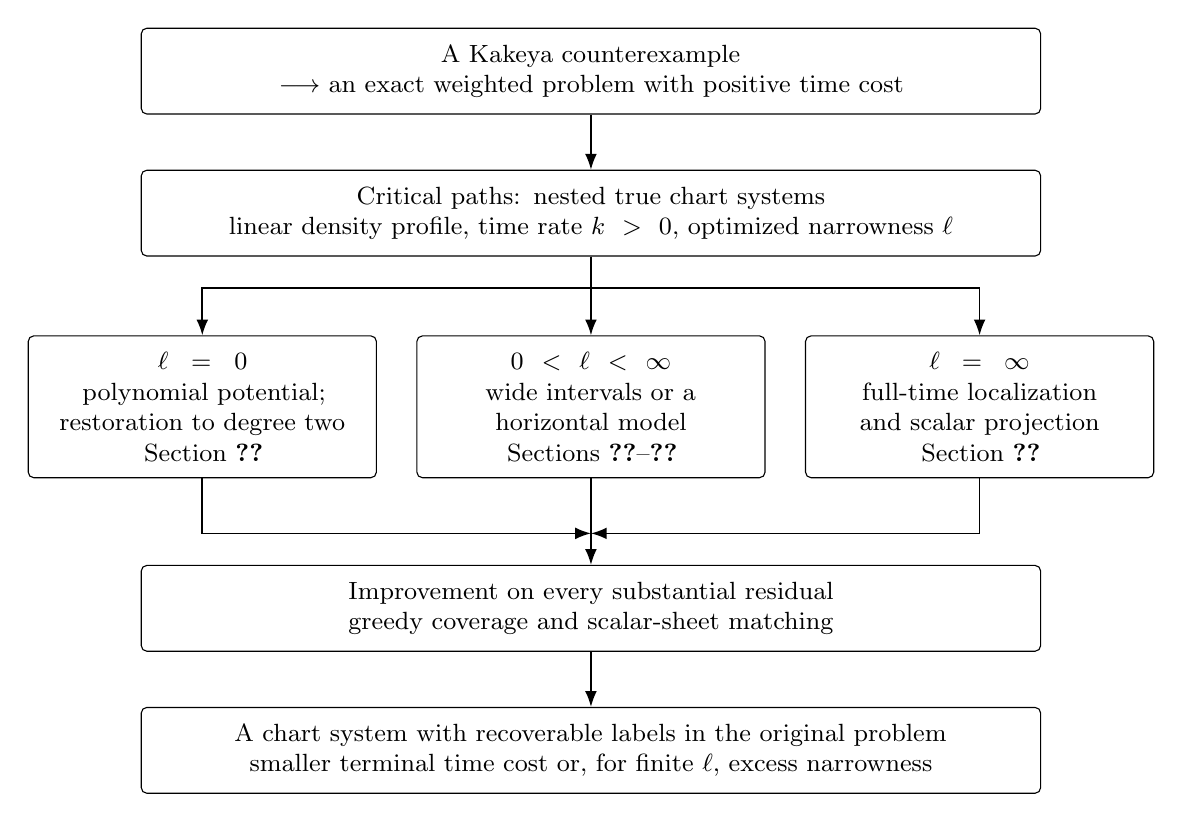
\begin{tikzpicture}[
  box/.style={draw,rounded corners=2pt,align=center,inner sep=6pt,
              font=\small,text width=11cm},
  branch/.style={box,text width=4cm,minimum height=15mm},
  flow/.style={-{Latex[length=2mm]},semithick},
  node distance=7mm and 5mm
]
\node[box] (model) {A Kakeya counterexample\\
  \(\longrightarrow\) an exact weighted problem with positive time cost};
\node[box,below=of model] (path) {Critical paths: nested true chart systems\\
  linear density profile, time rate \(k>0\), optimized narrowness \(\ell\)};
\node[branch,below=10mm of path] (finite) {\(0<\ell<\infty\)\\
  wide intervals or a horizontal model\\
  Sections~\ref{sec:finite-narrowness}--\ref{sec:critical-rates}};
\node[branch,left=of finite] (iso) {\(\ell=0\)\\
  polynomial potential;\\
  restoration to degree two\\
  Section~\ref{sec:isotropic}};
\node[branch,right=of finite] (unbounded) {\(\ell=\infty\)\\
  full-time localization and scalar projection\\
  Section~\ref{sec:unbounded-narrowness}};
\node[box,below=11mm of finite] (candidate) {Improvement on every substantial residual\\
  greedy coverage and scalar-sheet matching};
\node[box,below=of candidate] (atlas) {A chart system with recoverable labels in the original problem\\
  smaller terminal time cost or, for finite \(\ell\), excess narrowness};
\draw[flow] (model)--(path);
\draw[flow] (path.south)--(finite.north);
\draw[flow] (path.south) -- ++(0,-4mm) -| (iso.north);
\draw[flow] (path.south) -- ++(0,-4mm) -| (unbounded.north);
\draw[flow] (finite.south)--(candidate.north);
\draw[flow] (iso.south) |- ([yshift=4mm]candidate.north);
\draw[flow] (unbounded.south) |- ([yshift=4mm]candidate.north);
\draw[flow] (candidate)--(atlas);
\end{tikzpicture}

 \caption{The contradiction from a hypothetical Kakeya counterexample.
 A critical weighted path has one of three narrowness regimes.
 Each produces improvements on substantial residuals, which are
 assembled into a chart system with recoverable labels in the
 original problem. In the middle branch, \(2k=1\) uses the three-leg
 switch; \(2k\ne1\) returns to wide intervals, with a bootstrap
 when \(2k<1\). The scalar version of the isotropic argument supplies
 the projection theorem used in the other two branches.}
 \label{fig:proof-map}
\end{figure}

\subsection{Organization and scale conventions}

Section~\ref{sec:framework} gives the weighted models, chart
normalization, and reduction from an arbitrary Kakeya set.
Section~\ref{sec:comparison} proves the scalar-sheet comparison and
terminal extension. Section~\ref{sec:critical-paths} constructs the
critical paths and proves the criterion that turns local candidates
into forbidden improvements.

Section~\ref{sec:scalar-tools} develops the conditional scalar
estimates, and Section~\ref{sec:isotropic} treats the isotropic
case and its auxiliary scalar model.
Section~\ref{sec:retained-edge-tools} proves the planar rigidity
tools and fits their conclusions to the original incidence edges.
Sections~\ref{sec:finite-narrowness} and~\ref{sec:critical-rates}
use these results to treat finite positive narrowness and its
critical time regimes.
Section~\ref{sec:unbounded-narrowness} treats unbounded narrowness
and completes the proof of Theorem~\ref{thm:main}.
Section~\ref{sec:consequences} develops the dimensional and geometric
consequences.

Two scale conventions are essential when these steps are combined.
Section~\ref{sec:critical-paths} distinguishes the original resolution
\(N_0\) from the local tangent resolution \(N\): returned chart
systems must satisfy mass and list bounds subpower in \(N_0\), even
when the local analysis only supplies bounds subpower in \(N\).
Section~\ref{sec:framework} distinguishes current incidence laws
from earlier witness laws. A witness floor used for counting is
paired with a density cap for that same law.

\section{Weighted models and the reduction from arbitrary Kakeya sets}
\label{sec:framework}

We encode a line family by a probability law on trajectories and a
selection of trajectory--time incidences. A local fit confines the
base spatial projection of each whole trajectory piece to a moving
box and keeps a quadratic polynomial small along that piece. Its mass is measured on the
selected incidences.
Theorem~\ref{thm:model-reduction} turns a hypothetical Kakeya
counterexample into a weighted problem in which fitting at the final
thickness requires a positive power cost in time localization.
The infimum of these costs is the horizon.

We first develop the observations and density estimates used to measure
these fits. We then define the charts, show how their priors and densities
transform under normalization, and prove the reduction from an arbitrary
Kakeya set. All subpower factors in this section refer to one exact
sequence with resolution tending to infinity; later sequences of exact
problems will be introduced separately.

\subsection{Exact problems and observations}

The model has two versions. Version \(2\) retains the lines in
\(\R^4\); version \(1\) is the scalar model used after projection.
In each version a prior samples a trajectory independently of time,
and a separate event specifies which trajectory--time incidences
are retained.

\begin{definition}[Exact problems]\label{def:exact-problem}
An exact problem is a sequence indexed by a real parameter
\(N_0\to\infty\), with a fixed length \(0<L<\infty\).
For \(0\le r\le L\), write \(a_r=N_0^{-r}\).
A subpower factor \(K_0\ge1\) satisfies
\(\log K_0/\log N_0\to0\); its value may be increased from one occurrence
to the next.  We write \(A\sim_{\log}B\) when
\(K_0^{-1}B\le A\le K_0B\) for such a factor.
Subsequences are permitted.

There are finitely many auxiliary worlds \(\gamma\), of weights
\(\omega_\gamma\ge0\) satisfying \(\sum_\gamma\omega_\gamma=1\).
In world \(\gamma\), a trajectory has prior probability law
\(\nu_\gamma\), independently of uniform time \(t\in[0,1]\).
Its base coordinate is
\[
 y(t)=y_0+tV\in\R^j,\qquad |y(t)|+|V|\le K_0.
\]
We use the following two versions.
\begin{enumerate}
\item In version \(1\), \(j=1\), and
\(w(t)=w_0+w_1t+w_2t^2\), with
\(\sup_{[0,1]}|w|\le K_0\).
Tests are \(P(t,y,w)=w-F(t,y)\), where \(F\) is a polynomial of
total degree at most two.  The derivative scale is \(B=1\), and \(X=w\).
\item In version \(2\), \(j=2\), and \(w(t)=w_0+tW\) is affine.
The coefficients of \(w\) need not be independent of those of \(y\).
Each world has a derivative scale \(B>0\) and a polynomial
\(P_*(t,y,w)\) of total degree at most two.  Writing
\(X(t)=P_*(t,y(t),w(t))\), the native bounds are
\begin{align}
 \sup_{[0,1]}|X|&\le K_0,&
 \sup_{[0,1]}|\partial_wP_*|&\le K_0B,
 \label{a01:native-bounds}\\
 |\partial_wP_*|&\ge B/K_0
       \quad\hbox{at selected incidences},&
 |\partial_{ww}P_*|&\le K_0B^2.
 \notag
\end{align}
Tests in this version are arbitrary polynomials \(P(t,y,w)\) of
total degree at most two.
\end{enumerate}
In both versions \(X\) is a quadratic polynomial along each trajectory;
its coefficients are subpower bounded by interpolation on \([0,1]\).

An incidence selection is an event \(E_\gamma\) in trajectory--time
space, and
\begin{equation}
 d\mu_\gamma(l,t)=\1_{E_\gamma}(l,t)\,d\nu_\gamma(l)\,dt,
 \qquad
 \mu=\sum_\gamma\omega_\gamma\mu_\gamma,\qquad
 \mu(\mathrm{all})\ge K_0^{-1}.
 \label{a01:incidence-law}
\end{equation}
Thus \(\mu_\gamma\) is not normalized to probability.
A further selection restricts this event and must retain total mass
at least an inverse subpower.
\end{definition}

Here and below polynomial bounds are \(N_0^M\) for a finite exponent
\(M\) fixed throughout the exact sequence.  The exponent may be
arbitrarily large and may change when a new exact problem is constructed.
We impose the following finiteness convention.

\begin{definition}[Tempered data]\label{a01:tempered}
The numbers of worlds, specified parameter ranges and coefficients,
and \(B,B^{-1}\), are polynomially bounded.  In the full trajectory
coefficient coordinates, each prior has piecewise constant Lebesgue
density, polynomially bounded on polynomially many semialgebraic
pieces.  Trajectory and incidence predicates use polynomially many
polynomial conditions of bounded individual degree, with arbitrary
Boolean combinations.  The number of variables in each geometric
test is bounded.  Real constants in these conditions have no height
restriction.

Exact-level selections, labels, cells, and frames obey such uniform
bounds.  Chart widths and time lengths have polynomially bounded
reciprocals.  Changes of trajectory coordinates are invertible and
have polynomially controlled constant Jacobian.  We permit
polynomially many copies of coefficient space, with an internal
discrete trajectory index.  This index is not a world or an observed
point feature; all assignments concern indexed trajectories.

Measurable arguments may be used to locate a finite family of boxes
or polynomial tests.  The output is encoded by those constants and
geometric tests, not by a description of the intermediate measurable
search.
\end{definition}

Worlds with extremely small success fractions can be removed.
After forming chart worlds, charts with extremely small conditional
prior mass can also be removed: there are only polynomially many
charts, and the selected measure is bounded by prior times time.
The threshold can be a sufficiently small reciprocal polynomial.
These observations preserve the convention in
\Cref{a01:tempered}.

Use nested half-open dyadic grids, rounding requested widths upwards
within a factor of two.  The observation at depth \(r\) is
\begin{equation}
 p_r=(\gamma,t,y(t),[w(t)]_{a_r/B}).
 \label{a01:observation}
\end{equation}
Within a world its density is with respect to \(dt\,dy\) and counting
measure on the hidden bin.  Such densities exist: at fixed \(t\),
replacing \(y_0\) by \(y(t)=y_0+tV\) has Jacobian one.

A density is \emph{typically} \(n=N_0^{-f}\) if, for every fixed
\(\tau>0\), the selected incidences where it is outside
\([N_0^{-\tau}n,N_0^\tau n]\) have total weighted mass at most
\(N_0^{-c(\tau)}\), eventually, for some \(c(\tau)>0\).
One-sided typical bounds have the corresponding meaning.
A problem is homogeneous for a family of observations if each
observation has a common exponent, independent of the world and
fixed along the exact sequence.  Unless otherwise stated the
observations are \(p_r\), \(0\le r\le L\), and their typical densities
are denoted \(n(r)=N_0^{-f(r)}\).

\subsection{Density selection and homogeneous profiles}

The selected observation densities need not initially have uniform
sizes. We will restrict to incidences on which their logarithmic sizes
stabilize. Restrictions and finite refinements obey a simple mass
estimate; a finite-table approximation will make the subsequent density
selections compatible with the tempered data.

\begin{lemma}[Restriction, refinement, and caps]
\label{a01:density-operations}
Let \(g\) be the unnormalized density of an observation and \(g'\)
the density after restriction.  For \(0<\epsilon<1\),
\begin{equation}
 \int_{\{g'<\epsilon g\}}g'\le
 \epsilon\int g.
 \label{a01:restriction-integral}
\end{equation}
If an observation is refined by a discrete label with at most \(D\)
possible values on the retained events, the total refined mass at
entries whose density is less than \(\epsilon g\) is at most
\(\epsilon D\int g\).
These statements apply within conditional worlds and may be
summed with the original world weights.

Consequently further inverse-subpower restrictions, and refinements
by subpower lists, preserve typical logarithmic densities.
Upper density bounds may be integrated over arbitrary base regions
and summed over discrete entries after the exceptional observations
have been removed.
\end{lemma}

\begin{proof}
Restriction gives \(0\le g'\le g\), and integrating the defining
inequality on \(\{g'<\epsilon g\}\) proves
\Cref{a01:restriction-integral}.  For a refinement with densities
\(g'_c\), sum the inequalities \(g'_c<\epsilon g\) over at most \(D\)
labels at each old observation and then integrate.
Take \(\epsilon=N_0^{-\tau}\), and absorb a subpower \(D\) or a
subpower normalization loss into a smaller positive power.

For clarity about exceptional sets, write the pushed-forward
measure as a good part plus an omitted part, with densities
\(g_{\mathrm{good}},g_{\mathrm{bad}}\).
On the new states where \(g_{\mathrm{bad}}>g_{\mathrm{good}}\),
their total mass is at most \(2\int g_{\mathrm{bad}}\).
On the other states the total density is at most twice the good
density.  This transfers a ceiling proved for the restricted good
measure to a typical ceiling for the full resulting measure.
It does not justify summing an unremoved exceptional portion
against small conditional probabilities.
\end{proof}

A datum is \emph{known by \(p_s\)} if, after permitted pruning, it
belongs to a deterministic list of size at most \(K_0\) depending
only on \(p_s\).  List knowledge, rather than a choice of one
representative, is the convention throughout.
The exact base coordinates in an observation vary continuously.
To choose labels or density ranges while preserving temperedness, we
approximate their joint law on a sufficiently fine finite base mesh.
The next lemma controls the error uniformly over subsequent choices.

\begin{lemma}[Joint base flattening]\label{a01:flattening}
Fix tempered discrete labels and predicates of polynomial total
count.  Given a fixed \(T>0\), there is a fixed finite \(D\) such that
uniformly redistributing the base \((t,y)\) inside its mesh cells
of width \(\rho\sim N_0^{-D}\), while retaining the discrete entries,
changes the joint measure in total variation by \(O(N_0^{-T})\).
Thus a posterior list selector for these entries can be replaced,
with that error in success, by a cell-constant tempered list table.
\end{lemma}

\begin{proof}
Use coordinates \((t,y,V)\) and the remaining trajectory
coefficients, extending all densities by zero outside their
domains.  Holding the other variables fixed, each polynomial
condition has a bounded number of changes on a base-coordinate
axis, unless it is identically zero there; the latter condition
has no changes.  There are polynomially many conditions.
The weighted density and the discrete labels therefore change
across only polynomially many boundaries on each such fiber.
Their heights and the ranges of the remaining variables are
polynomially bounded.  Integration first on the fiber and then in
the other variables shows that a base translation of size at most
\(\rho\) changes the joint measure by at most
\(N_0^C\rho\), with \(C\) fixed by the tempered bounds.
Sum over the finitely many base axes and over internal index copies.

Within-cell averaging has the same bound, up to a dimensional
constant: write its \(L^1\) difference from the original density
as the integral of pairwise differences of density values in the
same cell, then compare these with translations of length at most
a constant times \(\rho\).  Choosing \(D>C+T+1\) proves the assertion.
All labels are included in this argument jointly.

A measurable selector has the same success up to total variation
error on the flattened law.  On that law the posterior of the
discrete entries is constant inside each cell with its conditioning
bins fixed; a constant maximizing list can be chosen there.
There are polynomially many such cells and entries.  The resulting
lookup table is tempered, and its success transfers back by the
same total variation estimate.
\end{proof}

When two grids overlap with at most \(K_0\) members at fixed exact
base and other conditioning data, their common refinement has the
same typical exponent by \Cref{a01:density-operations}.
For a one-way upper bound it suffices to sum the good measure over
the corresponding covering entries.

\begin{lemma}[Homogenization]\label{a01:homogenization}
After a tempered further selection of inverse-subpower mass and a
subsequence, an exact problem has a homogeneous profile \(f(r)\)
on every prescribed compact depth interval.  It is nondecreasing
and \(1\)-Lipschitz.  Jointly, one may homogenize the observation
\((p_r,[V]_{a_u})\) on compact nonnegative \((r,u)\)-ranges, obtaining
a function \(f(r,u)\) that is nondecreasing in each variable and
has Lipschitz constants \(1\) in \(r\) and \(j\) in \(u\).
Moreover \(f(r,0)=f(r)\).
\end{lemma}

\begin{proof}
Choose a countable dense depth grid containing all required
endpoints.  At stage \(N_0\), test a finite initial part of this
grid, increasing its size sufficiently slowly.
By \Cref{a01:flattening}, use a common fixed polynomial base mesh
fine enough for all the observations and for a power-small
total variation error.  The tested hidden and velocity grids
are nested and lie in fixed compact depth ranges, so their joint
entries are determined by the finest tested bins.  Their total
number, including base cells, is polynomial.

Polynomial bounds give a polynomial ceiling for each flattened
density.  Densities below \(N_0^{-C}\), for a sufficiently large
fixed \(C\), have power-small total mass, by summing over the
polynomial ranges and entries.  Quantize the remaining logarithmic
densities in intervals of width \(\epsilon_{N_0}\to0\).
If \(m_{N_0}\) is the number of tested observations, choose the
rates so slowly that the number of density-type lists is
\[
 \bigl(O(\epsilon_{N_0}^{-1})\bigr)^{m_{N_0}}=N_0^{o(1)}.
\]
One list carries inverse-subpower mass.  Restrict to it.
This restriction is a cell table testing the joint discrete
observations and is tempered.  Its upper bounds persist, and
\Cref{a01:density-operations} shows that its densities lose a
fixed power relative to the preselection values only on
power-small mass.

The total variation estimate transfers these conclusions to
the exact base densities.  Indeed, where two densities differ
by a large multiplicative factor, their \(L^1\) difference
controls the mass under the larger density there.
Pass to a subsequence on which the type exponents converge at
every fixed tested depth.

Refinement from depth \(r\) to \(r'\ge r\) has at most
\(K_0N_0^{r'-r}\) hidden-bin choices, and refinement from velocity
depth \(u\) to \(u'\ge u\) has at most
\(K_0N_0^{j(u'-u)}\) choices.  Monotonicity of densities under
refinement and \Cref{a01:density-operations} imply
\begin{align*}
 0&\le f(r',u)-f(r,u)\le r'-r,\\
 0&\le f(r,u')-f(r,u)\le j(u'-u).
\end{align*}
These inequalities extend the profiles uniquely to all
intermediate depths; nesting squeezes their typical densities
between nearby tested ones.  Since \(|V|\le K_0\), appending
the unit velocity bin costs only \(K_0\) choices, proving
\(f(r,0)=f(r)\).
\end{proof}

Other fixed logarithmic quantities with polynomial upper and
reciprocal bounds may be homogenized by the same argument.
In subsequent cap estimates, fixed tolerances on fixed finite
grids are sent to zero sufficiently slowly, and the grids
increase sufficiently slowly, that the exceptional mass is
negligible compared with the particular inverse-subpower
selection in use.  This convention concerns the present exact
\(N_0\)-sequence.

The class used in the contradiction imposes two further bounds.
The first limits how rapidly the typical density can decrease
as the hidden observation is refined toward the terminal depth.
The second limits velocity concentration within a terminal
observation.

\begin{definition}[The cap class]\label{a01:cap-class}
Fix \(S,\eta>0\).  A homogeneous exact problem belongs to \(C(d)\),
\(d<1\), if
\begin{equation}
 f(L)-f(r)\le d(L-r)\qquad(0\le r\le L),
 \label{a01:endpoint-cap}
\end{equation}
and, for \(0<u\le\eta L\), the joint density of
\((p_L,[V]_{a_u})\) has typical upper bound
\begin{equation}
 n(L)N_0^{-Su+o(1)}.
 \label{a01:angular-cap}
\end{equation}
The \(o(1)\) is interpreted by the fixed-tolerance convention above.
The parameters \(S,\eta\) are held fixed when the class is used.
\end{definition}

\begin{lemma}[Angular caps under coarsening]\label{a01:angular-coarsening}
Suppose \Cref{a01:angular-cap} holds. For \(0\le b<L\) and
\(0<u\le\eta L\), the conditional probability
\[
 \Pp\{[V]_{a_u}=v\mid p_b\},
 \qquad v=[V]_{a_u},
\]
under the selected incidence law has typical upper bound
\(N_0^{-Su+o(1)}\), evaluated at the sampled angular entry.
Normalizing the total incidence mass does not change this
conditional distribution. Good restricted measures with subpower
slack can be prepared simultaneously on slowly increasing finite
depth grids, losing negligibly relative to a specified
inverse-subpower selection.
\end{lemma}

\begin{proof}
Fix the exponents and a tolerance.  Remove the fine entries where
the joint angular upper bound or the pure \(p_L\) lower bound fails.
For each remaining fine entry and a specified angular bin, its
restricted numerator is bounded by
\(N_0^{-Su+O(\tau)}\) times the old pure density.
Sum these numerators over the fine hidden bins inside a coarse bin
before dividing by the corresponding sum of old pure densities.
This proves the coarse bound for the good submeasure relative to
the old denominator.  The omitted-mass comparison in
\Cref{a01:density-operations} gives the typical assertion, and
\Cref{a01:restriction-integral} handles a later inverse-subpower
restriction of the denominator.

For finitely many tests their power-small exceptions can be
summed.  Choose the tolerance and number of tests slowly to
obtain the final assertion.  These exclusions may be purely
analytical; if an output selection needs them,
\Cref{a01:flattening} implements the corresponding cell tests.
In particular this argument does not assert a bound on the
maximum angular probability over all bins of an unpruned law.
\end{proof}

\subsection{Time charts and prior-mass budgets}

We now describe the local fits whose time cost defines the horizon.
A chart controls each assigned trajectory throughout its time
interval. Its incidence selection specifies where the lower
derivative bound is required and supplies the mass entering the
true floor. This selection need not occupy the whole interval.

\begin{definition}[Charts, true packets, and known atlases]
\label{def:true-chart}
At depth \(r\in(0,L]\), a chart system has a common dyadic
time partition into intervals \(I\) of length
\(q=N_0^{-h+o(1)}\), \(h\ge0\).
Within each world and each interval, it assigns disjoint
trajectory sets \(A_c\) to chart labels \(c\), and selects
incidences from the given event on these assignments.
The total selected mass is at least \(K_0^{-1}\).

A chart has an affine spatial center \(y_c(t)\) and an
invertible matrix \(D_c\), with
\begin{equation}
 \|D_c\|\le qK_0,\qquad J_c=|\det D_c|,\qquad
 \sup_{t\in I}|D_c^{-1}(y(t)-y_c(t))|\le K_0
       \quad(l\in A_c).
 \label{a01:chart-space}
\end{equation}
It has a test of the appropriate model class satisfying
\begin{align}
 \sup_{t\in I}|P(t,y(t),w(t))|&\le K_0a_r,
 &
 \sup_{t\in I}|\partial_wP(t,y(t),w(t))|&\le K_0B,
 \label{a01:chart-test}\\
 |\partial_wP|&\ge B/K_0
       \quad\hbox{on its selected incidences},
 &
 |\partial_{ww}P|&\le K_0B^2/a_r.
 \notag
\end{align}
All chart data, assignments, selections, inverse coordinate
changes, and reciprocal widths are tempered.

Write
\[
 \nu_c=\nu_{\gamma(c)}(A_c),\qquad
 m_c=\mu_{\gamma(c)}(\hbox{selected incidences assigned to }c).
\]
A \emph{packet} is an individual chart together with its label,
time interval, geometric and test data, full trajectory assignment
\(A_c\), and current incidence selection. It carries the assigned
trajectory measure \(\nu_{\gamma(c)}|_{A_c}\), of mass \(\nu_c\),
and the unnormalized selected incidence measure, of mass \(m_c\).
An incidence-only restriction shrinks the latter without
conditioning the assigned trajectory measure on success.
A packet is \emph{true} when
\begin{equation}
 \frac{m_c}{q}\ge K_0^{-1}n(r)J_c.
 \label{a01:true-floor}
\end{equation}
A system is \emph{true} if every used packet is true.
A \emph{known atlas} at depth \(r\) is a chart system whose
label is known by \(p_L\). It has all the assignment, coverage,
geometric, test, and temperedness properties above, but need not
satisfy \Cref{a01:true-floor}.
We also allow known atlases at \(r=0\), with \(a_0=1\),
when the same displayed bounds hold.
\end{definition}

Since \(y-y_c\) is affine on \(I\), \Cref{a01:chart-space}
also bounds \(qD_c^{-1}(V-y_c')\) by \(K_0\).
Disjointness of assignments in each interval gives the basic
budget
\begin{equation}
 m_c\le q\nu_c,\qquad
 \sum_c\omega_{\gamma(c)}q\nu_c\le1.
 \label{a01:assignment-budget}
\end{equation}
The sum includes all worlds, intervals, and labels of one system.

The following elementary estimate converts the small-value and
lower-derivative tests into a bound on the hidden-coordinate bins.

\begin{lemma}[Quadratic sublevel sets]\label{lem:quadratic-sublevel}
Let \(Q\) be a real polynomial of degree at most two, and let
\(\varepsilon,b,\delta>0\). The set
\[
 \{w\in\R:|Q(w)|\le\varepsilon,
                  \ |Q'(w)|\ge b\}
\]
has total length at most \(4\varepsilon/b\) and meets at most
\(C(1+\varepsilon/(b\delta))\) bins of any grid of width
\(\delta\), for an absolute constant \(C\).
\end{lemma}

\begin{proof}
The condition \(|Q'|\ge b\) is the union of at most two
intervals on each of which \(Q\) is monotone. On either
interval, the inverse derivative bound gives length at most
\(2\varepsilon/b\) for the indicated sublevel set.
Each resulting interval meets at most two more grid bins than
its length divided by \(\delta\).
\end{proof}

The defining true floor compares incidence mass with observation
density and spatial volume. The next lemma combines that floor
with the assignment budget to obtain comparability with the prior
mass \(\nu_c\), and also confines the chart label to a subpower
list determined by the observation.

\begin{lemma}[Saturation and label knowledge]\label{a01:saturation}
A true system may be restricted, retaining inverse-subpower
total mass and enlarging subpower slacks, so that every used
chart satisfies
\begin{equation}
 \frac{m_c}{q}\sim_{\log}\nu_c\sim_{\log}n(r)J_c,
 \label{a01:saturated-floor}
\end{equation}
and its label is known by \(p_r\).
The true floor persists on the resulting selected incidences.
\end{lemma}

\begin{proof}
For a large subpower \(H\), deleting charts with
\(q\nu_c>Hm_c\) loses at most
\[
 \sum_{q\nu_c>Hm_c}\omega_{\gamma(c)}m_c
 \le H^{-1}\sum_c\omega_{\gamma(c)}q\nu_c\le H^{-1}.
\]
Choose \(H^{-1}\) negligible relative to the system mass.

Analytically remove the exceptional \(p_r\)-entries above the
ceiling \(K_0n(r)\), choosing the slack so the removed mass is
negligible relative to that same mass.
At a fixed base in chart \(c\), the conditions
\(|P|\le K_0a_r\) and \(|P_w|\ge B/K_0\) admit only \(K_0\)
hidden bins of width \(a_r/B\).
Apply \Cref{lem:quadratic-sublevel} with
\(\varepsilon=K_0a_r\), \(b=B/K_0\), and
\(\delta=a_r/B\), and enlarge the subpower factor.
The chart base volume is at most \(K_0qJ_c\).
Thus the good portion of \(m_c\) is at most \(K_0n(r)qJ_c\).
Discard whole charts whose full mass is more than twice this
bound.  Their total mass is controlled by twice the globally
omitted mass.  Together with the first deletion and the true
floor, this proves \Cref{a01:saturated-floor} before a final
enlargement of the slack.

To obtain lists, let a chart cross an observation if its time,
spatial, value, and event-derivative tests are compatible with
that observation.  If \(T(p_r)\) is the number of crossings,
the same volume calculation, now integrating the capped
original measure rather than only assigned incidences, gives
\begin{align*}
 \int T(p_r)\,d\mu_{\mathrm{cap}}
 &\le K_0\sum_c\omega_{\gamma(c)}n(r)qJ_c\\
 &\le K_0\sum_c\omega_{\gamma(c)}m_c.
\end{align*}
Markov's inequality, with a sufficiently large subpower
threshold, leaves subpower lists and loses negligible system
mass.  The joint flattening lemma implements these lists
as tempered tables if necessary.
Finally discard charts that lost more than half their
selected mass in these operations.  Their total loss is
at most twice the removed incidence mass, and
\Cref{a01:true-floor} survives with enlarged slack.
\end{proof}

Later restrictions can reduce the selected mass of an individual
chart. The next lemma gives two ways to continue a count: restore
a floor for the current entries by pruning, or charge earlier
witnesses using a cap for their own frozen measure.

\begin{lemma}[Restoring current floors and charging witnesses]
\label{a01:witness-budgets}
Fix a chart layer with the assignment budget
\Cref{a01:assignment-budget}.  Suppose a later selected measure
has inverse-subpower mass in the same normalization.
For each chart let at most \(D\le K_0\) additional entries be
used, and let \(\widetilde m_{c,e}\) be their current masses.
For any \(0<\epsilon<1\), deleting entries with
\begin{equation}
 \widetilde m_{c,e}<\frac{\epsilon q\nu_c}{D}
 \label{a01:current-floor}
\end{equation}
loses at most \(\epsilon\) total weighted mass.
In particular, \(\epsilon\) may be an inverse-subpower
negligible relative to the current total mass, giving
current floors against the full assignment budget.
For finitely many prescribed layers, allocate positive tolerances
\(\epsilon_i\) with \(\sum_i\epsilon_i\le\epsilon\). Their
corresponding floors can be achieved on one final retained measure,
with total weighted loss at most \(\epsilon\).

If time is further partitioned, the corresponding threshold
uses \(|I'|\nu_c\) for a subinterval \(I'\subset I\);
summing these budgets over the subintervals gives \(q\nu_c\).

For a collection of disjoint witness submeasures of a fixed
measure \(\lambda\), all supported in a domain \(U\), the total
witness mass is at most \(\lambda(U)\). With multiplicity at
most \(D\), the bound is \(D\lambda(U)\). Any cap used in this
count must hold for that same fixed measure \(\lambda\).
No floor on an arbitrary later restriction is thereby asserted.
\end{lemma}

\begin{proof}
Sum \Cref{a01:current-floor} over at most \(D\) entries per
chart, and then use \Cref{a01:assignment-budget}.
For finitely many layers, choose positive tolerances
\(\epsilon_i\) with \(\sum_i\epsilon_i\le\epsilon\), and use
\(\epsilon_i\) in the threshold for layer \(i\). Keep its assignment
budgets and entry counts fixed. Repeatedly delete all remaining
incidences of any entry whose current mass is positive and below its
fixed threshold,
reconsidering every layer after each deletion. An entry becomes empty
permanently when deleted, so it is charged at most once. The assignment
budget bounds the weighted charges from layer \(i\) by
\(\epsilon_i\), including deletions caused by earlier losses in other
layers. There are finitely many entries, so the process terminates
with every surviving entry meeting its threshold in the final measure
and total loss at most \(\epsilon\). The removed entries form a
polynomially sized table of original predicates, preserving temperedness.
For a slowly increasing collection satisfying the standing tempered
bounds, choose its size and tolerance allocation slowly enough that
the floor losses remain subpower.
The time-subinterval assertion follows from
\(\sum_{I'\subset I}|I'|\nu_c=q\nu_c\).

For the last assertion, if the witnesses of the counted
labels are disjoint submeasures of a frozen measure
\(\lambda\) and all lie in a domain \(U\), the sum of their
masses is at most \(\lambda(U)\).  A multiplicity bound \(D\)
replaces this by \(D\lambda(U)\).
The cap and the witnesses must therefore refer to the same
measure \(\lambda\), after every restriction required for that
cap has been imposed. A floor for these frozen witnesses gives no
lower bound for a later restriction; the first part of the lemma
provides a floor for that current measure.
\end{proof}

\begin{lemma}[Fullness of the largest spatial scale]
\label{a01:largest-axis}
In a cap-class problem, a chart system known by \(p_L\),
whether true or not, has
\[
 \|D_c\|\sim_{\log}q
\]
on an inverse-subpower selection, after homogenizing the
ratio if necessary.
\end{lemma}

\begin{proof}
The upper bound is part of \Cref{a01:chart-space}.
If the ratio were at most \(N_0^{-\alpha}\) for a fixed
\(\alpha>0\) on inverse-subpower mass, the endpoint bounds
in \Cref{a01:chart-space} would confine \(V\), for each
chart, to a ball of radius \(K_0N_0^{-\alpha}\) about \(y_c'\).
Choose a fixed \(u>0\) with \(u<\alpha/2\) and \(u\le\eta L\).
Such a ball meets only \(K_0\) velocity bins of width \(a_u\).
Since chart labels are known by \(p_L\), at each retained
terminal observation only \(K_0\) such velocity bins are
needed.  On the good restricted measure each has numerator
at most \(N_0^{-Su+o(1)}\) times the old pure denominator,
by \Cref{a01:angular-cap}.  Summing these bounds and then
integrating shows that the alleged mass is power-small.
The exceptional entries were removed before this sum.
This contradiction excludes every fixed-power deficiency.
\end{proof}

\subsection{Normalization, composition, and horizon}

To iterate the construction, we regard each chart as a new world
with its conditional trajectory prior and its own unit time
interval. The density transformation must be tracked within that
world before child charts can be lifted back to the original
problem. The following lemma records both operations and the
label-knowledge condition needed for intermediate true floors.

\begin{lemma}[Chart normalization and lifting]\label{lem:normalization}
Let a homogeneous exact problem of length \(L\) have a
terminal-known atlas at depth \(0\le r<L\).
After discarding extremely light charts and homogenizing
their Jacobians and prior masses, it defines a new
homogeneous exact problem of length \(L'=L-r\).
For its typical densities,
\begin{align}
 n'(L')&\sim_{\log}
       n(L)\frac{J_c}{\nu_c},
 \label{a01:terminal-normalization}\\
 n'(s)&\le N_0^{o(1)}
       n(r+s)\frac{J_c}{\nu_c}
       \qquad(0\le s<L').
 \label{a01:intermediate-normalization}
\end{align}
If the parent label is already known by \(p_r\), there is
equality up to subpower factors in
\Cref{a01:intermediate-normalization}.
The class \(C(d)\), with the same \(S,\eta\), is preserved.

A true terminal system in the new problem lifts to a true
terminal system in the old problem.  Intermediate true
systems also lift through a parent with the stated
intermediate density equality, in particular through a
prepared true parent.
\end{lemma}

\begin{proof}
Put
\[
 Z=\sum_c\omega_{\gamma(c)}q\nu_c,\qquad
 \omega'_c=\frac{\omega_{\gamma(c)}q\nu_c}{Z}.
\]
If the atlas success is \(M\ge K_0^{-1}\), then
\(M\le Z\le1\).  Use \(c=(\gamma,I,A_c)\) as a new world,
with trajectory law \(\nu_\gamma(\,\cdot\,|A_c)\) and
independent uniform time
\[
 t=t_c+q\tau,\qquad
 y=y_c(t)+D_cz,\qquad 0\le\tau\le1.
\]
The new selected measure is the pushforward of the old
assigned selected measure divided by \(q\nu_c\).
Its weighted total is the old atlas selected mass divided
by \(Z\).  In particular it is still a restriction of the
new product priors and has inverse-subpower mass.

In version \(1\), if the parent test is \(w-F(t,y)\), set
\[
 w'=\frac{w-F(t,y)}{a_r}.
\]
This is quadratic along trajectories and bounded by \(K_0\).
In version \(2\), retain \(w\) and use the native test
\(P_*'=P/a_r\), with derivative scale \(B'=B/a_r\).
The parent test bounds give
\[
 \sup|P_*'|\le K_0,\quad
 \sup|\partial_wP_*'|\le K_0B',\quad
 |\partial_wP_*'|\ge B'/K_0,\quad
 |\partial_{ww}P_*'|\le K_0(B')^2
\]
in the required places.  All base and velocity bounds
follow from \Cref{a01:chart-space}.
At \(r=0\), if the existing native test already has these
bounds after the spatial normalization, it may instead be
retained unchanged; this is useful for full-time
spatial atlases.

These coordinate changes preserve the permitted models.
Their maps on coefficient space have constant Jacobian:
the base changes are affine, and in version \(1\) the
subtraction of the quadratic \(F(t,y)\) is triangular
with respect to the \(w\)-coefficients.
They and their inverses have polynomial control.
Charts whose conditional prior is below a sufficiently
small reciprocal polynomial have negligible total
success, by polynomial chart count.  On the remaining
charts conditioning preserves temperedness.

At fixed old base and chart label, new hidden-bin width
at depth \(s\) is the old width \(a_{r+s}/B\), with a
chart- and base-dependent offset in version \(1\).
The two grids have bounded overlap.
For transported bins, the exact within-world density
transformation is
\begin{equation}
 \rho'_c
 =\frac{qJ_c}{q\nu_c}\rho_c
 =\frac{J_c}{\nu_c}\rho_c.
 \label{a01:exact-density-transform}
\end{equation}
The numerator \(qJ_c\) is the base Jacobian; the denominator
\(q\nu_c\) normalizes the new product prior.
Neither the world weight nor \(Z\) belongs in this
within-world factor.

Refining \(p_L\) by the known chart label does not change
its typical density exponent.  Apply
\Cref{a01:exact-density-transform}, the bounded bin overlap,
and \Cref{a01:density-operations} to obtain
\Cref{a01:terminal-normalization}.  Global exceptional
masses are multiplied by \(Z^{-1}\le K_0\), so their
power-small character is preserved.
At an earlier depth, refinement by an arbitrary label
can only decrease the unnormalized density, giving
\Cref{a01:intermediate-normalization}.  Knowledge by
\(p_r\), and hence by finer hidden observations, gives
the reverse typical inequality.
For a saturated true parent the formulas simplify to
\[
 n'(s)\sim_{\log}\frac{n(r+s)}{n(r)},\qquad
 n'(0)\sim_{\log}1.
\]

For the angular bound, a new velocity bin of width
\(N_0^{-u}\) maps by
\(V=y_c'+D_cV'/q\) into an old velocity ball of radius
\(K_0N_0^{-u}\).  At each exact chart and base it requires
only \(K_0\) old terminal/angular bins.
Sum the good old joint numerators before applying the
density transformation.  The old exceptional mass and
the new states where it dominates are handled as in
\Cref{a01:density-operations}.  This gives
\[
 \rho'_{\mathrm{joint}}\le
 N_0^{o(1)}n(L)\frac{J_c}{\nu_c}N_0^{-Su}
 \sim_{\log} n'(L')N_0^{-Su}
\]
for \(u\le\eta L'\).
Finally,
\[
 \log_{N_0}\frac{n'(s)}{n'(L')}
 \le f(L)-f(r+s)+o(1)
 \le d(L'-s)+o(1),
\]
which proves the endpoint cap.

For lifting, let a child have relative time length
\(q_d\), spatial Jacobian \(J_d\), and selected mass
\(m'_d\) in the new world.  Its old quantities are
\begin{equation}
 q_{cd}=qq_d,\qquad J_{cd}=J_cJ_d,\qquad
 m_{cd}=q\nu_c\,m'_d,\qquad
 \frac{m_{cd}}{q_{cd}}=
       \nu_c\frac{m'_d}{q_d}.
 \label{a01:composition-masses}
\end{equation}
At the terminal depth, a child true floor and
\Cref{a01:terminal-normalization} give the old floor
\(K_0^{-1}n(L)J_cJ_d\).
At an intermediate depth the same conclusion uses the
intermediate equality; an upper bound alone would not
suffice.

The tests lift by multiplication by \(a_r\).
In version \(1\), a child test \(w'-G(\tau,z)\) becomes
\[
 w-F(t,y)-a_rG(\tau,z),
\]
which is still of the special quadratic form.
In version \(2\), \(a_rQ(\tau,z,w)\) remains quadratic,
has old derivative scale \(B\), and satisfies
\[
 |\partial_{ww}(a_rQ)|
 \le K_0a_r\,\frac{(B/a_r)^2}{a_s}
 =K_0\frac{B^2}{a_{r+s}}.
\]
The small-value and first-derivative bounds transform
in the same way.  Spatial matrices and times compose,
whole-block fitting is preserved, and assignments may
record the entire path with nested time partitions.
All operations retain tempered bounds.
\end{proof}

In version \(2\), largest-axis fullness gives a geometric
interpretation to
\begin{equation}
 \log_{N_0}\frac{q^2}{J_c},
 \label{a01:narrowness}
\end{equation}
which we call the narrowness in the specified depth units:
it is the additional thinness of the smaller spatial axis,
up to subpower factors.
Under composition,
\[
 \frac{q_{cd}^2}{J_{cd}}
 =\frac{q^2}{J_c}\frac{q_d^2}{J_d}.
\]
Thus narrowness exponents add exactly, without any
assumption that the spatial axes are parallel.
Statements about a common value of this exponent use a
homogeneous subfamily.

\begin{definition}[Minimum horizon]\label{def:horizon}
For a homogeneous exact problem \(E\) of length \(L\), let
\(H(E)\) be the infimum of the exponents \(h\ge0\) for which
a true system at terminal depth \(L\) exists.
The infimum includes systems on arbitrary subsequences
and further permitted incidence selections, in the
coordinates of \(E\).  Such selections do not change
the terminal density exponent.
\end{definition}

The rest of the section proves two complementary bounds.
Every homogeneous exact problem satisfies \(H(E)\le L\):
terminal fits can be built on intervals of length comparable to
\(a_L\).
A hypothetical Kakeya counterexample, however, yields a cap-class
problem with \(H(E)>0\). Both arguments use the weighted plank
estimate below.

\subsection{The weighted plank input and the initial horizon bound}

We first prove that true terminal systems always exist with horizon
at most \(L\). At time scale \(a_L\), the native quadratic signal
already supplies the polynomial test. A weighted plank estimate
will supply spatial boxes whose incidence mass meets the true floor.

\begin{lemma}[Weighted full-time plank estimate]
\label{lem:weighted-planks}
Fix a bounded affine-line chart in \(\R^2\), and a fixed
permitted enlargement of mesh cells.
For every \(\eps>0\), there are \(\eta_\eps>0\) and
\(C_\eps<\infty\) with the following property.
Let
\[
 M_i(t)=b_i+tu_i,\qquad 0\le t\le1,
\]
be finitely many indexed traces, with \(b_i,u_i\) in the
fixed bounded chart, and arbitrary positive weights
\(\omega_i\).  Repeated traces are allowed.
Let \(D\ge1\), \(\rho=D^{-1}\), and suppose that every
full-time plank
\[
 \mathcal P=\left\{(t,x):
 \begin{array}{l}
 0\le t\le1,\\
 |\langle x-c-tv,e_1\rangle|\le a\rho,\\
 |\langle x-c-tv,e_2\rangle|\le b\rho
 \end{array}\right\},
 \qquad 1\le a\le b\le D,
\]
where \((e_1,e_2)\) is an arbitrary orthonormal spatial
frame and \(c,v\in\R^2\), satisfies
\begin{equation}
 \sum_{i:\,M_i\subset\mathcal P}\omega_i\le Aab.
 \label{a01:weighted-plank-cap}
\end{equation}
Fixed dilations of these plank tests are permitted.
Mark time bins \(J_i\), each of length \(\rho\), with
\(\#J_i\ge D^{1-\eta_\eps}\).
If \(E_{\mathrm{vis}}\) is the union of the spatial--time
mesh cells visited at their bin centers, or fixed
enlargements of those cells, then
\begin{equation}
 \sum_i\omega_i\#J_i
 \le C_\eps A D^\eps\,\#E_{\mathrm{vis}}.
 \label{a01:weighted-plank-conclusion}
\end{equation}
\end{lemma}

\begin{proof}
This is the indexed weighted formulation of
\citet[Lemma~2.3]{ThreeDimensional}.
The plank condition concerns containment of the entire
trace, not merely its marked portions.
The cited statement permits arbitrary positive weights
and repeated indices, and has precisely the long-mark
hypothesis above.
\end{proof}

We record explicitly two extensions of use below.
A continuous weighted law of bounded affine traces can be
rounded in coefficient space at a mesh much smaller than
\(\rho\).  Group traces with the same rounded coefficients
and the same finite mark set, and assign each group its
total prior mass.  This gives a finite indexed family for
\Cref{lem:weighted-planks}.  Fixed enlargements of cells and
planks recover the original traces, and do not alter the
estimates beyond constant factors.  These finite
approximations are used for the estimate; their mark
sets need not be output labels of a chart construction.

Also suppose the chart parameters are bounded by a
subpower \(K_0\), the mesh is a fixed power of \(N_0^{-1}\),
and the available labeled lengths are at least \(K_0^{-1}\).
A common spatial rescaling by a subpower places the traces
in a fixed bounded chart.  Refining meshes and enlarging
cells by subpower factors changes all mark and cell
counts by subpower factors.  The long-mark condition is
then satisfied for every fixed \(\eps>0\) at sufficiently
large \(N_0\).  Choose \(\eps\downarrow0\) only after these
fixed-\(\eps\) requirements, by a slow diagonal.
The factors \(C_\eps D^\eps\) are thereby subpower.
In physical widths \(u,v\), the resulting conclusion
bounds raw weighted average multiplicity by a subpower
times the supremum of
\(\rho^2\sum_{M_i\subset\mathcal P}\omega_i/(uv)\).
This is the form used when a plank is inferred from a
small visited-cell set.

\begin{proposition}[Initial horizon bound]\label{a01:horizon-bound}
Every homogeneous exact problem satisfies \(H(E)\le L\).
\end{proposition}

\begin{proof}
Choose a dyadic \(q\sim a_L\).
In each world and each \(q\)-interval \(I\), group
trajectories by \(y\) at the midpoint of \(I\), to width
\(q\), and by \(X\) there, to width \(a_L\).
Call the joint label \(G\).
Along the block, both \(y\) and \(X\) move by at most
\(K_0q\): for \(X\), use its quadratic coefficients and
the uniform bound in the exact problem.
At an observed incidence, the hidden bin determines \(X\)
to \(K_0a_L\).  In version \(2\), Taylor's formula in \(w\)
uses the native first-derivative and curvature bounds;
the curvature contribution is \(O(K_0a_L^2)\).
Thus \(G\) is known by \(p_L\) up to subpower lists.

Let \(b_G\) be the \(X\)-bin center.
Use the test \(w-b_G\) in version \(1\), or \(P_*-b_G\)
in version \(2\).
It has the required terminal small-value and derivative
bounds throughout the block and at selected incidences.
It remains to find spatial planks carrying the true mass
floor.

Translate by the spatial bin center and divide spatial
coordinates by \(Rq\), where \(R\) is a sufficiently
large subpower.  Normalize block time to \([0,1]\).
All normalized affine traces then lie in one fixed
bounded chart.  Put \(J_0=(Rq)^j\).
In these coordinates use the old trajectory measure
inside \(G\), without normalizing it to a probability;
only time is normalized to the block.
The typical exact-base density in this group is at least
\(n(L)J_0\) up to subpower factors: refine by the known
label \(G\), change coordinates, and sum over compatible
hidden bins.

Choose a common mesh \(\rho=D_m^{-1}\sim N_0^{-D}\),
with \(D_m\) dyadic.  Here \(D\) is fixed sufficiently
large for the tempered bounds and total variation
errors, before the loss parameters below are chosen.
Joint flattening transfers the preceding lower bound
to the cell averages, apart from power-small exceptional
mass, weighted over all worlds, groups, and blocks in
original time.  Coordinate changes and block
normalizations have only polynomial costs.

Fix \(0<\xi<1\).
In each group greedily select spatial planks with
arbitrary time-independent orthonormal spatial frames, affine centers, and
normalized half-widths
\(\rho\le r_i\lesssim1\), \(1\le i\le j\).
A plank may be selected if the remaining incidence mass
on trajectories wholly contained in it, with block time
normalized, is at least
\begin{equation}
 N_0^{-\xi}n(L)J_0\prod_{i=1}^j r_i.
 \label{a01:greedy-threshold}
\end{equation}
Assign all such available trajectories to that chart and
remove them from the group.  Fixed constants in the
width cutoffs are chosen to allow subsequent
enlargements.

This procedure has polynomially many steps, uniformly
for \(0<\xi<1\): the mass removed in any step is bounded
below by a reciprocal polynomial, and the total
within-world block mass is at most one.
Full containment is tested at endpoints in each spatial
axis, so assignments and successive exclusions are
tempered.  A nonempty plank can have its center and
speed controlled by choosing a contained bounded trace
as center and enlarging the widths by a fixed factor.
Its old spatial Jacobian is \(J_0\prod_i r_i\), and the
test remains the one fixed by \(G\).

Suppose the algorithm covers less than half the initial
selected mass along a subsequence.
In the residual remove cells that fail the original
group floor with tolerance \(\xi/4\), then remove
trajectory--block entries whose remaining normalized
labeled duration is less than the initial total selected
mass divided by a sufficiently large constant.
The first loss is power-small.  The second is bounded
by that duration threshold, because the trajectory
assignments and world--block weights have total prior
budget at most one.
There remains inverse-subpower mass, and every used
trajectory has labeled normalized duration at least
\(K_0^{-1}\).

Write \(m_G\) for the original normalized incidence mass
of a group.  Weighted averaging gives a group with
surviving normalized mass at least \(m_G/K_0>0\).
Every residual visited good cell has original mass at
least
\[
 N_0^{-\xi/4}n(L)J_0\rho^{j+1}.
\]
The number of such cells is consequently at most
\begin{equation}
 \frac{m_G}
 {N_0^{-\xi/4}n(L)J_0\rho^{j+1}}.
 \label{a01:old-cell-count}
\end{equation}
The mass used in this count is the original whole-cell
witness.  A residual cell need not retain that floor.

Mark all time bins with positive surviving labeled
duration on each used trace.  There are at least
\(D_m/K_0\) marks per trace, so
\Cref{lem:weighted-planks} applies for any fixed
\(\eps>0\), eventually.
Moving a point to the bin center costs a fixed cell
enlargement because normalized speeds are bounded.
Give each trace its old trajectory weight.

For \(j=1\), add an independent static coordinate
uniform on \([0,1]\); this increases the visited-cell
count by at most \(O(\rho^{-1})\) and preserves total
weighted mark count.  In both cases, using
\Cref{a01:old-cell-count},
\begin{equation}
 \frac{\sum_i\omega_i\#J_i}{\#E_{\mathrm{vis}}}
 \gtrsim
 K_0^{-1}N_0^{-\xi/4}n(L)J_0\rho^2,
 \label{a01:greedy-raw-multiplicity}
\end{equation}
since the numerator is at least \(m_GD_m/K_0\).

Taking the supremum plank constant in
\Cref{a01:weighted-plank-cap}, the weighted estimate
therefore supplies a full-time normalized plank of
physical spatial area \(uv\) with
\begin{equation}
 \frac{\hbox{used trajectory weight in the plank}}{uv}
 \gtrsim_\eps
 K_0^{-1}N_0^{-\xi/4}D_m^{-\eps}n(L)J_0.
 \label{a01:greedy-heavy-plank}
\end{equation}
The harmless fixed enlargement also contains the
unrounded traces.

In the padded case, project the rectangle onto the true
spatial coordinate, and denote its projected width by
\(W\).  The maximal vertical section length of a
rectangle of area comparable to \(uv\) is at most
\(Cuv/W\).
For example, writing its side half-widths as \(u,v\)
and its angle as \(\theta\), its projected half-width is
\(u|\cos\theta|+v|\sin\theta|\), while a vertical chord
has length at most
\[
 2\min\!\left(\frac{u}{|\sin\theta|},
             \frac{v}{|\cos\theta|}\right),
\]
with the evident interpretation at zero denominators.
Their product is at most a fixed multiple of \(uv\).
For each original trace the accepted fraction of the
static dummy coordinate is no larger than this
section bound, already at one time.
Thus projection turns \Cref{a01:greedy-heavy-plank} into
the same lower bound for original trace weight divided
by \(W\).

Every counted original residual trace has labeled
duration at least \(K_0^{-1}\).  In either dimension,
the resulting original incidence mass in the projected
or unpadded plank is therefore larger than the greedy
threshold, for large \(N_0\), if
\[
 D\eps<\xi/4.
\]
The two fixed losses then total less than \(\xi/2\);
all other losses are subpower.
This contradicts the stopping rule.

Consequently at least half the selected mass is covered.
Let \(\xi\downarrow0\) sufficiently slowly, after each
fixed-\(\xi,\eps\) estimate is valid.
The polynomial complexity bounds above were uniform
for \(\xi<1\), so the output remains tempered.
The threshold \Cref{a01:greedy-threshold} is now the
true floor with a subpower loss, and \(q\sim a_L\)
gives horizon exponent \(h=L\).
\end{proof}

\subsection{From an arbitrary Kakeya counterexample to positive horizon}

\begin{theorem}[Reduction to a bad weighted problem]
\label{thm:model-reduction}
If a set \(K\subset\R^4\), with no measurability or
compactness assumption, contains a unit segment in every
direction and satisfies \(\dim_{\mathrm H}K<4\), then
there are \(0<d<1\), \(S,\eta>0\), and a tempered
homogeneous exact problem \(E\) of version \(2\) in
\(C(d)\) such that \(H(E)>0\).
\end{theorem}

\begin{proof}
We give the selection from \(K\) first, then construct
the cap-class problem, and finally prove the positive
horizon bound.

\paragraph{A finite selection from outer measure.}
Fix a bounded open graph-slope chart of directions,
with slopes \(s\in\R^3\), writing spatial lines as
\[
 x(t)=b+ts,\qquad x=(y,w).
\]
A unit segment in one of these directions has a
nondegenerate time projection.  Every such segment
contains the graph over some interval with rational
endpoints, and its intercept belongs to a bounded box
with integer endpoints.  These are countably many
choices.  Countable outer subadditivity therefore
supplies one interval and one intercept box for which
the set \(S_0\) of eligible slopes has positive outer
Lebesgue measure, say \(a>0\).
After a fixed affine coordinate change, the common
time interval is \([0,1]\), and all these slopes and
intercepts lie in fixed bounded boxes.
This coordinate change preserves Hausdorff dimension.
No direction-to-witness map has been chosen.

Choose \(0<\sigma<1\) with
\(\dim_{\mathrm H}K<4-\sigma\).
There are covers by balls of arbitrarily small
maximum radius with
\[
 \sum_i r_i^{\,4-\sigma}\le1.
\]
Only balls meeting the fixed bounded region containing
the eligible graph segments are needed for the
following argument; their centers are bounded as well.
For \(k\ge1\), let \(U_k\) be the union of balls with
\(2^{-k-1}<r_i\le2^{-k}\).
There are at most \(C2^{k(4-\sigma)}\) such balls.

Choose a fixed \(c>0\) so that
\(\sum_{k\ge1}ck^{-2}<1\).
Every eligible witness has some \(k\) for which
\[
 |\{t\in[0,1]:b+ts\in U_k\}|\ge ck^{-2},
\]
because the sum of these time measures is at least one.
Define \(S_k\subset S_0\) by existence of a bounded
witness with this property.
The sets \(S_k\) need not be measurable, but
\(S_0\subset\bigcup_kS_k\).
Choose \(c'>0\) with
\(c'\sum_{k\ge1}k^{-2}<1\).
Outer subadditivity implies that for some \(k\)
\begin{equation}
 |S_k|^*\ge c'a k^{-2}.
 \label{a01:productive-slopes}
\end{equation}
Indeed the reverse strict inequality for every \(k\)
would imply \(|S_0|^*<a\).
The same scale thus has both the time-fraction
condition defining \(S_k\) and
\Cref{a01:productive-slopes}.
As the maximum cover radius tends to zero, every
possible such \(k\) tends to infinity.

Put \(\delta=2^{-k}\).
A maximal \(\delta\)-separated subset of the bounded
set \(S_k\) is finite and covers \(S_k\) by
\(\delta\)-balls.  Its cardinality \(M\) therefore
satisfies
\begin{equation}
 c k^{-2}\delta^{-3}\le M\le C\delta^{-3}.
 \label{a01:finite-slope-packing}
\end{equation}
Choose one successful witness for each of these
finitely many slopes.  This is the only witness
choice needed, and uses no measurable selection.

\paragraph{Smoothing and three density bounds.}
Let \(N_0=\delta^{-1}\), initially \(L=1\),
\(P_*=w\), and \(B=1\).
Use the uniform mixture of the selected lines and
perturb all three intercept and all three slope
coordinates by independent uniform boxes of radius
a fixed small multiple of \(\delta\).
Select incidences in fixed enlargements of the balls
in \(U_k\).
Each original covered time stays in those enlargements
under every allowed perturbation, so selected mass is
at least \(ck^{-2}\).

This is a tempered version-\(2\) problem.
The mixture may be represented by the internal indexed
copies of \Cref{a01:tempered}; its count and density
heights are polynomial, its supports are boxes, and
the finite union of enlarged balls is a bounded-degree
polynomial predicate of polynomial size.
The separated slope centers and
\Cref{a01:finite-slope-packing} give the full
three-slope density ceiling
\begin{equation}
 \frac{d\nu_s}{ds}\le Ck^2\le K_0.
 \label{a01:original-slope-cap}
\end{equation}
Conditional on the full slope, the \(y\)-intercept
density is at most \(C\delta^{-2}\): within each
mixture component this follows from independent
intercept smoothing, and conditional mixture weights
sum to one.

Homogenize jointly for \(0\le r\le1\), \(0\le u\le4\),
where \(u\) is the depth of the two-dimensional
\(V\)-bin.  Write
\[
 n(r,u)=N_0^{-f(r,u)},\qquad
 m(r,u)=N_0^r n(r,u),\qquad
 g(r,u)=r-f(r,u).
\]
The resulting limiting exponents obey
\begin{equation}
 g(1,0)\ge\sigma,\qquad
 g(0,0)\le0,\qquad
 g(r,u)\le r+2-2u.
 \label{a01:initial-density-inequalities}
\end{equation}

For the first inequality, at width \(\delta\) each
enlarged covering ball uses \(O(1)\) hidden \(w\)-bins
over a base \((t,y)\)-volume \(O(\delta^3)\).
The total observation-space measure of these states
is at most \(C\delta^{\sigma-1}\).
The selected mass is inverse-subpower and the typical
density is \(n(1,0)\), so
\(n(1,0)\ge K_0^{-1}\delta^{1-\sigma}\).
This gives \(g(1,0)\ge\sigma\).

For the third inequality, the \(V\)-marginal has bounded
region and density at most \(K_0\), by integrating
\Cref{a01:original-slope-cap} over the bounded remaining
slope.  A \(V\)-bin has probability at most
\(K_0N_0^{-2u}\).
At fixed \(t\), the conditional \(y(t)\)-density,
given the full slope, is at most \(C\delta^{-2}\).
Ignoring the hidden \(w\)-bin gives the pointwise
joint ceiling \(K_0N_0^{2-2u}\), hence the claimed
bound for \(g(r,u)\).

For the second inequality, the projected \(y\)-lines
have a full-time plank cap at every fine mesh
\(\rho=D_m^{-1}\):
\begin{equation}
 \nu\{l:y_l([0,1])\subset\mathcal P\}
 \le K_0ab\rho^2
 \label{a01:projected-full-plank-cap}
\end{equation}
for spatial radii \(a\rho,b\rho\).
Containment at \(t=0,1\) confines the velocity to the
corresponding rectangle of radii \(2a\rho,2b\rho\),
and its density is at most \(K_0\).

Suppose instead that \(n(0,0)\) grows by a fixed
positive power.  Choose \(\alpha>0\) smaller than that
power, and flatten at a sufficiently fine fixed
polynomial mesh \(\rho\sim N_0^{-D}\).
Retain typical cells.  Their projected base cell
masses have the lower bound
\(N_0^\alpha\rho^3\), after decreasing \(\alpha\)
if needed; the bounded \(w\)-range costs only
subpower many unit bins.
There are therefore at most
\(K_0N_0^{-\alpha}\rho^{-3}\) visited base cells.
Prune short labeled durations using the product
prior, leaving inverse-subpower total mass and
duration at least \(K_0^{-1}\) per used trace.
Write \(m_{\mathrm{ret}}\ge K_0^{-1}\) for the retained
incidence mass, and mark the visited time bins of each trace.
Each mark covers at most \(\rho\) units of time. In the finite
weighted approximation used for \Cref{lem:weighted-planks}, this gives
\[
 \sum_i\omega_i\#J_i\ge\frac{m_{\mathrm{ret}}}{\rho}.
\]
Dividing by the visited-cell bound, and enlarging the subpower
factor, yields the raw weighted average multiplicity
\[
 \frac{\sum_i\omega_i\#J_i}{\#E_{\mathrm{vis}}}
 \ge\frac{m_{\mathrm{ret}}/\rho}
              {K_0N_0^{-\alpha}\rho^{-3}}
 \ge K_0^{-1}N_0^\alpha\rho^2.
\]
On the other hand,
\Cref{lem:weighted-planks,a01:projected-full-plank-cap}
bound it by \(C_\eps K_0D_m^\eps\rho^2\).
Choose \(D\eps<\alpha/2\).
This is impossible for large \(N_0\), proving
\(g(0,0)\le0\).

\paragraph{Selecting an endpoint and an angular scale.}
The bounds on \(g\) force positive growth between hidden depths
zero and one and give an upper bound at large velocity depth.
We use both facts to select an endpoint with the one-sided
comparisons required by the cap class.
Choose small constants \(R,S>0\), for example with
\(R+4S<\sigma/2\) and \(R,S<1/10\), and maximize
\begin{equation}
 g(r,u)-Rr+Su
 \quad\hbox{on }[0,1]\times[0,4].
 \label{a01:endpoint-maximization}
\end{equation}
Continuity follows from homogenization.
At a maximizer \((r_0,u_0)\), we have
\begin{equation}
 r_0>0,\qquad u_0<4,\qquad
 g(r_0,u_0)\ge\sigma/2.
 \label{a01:chosen-endpoint}
\end{equation}
Indeed the value at \((1,0)\) is at least \(\sigma-R\).
At \(r=0\), monotonicity in \(u\) and
\(g(0,0)\le0\) bound the value by \(4S\).
At \(u=4\), the last inequality in
\Cref{a01:initial-density-inequalities} bounds it by
\(r-6-Rr+4S<0\).
Finally maximality gives
\(g(r_0,u_0)\ge\sigma-R-4S\).

Partition the \(y\)-intercept and \(V\) coordinates into
full-time boxes \(\mathcal B\) of side
\(a_{u_0}\), with dyadic rounding.
Make them worlds with conditional trajectory priors
and weights proportional to their original
probabilities \(\nu(\mathcal B)\).
Discard extremely light boxes and homogenize their
weights.
Subtract the central affine \(y\)-line \(y_{\mathcal B}(t)\) and divide
\(y\) by \(a_{u_0}\), retaining \(w\).
At fixed exact \((t,y)\), the old \(V\)-bin determines the
intercept bin up to boundedly many possibilities, since
\(y_0=y-tV\). Thus appending the crop label \(\mathcal B\)
to \((p_s,[V]_{a_{u_0}})\) is a bounded-list refinement at
every depth \(s\).

For clarity, let \(\rho_{\mathcal B}(s)\) be the density of
this refined observation in the old, unnormalized law.
Time is unchanged, the base change
\(y=y_{\mathcal B}(t)+a_{u_0}y_{\mathrm{new}}\) has
Jacobian \(a_{u_0}^2\), and conditioning the trajectory
prior divides by \(\nu(\mathcal B)\). For transported
bins the within-world density is therefore exactly
\[
 \rho_{\mathrm{new},\mathcal B}(s)
 =\frac{a_{u_0}^2}{\nu(\mathcal B)}\rho_{\mathcal B}(s).
\]
This is the specialization of
\Cref{a01:exact-density-transform} to a full-time crop.
The actual rounded grids have bounded overlap. Combining that
overlap and the bounded crop-label ambiguity with
\Cref{a01:density-operations} gives the typical equivalence,
for \(0\le s\le r_0\),
\begin{equation}
 n_{\mathrm{new}}(s)\sim_{\log}
 n(s,u_0)\frac{a_{u_0}^2}{\nu(\mathcal B)}.
 \label{a01:crop-density}
\end{equation}
A new angular bin of depth \(u\) corresponds, with the same
bounded-overlap convention, to the old joint angular refinement
at depth \(u_0+u\).

Maximality in \Cref{a01:endpoint-maximization} gives
\begin{align}
 f(r_0,u_0)-f(s,u_0)
   &\le(1-R)(r_0-s),&&0\le s\le r_0,
 \label{a01:crop-cap}\\
 f(r_0,u_0+u)-f(r_0,u_0)
   &\ge Su,&&0\le u\le4-u_0.
 \notag
\end{align}
Consequently the new exact problem, with length
\(L=r_0\), belongs to \(C(1-R)\) for the chosen \(S\)
and, for example,
\(\eta=(4-u_0)/(2r_0)>0\).

It remains to prove positive horizon. We return a true terminal
chart's mass floor to the original prior, then bound the prior
mass of all trajectories that can satisfy its geometric tests.
Comparing these bounds will force its time interval to be short.

\paragraph{The original-prior floor of a terminal chart.}
Consider any true terminal chart in this new problem,
including one obtained after a further permitted
selection or on a subsequence.
Let its time length be \(q\), its spatial Jacobian
in the cropped coordinates be \(J_{\mathrm{new}}\),
and set
\[
 J_{\mathrm{phys}}=a_{u_0}^2J_{\mathrm{new}}.
\]
Multiplying its true floor by \(\nu(\mathcal B)\)
and using \Cref{a01:crop-density}, its selected mass
in the original, unnormalized prior satisfies
\begin{equation}
 \frac{m_{\mathrm{old},c}}q
 \ge K_0^{-1}n(r_0,u_0)J_{\mathrm{phys}}
 =K_0^{-1}m(r_0,u_0)a_{r_0}J_{\mathrm{phys}}.
 \label{a01:original-chart-floor}
\end{equation}
This calculation cancels \(\nu(\mathcal B)\) even
when the crop has a very small polynomial mass.
Neither the crop prior nor the original prior is
renormalized to the analytically successful incidences.

Every trajectory contributing positive selected time
to this floor satisfies the whole-block spatial,
small-value, and upper-derivative tests in the original
coordinates, and satisfies \(|P_w|\ge K_0^{-1}\)
at some time.  The original prior mass of these
trajectories is at least \(m_{\mathrm{old},c}/q\).
Unused trajectories in the chart assignment are not
needed for this lower bound.

\paragraph{The slope-volume bound.}
Fix this chart.
Let \(\Sigma\subset\R^3\) consist of the bounded slopes
\(s\) for which some bounded intercept \(b\) satisfies
\[
 \sup_{t\in I}|D_{\mathrm{phys}}^{-1}
                (y_{b,s}(t)-y_c(t))|\le K_0,\qquad
 \sup_{t\in I}|P(t,b+ts)|\le K_0a_{r_0},
\]
and
\[
 \sup_{t\in I}|P_w(t,b+ts)|\le K_0,\qquad
 \sup_{t\in I}|P_w(t,b+ts)|\ge K_0^{-1}.
\]
Here \(P(t,b+ts)\) means that the three spatial
coordinates are split as \((y,w)\), and
\(D_{\mathrm{phys}}\) is the chart's original spatial
\(y\)-matrix.
Use fixed bounded slope and intercept boxes containing
the original smoothed prior support.

The set \(\Sigma\) is defined by these geometric tests alone.
We impose neither crop membership, finite witness identity, density
selection, nor selected-time conditions. Thus \(\Sigma\) contains
the slopes of all trajectories contributing to
\Cref{a01:original-chart-floor}.

We claim that
\begin{equation}
 |\Sigma|\le K_0\frac{a_{r_0}J_{\mathrm{phys}}}{q^3}.
 \label{a01:eligible-slope-volume}
\end{equation}
The original full-slope density ceiling will then convert this
geometric bound into an upper bound for the prior mass of an
eligible chart. To prove the claim, we select one eligible
intercept for each slope and compare the volume swept out by
these lines with the volume allowed by the chart tests.

The definition of \(\Sigma\) uses a fixed number of
real variables and fixed-degree polynomial conditions,
with quantification over \(b\) and \(t\).
All chart coefficients, bounds, and interval endpoints
are parameters.
Quantifier elimination, semialgebraic choice, and
\(C^1\) cell decomposition therefore provide an
eligible choice \(b=b(s)\) whose graph has uniformly
bounded formula complexity; its \(C^1\) full-dimensional
open pieces cover \(\Sigma\) up to a null set.
We use here the parameter-uniform forms of these
foundational results from real algebraic geometry;
see \citep{BasuPollackRoy}.
Their bounds depend on the formula format, not on
the numerical magnitudes of the chart coefficients.

For each \(t\), put \(F_t(s)=b(s)+ts\).
On a \(C^1\) piece,
\begin{equation}
 \det DF_t(s)=\det(Db(s)+t\,\mathrm{Id}),
 \label{a01:monic-jacobian}
\end{equation}
a monic cubic in \(t\).
There is also a uniform bound on the number of regular
preimages of any \(F_t\).
Indeed the fiber has fixed semialgebraic complexity,
uniformly in \(t\), the target point, and the chart
parameters, so has a uniformly bounded number of
connected components.  A preimage with nonzero
Jacobian is isolated in its fiber by local inversion
inside its open \(C^1\) piece, and hence is a separate
component.  This proves the bound without any bound
on \(Db\), and excludes a multiplicity growing with
\(N_0\).

\paragraph{Times with a large Jacobian and derivative.}
For a fixed slope \(s\), remove from \(I\) intervals
of radius \(cq\) around the real parts of the three
complex roots of the monic cubic in
\Cref{a01:monic-jacobian}.
The total removed length is at most \(6cq\).
Outside them each factor has modulus at least \(cq\),
so
\[
 |\det DF_t(s)|\ge c^3q^3.
\]
Also,
\(g_s(t)=P_w(t,b(s)+ts)\) is real affine and has
\(\sup_I|g_s|\ge K_0^{-1}\).
For small fixed \(\epsilon>0\),
\begin{equation}
 |\{t\in I:|g_s(t)|<\epsilon/K_0\}|
 \le4\epsilon q.
 \label{a01:affine-good-time}
\end{equation}
To verify this, let \(M=\sup_I|g_s|\).
If the variation of \(g_s\) on \(I\) is less than
\(M/2\), then \(|g_s|\ge M/2\) throughout.
Otherwise its slope has modulus at least \(M/(2q)\),
and the inverse image of
\((-\epsilon/K_0,\epsilon/K_0)\) has length at most
\(4\epsilon q\).

Choose \(c,\epsilon\) so that each bad set has
length at most \(q/4\).
Let \(\Sigma_t\) be the slopes in the open
\(C^1\) pieces passing both tests.
Then
\begin{equation}
 \int_I|\Sigma_t|\,dt\ge\frac q2|\Sigma|.
 \label{a01:good-time-overlap}
\end{equation}
The two good-time conditions therefore overlap
uniformly for each slope; no independence of them
is asserted.

The area formula and the uniform regular-fiber bound
give
\begin{align}
 q^4|\Sigma|
 &\lesssim q^3\int_I|\Sigma_t|\,dt
 \lesssim \int_I|F_t(\Sigma_t)|\,dt\\
 &\le K_0qJ_{\mathrm{phys}}a_{r_0}.
 \label{a01:selector-volume}
\end{align}
For the last inequality, the allowed \(y\)-region
has area at most \(K_0J_{\mathrm{phys}}\).
At fixed \(t,y\), the conditions
\[
 |P(t,y,w)|\le K_0a_{r_0},\qquad
 |P_w(t,y,w)|\ge\epsilon/K_0
\]
confine \(w\) to total length at most
\(K_0a_{r_0}\), after enlarging the subpower factor.
This is \Cref{lem:quadratic-sublevel}, applied at fixed
\((t,y)\).
Integrate this spatial-volume bound over \(I\). Dividing
\Cref{a01:selector-volume} by \(q^4\) proves
\Cref{a01:eligible-slope-volume}.

\paragraph{Comparison with the mass floor.}
Use the \emph{original} full-slope density
ceiling \Cref{a01:original-slope-cap}.
The original prior mass of all geometrically eligible
trajectories is at most \(K_0|\Sigma|\).
Combining this with
\Cref{a01:original-chart-floor,a01:eligible-slope-volume}
and cancelling \(a_{r_0}J_{\mathrm{phys}}>0\) yields
\[
 m(r_0,u_0)\le K_0q^{-3}.
\]
By \Cref{a01:chosen-endpoint},
\(m(r_0,u_0)\ge N_0^{\sigma/2}\).
Thus any true terminal system with
\(q=N_0^{-h+o(1)}\) has \(h\ge\sigma/6\).
The same estimate holds on every subsequence and
further allowed selection, so
\(H(E)\ge\sigma/6>0\).
This proves the theorem.
\end{proof}

We call a cap-class problem with \(H(E)>0\) bad.
The remaining sections exclude bad problems for every
fixed \(S,\eta>0\), first in version \(1\) and then in
version \(2\).  By \Cref{thm:model-reduction}, their
exclusion proves the theorem for arbitrary Kakeya sets.

\section{Comparison of algebraic sheets and extension of terminal time}
\label{sec:comparison}

We prove a comparison principle for two small lists of scalar functions
and apply it to extend the terminal charts of an exact problem in time.
The comparison forces sheets that agree on many sampled incidences to
agree on a whole neighborhood.  Algebraic continuation then carries
these local comparisons to a common complex point, where finite jets
provide labels for representative equations.  This is how a fit on a
longer time block can remain known from the old terminal observation.

The comparison uses fresh conditional samplings.  Successful paths are
kept as unnormalized submeasures; the sampling kernels are never
conditioned on a later step succeeding.

We use real quantifier elimination and semialgebraic cell decomposition
with parameters in fixed dimension and degree: formulas of fixed format
define semialgebraic sets, and the numbers of connected components and
isolated points of their fibers have bounds uniform in their real
coefficients.  A one-variable semialgebraic function which is finite and
bounded on compact subintervals of \([2,\infty)\) has at most polynomial
growth at infinity.  These foundational forms, including their
parameter-uniform versions, may be found in
\citet[Chapters~3, 5, 7, and 14]{BasuPollackRoy}.

\subsection{Uniform norms and continuation for algebraic sheets}

A holomorphic function will be called an \emph{algebraic sheet of degree at
most \(D\)} if it satisfies
\[
 P(z,f(z))=0
\]
for a nonzero polynomial \(P\) of total degree at most \(D\).
There is no lower bound on a nonzero coefficient of \(P\).
All balls and polydiscs in the next lemma have fixed geometry.  In particular,
the real normalization ball has nonempty real interior and stays a fixed
distance inside the complex domain.

The next lemma belongs to the Bernstein--Remez theory of algebraic
functions; compare \citet[Sections~3.3--3.5]{RoytwarfYomdin1997}.
We include a proof of the formulation used here.

\begin{lemma}[Algebraic analytic norm comparison]
\label{lem:algebraic-norm}
Let \(\Omega\subset\C^n\) be a fixed ball or polydisc, and let
\(B\subset\Omega\cap\R^n\) be a fixed closed ball with nonempty interior.
Fix a compact set \(K\Subset\Omega\).  For algebraic sheets of degree at most
\(D\), normalized by \(\|f\|_B=1\), the following bounds are uniform:
\begin{enumerate}
\item for every fixed integer \(q\),
\(\max_{|\alpha|\le q}\|\partial^\alpha f\|_K\le C_q\);
\item at every \(z\in K\),
\[
 \max_{|\alpha|\le D}|\partial^\alpha f(z)|\ge c_K>0.
\]
\end{enumerate}
Consequently, let \(B_1\subset\Omega\cap\R^n\) be another fixed
closed real ball with nonempty interior.  For every measurable
\(E\subset B\) with \(\theta=|E|/|B|>0\),
\begin{equation}
 \|f\|_{B_1}
 +\max_{|\alpha|\le q}\|\partial^\alpha f\|_{B_1}
 \le C_q\theta^{-C}\|f\|_E,
 \label{a02:remez}
\end{equation}
The statements are homogeneous without normalization.  They are unchanged,
with the corresponding scaled derivatives, by affine translation and
rescaling of the base, including translation to a parallel real slice
through a complex point.  A sufficiently long finite jet at the center of
an interior ball controls the norm on that ball.
\end{lemma}

\begin{proof}
We first prove local boundedness of the normalized family, allowing the
degree in the function variable to drop in a limit.  Suppose \(f_\nu\) is
such a family.  Normalize the coefficient vector of a relation
\(P_\nu(z,W)\) to have norm one and pass to a subsequence on which it
converges to a nonzero polynomial \(P\).  This limiting polynomial must
involve \(W\).  Indeed, if \(P=P(z)\), then for every \(x\in B\), boundedness
of \(f_\nu(x)\) gives
\[
 P(x)=\lim_{\nu\to\infty}P_\nu(x,f_\nu(x))=0.
\]
A polynomial vanishing on the real interior of \(B\) is zero, a
contradiction.

Write \(a(z)\) for the leading nonzero coefficient of \(P\) as a polynomial
in \(W\), and set \(Z=\{a=0\}\).  On a compact subset of \(\Omega\setminus Z\),
all roots of \(P(z,\cdot)\) lie in a fixed disk.  A sufficiently large
circle in the \(W\)-plane is therefore root-free, uniformly over that
compact set.  The same circle remains root-free for \(P_\nu\) for large
\(\nu\).  Although some roots of \(P_\nu\) may escape to infinity, a
continuous chosen root cannot cross this circle.

Choose a point in the interior of \(B\setminus Z\).  The chosen value
\(f_\nu\) there is bounded.  It follows, by continuation along a compact
path and a neighborhood of that path in \(\Omega\setminus Z\), that
\(f_\nu\) is uniformly bounded there.  The complement
\(\Omega\setminus Z\) is path connected: one can join two points by
complex line segments and make small detours around the finitely many
zeros met on generic complex lines.  The preceding bound therefore
holds locally throughout that complement.

It remains to cross \(Z\).  At a point of \(Z\), choose a complex line
on which \(a\) is not identically zero, and a small disk in that line
whose boundary avoids \(Z\).  After translating the disk slightly, all
of its boundary circles still avoid \(Z\).  These circles form a compact
subset of \(\Omega\setminus Z\), where the bounds have already been
proved.  The maximum principle on the disks now bounds \(f_\nu\) in a
neighborhood of the original point.  A finite cover gives local uniform
boundedness on every compact subset of \(\Omega\).

Cauchy's estimates and compactness yield a subsequence converging
holomorphically on compacta, together with all fixed derivatives, to a
function \(f\).  Uniform convergence on \(B\) preserves \(\|f\|_B=1\);
in particular \(f\) is not zero.  The relation \(P(z,f(z))=0\) persists.
Divide \(P\) by its largest polynomial factor which is a power of \(W\).
The resulting relation has a nonzero constant coefficient \(a_0(z)\):
\[
 a_0(z)=-\sum_{k\ge1}a_k(z)f(z)^k.
\]
If \(f\) vanishes to order \(r\) at a point, then \(a_0\) vanishes to
order at least \(r\) there.  Since \(a_0\) is a nonzero polynomial of
degree at most \(D\), we have \(r\le D\).  Compactness, also for a sequence
of possible violating points in \(K\), proves both asserted uniform
bounds.

For completeness, these jet bounds imply a quantitative sublevel
estimate.  At each point of a fixed real interior ball, some directional
derivative of order at most \(D\) of either \(\Re f\) or \(\Im f\) has
absolute value at least a fixed positive constant.  One may use a fixed
finite set of real directions, by finite-dimensional norm equivalence
for symmetric tensors.  Bounds on one additional derivative make this
lower bound persist on a neighborhood of fixed radius.  If the order
is zero, that neighborhood contains no sufficiently small sublevel
values.  If the order is \(p\ge1\), restrict to segments parallel to
the selected direction.  From a subset of length \(m\) choose \(p+1\)
points separated by at least a constant times \(m\).  The divided
difference formula and the mean value theorem imply
\[
 |\{s:|f(s)|\le u\}|\le C u^{1/p}.
\]
Integrating over transverse slices and using a finite cover gives,
for some fixed \(c>0\),
\begin{equation}
 |\{x\in B_1:|f(x)|\le u\|f\|_{B_1}\}|
 \le C u^c |B_1|,\qquad 0<u<1.
 \label{a02:algebraic-sublevel}
\end{equation}
The same compactness argument compares the norms on the fixed
interior balls involved here.  Apply \Cref{a02:algebraic-sublevel}
with \(B\) in place of \(B_1\) to \(E\subset B\).  This bounds
\(\|f\|_B\) by \(C\theta^{-C}\|f\|_E\); norm comparison and
the derivative bounds then give \Cref{a02:remez} on \(B_1\).
Finally, the uniform lower bound on the
finite jet, after normalization on the comparison ball, proves the
last assertion.
\end{proof}

We record closure properties needed when using this lemma.  Sums,
differences, and fixed-degree polynomial evaluations of a fixed number
of algebraic sheets have polynomial relations of bounded degree.
Over the rational function field in \(z\), form the product of the
linear factors corresponding to all combinations of roots and clear
denominators.  Symmetry in each collection of roots bounds the degrees
of the resulting coefficients.  Restrictions to affine complex lines
also have bounded-degree relations.  If direct specialization makes
a relation identically zero, perturb the line on an interior disk,
normalize the coefficients of nontrivial specialized relations, and
take a limit.  Derivatives of the simple linear or quadratic sheets
used below have this property as well: implicit differentiation gives
rational expressions in the base variables and the same radicals,
with nonzero denominators on the comparison domain.  Eliminating the
radicals and clearing these denominators gives the required relations.
Thus \Cref{lem:algebraic-norm} applies to all the differences,
evaluations, and fixed derivatives used here.

Local comparisons will eventually be recorded at a common complex
point.  The next lemma controls the cost of moving a sheet along a
path that avoids its branch points, uniformly even when the equation
coefficients degenerate.

\begin{lemma}[Polynomial cost of continuation]
\label{a02:algebraic-path}
Fix the base dimension, polynomial degrees, number of sheets, and a
bound on the number of pieces of a broken straight path.  Work in a
fixed bounded complex base region.  The sheets may be affine functions,
roots of linear equations, or simple roots of quadratic equations in
the function variable whose quadratic coefficient is constant.
Differences and fixed-degree polynomial evaluations of these sheets
are allowed.

Suppose the linear coefficients needed for linear roots and the
discriminants needed for quadratic roots are nonzero throughout an
\(A^{-1}\)-neighborhood of the path, where \(A\ge2\).  On endpoint
comparison balls of radius \(c/A\), with fixed margins inside that
neighborhood, the norms of a continued function compare in both
directions with loss \(A^C\).  Fixed derivatives are controlled by
these norms, and sufficiently many endpoint jets control the norms,
with losses of the same form.  The exponent \(C\) is independent of
the values of the equation coefficients.
\end{lemma}

\begin{proof}
There are two separate uniformity arguments.  For a fixed \(A\), cover
the path by \(O(A)\) overlapping balls of radius comparable to \(A^{-1}\),
with fixed enlargements in the prescribed neighborhood.  Each branch
is simple and holomorphic on these enlargements.  Its polynomial
evaluations have bounded-degree relations, by the preceding closure
properties.  Applying \Cref{lem:algebraic-norm} on successive overlapping
balls gives a finite bound \(C^{O(A)}\) for the endpoint norm ratio.
It is uniform in all coefficient values and is bounded for \(A\) in
compact subintervals of \([2,\infty)\).  A function with zero starting
norm vanishes under continuation, so it need not enter a ratio.

We next show that the best such bound has a fixed semialgebraic
description.  Split all complex parameters into real and imaginary
parts.  The equation coefficients, the boundedly many path vertices,
and the endpoint branch choices form a fixed-dimensional parameter
space.  Nonvanishing on the tube is expressed by real quantification
over a segment parameter and a displacement of size less than \(A^{-1}\).

For a square root of a nonvanishing discriminant, continuation of the
endpoint signs can be encoded with finitely many crossings.  Choose a
generic ray from zero, avoiding the discriminant values at the path
vertices.  Along each straight piece the discriminant is a polynomial
in a real segment parameter.  Except when its argument is constant,
there are only boundedly many critical directions: differentiate the
argument, whose numerator is a real polynomial of bounded degree.
Choose the ray away from those directions; a constant-argument piece
can also be avoided.  Crossings of the ray are then transversal and
their number is bounded by the degree.  Relative to a square root of
the ray direction, label an endpoint square root by the sign of its
imaginary part.  Each crossing changes this sign, and the parity of
the bounded list of crossings specifies exactly the continued
endpoint root.  Crossing parameters, their order, transversality,
and the parity condition can all be described by polynomial
conditions and real quantifiers of fixed complexity.

To evaluate a norm on an endpoint ball, append one straight segment
from its center to a variable point of that ball and use the same
description of continuation.  Quantification over that point and its
selected roots describes the norm inequalities.  It follows from
quantifier elimination that the supremum of the endpoint ratio over
all admissible data is a one-variable semialgebraic function of \(A\).
The first argument proves that this supremum is finite and locally
bounded.  The polynomial growth theorem for one-variable
semialgebraic functions therefore bounds it by \(A^C\); these are the
fixed-format semialgebraic facts recalled above.
The \(O(A)\) comparison balls were used only to prove finiteness and
are not part of this semialgebraic description.

Reversing the path proves the reverse comparison.  Applying
\Cref{lem:algebraic-norm} on the endpoint balls, and accounting for
their radius in derivatives, proves the jet assertions.
\end{proof}

In particular, a tiny constant quadratic coefficient causes no loss
outside the stated bound.  For example, the roots of
\(\varepsilon W^2+zW+1\) can have very different sizes.  When its two
branch points are closer than the prescribed tube radius, an
admissible path cannot separate them and change the relevant
continuation parity.  In general the coefficient-independent
fixed-\(A\) bound and the fixed-format continuation description
perform precisely this separation of a bounded chosen branch from
unused escaping roots.

\subsection{Two-color matching}
\label{a02:two-color-subsection}

The next lemma compares close values with separated derivative data.
At value accuracy \(N^{-1}\), two lists of size at most
\(N^{d+o(1)}\), with a fixed \(d<1\), cannot exhibit both
behaviors on a sampled incidence law with the stated marginal bounds.
The functions need not be algebraic; that restriction enters only
when we pass from derivative data to graph norms.

\begin{lemma}[Two-color matching]
\label{lem:two-color-matching}
Fix \(D\ge1\), an integer \(J>D\), and \(d_0<1\).
There is no sequence \(N\to\infty\) with the following properties.
There are two indexed lists of real \(C^{J+1}\) functions on a unit
interval, each of cardinality at most \(N^{d+o(1)}\), where \(d\le d_0\),
and all derivatives through order \(J+1\) are bounded by
\(K=N^{o(1)}\).  There is a probability law on events \((i_1,i_2,t)\)
such that, for each color \(\kappa=1,2\), its \((i_\kappa,t)\)-marginal
is bounded by
\begin{equation}
 K\,\pi_{\kappa,i_\kappa}\,dt,
 \qquad
 \sum_i\pi_{\kappa,i}=1,
 \label{a02:index-marginal}
\end{equation}
and every retained event satisfies
\begin{align}
 |f_{1,i_1}(t)-f_{2,i_2}(t)|&\le K N^{-1},\\
 \max_{1\le j\le D}
 |f_{1,i_1}^{(j)}(t)-f_{2,i_2}^{(j)}(t)|&\ge K^{-1}.
 \label{a02:matching-gap}
\end{align}
The impossibility is uniform with sufficiently small fixed power
losses in place of all displayed subpower losses, for these fixed
orders and \(d\le d_0\).
\end{lemma}

\begin{proof}
Suppose such a sequence exists.  We record the functions' jets at
successive time and value scales.  The list size bounds the number
of finest records.  On most nearby scales, an alternating path along
functions from the two lists has a polynomial endpoint map with a
nonzero Jacobian.  Its image forces more records than this bound
allows.  The resampling argument below controls the law of these
paths while retaining their full dependence on the preceding choices.
This use of alternating paths and an endpoint Jacobian is analogous
to the method of refinements for incidence operators; compare
\citet[Sections~3--4]{ChristQuasiextremals}.

All probability restrictions in the proof have subpower mass, until
the bounded-length switching experiment is introduced.  Normalizing
such a restriction changes \Cref{a02:index-marginal} only by a
subpower factor.  We enlarge \(K\) as necessary.

\paragraph{Jet scales and nested states.}
Logarithmically pigeonhole the derivative gaps through order \(J\).
After a subsequence their exponents are \(\beta_j\), meaning that
the \(j\)-th gap has size \(N^{-\beta_j+o(1)}\) on the retained events.
Exponents above a fixed large constant greater than one are cut off;
at a cutoff we use only the corresponding upper bound.  We have
\[
 \beta_j\ge0,\qquad \beta_0\ge1,\qquad
 \beta_j=0\ \text{for some }1\le j\le D.
\]
At value scale \(N^{-a}\), choose a time radius \(N^{-r(a)}\)
on which every Taylor term of the difference is at most \(N^{-a}\),
up to subpower factors.
The \(j\)-th term requires \(r(a)\ge(a-\beta_j)/j\).
The corresponding accuracy for an individual \(j\)-th derivative
is \(N^{-(a-jr(a))}\).  This exponent need not increase with
\(a\), so we retain its largest preceding value.  Thus, for
\(0\le a\le1\), define
\begin{equation}
 r(a)=\max_{1\le j\le J}\frac{a-\beta_j}{j},
 \qquad
 l_j(a)=\max_{0\le x\le a}\{x-jr(x)\}.
 \label{a02:jet-scales}
\end{equation}
Then \(r(0)=0\), and \(r\) is increasing, convex, and piecewise linear.
Moreover,
\begin{align}
 l_0(a)&=a,&
 0\le l_j(a)&\le\beta_j,&
 l_j(a)-l_{j+i}(a)&\le i r(a).
 \label{a02:translation-exponents}
\end{align}
The last inequality follows by evaluating \(l_{j+i}\) at a point
where the maximum for \(l_j\) is attained.  Since
\(r(x)\ge x/D\), for \(a>0\) we also have
\begin{equation}
 (J+1-j)r(a)>l_j(a).
 \label{a02:remainder-gap}
\end{equation}
Indeed, if a maximizing point \(x\) for \(l_j(a)\) is positive, use
\((J+1)r(x)>x\) and monotonicity of \(r\); if \(x=0\), then
\(l_j(a)=0\) and \(r(a)>0\).

On an open piece where the unique active term in \(r\) is \(m\),
convexity gives
\begin{align}
 r(a)&=(a-\beta_m)/m,\\
 l_j(a)&=a-jr(a)\quad(0\le j\le m),\\
 l_j(a)&>a-jr(a)\quad(j>m).
 \label{a02:active-piece}
\end{align}
For \(j\le m\), the function \(x-jr(x)\) is nondecreasing up to
the active piece.  For \(j>m\), moving slightly to the left within
that piece strictly increases it.  The active \(\beta_m\) has not
been cut off, because the cutoff terms cannot maximize \(r\) on
\([0,1]\).

We choose the finite grid before constructing its states or selecting
their atom masses.  Fix an integer \(C>5J\).  Trim a small fixed amount
from the ends of every active piece, also staying away from zero, and
omit pieces shorter than the trim.  On the remaining compact intervals,
the gaps
\[
 l_{m+i}(a)+i r(a)-\beta_m>0\quad(1\le i\le J-m)
\]
and all needed remainder gaps are uniformly positive.  Choose a common
small step \(b\), after these trims, and subdivide each remaining
interval.  Write \(A_0\) for its first subdivision point.  We will use
steps \([a,a+b]\) only when \(a+Cb\) still lies in that interval.
Take a finite increasing grid containing \(1\), all these subdivision
points, and every required \(a+b\) and \(a+Cb\).  The construction
that follows is performed anew for each such grid.  All its selections
and limits in \(N\) precede any decrease of \(b\) or of the trims.

For a level \(a\) in this fixed grid, the state \(F_a\) records the
dyadic interval \(I_a\) containing
the event time, of length comparable to \(N^{-r(a)}\), the bins of
both arms' derivatives of orders \(0,\ldots,J\) at the center of
\(I_a\), with widths \(N^{-l_j(a)}\), and all earlier grid states.
The dyadic partitions are nested.  Taylor translation over \(I_a\)
has uncertainty at derivative order \(j\) bounded by
\begin{equation}
 K\sum_{i=0}^{J-j}N^{-l_{j+i}(a)-ir(a)}
       +K N^{-(J+1-j)r(a)}
 \le K N^{-l_j(a)}.
 \label{a02:translated-bin-width}
\end{equation}
Here \Cref{a02:translation-exponents,a02:remainder-gap} handle,
respectively, the binned terms and the remainder.  Applying the same
calculation to the two arms, starting from the event gaps and
\(l_j\le\beta_j\), shows that their center bins differ by only \(K\)
neighbors, at every recorded level.

An index from one color and \(I_1\) determine that arm's entire
history.  The other arm's history then has only subpowerly many
neighbor choices.  Therefore
\begin{equation}
 |\supp F_1|\le N^{d+r(1)+o(1)}.
 \label{a02:state-support}
\end{equation}
For this fixed grid, make a further subpower selection on which the
masses of occurring atoms, measured \emph{before this selection},
are \(N^{-u_a+o(1)}\), uniformly at each grid level.  Extremely light
atoms can first be omitted using \Cref{a02:state-support}.  The
exponents are nonnegative and nondecreasing, and
\begin{equation}
 u_1\le d+r(1).
 \label{a02:state-upper}
\end{equation}
If a retained coarse atom at \(a\) has retained descendants at
\(c>a\), their number is at most
\begin{equation}
 N^{u_c-u_a+o(1)}.
 \label{a02:descendant-count}
\end{equation}
To see this without any assertion about later conditional
probabilities, denote the pre-selection law by \(p_{\rm pre}\).
Each retained child has \(p_{\rm pre}\)-mass at least
\(N^{-u_c-o(1)}\), and the disjoint children lie in a parent of mass
at most \(N^{-u_a+o(1)}\).  Summing their pre-selection masses proves
\Cref{a02:descendant-count}.  Write \(\Pp\) for the final normalized
event law.

The upper bound \Cref{a02:state-upper} will contradict the growth
forced by matching.  More precisely, on almost all small steps in
an active \(m\)-piece we will prove
\[
 u_{a+b}-u_a\ge b\left(1+\frac1m-o_b(1)\right).
\]
Summing these increments, then decreasing \(b\) and removing the
trims, will force the uniform upper bound \(d+r(1)\) to be at least
\(1+r(1)\).
The next two constructions establish this increment on most steps
of the already fixed grid.

\paragraph{A palette with little entropy growth.}
We use the entropy chain rule and conditional mutual information
in their standard forms; see \citet[Chapter~2]{CoverThomas2006}.
Fix \(D_1>5\).  The palette \(Z\) is the pair of \(m\)-th derivative
bins at the center of \(I_{A_0}\), now at width
\(N^{-\beta_m-D_1b}\).  Since \(l_m(A_0)=\beta_m\),
\[
 H(Z\mid F_{A_0})\le2D_1b\log N+O(1).
\]
At a step retained in the grid construction, let
\[
 L_a=\log\frac{\Pp(Z\mid F_{a+Cb})}{\Pp(Z\mid F_a)}
\]
at the sampled palette value.  Conditional mutual information and
the entropy chain rule give
\[
 \sum_a \E L_a\le C H(Z\mid F_{A_0}).
\]
The negative part has bounded expectation.  Indeed, for probability
vectors \(p,q\),
\[
 \sum_{p(z)<q(z)}p(z)\log\frac{q(z)}{p(z)}
 \le \frac1e\sum_zq(z)\le\frac1e.
\]
Apply this conditional on the fine state, with \(p\) its palette law
and \(q\) the coarse palette law.  There are order \(b^{-1}\) steps,
so the average of \(\E(L_a)_+\) is
\(O(b^2\log N+1)\).  Markov's inequality gives an average probability
\(O(b^{3/4})+o_N(1)\) for
\(L_a>b^{5/4}\log N\).  A second application shows that, except for
a proportion \(O(b^{1/2})+o_N(1)\) of the steps, this failure
probability is at most \(b^{1/4}\).  Call these steps good.  Thus at
a good step,
\begin{equation}
 \Pp(Z=z\mid F_{a+Cb})
 \le N^{b^{5/4}}\Pp(Z=z\mid F_a)
 \label{a02:palette-likelihood}
\end{equation}
at the sampled value, apart from probability tending to zero with
\(b\).

\paragraph{The switching experiment.}
Fix a good step.  We will make \(m+1\) traversals, whose \(m\)
internal arrival times supply the variables of a full-rank endpoint
map.  Its endpoint must lie in the small union of targets supplied
by \Cref{a02:descendant-count}; comparing those volumes will force
the required increment.  Start with \(E^0\sim\Pp\), keep every time
in the same \(I_a\), and proceed as follows.  At the beginning of
traversal \(p+1\), draw a fresh event \(\widetilde E^p\) from
\(\Pp\) conditional only on
\[
 F_{a+Cb}(\widetilde E^p)=F_{a+Cb}(E^p).
\]
Write \(t_p=t(E^p)\) for the running time and
\(\widetilde t_p=t(\widetilde E^p)\) for the refreshed event's
witness time.  Both lie in the same fine interval
\(I_{a+Cb}\), but the refresh leaves the running time at \(t_p\).
Choose a color \(\kappa_p\) by the rule below and set
\[
 \varphi_p=f_{\kappa_p,i_{\kappa_p}(\widetilde E^p)}.
\]
Draw \(E^{p+1}\), including its time \(t_{p+1}\), freshly from
\(\Pp\) conditional only on this arm's color, index, and \(I_a\).
Traverse \(\varphi_p\) from \(t_p\) to \(t_{p+1}\).  The increments
can have either sign.

Before any failures are removed, \(E^p\) and \(\widetilde E^p\)
have marginals bounded by \(2^p\Pp\).  Refreshing on a state preserves
a marginal bound of this form.  For a traversal, dominate the
adaptively selected arm kernel by the sum of the two color kernels;
each color kernel preserves \(\Pp\) after averaging over its
index and interval.  This proves the assertion inductively.

The possible coarse states stay in a subpower neighbor set of the
start.  A refresh preserves \(F_a\), since the finer state includes
it.  A traversal preserves the chosen arm's bins at \(a\) and at
all earlier levels: its index and \(I_a\) determine these data.
At either endpoint the other arm is within \(K\)-neighbor bins.
There are only finitely many coordinates at the fixed grid and
only \(m+1\) traversals.  Thus all possible coarse states lie in a
start-determined set of size \(K\), after increasing \(K\).

Let \(t_a\) be the center of \(I_a\), and subtract the order \(J\)
Taylor polynomial \(T\) of one starting arm there.  On traversal
\(p+1\), put \(\varphi=\varphi_p\) and set
\[
 s=(t-t_a)N^{r(a)},\qquad
 Y_j=N^{l_j(a)}\partial_t^j(\varphi-T)(t),
 \quad 0\le j<m.
\]
Along a traversal,
\begin{equation}
 \frac{dY_j}{ds}=Y_{j+1}\quad(j<m-1),\qquad
 \frac{dY_{m-1}}{ds}=U+O(N^{-2b}),
 \label{a02:controlled-jets}
\end{equation}
where \(U\) is a constant of size at most \(K\).
Indeed the factor in the last derivative is \(N^{\beta_m}\).
Taylor expansion of this residual \(m\)-th derivative at \(t_a\)
shows that its variation is bounded by
\[
 K\sum_{i=1}^{J-m}
 N^{\beta_m-l_{m+i}(a)-ir(a)}
 +K N^{\beta_m-(J+1-m)r(a)}.
\]
The strict trimmed gaps make this smaller than \(N^{-2b}\), for
\(b\) sufficiently small.

Choose \(U\) from the fresh palette, the higher jet bins at \(A_0\)
recorded in the coarse history, and the fixed frame \(T\).  Taylor
translation from the center of \(I_{A_0}\) to \(t_a\) gives an error
\(O(N^{-D_1b})\) in its \(m\)-th term, while the higher-bin errors
have exponents
\[
 l_{m+i}(A_0)+ir(A_0)-\beta_m>0.
\]
The remainder has the same strict gap as before.  This discretizes
\(U\) to the precision required in \Cref{a02:controlled-jets} using
only the start, the coarse state, the palette, and the color.
The two controls available in a fresh pair differ by at least
\(K^{-1}\): the \(m\)-th derivative gap at its event has exponent
\(\beta_m\), and all the approximation errors are smaller by a
fixed power.  Choose either color on the first leg.  Thereafter
at least one of the two available controls is separated from the
preceding control by \(1/(2K)\); choose such a color and enlarge \(K\).

At a switch, the old and new arms have \(K\)-neighbor fine bins
at \(a+Cb\).  The running time \(t_p\) and the witness time
\(\widetilde t_p\) lie in that finer interval, so the bins control
the jump at the actual switching time \(t_p\).  Applying
\Cref{a02:translated-bin-width} there gives a jump in \(Y_j\) of
size at most
\[
 K N^{l_j(a)-l_j(a+Cb)}
 =K N^{-(1-j/m)Cb}
 \le N^{-2b},\qquad j<m.
\]
Here \(C>5J\) leaves room for subpower factors.  This also accounts
for the comparison to the starting arm at the first switch.

Kill a step if \Cref{a02:palette-likelihood} fails at its refresh.
Also kill it if its chosen color-index/interval pair has
\(\Pp\)-mass less than
\(\pi_{\kappa,i}|I_a|/\log N\), with the weights from
\Cref{a02:index-marginal}.  For each color the sum of these latter
thresholds over all indices and intervals is \(1/\log N\).
The marginal domination just proved therefore makes the total
failure probability small.  On a retained pair, the new-time
conditional density is bounded by
\[
 \frac{K\pi_{\kappa,i}}
 {\pi_{\kappa,i}|I_a|/\log N}
 \le \frac K{|I_a|}.
\]
Consequently the \(m\) internal arrival times can also be required
to be pairwise separated by \(|I_a|/K\), with negligible additional
loss: test each new internal time against the preceding ones and
choose the final reciprocal-subpower separation threshold smaller
than the reciprocal of the preceding density bound.  The experiment
has successful probability bounded below when averaged over starts,
first for a sufficiently small fixed \(b\) and then for large \(N\).

\paragraph{Domination conditional on the entire past.}
Fix the exact start \(E^0\).  For every coarse state in its
start-determined neighbor set, push its conditional palette law
to each of the two possible discretized controls, using that
state's earlier data and the fixed frame \(T\).  Sum these
pushforwards to obtain a measure \(\Lambda\) on controls, with
\(\Lambda(\R)\le K\).

Let \(\mathcal H_p\) contain the entire sampling history before
the next refresh, including all hidden event data.  This history
fixes the current finer and coarse states.  The next refresh has
exactly the finer-state conditional law, independently of the
rest of \(\mathcal H_p\).  On its good palette values,
\Cref{a02:palette-likelihood} dominates that law by the corresponding
coarse palette law.  The chosen arm can depend on the full history
and the full refreshed event, but its point mass is bounded by the
sum of the two candidate-control point masses.  Finally, conditional
on that complete refreshed event and its actual chosen index, the
retained new-time density is at most \(K\,ds\).  Therefore the
\emph{unnormalized} successful step kernel satisfies
\begin{equation}
 Q_{\mathcal H_p}(dU\,ds)
 \le K N^{b^{5/4}}\Lambda(dU)\,ds
 \quad\text{for every admissible }\mathcal H_p.
 \label{a02:full-past-kernel}
\end{equation}
The same \(\Lambda\) works for every such history with this start.

For a nonnegative necessary test depending only on the start and
the successive controls and times, \Cref{a02:full-past-kernel} may
be iterated backwards.  Integrate the final step with its full
previous history fixed.  The upper integral then depends only
on the previous displayed controls and times, so repeat with the
previous step.  No successful kernel is renormalized and no kernel
is conditioned on future survival.  This is why possible hidden
dependence of future events on the refreshed line identity does
not change the product upper bound.

\paragraph{The endpoint map and its target.}
Write \(U_1,\ldots,U_{m+1}\) and \(s_1,\ldots,s_{m+1}\) for the
controls and arrival times, put \(s=s_{m+1}\), and keep the starting
time \(s_0\) fixed.  Solve \Cref{a02:controlled-jets} with exact
constant controls and no switching errors.  Its endpoint differs
from the actual low jets by \(O(N^{-2b})\).  At fixed final time
\(s\), the control contribution to its \(j\)-th coordinate is
\begin{equation}
 \frac1{(m-j)!}
 \left[
 U_1(s-s_0)^{m-j}
 +\sum_{p=1}^m(U_{p+1}-U_p)(s-s_p)^{m-j}
 \right].
 \label{a02:endpoint-polynomial}
\end{equation}
The omitted part depends only on the initial jets and \(s\).
The formula follows by telescoping the integrals of constant
controls; it remains valid for signed increments.

For fixed controls the map from
\((s_1,\ldots,s_m,s)\) to the final time and low jets is polynomial
of fixed degree.  Differentiating \Cref{a02:endpoint-polynomial}
with respect to \(s_p\) gives
\[
 -\frac{U_{p+1}-U_p}{(m-j-1)!}(s-s_p)^{m-j-1}.
\]
Thus the absolute Jacobian determinant is exactly
\begin{equation}
 \frac{\displaystyle
 \prod_{p=1}^m|U_{p+1}-U_p|
 \prod_{1\le p<q\le m}|s_p-s_q|}
 {\displaystyle\prod_{k=0}^{m-1}k!}.
 \label{a02:endpoint-jacobian}
\end{equation}
It is at least \(K^{-1}\) on successful paths.  The number of
preimages on this regular locus is bounded in terms of the degree
and dimension: each is an isolated solution of a fixed-degree
polynomial system, and the fixed-format semialgebraic fiber bound
applies uniformly in the coefficients.

Set \(c=a+b\).  A possible final child state \(F_c\) records its
own interval \(I_c\), and the final time lies in that interval.
At each such time, translate each final-arm jet bin from the
center of \(I_c\), subtract \(T\), and apply the coarse normalization.
The uncertainty in derivative order \(j<m\) is bounded by
\begin{align}
 &K N^{l_j(a)}
 \left(
 \sum_{k=j}^J N^{-l_k(c)-(k-j)r(c)}
 +N^{-(J+1-j)r(c)}
 \right) \notag\\
 &\hspace{35mm}\le
 K N^{l_j(a)-l_j(c)}
 =K N^{-(1-j/m)b}.
 \label{a02:final-target-widths}
\end{align}
This uses the child's interval, not the whole coarse interval.
It includes every higher-jet uncertainty and the Taylor remainder.
The simulation error \(N^{-2b}\) fits these widths.  The normalized
final-time interval has length \(O(N^{-b/m})\).  Hence, for either
choice of final color, the target associated with one child has
volume at most
\begin{equation}
 K N^{-b\left(\frac1m+\sum_{j=0}^{m-1}(1-j/m)\right)}
 =
 K N^{-b\left(\frac1m+\frac{m+1}{2}\right)}.
 \label{a02:target-volume}
\end{equation}
Its center may move rapidly with the final time; Fubini's theorem
uses only the widths of the fibers in \Cref{a02:final-target-widths}.

Take the union of these targets over both colors and all retained
children of every possible coarse neighbor of the start.  By
\Cref{a02:descendant-count}, it has at most
\(N^{u_{a+b}-u_a+o(1)}\) constituent targets.  Membership in this
union, together with the internal-time and consecutive-control
separations, is a necessary test depending only on the start,
controls, and times.  Other hidden success conditions can be
discarded for the upper bound.

For each fixed separated control tuple, the change-of-variables
formula, \Cref{a02:endpoint-jacobian}, and the bounded regular-fiber
multiplicity bound the time integral by \(K\) times the target
volume.  This estimate is uniform in the controls.  We may therefore
integrate it against \(\Lambda^{m+1}\), even when \(\Lambda\) is
atomic, and use \Cref{a02:full-past-kernel}.  The conditional
successful probability is at most
\[
 N^{u_{a+b}-u_a
 -b\left(\frac1m+\frac{m+1}{2}\right)
 +(m+1)b^{5/4}+o_N(1)}.
\]
The averaged lower bound for success gives, on every good step,
\begin{equation}
 u_{a+b}-u_a
 \ge b\left(1+\frac1m-o_b(1)\right),
 \label{a02:entropy-increment}
\end{equation}
since \((m+1)/2\ge1\).

For this fixed trimmed grid, first let \(N\to\infty\), passing to
a subsequence that fixes the set of good steps.  Sum
\Cref{a02:entropy-increment}; all omitted increments are nonnegative.
Only after this fixed-grid limit do we let \(b\to0\), so that the
proportion of excluded steps tends to zero.  Then let the trims tend
to zero.  The sum of the
\(b/m\) terms tends to
\(\int_0^1r'(a)\,da=r(1)\), and the sum of the \(b\) terms tends
to one.  Thus \Cref{a02:state-upper} implies \(d\ge1\), a
contradiction.  The homogeneous exponents can depend on the fixed
grid; only their uniform upper bound is used when passing to
finer grids.

Finally, if no uniform small fixed-power tolerance existed, choose
counterexamples with loss exponents tending to zero and \(N\)
tending to infinity.  Their lists can be bounded using \(d_0\),
and they would form the subpower counterexample sequence just
excluded.  This proves the last assertion.
\end{proof}


\begin{corollary}[Local matching of scalar graphs]
\label{a02:local-graph-matching}
Fix the base dimension, algebraic degrees, real comparison balls
with fixed holomorphic margins, and \(d_0<1\).  There is
\(\eps_*>0\) with the following property.  Let \(M,\Delta>0\), and put
\(R=M/\Delta\).
For sufficiently large \(R\), two lists of real-on-real algebraic
sheets cannot satisfy all of the following, with
\(0<\eps\le\eps_*\) and \(d\le d_0\):
\begin{enumerate}
\item each list has at most \(R^{d+\eps}\) members, and each member
is within \(M R^\eps\) in norm of one common algebraic reference
sheet;
\item a subprobability law on pairs of indices and a common real
base point in the comparison domain has total mass at least
\(R^{-\eps}\), with each index-base marginal bounded by
\(R^\eps\pi_{\kappa,i}\,dz\), where the \(\pi_{\kappa,i}\) are
probability weights, separately in each color;
\item on its events, the two values differ by at most
\(\Delta R^\eps\), whereas the norm of their difference on the
comparison ball is at least \(M R^{-\eps}\).
\end{enumerate}
Fixed multiplicative constants may be absorbed by decreasing
\(\eps_*\) or taking \(R\) larger.
\end{corollary}

\begin{proof}
The positive pair mass makes both lists nonempty.  Choose a member
\(f_*\) of one list as reference.  By the common-reference bound
and the triangle inequality, every list member satisfies
\(\|f_i-f_*\|\le2MR^\eps\).  Subtract \(f_*\) and divide by \(M\);
this reference has the same algebraic degree bound and common
holomorphic domain as the list members.
The closure properties and \Cref{lem:algebraic-norm} give derivative
upper bounds through any required fixed order with loss \(R^{C\eps}\).
At every incident point, the difference has a jet of bounded order
of size at least \(R^{-C\eps}\).  The zeroth-order value cannot
supply this lower bound when \(R\) is large and \(\eps\) is
sufficiently small, because its upper bound is \(R^{-1+\eps}\).
A finite set of real directions detects a positive-order
directional derivative.  Select one order, direction, and interior
product box carrying a fixed fraction of the pair mass.

Slice parallel to that direction.  Fubini's theorem supplies a
fiber interval with sliced pair mass at least \(R^{-C\eps}\).
Before normalizing this slice, each of its two index-time
marginals is still bounded by \(R^{C\eps}\) times the original
probability index weights.  Normalization costs only another
\(R^{C\eps}\).  Rescale the fiber interval, whose geometry and
holomorphic margins are fixed.  The restricted sheets meet
\Cref{lem:two-color-matching} with \(N=R\), with only fixed
multiples of \(\eps\) in all loss exponents.  Choose \(\eps_*\)
below that lemma's tolerance divided by these constants.
\end{proof}


\subsection{Trading terminal thickness for time}
\label{a02:terminal-extension-subsection}

We now apply scalar-sheet matching to a true terminal chart system.
The aim is to enlarge its time intervals by a factor \(N_0^e\),
while losing at most \(Ce\) in thickness depth. The new chart labels
must still be known from the old terminal observation. This last
requirement determines the construction: one old incidence will choose
a new label, and a second incidence on the same trajectory will provide
a short list containing it.

\begin{lemma}[Terminal time extension]
\label{lem:terminal-extension}
Fix \(d_0<1\) and angular parameters \(S,\eta>0\).
There are constants \(C<\infty\) and \(c>0\), depending only on
these fixed parameters and the fixed model dimensions and test
degrees, with the following property. Suppose an exact problem in
\(C(d)\), \(d\le d_0\), of length \(L\) has a true terminal system
at horizon exponent \(h>0\). For every
\[
 0<e<\min(h,cL)
\]
there is, on a retained subsequence, a known atlas at horizon
exponent \(h-e\), whose labels are known at the old observation
\(p_L\), and whose fitting thickness is \(a_{L'}\), where
\[
 0<L'<L,\qquad L-L'\le Ce.
\]
The resulting charts, trajectory assignments, tests, and selected
incidences are tempered in the original exact sequence. The
constant \(C\) is independent of the particular exact problem,
its length, and its tempered complexity exponent.
\end{lemma}

We recall the quadratic identities used to replace implicit tests by
graphs. Write \(z\) for the base variables of a test \(P(z,w)\)
of total degree at most two, and put \(c=P_{ww}\), which is constant.
Then
\[
 \mathcal D=P_w^2-2cP
\]
is independent of \(w\). If \(P,P_w,c\) are real, \(P_w\ne0\), and
\(2|cP|\le\frac12|P_w|^2\), then \(\mathcal D>0\), and the
real root \(f\) for which \(P_w(z,f)\) has the sign of
\(P_w(z,w)\) satisfies
\begin{equation}
 |w-f|
 =\frac{2|P(w)|}{|P_w(w)|+\sqrt{\mathcal D}}
 \le\frac{2|P(w)|}{|P_w(w)|}.
 \label{a02:nearest-quadratic-root}
\end{equation}
For \(c=0\), use the corresponding linear formula. For \(c\ne0\),
the affine critical center \(F_{\rm ctr}\) satisfies
\begin{equation}
 w-F_{\rm ctr}(z)=\frac{P_w(z,w)}{P_{ww}}.
 \label{a02:critical-center}
\end{equation}
These formulas follow by completing the square. A nonvanishing
discriminant on a simply connected complex ball supplies a simple
holomorphic branch there; a linear equation with nonzero coefficient
supplies its branch by division.

\begin{proof}
Throughout this proof \(N=N_0\), so all subpower factors refer to
the original exact sequence. Put \(\delta=N^{-L}\). In each world
replace \(w\) by \(Bw\); the derivative unit is then one, and
terminal hidden bins have width \(\delta\), up to dyadic rounding.
We undo this change at the end. Every constant implicit in
\(N^{O(e)}\) is independent of the exact problem and of \(L,h,e\).
For fixed \(e\), subpower factors can be absorbed into such losses.
The construction constants will be fixed before the final restriction
on \(e/L\).

The proof has three parts. We first compare the old equations at
two incidences in a longer time block. We then record their agreement
by finitely many derivatives at a common complex point and choose
one real representative equation for each derivative bin. Finally,
we fix one source time per block, use the source incidence to assign
trajectories to these bins, and normalize the representative equations
to obtain the new charts.

\par\smallskip\noindent\textbf{1. Comparing the old terminal equations.}

Prepare the true terminal system by \Cref{a01:saturation}, so its
labels are known by \(p_L\) and its true floors persist. Let
\(q_0=N^{-h+o(1)}\) be its dyadic time length. Select whole labels
and homogenize their spatial singular values. By largest-axis
fullness these are, up to subpower factors, \(q_0,q_0g\) in
version two, where \(g=N^{-\beta}\) and \(\beta\ge0\). In version
one put \(g=1\) and use the single spatial radius \(q_0\). Set
\begin{equation}
 n_Q=n(L)q_0^j g.
 \label{a02:terminal-floor-scale}
\end{equation}
Each used old label has selected incidence mass at least
\(n_Q/K_0\) in normalized \(q_0\)-block time. We use these
floors to count old labels; subsequent restrictions of paired
incidences need not retain a floor for each label.

Choose a coarser dyadic partition into blocks \(I\) of length
\(q_1\), with \(q_1/q_0\) comparable to \(N^e\). This is possible
because \(e<h\). In a world \(\gamma\) and block \(I\), sample
a trajectory from its original prior \(\nu_\gamma\), and sample
\(t_0,t\) independently and uniformly in \(I\). Retain the pair
when both times are selected incidences of the old terminal system.
Weight this experiment by \(\omega_\gamma q_1\).

Let \(s_I(\ell)\) be the selected time fraction of trajectory
\(\ell\) in \(I\). The total pair mass is
\[
 \sum_{\gamma,I}\omega_\gamma q_1
       \int s_I(\ell)^2\,d\nu_\gamma(\ell).
\]
By Jensen's inequality it is at least the square of the old
selected mass, and hence is bounded below by an inverse-subpower
factor. Since \(0\le s_I\le1\), either one-time marginal of
this unnormalized law is dominated by the old selected incidence law.

Write \(A\) and \(A'\) for the old labels at \(t_0\) and \(t\),
including their \(q_0\)-subblocks. Their tests, in the normalized
hidden coordinate, are \(P_A\) and \(P_{A'}\). We call \(A\) the
source label. Its own incidence supplies
\[
 |P_{A,w}(t_0,y(t_0),w(t_0))|\ge K_0^{-1}.
\]
The label \(A'\) is known from the observation at \(t\); its own
derivative floor is at \(t\).

Here is the form of the labels we will construct. From \(A\) we
will obtain a coarse moving spatial box \(D\) and a simple graph
near the source point. For each \(D\), a common complex point
\(\alpha_D\) will serve to compare these graphs: after continuation,
we bin a fixed finite tuple of their derivatives at \(\alpha_D\).
Call this bin \(b\). The pair \(c_0=(D,b)\) will determine a
representative real equation, independently of the old source
identity. On the retained paired incidences, \(A'\) will determine
a subpower list of possibilities for \(c_0\). Only a logarithmic
derivative-size refinement will later be added to the output label.

At this stage \(t_0\) remains averaged. In particular the estimates
used to choose a representative equation will hold before one fixes
the source time. Once that time and the complex comparison points
are fixed in a block, the source construction will assign at most
one \(c_0\) to each trajectory throughout the block.

In one world and new block the old label count is at most
\begin{equation}
 \frac{K_0N^e}{n_Q}.
 \label{a02:old-label-count}
\end{equation}
Indeed the new block contains \(O(N^e)\) old subblocks, and within
each the old floors and disjoint assignments give at most
\(K_0/n_Q\) labels. All pair masses below within this world and
block use \(\nu_\gamma\) and the two normalized uniform time
priors; restrictions are left unnormalized.

Polynomial extrapolation from an old subblock to the new block
gives, for either old test on its assigned trajectory,
\begin{equation}
 \sup_I|P|\le\delta N^{C_0e},
 \qquad
 \sup_I|P_w|\le N^{C_0e},
 \label{a02:old-test-extrapolation}
\end{equation}
after increasing a fixed \(C_0\).  The polynomials on a line have
degrees at most two and one, respectively, in both model versions.
Spatial deviations from the old moving chart center also enlarge
by at most \(K_0 O(N^e)\).

For comparison at the source, we also need to evaluate the witness
test away from its own incidence.  The derivative of each test is
at least \(N^{-e}\) in absolute value at the opposite sampled time,
except on power-small absolute pair mass.  To prove this, fix the
trajectory and its
own selected incidence first.  The derivative is affine in time
and has maximum at least \(K_0^{-1}\) on \(I\).  An affine
function of maximum \(M\) is below \(\varepsilon M\) in absolute
value on a subset of relative length \(O(\varepsilon)\).
The other time is still drawn from the uniform prior; imposing
its selection can only reduce this bad mass.  Taking
\(\varepsilon=K_0N^{-e}\) and treating both colors proves the claim.

Cap the one-time densities at both vertices on a fixed
thickness-depth grid of spacing at most \(e\), including \(0,L\),
by
\[
 N^e n(r).
\]
Also cap the joint terminal/angular density at angular depth
\(u=Re\) by
\[
 n(L)N^{e-SRe},
\]
where \(R\) is a fixed constant to be chosen shortly and
\(Re\le\eta L\).  The typical bounds and marginal domination
make these deletions power-small.  They are analytical masks
used for estimates of unnormalized measures.

\paragraph{A common spatial frame.}
In version two, consider a pair whose old narrow normals differ
in sine angle by more than \(gN^{Re}\); there is something to
prove only when \(gN^{Re}<1\).
The velocity lies in two strips of widths \(K_0g\), because the
old spatial chart bounds hold throughout their respective
subblocks.  Their intersection has diameter at most
\(K_0N^{-Re}\).

We bound the exceptional pair mass using the angular cap before
any conditioning on that exception.  Fix \(A\).  At the opposite
time, the spatial point lies in its extrapolated rectangle of
area at most
\[
 q_0^2gN^{C_0e}.
\]
At each exact base, apply \Cref{lem:quadratic-sublevel} with
the value width from \Cref{a02:old-test-extrapolation}, the
opposite-time derivative floor \(N^{-e}\), and hidden-bin
width \(\delta\).  This gives at most \(N^{O(e)}\) terminal
hidden bins.  Enlarge \(C_0\), independently of \(R\), so that
the count is at most \(N^{C_0e}\).  Given the terminal observation, the old
knowledge of \(A'\) leaves only \(K_0\) choices.  Each disagreeing
pair confines the velocity to \(K_0\) angular bins at depth
\(Re\).  For the opposite-time marginal of the unnormalized pair
law, integrate the capped density over the spatial rectangle and
these hidden and angular bins, then sum over \(A\).  The bound is
\[
 \frac{K_0N^e}{n_Q}
 \bigl(q_0^2gN^{C_0e}\bigr)
 \bigl(N^{C_0e}\bigr)
 \bigl(n(L)N^{(1-SR)e}\bigr).
\]
The four factors are, respectively, the old-label count, spatial
area, hidden-bin count, and joint density cap; the partner-label
and angular-bin multiplicities are absorbed in \(K_0\).
The normalized time integral is \(\int_I dt/q_1=1\), and
\(n_Q=n(L)q_0^2g\) in version two.  Thus the exceptional mass is at most
\begin{equation}
 K_0N^{(2+2C_0-SR)e}.
 \label{a02:normal-exception}
\end{equation}
Choose \(R\) large enough that this is power-small.  In version
one no normal comparison is needed.

Put \(g^\#=\min(1,gN^{Re})\), with \(g^\#=1\) in version one.
We now choose a coarse moving box \(D\), deterministically from
\(A\), of spatial radii \(q_1,q_1g^\#\) in version two, and
\(q_1\) in version one.  When \(g^\#<1\), grid the unoriented
normal at spacing \(g^\#\).  In that rounded frame grid the
normal component of the old center velocity at spacing \(g^\#\),
and grid its position at the new block midpoint at spacings
\(q_1,q_1g^\#\).  Use the resulting midpoint and normal velocity,
and take zero tangential center velocity.  When \(g^\#=1\), use
fixed axes and a static midpoint grid of spacing \(q_1\).
The entire spatial trace of the line on \(I\) lies in this
coarse moving box up to subpower factors.

Moreover, \(A'\) determines a list of only \(K_0\) possible
\(D\)'s on retained pairs.  Enumerate the boundedly many possible
rounded orientations of \(A\) neighboring the normal of \(A'\).
For each, project the midpoint and center velocity of \(A'\)
in that same rounded frame and enumerate their subpower
neighborhoods in the stated grids.  To justify these
neighborhoods, compare both old centers to the common line.
Their midpoint errors have norm at most \(K_0q_1\) and old
normal components at most \(K_0q_1g\); their velocity errors
are at most \(K_0\) and \(K_0g\), respectively.  A rotation
error of size \(g^\#\) acts on these differences, giving
\(K_0q_1g^\#\) and \(K_0g^\#\).  It does not act on an
uncontrolled absolute midpoint.  This proves the stated
compatibility lists.

Use coordinates \(z=(\tau,\xi)\) for \(D\): rescale time in \(I\)
to a unit interval, subtract its moving center, and divide the
spatial coordinates by the displayed radii.  A common subpower
dilation makes the relevant traces lie in a fixed box, with
bounded speeds in normalized time.  The spatial Jacobian back
to physical coordinates is at most
\begin{equation}
 N^{C_1e}q_0^jg.
 \label{a02:coarse-jacobian}
\end{equation}
Here \(C_1\) can depend on the already fixed \(R\).
Write \(z_0\) for the base point at \(t_0\).

Let \(J_D\) be the spatial Jacobian of these coordinates, including
the common dilation.  For a fixed entry \((A,D)\), or
\((A',D)\), push the restricted unnormalized pair law to
\(z_0=(\tau_0,\xi_0)\), integrating out the other sampled time.
Its density with respect to \(d\tau_0\,d\xi_0\) is bounded by
\begin{equation}
 N^{C_1e}n_Q.
 \label{a02:source-base-density}
\end{equation}
Indeed, the source's own test or the witness's extrapolated test
at \(t_0\), together with the respective derivative lower bound,
allows at most \(N^{C_0e}\) hidden terminal bins by
\Cref{lem:quadratic-sublevel}, with the same value width and
derivative floor as in the preceding count.  The capped
one-time density is \(N^en(L)\), and
the change of base variables satisfies
\[
 \frac{dt_0\,dy}{q_1}
   =J_D\,d\tau_0\,d\xi_0.
\]
Consequently the density is at most
\(J_DN^en(L)N^{C_0e}\le N^{C_1e}n_Q\), after increasing
\(C_1\) in \Cref{a02:coarse-jacobian}.  No conditioning on the
label and no new lower mass bound for that entry is used.

We will repeatedly use the following counting consequence.
Suppose a group construction gives at most \(N^{C_1e}\)
options per old label.  Omitting entries of mass less than
\[
 n_QN^{-C'e}
\]
costs a power-small total amount if \(C'\) is a sufficiently
large fixed constant.  This follows by multiplying the
threshold by the option count and \Cref{a02:old-label-count},
in each world/block, and then summing with the original
weights.  Apply this first to the entries \((A,D)\) and
\((A',D)\).  We retain their pre-deletion masses when using
the resulting lower bounds.

\paragraph{Stable simple graphs and comparison mass.}
We now construct the graphs whose agreement will later be recorded
at the anchor.  Write \(P_{A,D}\) for the source equation expressed
in \(D\)'s real affine base coordinates, after the initial
normalization \(w\mapsto Bw\), and use \(P_{A',D}\) for the
witness equation in the same coordinates.  These equations have
total degree at most two and constant second \(w\)-derivative.
For either equation write \(P\) temporarily, and choose an early
constant \(C_A\)
larger than the value and derivative losses in
\Cref{a02:old-test-extrapolation}.  If
\[
 |P_{ww}|\ge\delta^{-1}N^{-C_Ae},
\]
replace this test for comparison by
\(\widetilde P=w-F_{\rm ctr}(z)\).  \Cref{a02:critical-center} and the derivative upper bound
give
\[
 |w-F_{\rm ctr}(z)|\le\delta N^{O(e)}
\]
throughout the new block.  Otherwise let \(\widetilde P=P\).
Denote the resulting equations by \(\widetilde P_{A,D}\) and
\(\widetilde P_{A',D}\).  The conversion, including the curvature
test and any affine replacement, depends only on the old label and
\(D\), before a source time or a trajectory is fixed.
For every unreplaced test, the choice of \(C_A\) makes
\(|P_{ww}P|\) much smaller than \(|P_w|^2\) at the tested
point \(z_0,w(t_0)\), where \(|P_w|\ge N^{-e}\).
Thus
\begin{equation}
 N^{-O(e)}\le
 \mathcal D(z_0):=
 \widetilde P_w^2-2\widetilde P_{ww}\widetilde P
 \le N^{O(e)}.
 \label{a02:source-discriminant}
\end{equation}
For replaced tests the discriminant is one.

For each converted equation, the coefficients of its discriminant
polynomial in \(z\) are bounded by
\(N^{O(e)}\), uniformly over the retained entries.
Indeed, the entry's pre-deletion mass is at least
\(n_QN^{-C'e}\), whereas its source-base density is at most
\(n_QN^{C_1e}\).  Its projection therefore has Lebesgue measure
at least \(N^{-(C'+C_1)e}\).  On that projection the upper bound in
\Cref{a02:source-discriminant} holds.  Polynomial Remez
therefore bounds the coefficients and hence the discriminant
and its derivatives on a fixed complex enlargement.
This argument uses the original heavy entry, before later
joint deletions.

Fix a net of real balls \(U\) of radius \(N^{-C_Ue}\) covering
the \(z_0\)-box, with mesh at most half that radius.  Choose
\(C_U\) using the uniform discriminant derivative bounds and the
lower bounds in \Cref{a02:source-discriminant}.  For each pair,
a net center within half a radius of \(z_0\) then gives a ball
whose fixed complex enlargement \(8U\) has both of that pair's
discriminants nonzero.  Assign the first such ball in a fixed
ordering.  Admissibility is a condition on the pair and the ball;
no ball is required to avoid the zeros of every equation.
The pair's two converted equations have simple holomorphic
branches on \(8U\), real on the real ball.  Choose the nearest
real branch to \(w(t_0)\).
For an unreplaced test \Cref{a02:nearest-quadratic-root}
applies; for a replaced test use its affine graph.
In either case,
\begin{equation}
 |w(t_0)-f(z_0)|\le\delta N^{O(e)}.
 \label{a02:near-source-graph}
\end{equation}

We claim that, apart from power-small pair mass, the two
chosen sheets differ in norm on \(2U\) by at most
\begin{equation}
 \delta N^{C_*e}
 \label{a02:local-sheet-match}
\end{equation}
for a fixed sufficiently large \(C_*\).
To prove this, consider discrepancies with norm between
\(M\) and \(2M\), for dyadic \(M\ge\delta N^{C_*e}\).
Group by \(M,D,U\), world and new block, and by the two
center jet cubes at spacing \(M\), in the scaled coordinates
of \(U\), through a fixed sufficiently high order.
Paired cubes are bounded neighbors by
\Cref{lem:algebraic-norm}.  The same lemma shows that all
members of such a group are within \(O(M)\) of a common
reference sheet in norm.

Each old label has at most \(N^{O(e)}\) group options, with
an exponent independent of \(C_*\).  The \(D\)-compatibility
list is subpower, the fine ball grid has \(N^{O(e)}\) members,
and there are at most two branches per ball and boundedly
many neighboring jet cubes.  The range of \(M\) is polynomial
in \(N\), so it contributes only \(O(\log N)\) choices.
For this last assertion, the chosen branch value near
\(z_0\) is polynomially bounded by the trajectory coefficient
bounds and \Cref{a02:near-source-graph}.  Implicit
differentiation, using the derivative lower bound from
\Cref{a02:source-discriminant}, bounds its fixed jets
polynomially.  Affine replacements use an inverse curvature
only above their cutoff.  Finite-jet norm control bounds
the whole comparison norm.  The polynomial exponent here
may depend on the exact problem; its logarithmic contribution
is absorbed in \(N^e\) for large \(N\).  An unused far
quadratic root is irrelevant to this argument.

Let \(m_G\) be the mass of one group in its world/block.
At a given base point, all its values \(w(t_0)\) lie in a
moving band of width \(O(M)\), using
\Cref{a02:near-source-graph} and choosing \(C_*\) after its
loss constants.  If \(M\le1\), choose a capped grid depth
with \(M\le a_r\le MN^e\).  Only boundedly many hidden bins
of that width meet the band.  The cap-class inequality gives
\[
 n(r)\le n(L)(a_r/\delta)^d.
\]
With \Cref{a02:coarse-jacobian}, this proves
\begin{equation}
 m_G\le N^{O(e)}n_Q(M/\delta)^d.
 \label{a02:matching-group-mass}
\end{equation}
When \(M>1\), use depth zero.  The native value and incidence
derivative tests in version two allow only a subpower number of
unit hidden bins at each exact base, by
\Cref{lem:quadratic-sublevel}; in version one \(w\)
is subpower bounded.  Since \(d\ge0\) for a nonempty cap
class, the depth-zero cap again gives
\Cref{a02:matching-group-mass}.

In each color omit group indices, consisting of a label and
branch, whose marginal mass before the joint deletion is
less than \(n_QN^{-C'e}\).  Choose \(C'\) so that the total
cost, summed using the preceding group-option count and
the old label count, is less than \(N^{-2e}\).
The remaining lists have cardinality
\[
 \le N^{O(e)}(M/\delta)^d
\]
by \Cref{a02:matching-group-mass}.
If the total mass of these large-discrepancy groups were at
least \(N^{-e}\), some group would retain mass
\(m_G'\ge m_G/2\) after both color deletions.
Normalize that group's surviving law to probability.
For a color, start with index weights \(n_Q/m_G'\).
Their sum is at most \(2N^{C'e}\), because each retained
index had its stated pre-deletion floor.  Normalize these
weights to probability.  \Cref{a02:source-base-density}, after rescaling the ball,
then bounds each index-base density by \(N^{O(e)}\) times
its normalized index weight.

The lists now agree in value to \(\delta N^{O(e)}\), have
paired norm discrepancies comparable to \(M\), and satisfy
all other hypotheses of \Cref{a02:local-graph-matching}.
Every displayed loss \(N^{O(e)}\) is a sufficiently small
fixed power of \(M/\delta\) if \(C_*\) is chosen large enough.
The constants determining these losses and the option count
were fixed before \(C_*\).  The corollary gives a
contradiction.  This proves \Cref{a02:local-sheet-match}
outside power-small mass.

\par\medskip\noindent\textbf{2. Representative equations at a common anchor.}

The graphs now agree near their sampled source point, but those
comparison balls vary with the point.  We next record their agreement
at one common complex point for each frame \(D\).  This will give
a bin that the witness label can list and a real representative
equation that fits the source trajectory on the whole new block.
The source time remains averaged throughout this part.

\paragraph{Common complex anchors.}  For each \(D\), including its
world and new-block context, choose a random anchor
\(\alpha_D\) uniformly in a fixed bounded complex box with
interior.  Also choose independently a random
\(\sigma_D\) in a fixed bounded complex disk.
For a source point \(z_0\), use the complex line
\[
 z=z_0+s(\alpha_D-z_0)
\]
and the broken path \(0\longrightarrow\sigma_D
\longrightarrow1\) in its \(s\)-plane.

For each retained pair, with probability
\(1-N^{-\Omega(e)}\) over these choices, both converted
discriminants have lower bounds \(N^{-O(e)}\) on a tube
of radius \(N^{-O(e)}\) around this common path.
Here are the quantitative details.  The coefficient
bounds and the lower bound at \(z_0\) imply a polynomial
norm lower bound on the fixed anchor domain.  Polynomial
sublevel estimates therefore make both values at
\(\alpha_D\) at least \(N^{-B e}\), except with
power-small probability, for a fixed sufficiently large
\(B\).  Restrict a discriminant to the complex line; its
coefficients in \(s\) are bounded by \(N^{O(e)}\).
Its nonzero values at \(0,1\), together with these derivative
bounds, place those endpoints at distance at least
\(N^{-O(e)}\) from all zeros in the bounded path region.

Remove disks of a much smaller radius \(N^{-Be}\), with
\(B\) increased, around the boundedly many such zeros.
A segment from either endpoint to a uniformly chosen
\(\sigma_D\) meets one disk only on a set of power-small
probability: the disk subtends an angle bounded by its
radius divided by its distance from that endpoint, and
the \(\sigma_D\)-density is bounded.  On a path avoiding
these disks, factor the one-variable polynomial and compare
each factor with its value at zero.  Nearby zeros cost
only fixed powers of \(N^{-e}\); far zeros cost fixed
constants.  This gives a lower bound \(N^{-O(e)}\) all
along the path.  The coefficient bounds in the full
\(z\)-variables extend it to the stated smaller tube.
These exceptional probabilities may be averaged against
the original pair law, so their absolute cost is
power-small.

Choose common endpoint comparison balls of radius
\(N^{-O(e)}\), with fixed margins inside these tubes and,
at the source, inside the original stable ball.
Continue the two chosen branches.  First use
\Cref{lem:algebraic-norm} to extend
\Cref{a02:local-sheet-match} to the interior complex source
domain, and then use \Cref{a02:algebraic-path}.
At the anchor their difference, and all required fixed
jets in \(D\)'s \(z\)-coordinates, are at most
\(\delta N^{O(e)}\).

For each \(D\), bin a sufficiently long jet of the source
branch at \(\alpha_D\), separating real and imaginary
parts, at one common spacing
\begin{equation}
 \delta N^{C_b e},
 \label{a02:anchor-spacing}
\end{equation}
where \(C_b\) is fixed after the propagation constants.
On retained pairs these anchor bins are bounded neighbors.
The reached jets have polynomial range: their source
norms have polynomial bounds by the preceding near-branch
argument, and \Cref{a02:algebraic-path} propagates the norm
of the branch itself.  Thus we can prescribe polynomial
ranges for all bins used on successes, even when an
unused far root has much larger coordinates.

Given \(A'\), the source \(D\) belongs to a subpower
compatibility list.  For each such \(D\), enumerate the simple
roots at the anchor of the converted equation
\(\widetilde P_{A',D}\), including its affine replacement when
the early curvature test required one.  There are at most two,
and their jet tuples are determined by those roots.  These are
the same converted sheets used in the local comparison.
Different continuation paths can interchange these two tuples but
cannot create further ones.  Taking the neighboring bins
of both tuples gives a list of only subpowerly many
possible source bins.  This is genuine old-\(p_L\) list
knowledge: its size is subpower, rather than merely
\(N^{O(e)}\).

\paragraph{A representative test for each bin.}
The source label \(A\) now supplies the branch to be fitted on
the new block.  The opposite-time label \(A'\) supplies only the
list just constructed, which makes the eventual output label
visible at \(p_L\).
For each \(D\) and used bin choose a representative
equation \(\widehat P\) among the converted real equations
\(\widetilde P_{A,D}\) from all old source subblocks.  Require the fixed
discriminant coefficient bounds, its prescribed
\(N^{-O(e)}\) lower absolute bound at \(\alpha_D\), and
a branch whose jet lies in that bin.  These are fixed
equation/anchor eligibility tests, allowing affine
replacements.  Choose the first eligible finite option
in a predetermined order.  This table depends on the
anchor, \(D\), and bin, and not on \(t_0\) or the sampled
trajectory.  Every source on a retained success is itself
eligible.

On a common anchor ball with an inverse-power radius,
the representative branch \(\hat f\) is simple and
holomorphic.  For the source branch \(f\) in the same
bin, the finite-jet part of \Cref{lem:algebraic-norm}
gives
\[
 \|f-\hat f\|\le\delta N^{O(e)}.
\]
The derivative of \(\widehat P\) on \(\hat f\) is bounded
by the square root of its discriminant, hence by
\(N^{O(e)}\); also
\(|\widehat P_{ww}|\le\delta^{-1}\).
Taylor expansion in \(w\) therefore yields on an interior
anchor ball
\begin{equation}
 |\widehat P(z,f(z))|\le\delta N^{O(e)},\qquad
 |\widehat P_w(z,f(z))|\le N^{O(e)}.
 \label{a02:anchor-evaluations}
\end{equation}
For example, the quadratic error in the first estimate
is bounded by
\(\delta^{-1}(\delta N^{O(e)})^2
=\delta N^{O(e)}\).

Return these \emph{evaluations} to the source along the
source-safe path.  Each is a fixed-degree polynomial
evaluation of the continued branch of \(\widetilde P_{A,D}\), so
\Cref{a02:algebraic-path} applies.  Only the source
discriminant is required to stay nonzero on this return
path.  In particular, the representative branch is not
continued back, and no assertion is made that it has
a real root near every source point.

On a real segment near \(t_0\) of relative new-block
length at least \(N^{-O(e)}\), the actual line remains in
the source endpoint ball and
\[
 |w-f(z)|\le\delta N^{O(e)}.
\]
For a replaced source this is its affine-center estimate.
For an unreplaced source, \(P_{A,D,w}\) is affine along the
line, has the upper bound in
\Cref{a02:old-test-extrapolation}, and has its own-time
lower bound \(|P_{A,D,w}(z_0,w(t_0))|\ge K_0^{-1}\).
This is the original selected-incidence floor for \(A\);
the opposite-time estimate for \(A'\) is not needed for this return.
Shrink the segment by a fixed power of \(N^{-e}\) so
that this lower bound persists within a constant factor;
shrink it again to fit the source endpoint ball, using
the bounded \(z\)-speed.  The early cutoff \(C_A\)
still makes \(|P_{ww}P|\ll|P_w|^2\) there.
\Cref{a02:nearest-quadratic-root} thus applies
continuously to the same source branch chosen at \(t_0\).
If \(t_0\) is near the edge of the new block, use the
one-sided portion of this segment; it has the same
lower order of length.

Use \(|\widehat P_{ww}|\le\delta^{-1}\) once more to
replace \(f(z)\) by the actual \(w\) in the returned
estimates \Cref{a02:anchor-evaluations}.  Polynomial
extrapolation along the line then gives, on the entire
new block,
\begin{equation}
 \sup_I|\widehat P(z,w)|\le\delta N^{C_2e},
 \qquad
 \sup_I|\widehat P_w(z,w)|\le N^{C_2e}
 \label{a02:representative-upper}
\end{equation}
for a fixed \(C_2\).  In version two all trajectory
coordinates are affine.  In version one the special
form \(w-F(t,y)\) still has degree at most two along a
trajectory.  Thus the extrapolation has fixed degree
in both cases and costs only the indicated fixed powers.

We also need a lower bound for the representative
discriminant at the real source:
\begin{equation}
 |\widehat{\mathcal D}(z_0)|
 =
 |\widehat P_w^2-2\widehat P_{ww}\widehat P|
 \ge N^{-C_3e}.
 \label{a02:representative-disc-lower}
\end{equation}
This fails only on power-small pair mass, with an exponent
\(C_3\) chosen before the later curvature split.  To prove this,
fix the anchors and the resulting representative table.  Each
representative has the prescribed inverse-power discriminant
lower bound at its anchor.  Polynomial norm comparison transfers
it to the fixed real \(z\)-box \(B_{\rm real}\): for an already
fixed exponent \(b_{\rm anc}\), uniformly over the table,
\[
 \|\widehat{\mathcal D}\|_{B_{\rm real}}
 \ge N^{-b_{\rm anc}e}.
\]
Let \(\theta>0\) be a fixed polynomial sublevel exponent for
these degrees and this box.  Then
\[
 \bigl|\{z\in B_{\rm real}:
       |\widehat{\mathcal D}(z)|<N^{-C_3e}\}\bigr|
 \le C N^{-\theta(C_3-b_{\rm anc})e}.
\]

For summation, fix a source label \(A\).  Its \(D\)
is fixed.  At the fixed anchor its converted equation
\(\widetilde P_{A,D}\) has at most two root/jet tuples,
hence at most two source
bins and a bounded number of associated representatives.
The number of possible homotopy classes of a varying
path does not enter this count.  Charge the exceptional
volumes against \Cref{a02:source-base-density} for
this source, then sum using \Cref{a02:old-label-count}.
In each world and block the bad pair mass is at most
\begin{align*}
 &\frac{K_0N^e}{n_Q}
   \bigl(n_QN^{C_1e}\bigr)
   C N^{-\theta(C_3-b_{\rm anc})e}\\
 &\hspace{12mm}\le
 K_0N^{[C_1+1-\theta(C_3-b_{\rm anc})]e}.
\end{align*}
The bounded representative count is absorbed in \(K_0\).
Summing with \(\omega_\gamma q_1\) gives the same global bound.
Choose
\[
 C_3>b_{\rm anc}+\frac{C_1+2}{\theta}.
\]
This makes the exception power-small using only constants
already fixed.  In particular it is independent of the later
curvature threshold.  The charge is made while \(t_0\) is still
averaged, using the representative table's independence of \(t_0\).

\par\medskip\noindent\textbf{3. Construction of the longer atlas.}

The representative equations now satisfy the whole-block bounds
\Cref{a02:representative-upper}.  Outside power-small pair mass,
their discriminants also satisfy
\Cref{a02:representative-disc-lower} at the source.  We use these
facts to construct trajectory assignments on the longer blocks.
The source label will determine an assignment, but will not be
part of its output label.

\paragraph{Fixing the source and assigning anchor bins.}
Let \(\mathbf a\) denote the anchor and detour table, and let
\(\mathcal S_{\gamma,I}(\ell,t_0,t;\mathbf a)\) be the event that
the pair passes all restrictions through
\Cref{a02:representative-disc-lower}.  For
\(\vartheta=(\mathbf a,t_0)\), define
\[
 s_{\gamma,I}(\vartheta)
 =\int\int_I
   \1_{\mathcal S_{\gamma,I}}(\ell,t_0,t;\mathbf a)
       \frac{dt}{q_1}\,d\nu_\gamma(\ell).
\]
Sample \(\vartheta\) using the anchor and detour laws above and
independent uniform \(t_0\in I\).  For each world and block,
choose \(\vartheta_{\gamma,I}=(\mathbf a_{\gamma,I},t^{\rm src}_{\gamma,I})\)
with mass at least its average.  The preceding estimates give
\[
 M_{\rm fr}:=
 \sum_{\gamma,I}\omega_\gamma q_1
      s_{\gamma,I}(\vartheta_{\gamma,I})
 \ge
 \sum_{\gamma,I}\omega_\gamma q_1
      \E_\vartheta s_{\gamma,I}(\vartheta)
 =N^{-o(1)}.
\]
The lower bound concerns this weighted sum; individual blocks may
have much smaller mass.  In a fixed world and block, write
\(t_0=t^{\rm src}_{\gamma,I}\).  The frozen successful measure is
\[
 d\mu^{\rm fr}_{\gamma,I}(\ell,t)
 =\1_{\mathcal S_{\gamma,I}}
   (\ell,t_0,t;\mathbf a_{\gamma,I})
       \,d\nu_\gamma(\ell)\,\frac{dt}{q_1}.
\]
It remains an unnormalized restriction of the original product
prior.  We now define geometric assignments containing its
successful trajectories.

At the fixed source time, require old selected source-chart
membership.  This determines the old label \(A\), its coarse
frame \(D\), and the nearest simple branch of
\(\widetilde P_{A,D}\).  Require its discriminant to be nonzero
on the fixed broken path,
with the prescribed simple-branch conditions at its endpoints,
and continue the source branch to the anchor.  Require its value
and jets to lie in the stored polynomial ranges.  Let \(b\) be
its anchor-jet bin, and require that this bin have a representative
table entry.  Retain only trajectories satisfying the whole-block
spatial bound, both bounds in \Cref{a02:representative-upper}, and
\Cref{a02:representative-disc-lower} at \(t_0\), for the table
entry \(\widehat P_{D,b}\).  Every frozen success satisfies these
conditions.

Assign each such trajectory the preliminary label
\[
 c_0=(D,b),
\]
merging all source labels that give the same pair.  The fixed
source time and disjoint old source assignments give at most one
label per trajectory in each new block.  In particular this
assignment is independent of the later time \(t\).  Its
representative equation is the fixed table entry
\(\widehat P_{D,b}\); the old source identity is no longer
recorded.

For these assignments retain the original later incidences whose
old terminal label \(A'\) supplies \(D\) and \(b\) in its
compatibility lists.  This selection contains the frozen
successes, has weighted mass at least \(M_{\rm fr}\), and is still
a restriction of \(d\nu_\gamma\,dt/q_1\).  It is specified by the
old incidence predicates, the fixed tables, and geometric tests;
the analytical density masks are not part of the selection.
At \(p_L\), the old label \(A'\) belongs to a subpower list.
Each such label gives a subpower list of frames, and for each frame
at most two anchor-jet tuples with boundedly many neighboring bins;
intersect this list with the stored polynomial bin range.
Thus the preliminary label \(c_0\) is known by \(p_L\).

It remains to turn each representative equation into an admissible
real test.  The two curvature cases below preserve these
assignments; only the low-curvature case refines their labels.

\paragraph{Normalizing the representative tests.}
The bounds \Cref{a02:representative-upper} and the choice of
\(C_3\) are already fixed.  Choose \(C_4>C_3/2+2\), then choose
\[
 C_s>C_2+C_4+1,
\]
and finally choose
\begin{equation}
 T>\max(C_2+C_3+1,\ C_s+C_4+1).
 \label{a02:late-constant-order}
\end{equation}
First consider a representative with
\[
 |\widehat P_{ww}|\le\delta^{-1}N^{-Te}.
\]
On every assigned trajectory, the product of curvature and value
in \Cref{a02:representative-upper} is at most
\(N^{(C_2-T)e}\), smaller than the discriminant lower bound in
\Cref{a02:representative-disc-lower}.  At the real source,
\[
 \widehat P_w^2
 =\widehat{\mathcal D}+2\widehat P_{ww}\widehat P.
\]
It follows that the discriminant is positive and
\(|\widehat P_w(z_0,w(t_0))|\ge N^{-C_4e}\).
Consequently the trajectory's block maximum satisfies
\[
 N^{-C_4e}\le M_\partial:=\sup_I|\widehat P_w(z,w)|
 \le N^{C_2e}.
\]
Let \(v\) be the lower endpoint of the dyadic bin containing
\(M_\partial\), refine the label to \(c=(D,b,v)\), and use the test
\(\widehat P_{D,b}/v\).  These refinements remain disjoint
trajectory assignments throughout the block.  The full range of
\(v\) contains only \(O(\log N)\) values, so the refined label
is still known by \(p_L\).  In version one the derivative is
identically one, and we take \(v=1\).

The normalized derivative has block maximum between fixed positive
constants.  The value bound is at most
\(\delta N^{(C_2+C_4)e}\), and the curvature bound is
\[
 \delta^{-1}N^{(-T+C_4)e}.
\]
By \Cref{a02:late-constant-order}, these fit the thickness
\[
 \delta_s=\delta N^{C_s e}.
\]
The derivative upper bound is of order one.  For its incidence
lower bound, omit later times where its absolute value is below
an inverse-subpower number \(\kappa\).  On each assigned
trajectory this derivative is affine and has order-one block
maximum, so the omitted set has relative length \(O(\kappa)\).
Disjointness of the assignments gives total weighted loss at most
\(O(\kappa)\) against the original trajectory and time priors.
The same bound holds for the selected submeasure.  Choose
\(\kappa=N^{-o(1)}\) with \(\kappa=o(M_{\rm fr})\); the loss is
then negligible compared with the available mass.  This estimate
uses no density bound for a law conditioned on pair success.

For the remaining representatives,
\[
 |\widehat P_{ww}|>\delta^{-1}N^{-Te},
\]
use the real affine critical center and the test
\(w-F_{\rm ctr}(z)\), keeping the label \(c=c_0\).
By \Cref{a02:critical-center,a02:representative-upper},
\[
 |w-F_{\rm ctr}(z)|\le\delta N^{(T+C_2)e}
\]
on the entire new block.  This fits thickness
\(\delta_h=\delta N^{(T+C_2+1)e}\), with derivative identically
one and zero curvature.  A real representative root near the
source is not needed in this case.

Choose a curvature case carrying at least half the remaining
mass, and pass to a subsequence if necessary to obtain a common
thickness exponent.  All constants were chosen in the order
\(C_A\), the stable-ball and comparison constants, the continuation
and binning constants giving \(C_2\), then \(C_3,C_4,C_s,T\).
In particular \(C_3\) is independent of \(T\): its sublevel
estimate was proved for the representative table while the source
time was still averaged.

Let \(C\) exceed both final thickness exponents and all needed
smallness constants.  Restrict \(e<cL\), with fixed \(c>0\) small
enough that \(L-Ce>0\) and \(Re\le\eta L\).  The chosen thickness
is \(a_{L'}\), with \(0<L'<L\) and \(L-L'\le Ce\).
The block length \(q_1\) has exponent \(h-e\).

\paragraph{Finite encoding and return to the original coordinates.}
The assignments just constructed use polynomially many old labels,
coarse boxes, anchor bins, and representative table entries.  The
chosen source branches and their propagated jets have polynomial
ranges, as established above; unused far roots need not be stored.
The continuation predicates have bounded semialgebraic complexity
by \Cref{a02:algebraic-path}, and fixed-order implicit
differentiation gives the same property for the endpoint jets.
Nearest-root choices, geometric inequalities, and affine block
maxima also have fixed-degree descriptions.  A whole-block bound
quantifies only over one time variable for each individual test.
Combining these conditions with the old predicates and finite
tables therefore preserves temperedness.

All equation and coordinate coefficients have polynomial bounds.
The affine-center constructions invert curvatures only above their
specified cutoffs, and the low-curvature normalization divides only
by numbers at least a constant times \(N^{-C_4e}\).
Thus the final tests and inverse coordinate changes remain
polynomially controlled.  The measurable choices made during the
proof enter only through the fixed source times, anchors, equations,
and tables, not through analytical masks or their searches.

Finally compose the tests with the real affine coordinate map
\(z=z(t,y)\) and undo \(w\mapsto Bw\).  In version one this
preserves the form \(w-F(t,y)\); in version two it preserves total
degree at most two and restores the derivative unit \(B\).
The moving spatial frames contain the assigned full traces and
have largest singular value at most \(q_1\) times a subpower
factor.  We have constructed tempered disjoint trajectory
assignments with the required whole-block fits, inverse-subpower
selected incidence mass, and labels known by the old \(p_L\).
They form the asserted known atlas.
\end{proof}

\section{Critical paths and actual improvements}\label{sec:critical-paths}

The preceding extension theorem permits a choice of exact problems in which
the relative density exponent and the optimal time cost evolve linearly.  We construct
these paths first.  We then pass to short portions of them, keeping an
explicit exclusion in the original resolution.  The last part of the section
shows how local candidates return to that original exclusion with sufficient
mass, geometric bounds and terminal label knowledge.

\subsection{Extremal exact problems}

Fix the model version and \(j,S,\eta\), and suppose bad problems exist.
We optimize in three stages: approach the least density cap that permits
positive horizon, maximize the horizon relative to length there, and,
in version 2, optimize the narrowness available on the resulting
sequences. The first two stages are expressed by
\begin{equation}
d_*=\inf\{d<1:\exists E\in C(d),\ H(E)>0\},\qquad
 k(d)=\sup_{E\in C(d)}H(E)/L,\qquad
 k=\lim_{d\downarrow d_*} k(d).\label{a03:extremal-rates}
\end{equation}
Here \(0\le d_*<1\); in the right-hand limit the classes are nonempty
and nested by monotonicity.

The supremum defining \(k(d)\) uses all lengths, equivalently length
one. Replacing the base \(N_0\) by \(N_0^L\) divides depth, horizon
and log-density exponents by \(L\), preserving \(C(d)\), including
its angular parameters, and the chart rules. This scaling takes place
within one exact problem, with its positive length \(L\) fixed.


\begin{lemma}[Composition of horizon costs]\label{a03:composition}
Let \(E\in C(d)\) have length \(L\).  If a known atlas at depth \(r<L\)
has horizon exponent \(h\), and \(F\) is a homogeneous remaining problem
in the original exponent units, then
\begin{equation}
H(E)\le h+H(F).
 \label{a03:known-composition}
\end{equation}
If \(H_{\mathrm{out}}\) is the horizon infimum for the coarsening of \(E\)
to endpoint \(r>0\), then
\begin{equation}
H(E)\le H_{\mathrm{out}}+k(d)(L-r).
 \label{a03:coarsened-composition}
\end{equation}
These statements allow all the subsequences and incidence restrictions
in the definition of the respective infima.
\end{lemma}
\begin{proof}
Choose a true terminal system in \(F\) with horizon within an arbitrary
positive tolerance of \(H(F)\), on a subsequence where that system exists.
Lift it through the known atlas using the terminal equality in
\Cref{lem:normalization}.  The time exponents add, and the lifted system is
true at the original terminal depth.  Letting the tolerance tend to zero
proves \Cref{a03:known-composition}.

Coarsening to \(r\) keeps the trajectory and incidence data and the profile
on \([0,r]\).  The angular coarsening in
\Cref{a01:angular-coarsening} gives the required angular cap at \(p_r\).  Thus only
the terminal profile-slope condition at \(r\) has to be checked when a cap
class is asserted for the coarsening.  A true terminal system of that
coarsening can be prepared with its label known by \(p_r\); it is then a
true intermediate system for \(E\), and its label is also known by the
finer \(p_L\), with the permitted list loss.

Take these outer true systems with costs tending to \(H_{\mathrm{out}}\).
Normalize the original remaining problem through them.  It belongs to
\(C(d)\), has length \(L-r\), and hence has horizon at most
\(k(d)(L-r)\).  Apply the first inequality and let the outer tolerance
tend to zero.  A restriction to subpower incidence mass leaves the
homogeneous density exponents unchanged.  Moreover, systems on such
restrictions and subsequences are already among the competitors defining
\(H(E)\).  This proves the inequalities with their stated quantifiers.
\end{proof}

\begin{lemma}[A positive critical time rate]\label{a03:positive-rate}
The rates in \Cref{a03:extremal-rates} satisfy \(0<k\le1\).
\end{lemma}
\begin{proof}
The upper bound follows from \Cref{a01:horizon-bound}.
For a bad problem \(E\), choose \(e>0\) small compared with \(H(E)>0\)
and its length, and choose a true terminal system with horizon
\(h<H(E)+e/4\).  By \Cref{lem:terminal-extension}, it gives a known
atlas with horizon \(h-e\) and positive remaining length at most \(Ce\).
Normalize through this atlas.  The remaining problem belongs to \(C(d)\)
and, by \Cref{a03:known-composition}, its horizon is at least
\begin{equation}
H(E)-(h-e)>3e/4.
\end{equation}
Its horizon-to-length ratio is therefore at least \(3/(4C)\).
For \(d\) near \(d_*\), choose one \(d_0<1\) with \(d\le d_0\);
the extension constant is uniform for this range and for the fixed
\(j,S,\eta\).  Bad problems exist arbitrarily close to the defining
dimension infimum.  The lower bound for \(k\) follows.
\end{proof}

Scale units to \(L=1\) when discussing maximizing sequences.  These
are sequences of \emph{exact problems} \(E_i\in C(d_i)\) with
\(d_i\to d_*\) and \(H(E_i)\to k\); they exist by the definition.
We have \(\limsup_i k(d_i)\le k\), by comparison with dimensions
slightly larger than \(d_*\).  For each fixed \(i\), all exponents
are first taken along its exact \(N_0\)-sequence; the outer limit
in \(i\) comes afterward.  A single \((i,N_0)\)-diagonal does not
replace these inner limits.

In version 2, fix one maximizing sequence.  Consider true terminal
systems whose horizon exponents tend to \(k\).  For each such system
within \(E_i\), pass to a homogeneous subfamily of charts to obtain
a narrowness exponent, as in \Cref{a01:narrowness}, in length-one
units.  Define \(\omega\) to be the supremum of the attainable
\(\limsup\) values of these exponents.  The choices include systems
on any subsequence of the outer indices \(i\), and all permitted
subsequences and selections within the individual exact problems.
Choices near the horizon infimum with some homogeneous narrowness
exponent exist, and narrowness is nonnegative.

Put \(\ell=\inf\omega\), where the infimum ranges over all maximizing
sequences and may be infinite.  In version 1 we use \(\ell=0\)
formally, without optimizing width.

\begin{proposition}[Critical paths]\label{prop:critical-path}
Fix the model version and its parameters \(j,S,\eta\), and suppose bad
problems exist.  With \(d_*,k,\ell\) as above, the following conclusions
hold.
\begin{enumerate}
\item Every maximizing sequence of length-one exact problems satisfies
\begin{equation}
\sup_{0\le r\le1}
 \big|f_i(r)-f_i(0)-d_*r\big|\longrightarrow0 .
 \label{a03:linear-profile}
\end{equation}
Only the relative profiles occur; no bound on \(f_i(0)\) is required.
\item For every fixed finite ordered grid of target depths ending at one,
there are nested true systems at actual depths tending to those targets.
Their cumulative horizons tend to \(kr\), and their segment horizons,
in their own length units, tend to \(k\).  Both the coarsened and remaining
problems used at each step are maximizing after their individual length
normalizations.  Full layer assignments, priors and incidence witnesses
can be retained in addition to the final path incidences.
\item In version 2 with \(\ell<\infty\), for every \(\zeta>0\) one may
choose the base maximizing sequence and these paths so that cumulative
narrowness at a target \(r\), and narrowness increments between targets,
equal the corresponding linear values with slope \(\ell\), up to
\(O(\zeta)+o_i(1)\).  The base sequence has terminal optimal narrowness
supremum at most \(\ell+\zeta\).
\item If \(\ell=\infty\), every newly obtained maximizing sequence admits,
on subsequences, true terminal systems with relative horizons tending
to \(k\) and relative narrowness tending to infinity.  Thus arbitrarily
large narrowness increments can be required on each of finitely many
successive positive-length segments.
\end{enumerate}
\end{proposition}
\begin{proof}
\par\smallskip\noindent\textbf{Relative profiles.}\quad

We first establish the relative-profile assertion,
\begin{equation}
f_i(r)-f_i(0)\longrightarrow d_* r
\end{equation}
uniformly.

Take any uniform subsequential limit of the relative profiles by their increment bounds. If it has a secant on an interior \([a,b]\) of slope strictly below \(d_*\), fix \(0<d''<d_*\) still larger than the secant slope. Minimize \(f_i(x)-d''x\) on \([a,b]\), obtaining \(r_i\) bounded away from \(a\) for large \(i\) by the strict secant comparison and Lipschitz bound. At the coarsened endpoint \(r_i\) we have the slope cap \(d''\) back to \(a\); there is also a global terminal cap strictly less than one by the ambient Lipschitz bound. Indeed from \(x<a\),
\begin{equation}
f_i(r_i)-f_i(x)\le r_i-x-(1-d'')(r_i-a).
\end{equation}
Let \(G_i\) be this coarsened problem.  We claim that \(H(G_i)=0\).
Otherwise fix this \(i\), and let \(C_i,c_i\) be the constants in
\Cref{lem:terminal-extension} for its global terminal cap.
Choose
\[
 0<e<\min\bigl(H(G_i),c_i r_i,(r_i-a)/C_i\bigr)
\]
and a true terminal system with horizon \(h<H(G_i)+e/4\).
Since \(h\ge H(G_i)>e\), terminal extension applies.  It gives
a known atlas with horizon \(h-e\) at a depth \(t_i\) satisfying
\[
 0<r_i-t_i\le C_i e<r_i-a,
\]
so \(t_i>a\).

Normalize through this atlas to obtain a homogeneous remaining
problem \(F\) of length \(L_F=r_i-t_i\).  The terminal density
equality and intermediate density upper bound in
\Cref{lem:normalization} give, for its profile \(f_F\),
\[
 f_F(L_F)-f_F(s)
 \le f_i(r_i)-f_i(t_i+s)
 \le d''(L_F-s),\qquad 0\le s\le L_F.
\]
The second inequality uses only the slope cap on \([a,r_i]\),
since the entire remaining interval lies there.  The angular cap
also passes through normalization, so \(F\in C(d'')\).
By \Cref{a03:known-composition},
\[
 H(F)\ge H(G_i)-(h-e)>3e/4>0,
\]
contradicting the definition of \(d_*\).  All choices in this
argument are within the fixed exact problem \(G_i\); neither
\(e\) nor its extension constants need be uniform in \(i\).

Using these zero outer costs back in the original problems gives \(H(E_i)\le k(d_i)(1-r_i)\), contradicting maximization since \(k>0\). If \(d_*=0\), a lower secant is already excluded by monotonicity.  Thus in every case no lower interior secant exists. Together with the endpoint cap (in the limit) and continuity this forces the linear profile, proving the assertion.

\par\smallskip\noindent\textbf{Nested true systems.}\quad

Fix a target \(0<r<1\) on a maximizing sequence.  Choose
\(\epsilon_i>0\) tending to zero sufficiently slowly relative to
the uniform profile errors, and minimize
\(f_i(x)-(d_*+\epsilon_i)x\) on \([0,r]\).
The linear approximation forces a minimizer \(r_i\to r\).
At this actual endpoint the terminal profile cap back to the start
is \(d_*+\epsilon_i\).

The coarsened problems at \(r_i\), each normalized to length one,
form a maximizing sequence.  Indeed, their outer costs before
rescaling satisfy
\begin{equation}
H_{\rm out}\le k(d_*+\epsilon_i)r_i,\qquad
 H(E_i)\le H_{\rm out}+k(d_i)(1-r_i),
\end{equation}
so \(H_{\rm out}/r_i\to k\).

Take true systems on these outer problems with horizon exponents tending to \(k\) in relative units.

Normalize the original finer problems through these packets.
The resulting homogeneous remaining problems are again maximizing
when normalized to length one, with base \(N_0^{1-r_i}\): their
costs in old units lie between
\(H(E_i)-(k+o_i(1))r_i\) and \(k(d_i)(1-r_i)\).
These conclusions persist on further subsequences with the same
choices.

We can therefore iterate over any fixed finite ordered grid of
target depths ending at one.  At each step use the next target
fraction of the remaining length, choosing that fixed fraction
from the limiting remaining length.  The maximizing property just
proved permits the next application; at fraction one use the full
remaining maximizing sequence.  This gives nested true systems
whose actual depths tend to the targets and whose segment horizons
have the required limits, with the final node at the true endpoint.

Each normalization divides by its individual length, and returning
to old units multiplies by that length, not merely its limit.
Only finitely many subsequences of \(i\), and of the individual
exact sequences, are needed for a fixed grid.

Intermediate true packets lift through true parents by the equality
case of \Cref{lem:normalization}.  At each stage homogenize and
prepare them with the bounds following \Cref{def:true-chart}.
Keep their full layer assignments, priors and incidence witnesses,
as well as the final path incidences common to all layer selections.
The final path alone need not saturate an earlier chart.
In a parent, for example, the trajectory prior remains conditioned
on its full assignment after further incidence selections.
Child trajectory sets use this fixed prior and lift to subsets
of the parent assignment.

Labels may include their whole histories; list knowledge composes via the parent's knowledge and the bounded overlaps of the corresponding hidden grids once chart and exact base are specified. Time lengths and spatial Jacobians multiply. All these paths for a fixed finite grid and \(i\) use actual exact subsequences and their subpower slacks.

\par\smallskip\noindent\textbf{Narrowness optimization.}\quad

In version 2 with \(\ell<\infty\), fix a small tolerance \(\zeta>0\)
and choose a whole base maximizing sequence with
\(\omega\le\ell+\zeta\).  At each step of the fixed finite-grid
construction, including the final segment, choose a true system whose
relative horizon exponent tends to \(k\) and whose relative narrowness
has \(\liminf\) at least \(\ell-\zeta\).  To make this choice, apply
the definition of \(\ell\) to the newly coarsened maximizing sequence
in its length-one units: choose an attainable \(\limsup\) large enough,
then pass to a subsequence.  The new remaining problems continue to
maximize by the preceding composition bounds.

Compose these systems through the final depth.  True lifting gives a
terminal true system with cumulative horizon exponent tending to
\(k\), so its cumulative narrowness has \(\limsup\le\omega\) for the
chosen base sequence.  Narrowness exponents add, with each relative
exponent multiplied by its \emph{actual} segment length in original
units.  The segment lower bounds therefore give the cumulative lower
bound at a node of target \(r\); subtracting the lower bounds for the
subsequent segments from the terminal upper bound
\(\ell+\zeta+o_i(1)\) gives the upper bound.  Thus the cumulative
narrowness is \(\ell r+O(\zeta)+o_i(1)\), and the corresponding
increments have the same linear behavior.  Cumulative horizon
exponents tend to \(kr\).  No single exact limiting problem is
assumed to realize these objectives.

If instead \(\ell=\infty\), every newly obtained maximizing sequence
admits, on a subsequence, true terminal systems with relative horizons
tending to \(k\) and relative narrowness tending to infinity.
Choose arbitrarily high narrowness thresholds and diagonalize over
\(i\) in the definition of \(\omega\).

\end{proof}

\begin{corollary}[Depth-zero normalization and vanishing-depth nodes]
\label{a03:zero-depth}
A sequence of depth-zero, horizon-zero known normalizations of a
maximizing sequence is again maximizing, provided the normalizations
have the actual subpower success and terminal knowledge required in
\Cref{lem:normalization}.  This assertion does not require bounded
absolute density exponents.

On any maximizing sequence one may choose true nodes at positive depths
\(b_i\to0\) whose horizon exponents tend to zero, retaining the
relative-profile estimates at those nodes in the slowly diagonalized
sense.
\end{corollary}
\begin{proof}
Let \(F_i\) be a depth-zero normalized problem of length one.
Normalization preserves \(C(d_i)\), and lifting gives
\begin{equation}
H(E_i)\le H(F_i)\le k(d_i).
\end{equation}
Both outer bounds tend to \(k\).  Thus \(F_i\) is maximizing, and
\Cref{a03:linear-profile} applies to \(f_{F_i}(r)-f_{F_i}(0)\), without
extracting a limit of either absolute term.

For every fixed \(b\in(0,1)\), the construction in
\Cref{prop:critical-path} gives actual depths \(b_i\to b\), relative
profile errors tending to zero, and horizons \(kb+o_i(1)\).
Apply this statement successively with \(b=1/m\).  For each fixed \(m\)
first take the outer index far enough and retain the required exact
subsequences.  Then increase \(m\) sufficiently slowly that the depth
error and horizon error are at most \(1/m\), and that the profile errors
are as small relative to \(b\) as subsequently required.  Each choice
still uses actual exact problems and their true systems.  It gives
\(b_i>0\), \(b_i\to0\), and horizon tending to zero.  Additional finite
requirements, such as the narrowness choices in
\Cref{prop:critical-path}, can be included before each increase of \(m\).
\end{proof}

\begin{lemma}[Excluded improvements]\label{a03:excluded-improvements}
There are two forbidden outputs of known atlases at an interior path node (including the parent where a short piece starts) as \(i\to\infty\) on the chosen sequence and fixed grid. Exponents refer cumulatively to the original problem; one can homogenize within exact problems. Write \(r_i,h_i\) for that node's depth and horizon exponent. Knowledge is required by the original \(p_L\).  Path incidences alone
may be used, with subpower coverage and slacks in each exact problem.
The gains \(\Delta_i>0\) have a uniform positive lower bound along
the outer sequence.
\begin{enumerate}
\item A thickness-depth improvement by \(\Delta_i>0\) beyond \(r_i\), still leaving positive length, with cumulative time exponent at most \(h_i+k\Delta_i/2\).
\item In the finite-\(\ell\) width optimization, extra narrowness by \(\Delta_i\gg\zeta>0\) over the node's, keeping exactly the node depth and horizon.

\end{enumerate}
\end{lemma}
\begin{proof}
The first on an infinite subsequence would give by normalization and lifting
\begin{equation}
H(E_i)\le h_i+k\Delta_i/2+k(d_i)(1-r_i-\Delta_i)\le k-k\Delta_i/2+o_i(1),
\end{equation}
impossible. In the second the remaining problems after the output atlas still maximize, by the same composition reasoning (they have remaining cost at least \(H(E_i)-h_i\) before length normalization). Take their true terminal packets with relative narrowness \(\ge\ell-\zeta\) in liminf and optimal limiting horizon along a further subsequence. Lifting now gives terminal horizon tending to \(k\) and cumulative narrowness beating \(\ell+\zeta\), by the previously built segment lower bounds and the extra gain (e.g. with lower bound \(>4\zeta\)). This violates the base sequence's upper bound. This explains why mere approximate saturation or approximate label knowledge is not enough.

\end{proof}

\subsection{A tangent diagonal with an original-resolution exclusion}

We next extract short portions of these paths. The local estimates
will use tangent units, while their final outputs must still violate
an exclusion in the original exact problem.

Take stages \(n\to\infty\) and a tangent depth unit \(\epsilon_n\to0\). For fixed \(n\) put disjoint successive windows of length \(D_n\epsilon_n\) in an interior interval bounded away from depths zero and one, using \(\gtrsim1/(D_n\epsilon_n)\) windows. Their starts are potential parent nodes. Subdivide each with a finite mesh of spacing \(o_n(1)\) in relative units \(s=(\text{offset from start})/\epsilon_n\); form true paths for this whole grid, including the terminal depth.

Use a finest indicated coarse velocity precision of depth \(\epsilon_n U_n\) in the \textbf{original} problem coordinates, where \(U_n,D_n\to\infty,\ U_nD_n\epsilon_n\to0\).

Choose a forbidden gain threshold \(\gamma_n\epsilon_n,\ \gamma_n\to0\) positive, and path optimization tolerance \(\zeta\ll\gamma_n\epsilon_n\) as above. Take \(i\) sufficiently large in the resulting sequence, then take a sufficiently late sample \(N_0\) of its exact path subsequence and use
\begin{equation}
N=N_0^{\epsilon_n}\to\infty,\qquad K=N^{o(1)}
\end{equation}
along the stages. All node depths, horizon exponents and profiles needed on the finite grids can use errors \(o_n(\epsilon_n)\) in original exponent units by the preceding limiting results and this order; cumulative narrowness in version 2 also uses the \(O(\zeta)\) tolerance.

Thus later labels at specified \(s\) mean rounded path nodes with error tending to zero in tangent exponent units. Additional analytical grids in fixed finite exponent ranges can increase sufficiently slowly. \(K\) denotes changeable subpower factors \emph{on the diagonal}, possibly much too large as slacks for an output.


At a fixed stage \(n\), choose the outer index \(i\) large enough that
\Cref{a03:excluded-improvements} excludes the buffered gain
\(\gamma_n\epsilon_n\) for this finite grid.  Fix its exact path
subsequence.  Let
\begin{equation}
K_{\mathrm{path}}=N_0^{o_{N_0\mid i}(1)}
\end{equation}
include its true-path geometric and list bounds, cumulative products,
preparation costs and reciprocal selected path mass.  Retain an
original tempered final path submeasure of mass
\(\mathfrak p_{\mathrm{path}}\ge K_{\mathrm{path}}^{-1}\) as a reference,
together with all earlier layer assignments and witnesses.

\begin{lemma}[The finite-sample exclusion]\label{a03:finite-guard}
Fix this \(n,i\), exact path subsequence, and any finite original-coordinate
complexity exponent \(M^\#\).  For all sufficiently late \(N_0\) there
is no output known atlas satisfying all of the following:
\begin{enumerate}
\item One of the improvements in \Cref{a03:excluded-improvements},
with its buffered gain at least \(\gamma_n\epsilon_n\), with thickness
depth bounded away from the terminal endpoint.  A width improvement
keeps the actual node depth and time length and holds uniformly on its
output labels.
\item Counts, coefficient magnitudes, reciprocal widths and lengths,
piece and condition counts are at most \(N_0^{M^\#}\), with degree per
condition at most \(M^\#\).
\item All geometric slacks and original \(p_L\)-list sizes are at most
\((K_{\mathrm{path}}\log N_0)^n\), and the original incidence mass is
at least \(\mathfrak p_{\mathrm{path}}/\log N_0\).
\end{enumerate}
\end{lemma}
\begin{proof}
Otherwise there are infinitely many such outputs along this one exact
sequence.  The fixed complexity bound makes them uniformly tempered.
Their slacks, list sizes and reciprocal masses are subpower in the
original resolution \(N_0\), since \(n,i\) are fixed.  Homogenize the
output geometry in logarithmic order and extract limiting horizon and
thickness-depth exponents.  The strictly buffered improvement persists.
For a width improvement its uniformity on labels, relative to the
homogeneous old widths, ensures that it persists as well.  Replacing
a thickness exponent by its limit changes thickness by an
\(N_0^{o(1)}\) factor; both the value and curvature requirements are
preserved after enlarging the actual subpower slack.  These outputs
therefore form an actual known atlas on an exact subsequence, excluded
by \Cref{a03:excluded-improvements}.
\end{proof}

Let \(M_{\mathrm{path}}\ge1\) bound all original and path complexity
exponents, including law complexity, degrees and coordinate changes.
It is fixed within this exact problem before the sample is chosen.
Declare, for example,
\begin{equation}
M^\#=2^{(M_{\mathrm{path}}+n)^2}.
 \label{a03:complexity-guard}
\end{equation}
The order of the choices is
\begin{equation}
\text{finite stage and grid}
 \ \longrightarrow\
 \text{outer exact problem and its path}
 \ \longrightarrow\
 (M_{\mathrm{path}},M^\#)
 \ \longrightarrow\
 N_0 .
 \label{a03:limit-order}
\end{equation}
Choose \(N_0\) beyond the cutoff of \Cref{a03:finite-guard} for this
already declared \(M^\#\).  It may be taken arbitrarily late there.
If \(G_n\) denotes the total number of relevant grid nodes, impose also
\begin{align}
 \frac{G_n}{\log N_0}&\le\frac1n,
 &
 N_0^{-1}K_{\mathrm{path}}\log N_0&\le\frac1n,
 \label{a03:mass-diagonal}\\
 \frac{\log\big((K_{\mathrm{path}}\log N_0)^n\big)}
      {\epsilon_n\log N_0}&\le\frac1n .
 \label{a03:slack-diagonal}
\end{align}
Each condition is possible in the fixed exact sequence.  All other
finite-stage approximation requirements are enforced at the same time.
In particular the required original profile and horizon errors are
\(o_n(\epsilon_n)\), and the named path factors and logarithms are
\(K=N^{o(1)}\) on the resulting tangent diagonal.  Analytical grids in
fixed finite exponent ranges can be increased sufficiently slowly.

There will be a countable menu of fixed candidate scenarios.  A
scenario will be identified only after the diagonal and a successful
subsequence have been chosen.  The implementation below proves that,
for every fixed scenario \(\mathcal S\), the original-coordinate
complexity of every possible output is bounded by a polynomial
\(P_{\mathcal S}(M_{\mathrm{path}})\), uniformly over the selected tests,
masks and posterior rules.  This fits the predeclared guard eventually.
Indeed, if \(P_{\mathcal S}(M)\le C_{\mathcal S}(1+M)^{d_{\mathcal S}}\),
then
\begin{equation}
\sup_{M\ge1}
 \{d_{\mathcal S}\log_2(1+M)-M^2\}<\infty
\end{equation}
implies \(P_{\mathcal S}(M)\le2^{(M+n)^2}\) for all \(M\ge1\) once
\(n\) is large enough depending only on \(\mathcal S\).  Likewise an
actual slack or list power fixed by \(\mathcal S\) is eventually less
than \(n\).  We discard finitely many stages of the successful
subsequence; we do not alter the guard or resample those stages.
There is no claim that \(H\) is preserved merely by a tangent limit.

\subsection{Preparing the tangent laws}

The path geometry gives the scales of the local problems.  We now prepare
the measures on which the local arguments will find improvements.  Two
operations have different roles.  Density and angular exceptions are
removed simultaneously at every potential parent before we choose an
entropy window.  After that choice the parent probabilities and velocity
palettes are fixed; graph preparations and later selections restrict those
laws without renormalizing them.

\begin{proposition}[Prepared tangent data]\label{prop:tangent-palette}
Assume \(\ell<\infty\), and use the guarded diagonal constructed above.
One can retain all but \(o(1)\) of the relative mass of the original final
path and choose an interior parent window with the following properties.
Write \(d=d_*\), \(N=N_0^{\epsilon_n}\), and use \(K=N^{o(1)}\) for
analytical estimates.
There is one prepared path probability
\(\mu_{\mathrm{prep}}=\sum_Ap_A\lambda_A^0\), where
\(p_A=\mu_{\mathrm{prep}}\{A\}\) and \(\lambda_A^0\) is its
conditional probability in parent \(A\).  On the retained parents,
\(\lambda_A^0\le K\nu_A\times dt\), where \(\nu_A\) is the prior
conditioned on the full parent trajectory assignment and \(dt\) is
uniform parent time.  Subsequent omissions restrict this mixture and
leave its reference weights and probabilities fixed.
\begin{enumerate}
\item At every required bounded tangent depth \(s\), the true label
\(Q_s\) has thickness \(a_s=N^{-s}\), time length
\(q_s\sim_{\log,N}N^{-ks}\), and spatial determinant
\(J_s\sim_{\log,N}q_s^jN^{-\ell s}\) in version~2; omit the last
factor in version~1.  Its largest width is comparable to \(q_s\) in
logarithmic order, and its full assigned trajectory mass satisfies
\(\nu_Q\sim_{\log,N}a_s^dJ_s\).
\item For the restricted incidence laws, pure hidden and native-signal
bins of width \(p\) have the instantaneous joint base-density ceiling \(Kp^d\) on the required
finite grids.  In unit coordinates of a \(Q_s\)-box, the base marginal
has density at most \(Kq_s\nu_Q\), with masses still measured in
parent time.
\item Let \(v=V\) in version~1 and in the case \(\ell=0\).  For
\(0<\ell<\infty\), let \(Z,Y\) be the major and minor parent
coordinates and put \(v=Z'\).  The fixed conditional parent palette
\(\pi_A\), the velocity marginal of \(\lambda_A^0\), satisfies
\(\pi_A(B_p)\le Kp^S\).  If \(E\) denotes the end history,
then before likelihood deletion the required velocity bin satisfies
\[
 \sum_Ap_A I_{\lambda_A^0}([v];E)=o(\log N).
\]
Thus the information bound is averaged with the fixed parent weights.
\item Required finite-mesh point states and path labels have lists
at the original \(p_L\) bounded by fixed powers of actual path factors
and logarithms.  Sufficiently deep histories leave only \(K\) options
for these point states.  Each fitted test has at most \(K\) local graph choices approximating
\(w\) to \(Ka_s\) on retained incidences in their cores.  After composition with the native test, their
fixed-order derivatives are bounded by \(K\) on the used normalized
interiors.  These graph bounds and capped full-layer incidence witnesses
can be prepared before arbitrary later inverse-subpower selections.
\end{enumerate}
When \(0<\ell<\infty\), major-coordinate fullness and the coefficients
of the tilted-box rows can be prepared with actual \(N_0\)-subpower
bounds.  The joint and conditional consequences of these fixed laws are
stated in \Cref{a03:finite-state-conditioning} below.
\end{proposition}

\begin{proof}
\leavevmode\par
\paragraph{Coordinates and masks at every potential parent.}
For now retain all potential parent nodes in the finite grid.  If \(A\)
is a label of cumulative depth \(b\), let \(q_A\) be its original time
length, \(J_A\) its spatial determinant, and
\(\nu_{\mathrm{old}}(A)\) its full assigned trajectory mass in its
old world.  Saturation gives
\[
 \nu_{\mathrm{old}}(A)
 \sim_{\log} n_{\mathrm{old}}(b)J_A.
\]
Normalize its base coordinates as in \Cref{lem:normalization}.  The
parent prior \(\nu_A\) is the old trajectory prior conditioned on
this full assignment, and parent time is uniform on \([0,1]\).
In version~2 rescale the hidden coordinate so that its parent derivative
unit is \(B=1\).  Its value need not be bounded in tangent units; the
native signal \(X=P_*\) has the native bounds.

At width \(p=N^{-r}\), a parent hidden bin corresponds, at fixed base
and label, to boundedly many old bins at depth \(b+\epsilon_n r\).
Remove the original high-density exceptions at these depths, for all
required parents and finite grids.  The within-world density factor
under parent normalization is \(J_A/\nu_{\mathrm{old}}(A)\).
Consequently the remaining unnormalized density is at most
\[
 K\,\frac{J_A}{\nu_{\mathrm{old}}(A)}
       n_{\mathrm{old}}(b+\epsilon_n r)
 \le K\,\frac{n_{\mathrm{old}}(b+\epsilon_n r)}
                 {n_{\mathrm{old}}(b)}
 \le Kp^d.
\]
The last inequality uses the relative-profile errors
\(o_n(\epsilon_n)\) fixed when choosing \(i\).  The native derivative
and curvature bounds give the same ceiling for \(X\)-bins.  These
are ceilings for restricted measures, so they remain valid under all
subsequent deletions.

Prepare angular ceilings on the same finite collection of parents.
Refinement of the original terminal observation by a known parent label
has typical density at least \(n(L)/K_{\mathrm{path}}\) under the
unnormalized final path measure.  Remove the exceptional denominators
and the old joint angular exceptions before projecting velocity.  A
normalized velocity cell of side \(p\) pulls back to an old velocity
ball of radius \(Kp\).  In the positive-narrowness case the omitted
minor component is already much smaller than this radius, since the
parent is at an interior original depth.  For every tested cell the
remaining angular numerator is therefore bounded by \(Kp^S\) times
the original refined terminal denominator.  Integrating gives the
corresponding bound relative to the parent masses before these masks.
No exceptional portion is included in this numerator sum.

We also prepare the spatial fullness that will be needed in original
units.  For \(0<\ell<\infty\), use the cumulative principal axes of
each potential parent.  Its minor spatial scale per unit time is
smaller than the major scale by an actual power of \(N_0\).  By
\Cref{a01:largest-axis}, cumulative child largest widths per unit
time are full up to actual subpower factors.  Make these prunings
simultaneously for the finitely many required ancestor--child pairs.
For a descendant at a specified relative path depth, let \(D_s\) be
its actual relative spatial matrix and \(q_s\) its actual relative
time length.  Then
\[
 \rho_s=\|D_s^{\mathsf T}e_Z\|
       \ge q_s/K_{\mathrm{path}}.
\]
Indeed \(\|D_s\|/q_s\) is actually subpower bounded.  If its major
row were deficient by a fixed power, composition with the parent's
matrix, whose minor scale already has a fixed-power deficiency, would
make the cumulative child largest scale deficient as well.  This
contradicts the fullness just prepared.

All density exceptions have power-small mass at fixed tolerances in
each exact problem.  The original order \(n,i,N_0\) allows the finite
grids, tolerances, and fullness prunings to be chosen with total loss
\(o(1)\) relative to the reference path.  At this stage no entropy
window has been selected.

\paragraph{The fixed probability law and the entropy window.}
Normalize the surviving path once and call its probability law
\(\mu_{\mathrm{prep}}\).  For a potential parent \(A\), let \(s_A\)
be its surviving success fraction in \(\nu_A\times dt\).  For
\(s_A>0\), set
\[
 \lambda_A^0
   =\frac{(\nu_A\times dt)|_{\mathrm{prepared\ path\ in}\ A}}{s_A},
 \qquad p_A=\mu_{\mathrm{prep}}\{A\}.
\]
At any one parent node,
\(\mu_{\mathrm{prep}}=\sum_Ap_A\lambda_A^0\).
The weight \(p_A\) is proportional to its old world weight times
\(q_A\nu_{\mathrm{old}}(A)s_A\).

Parents with too small a success fraction, or too small a surviving
denominator relative to their pre-mask mass, have negligible total
weight: sum the former costs with
\(\sum_A\omega_{\mathrm{old}}q_A\nu_{\mathrm{old}}(A)\le1\),
and the latter with the pre-mask parent masses.  These parents may be
omitted when using the chosen window.  On the parents retained for
estimates,
\begin{equation}
 \lambda_A^0\le K\nu_A\times dt,
 \qquad \pi_A(B_p)\le Kp^S,
 \label{a03:prepared-parent-law}
\end{equation}
where \(\pi_A\) is the velocity marginal of \(\lambda_A^0\).
The division by \(s_A\) costs only \(K\), so the pure ceilings above
also hold for these conditional probabilities.

Choose the window using the single law \(\mu_{\mathrm{prep}}\),
before any further graph or likelihood deletion.  Let \(V_*\) be
the indicated original velocity bin, of depth \(\epsilon_n U_n\).
For disjoint successive windows, the increments
\[
 I(V_*;\hbox{history through the window end}
           \mid\hbox{history through its start})
\]
are nonnegative and sum to at most \(H(V_*)\), by the chain rule
for nested histories.  The original velocity range gives
\(H(V_*)\le O(U_n\log N)+o(\log N)\).  There are
\(\gtrsim(D_n\epsilon_n)^{-1}\) windows, so one has increment
\(o(\log N)\), since \(U_nD_n\epsilon_n\to0\).

Use the normalized coordinates of this window's parent.  In version~1
and for \(\ell=0\), put \(v=V\); for positive finite narrowness,
put \(v=Z'\).  Given the parent, the required \(v\)-bin has at most
\(K\) possibilities from \(V_*\), and hence its conditional mutual
information with the end history is larger by at most
\(\log K=o(\log N)\).  For \(\ell=0\), both parent scales per
unit time are full to tangent factors \(K\), which suffices for this
ambiguity estimate; positive narrowness uses the major-coordinate
fullness prepared above.  The requested velocity grid is no finer
than \(N^{-U_n}\) in its own units.

Fix \(p_A\), \(\lambda_A^0\), and \(\pi_A\) from now on.  Omitting
the exceptional parents and imposing graph masks restricts this
mixture without redefining its reference laws or its entropy estimate.
Substantial coverage will mean positive probability relative to the
original reference path.

\paragraph{Path scales and the two time conventions.}
For a descendant \(Q=Q_s\), put
\(a=N^{-s}\), \(h=N^{-ks}\), and, in version~2,
\(g=N^{-\ell s}\).  The relative-profile and path conclusions give
\begin{equation}
 a_s=N^{-s},\qquad q_s\sim_{\log,N}h,
 \qquad J_s\sim_{\log,N}h^jg,
 \qquad \nu_Q\sim_{\log,N}a^dJ_s.
 \label{a03:tangent-scales}
\end{equation}
In version~1 omit \(g\).  Write \(P_s\) for the fitted true test.
Its actual node thickness \(a_Q\) is comparable to \(a\) in
logarithmic order.  The true value,
derivative, and curvature bounds continue to hold in the actual
units of that node.  The full trajectory assignments remain disjoint
within each time block and nested in the fixed parent prior.

At an exact base, the true value and incidence-derivative bounds
permit only \(K\) hidden bins of width \(a_Q\).  The map to unit
base coordinates \(u\) of \(Q_s\) has Jacobian \(q_sJ_s\);
denote this map by \(\operatorname{base}_Q\).
The pure cap therefore gives
\begin{equation}
 d(\operatorname{base}_Q)_*(\lambda_A^0|_Q)(u)
   \le Ka^dq_sJ_s\,du
   \le Kq_s\nu_Q\,du.
 \label{a03:packet-base-cap}
\end{equation}
This is a cap in parent-time mass.  Dividing by the block length
\(q_s\) gives the cap \(K\nu_Q\) in normalized \(Q_s\)-time.
If the trajectory prior is normalized on the full assignment of \(Q\),
the pure ceiling is \(Kp^d/\nu_Q\) in parent base coordinates.
After changing to unit \(Q\)-base coordinates and unit block time,
it is \(Kp^dJ_s/\nu_Q\).  Here \(p\) remains the hidden-bin width
in parent units; the denominator is the full assignment mass, not the
current selected incidence mass.
The budgets are
\[
 \sum_{Q\ \mathrm{in\ one\ block}}\nu_Q\le1,
 \qquad \sum_{Q\ \mathrm{at\ one\ node}}q_s\nu_Q\le1.
\]
They allow light labels to be removed whenever current incidence
floors are needed, with thresholds chosen below the current selected
mass.  Spatial enlargements by subpower factors only change \(K\).

For positive finite narrowness, subtract a multiple of the \(Z\)-row
of \(D_s\) from its \(Y\)-row to make the rows orthogonal.  The
subtraction coefficient is at most
\(\|D_s^{\mathsf T}e_Y\|/\rho_s\), and the new transverse row has
length \(|\det D_s|/\rho_s\).  Thus the child is a tilted box of
widths \(h,hg\), and its assigned velocities satisfy
\[
 Y'=A_s\cdot(1,v)+O(Kg).
\]
The row \(A_s\) is determined by \(Q_s\) and has actual subpower
coefficients.  Its affine center velocity is controlled by the
whole-block position bounds on occupied trajectories.  In actual
units the transverse width per time is comparable, up to actual
subpower factors, to \(J_s/q_s^2\).

\paragraph{Stable graphs and point-state lists.}

Later arguments need velocity bounds after recording finite-mesh
point states.  We first construct the finite list of possible states;
its size will be the input to the appended-entry floor below.
Use normalized base coordinates \(u\) in \(Q_s\), keeping the hidden
variable \(w\) in parent units with \(B=1\).  Let \(K_g=N^{o(1)}\)
contain the present test bounds.  In version 2 they give
\[
 |P_s|\le K_ga_Q,\qquad
 K_g^{-1}\le |P_{s,w}|\le K_g,\qquad
 |P_{s,ww}|\le K_g/a_Q
\]
on the counted incidences.  First omit labels whose current mass is
too small relative to \(q_s\nu_Q\).  The assignment budget controls
the total loss, and \Cref{a03:packet-base-cap} then gives a base
projection of inverse-subpower volume in every used label.

The polynomial discriminant
\[
 \mathcal D(u)=P_{s,w}^2-2P_{s,ww}P_s
\]
is independent of \(w\).  Its values on this projection are bounded
by \(K\); polynomial Remez therefore bounds \(\mathcal D\) and
its first derivatives by \(K\) on the needed complex enlargements
of the normalized packet box.  Choose a subpower \(H\) with
\(H/K_g^3\to\infty\), and split the tests at
\(\lvert P_{s,ww}\rvert=(a_QH)^{-1}\).
Above this cutoff the affine quadratic center satisfies
\[
 |w-F_{\mathrm{ctr}}(u)|
   =\frac{|P_{s,w}(u,w)|}{|P_{s,ww}|}
   \le K_gHa_Q\le Ka.
\]
Below the cutoff,
\begin{equation}
 2|P_{s,ww}P_s|\le \frac{2K_g}{H}
       =o(K_g^{-2})=o(|P_{s,w}|^2),
 \qquad \mathcal D\ge\tfrac12K_g^{-2}
 \label{a03:palette-discriminant}
\end{equation}
at those incidences.  Partition the normalized box into core
subboxes of inverse-subpower radius, each with a fixed-factor
complex enlargement and a further margin.  Choose the radius so
that the variation of \(\mathcal D\) on each occupied enlargement
is much smaller than this lower bound.  For a quadratic test, each
such enlargement has two stable simple holomorphic branches, real
on its real core.
The branch with the incidence derivative sign approximates \(w\)
to \(Ka\), by \Cref{a02:nearest-quadratic-root}.  For a linear
equation the same argument keeps its coefficient nonzero.

There are \(K\) core/branch entries per label, including affine
center entries.  Delete light entries using the same
\(q_s\nu_Q\) budgets and a smaller reciprocal-subpower threshold.
The cap \Cref{a03:packet-base-cap} supplies inverse-subpower real
base volume for each retained entry.  Compose its graph with the
native test \(P_*\).  The native derivative and curvature bounds
give an error \(Ka\) in \(X\) at the incidences, and \(|X|\le K\)
there.  The composition is an algebraic holomorphic sheet;
\Cref{lem:algebraic-norm} bounds it and its required derivatives
by \(K\) on the used interiors.  In version 1 use the explicit
graph directly.  These bounds now belong to the fixed graphs and
persist under later incidence restrictions.

An end history refining \(Q_s\) localizes its normalized base
coordinates to uncertainty at most \(Kq_{\rm end}/q_s\).
Indeed, nested relative frames have largest width bounded by
relative time length times path slacks, and occupied chart centers
move at bounded speed up to those slacks.  For a prescribed mesh
in \((t,y,X)\), first choose \(a\) much finer than that mesh and
then choose the end depth so that the graph derivative bound times
\(Kq_{\rm end}/q_s\) is also much finer.  Each graph then gives
only \(K\) possible mesh states.  The finite core/branch list
proves the required ambiguity bound before any palette floor is
used.  Cores lie inside the derivative-controlled interiors;
bounded overlapping covers handle their boundaries.

These preparations use arbitrary fixed mesh exponents first,
with sufficient window depth, and then slowly increasing grids.
They may be made after the entropy-window choice with negligible
total loss, without redefining \(\lambda_A^0\), and before arbitrary
later sparse selections.

\paragraph{Original observation lists and full-layer witnesses.}
Finite-mesh point states in \((t,y,X)\), together with the
path labels in the window, have actual-list accuracy given the
original \(p_L\).  Condition on the actual path charts in its
lists.  The base is exact, and the much finer original terminal
hidden bin, with the native derivative and curvature bounds at
the incidence, controls \(X\).  This is actual knowledge in the
original problem; the graph lists separately supply the
\(K\)-ambiguity needed in tangent estimates.

For stored full-layer incidence witnesses, impose the same original
pure-cap masks on the fixed density grids needed in the coordinate
transfers.  Their costs are power-small at every fixed tolerance in
the exact problem.  If a layer label loses at least half its incidence
mass, saturation bounds its old block length times its full trajectory
mass by an actual path factor times the lost incidence mass.  Sum with
the old world weights.  The cost of dropping all such labels from the
final path is therefore negligible when \(N_0\) is sufficiently late.
This prepares capped witnesses in each needed layer.  Their earlier
floors refer to those witnesses; they are not floors for the final path,
and they do not provide several-time palette estimates.

All these preparations use the already fixed diagonal.  Their initial
cap masks retain \(1-o(1)\) of the reference path, and their graph and
witness prunings have negligible additional relative loss.  The parent
weights and conditional probabilities remain the reference laws fixed
at the entropy-window step.
\end{proof}

\subsection{Conditioning finite states and taking time slices}

The prepared law has little information about the velocity in its end
history.  The next lemma converts that information bound to a pointwise
joint ceiling.  It also records how that ceiling passes to a point state
and how much mass must be deleted before it becomes a conditional
ceiling under a later restriction.

\begin{lemma}[Likelihood truncation and finite-state conditioning]
\label{a03:finite-state-conditioning}
As \(N\to\infty\), let \(p_A\ge0\), \(\sum_Ap_A=1\), be mixture weights and let
\(\lambda_A^0\) be probability laws carrying two finite labels
\(E,b\).  Write
\[
 R_A^0(E,b)=\lambda_A^0\{E,b\},\qquad
 \lambda_{A,\mathrm{pre}}(E)=\sum_bR_A^0(E,b),\qquad
 \pi_A(b)=\sum_E R_A^0(E,b).
\]
Suppose
\[
 \sum_Ap_A\sum_{E,b}R_A^0(E,b)
 \log\frac{R_A^0(E,b)}
 {\lambda_{A,\mathrm{pre}}(E)\pi_A(b)}=o(\log N).
\]
Then deleting \(o(1)\) mass from the whole mixture gives joint
submeasures with
\begin{equation}
 R_{A,\mathrm{good}}(E,b)
 \le K\lambda_{A,\mathrm{pre}}(E)\pi_A(b),
 \qquad K=N^{o(1)}.
 \label{a03:palette-joint}
\end{equation}

Let \(R_{A,2}\) be any later submeasure, extended by a label \(d'\)
with at most \(D\le K\) possibilities per \(E\), whose \((E,b)\)
marginal is dominated by \(R_{A,\mathrm{good}}\).  For a subpower
\(K_1\), deleting at most \(D/K_1\) mixture mass gives joint ceilings
against the predeletion \((E,d')\)-masses with multiplier \(KK_1\).
These ceilings sum to any coarser state \(C=C(E,d')\), with the
predeletion \(C\)-marginal as reference weight \(w_A(C)\).
For a further restriction \(T_A\) of the retained measure, deleting
states whose current
mass is below \(w_A(C)/K_2\) costs at most \(1/K_2\) mixture mass
and gives, on surviving states of positive mass,
\[
 T_A(b\mid C)\le KK_1K_2\pi_A(b).
\]
The subpowers \(K_1,K_2\) may be chosen so each deletion is negligible
relative to a specified current inverse-subpower mixture mass.
\end{lemma}
\begin{proof}
Put
\(R_{A,\mathrm{prod}}(E,b)=\lambda_{A,\mathrm{pre}}(E)\pi_A(b)\).
The negative part of the log ratio has expectation at most one
in each parent, since
\[
 \sum_{R_A^0<R_{A,\mathrm{prod}}}
 R_A^0\log(R_{A,\mathrm{prod}}/R_A^0)\le1
\]
by \(x\log(1/x)\le1/e\).  Consequently its positive part has
mixture expectation \(o(\log N)\).  Choose
\(\delta_N\downarrow0\) slowly enough that this expectation is
\(o(\delta_N\log N)\).  Delete the sampled pairs where the log
ratio exceeds \(\delta_N\log N\).  Markov's inequality gives
\(o(1)\) loss in the whole mixture, and the retained joint measure
satisfies
\begin{equation}
 R_{A,\mathrm{good}}(E,b)
 \le N^{\delta_N}\lambda_{A,\mathrm{pre}}(E)\pi_A(b)
 \le K\lambda_{A,\mathrm{pre}}(E)\pi_A(b).
 \label{a03:good-joint-numerator}
\end{equation}
The inequality holds in each retained parent; the small-loss
assertion is only for their weighted mixture.  Any further restrictions
of this numerator leave its reference denominator unchanged.

Let \(R_{A,2}\) be a later submeasure of the retained incidence
law, carrying a datum \(d'\) with at most \(D\le K\) possibilities
per end history.  Its marginal on \((E,b)\) is dominated by
\(R_{A,\mathrm{good}}\).  Define its appended-entry masses before
the next omission by
\[
 m_{A,\mathrm{preomit}}(E,d')
    =\sum_bR_{A,2}(E,d',b).
\]
Keep only entries satisfying the floor
\begin{equation}
 m_{A,\mathrm{preomit}}(E,d')
       \ge \lambda_{A,\mathrm{pre}}(E)/K_1.
 \label{a03:appended-entry-floor}
\end{equation}
The omitted mass is at most
\(D K_1^{-1}\sum_E\lambda_{A,\mathrm{pre}}(E)=D/K_1\)
in that parent's probability units.  Choose the subpower \(K_1\)
so this cost is negligible relative to the selected mixture mass.
For the remaining measure \(R_{A,3}\), the numerator and floor give
\begin{align}
 R_{A,3}(E,d',b)
 &\le R_{A,\mathrm{good}}(E,b)
 \le K\pi_A(b)\lambda_{A,\mathrm{pre}}(E)\notag\\
 &\le KK_1\pi_A(b)m_{A,\mathrm{preomit}}(E,d').
 \label{a03:appended-joint-cap}
\end{align}
Since whole entries were omitted, their retained conditional
palette probabilities are bounded by \(KK_1\pi_A(b)\).

For a coarser state \(C=C(E,d')\), sum
\Cref{a03:appended-joint-cap} with the fixed reference weights
\[
 w_A(C)=\sum_{(E,d'):C(E,d')=C}
             m_{A,\mathrm{preomit}}(E,d').
\]
Then \(R_{A,3}(C,b)\le KK_1\pi_A(b)w_A(C)\).
No omitted bad portion is summed against small palette probabilities.

A further sparse restriction \(T_A\le R_{A,3}\) still has this
numerator bound, but its current denominator can shrink.  Before
using a conditional cap under \(T_A\), choose a new subpower
\(K_2\) and discard states with
\[
 T_A(C)<w_A(C)/K_2.
\]
Their total mass is at most \(K_2^{-1}\sum_Cw_A(C)\) in that
parent, and hence at most \(K_2^{-1}\) in the mixture.  Taking
this below the current selected mass gives, on the surviving states,
\(T_A(b\mid C)\le KK_1K_2\pi_A(b)\).
\end{proof}

Apply the lemma with \(E\) the deep end history and \(b=[v]\) under
\(\lambda_A^0\).  The graph preparation has supplied at most \(K\)
point states per sufficiently deep history, so these may be used for
\(d'\).  To treat several rough grids, append one finer dyadic
\((t,y,X)\) mesh and then sum to the required states.  The reference
weights \(w_A(C)\) are marginals of the preceding restricted measure
and retain its pure cell ceilings.  A new sparse conditional law uses
new denominator pruning; an unnormalized numerator ceiling itself
persists under restriction.  All initial likelihood and graph-ambiguity
masks precede unrestricted sparse selections.  This gives no
several-time independence of \(v\).

The resulting bounds are integrated in time.  The following elementary
estimate gives fixed-time bounds for the trajectory prior while keeping
that prior unchanged.

\begin{lemma}[Retained duration and fixed-time prior caps]
\label{a03:time-slice}
Let \(\nu\) be a trajectory probability and
\(d\lambda(l,t)=G(l,t)\,d\nu(l)\,dt\), where \(0\le G\le K\)
on \([0,1]\).  Fix \(K_2\ge1\), partition time into dyadic intervals
\(I\), and set
\[
 L_I=\left\{l:\int_I G(l,\tau)\,d\tau\ge |I|/K_2\right\}.
\]
Deleting the complementary line--interval pairs costs at most
\(1/K_2\) incidence mass.  Fix \(t\in I\).  If trajectory
constraints \(C_t\) and \(C^+_\tau\) satisfy
\(C_t(l)\Rightarrow C^+_\tau(l)\) for every \(\tau\in I\), then
\begin{equation}
 \nu(L_I\cap C_t)
 \le\frac{K_2}{|I|}
       \int_I\int\mathbf1_{C^+_\tau}(l)G(l,\tau)
                         \,d\nu(l)\,d\tau.
 \label{a03:retained-duration-cap}
\end{equation}
For almost every \(t\), the instantaneous restricted incidence mass
on \(C_t\) is at most \(K\nu(L_I\cap C_t)\).
\end{lemma}
\begin{proof}
On a deleted line--interval pair the incidence duration is less than
\(|I|/K_2\).  Integrating over the probability \(\nu\) and summing
\(\sum_I|I|=1\) proves the deletion bound.  On \(L_I\cap C_t\), the
implication in the hypothesis and the duration floor give
\[
 \int_I\mathbf1_{C^+_\tau}(l)G(l,\tau)\,d\tau
 \ge |I|/K_2.
\]
Integration over these trajectories proves the displayed estimate.
The last assertion follows from \(G\le K\).
\end{proof}

In the prepared tangent problem, choose the time partition much finer
than the finite collection of spatial meshes being used.  Bounded motion
of \((t,y,X)\) and of affine trajectory quantities gives the implication
\(C_t\Rightarrow C^+_\tau\) for fixed enlargements of mesh constraints;
a velocity bin stays fixed on a trajectory.  Thus every integrated pure
or joint cell ceiling for these quantities yields the corresponding
fixed-time active-prior cap by \Cref{a03:retained-duration-cap}.
This step requires no time regularity of \(w\).

After a selection, small conditional successes are omitted using the
fixed mixture weights \(p_A\); integrated exceptional numerators are
removed before further sparse conditioning.  Choose \(K_2\) large
enough that its deletion cost is negligible relative to the current
selected mass.  First treat fixed finite mesh exponents, with time
meshes sufficiently fine, and then increase the ranges slowly.
These operations retain the single diagonal already chosen.  In the
return to actual outputs, substantial coverage continues to mean
positive probability on the original reference path, and the final
pigeonholes may divide by stage constants much smaller than
\(\log N_0\).

\subsection{From local candidates to actual improvements}

The later geometric arguments will find a single improved fit inside
any substantial residual of the reference path.  Such a fit need not
carry enough original mass, and its label need not yet be known from the
original observation.  We first specify the local fit and then prove a
conversion criterion that supplies both properties.
\begin{definition}[Improvement candidates]\label{a03:candidates}
Work in a prepared tangent parent and write \(d=d_*\).  Fix a path
packet \(Q=Q_s\), with actual time length \(q_s\), thickness
\(a=N^{-s}\), and assigned trajectory mass \(\nu_Q\).  The tangent
depth \(s\) remains bounded.  In both definitions below, incidence
mass means residual path mass in the parent, divided by \(q_s\).

A \emph{time-improvement candidate of gain \(c>0\)} is a test of the
proper quadratic model class, at width \(a'=aN^{-c}\), on trajectory
pieces assigned to \(Q\).  Its value and hidden-derivative upper
bounds hold throughout the \(Q\)-block:
\[
 |P|\le Ka',\qquad |P_w|\le K,\qquad |P_{ww}|\le K/a'.
\]
On counted incidences it also satisfies \(|P_w|\ge K^{-1}\), and
these incidences have mass at least
\[
 K^{-1}N^{-dc}\nu_Q.
\]

When \(0<\ell<\infty\), put \(g=N^{-\ell s}\).  A
\emph{strip candidate of gain \(c>0\)} is a fixed row \(R\) such that
\[
 |Y'-R\cdot(1,v)|\le KgN^{-c}
\]
on trajectory pieces carrying incidence mass at least
\(K^{-1}\nu_Q\), in the same convention.  Actual rounded path nodes are
understood in both definitions.

These mass tests may use restrictions of \(\lambda_A^0\) without
renormalization, or the parent trajectory-times-uniform-time prior
restricted to the incidences.  On each used parent the two measures
differ by the fixed factor \(s_A^{-1}\le K\).
\end{definition}

For the whole-block upper estimates, extrapolating a polynomial along
a trajectory from relative duration \(K^{-1}\) costs only a factor
\(K\).  The derivative lower bound is required only on the counted
incidences.

A time candidate improves the hidden-coordinate fit without changing the
packet's time block; a strip candidate improves its transverse velocity
prediction.  The mass in the definition is relative to the packet's full
trajectory assignment.  The next proposition converts candidates in every
substantial residual into one original known atlas.

\begin{proposition}[Conversion of candidates to actual improvements]
\label{prop:candidate-upgrade}
Consider the guarded tangent diagonal of
\Cref{prop:tangent-palette}.  Suppose that, on a further subsequence
of every subsequence carrying any substantial residual of the reference
path, that residual supplies a time-improvement or strip candidate
in the sense of \Cref{a03:candidates}.  Its depth remains in a bounded
tangent range and its gain has a fixed positive finite limit, or is
a fixed positive number.

Then one of the original-resolution outputs excluded by
\Cref{a03:finite-guard} exists.  Its original success is at least
\(\mathfrak p_{\mathrm{path}}/\log N_0\), and its lists and geometric
slacks are bounded by a fixed scenario-dependent power of
\(K_{\mathrm{path}}\log N_0\).  Its complete original-coordinate
complexity, including list tables, is bounded by a polynomial in
\(M_{\mathrm{path}}\) depending only on that fixed scenario.
Consequently the candidate hypothesis is impossible on this diagonal.
\end{proposition}
The proof has four steps.  A finite greedy assignment first obtains
substantial coverage by one fixed candidate scenario.  Strip coverage is
converted directly into narrower spatial charts.  For time coverage,
local graph comparison groups the candidate tests into short lists and
then supplies the improved chart tests.  Finally, the following recovery
lemma transfers those lists from the analytical submeasure to the original
law.  The lemma is stated separately because it is also used in the
unbounded-narrowness argument.

\begin{lemma}[Original-law recovery of finite lists]\label{a03:actual-lists}
Let \(\mu\) be an original unnormalized tempered path measure, and let
\(\nu\le\mu\) be an arbitrary measurable submeasure.  Fix a finite
geometric output-label map \(A\), defined on the original law and
agreeing on \(\nu\) with the labels used in the analytical construction.
A failure label may be used off the eligible pieces and is never
included in a list.  Write the original observation as
\(O=(x,o)\), where \(x=(t,y)\) is exact base and \(o\) contains its
original observed discrete entries, including the hidden-coordinate
bin and world.

Suppose a measurable rule \(L(x,o)\), with
\(|L(x,o)|\le D_{\mathrm{list}}\), satisfies
\begin{equation}
\nu\{A\in L(O)\}\ge m.
 \label{a03:masked-success}
\end{equation}
Retain all original observation tags, path tags and output labels in
the joint pushforward law \(\lambda\) of \(\mu\), without making
unobserved tags available to the list rule.  If \(F_\rho\lambda\) is
uniform base-cell averaging at mesh \(\rho\) and
\(\|\lambda-F_\rho\lambda\|_{\mathrm{TV}}\le e\), there is a list table
\(L_C(o)\), indexed only by the base cell and original observed
entries, with the same list size and
\begin{equation}
\mu\{A\in L_{C(x)}(o)\}\ge m-2e.
 \label{a03:cell-list-success}
\end{equation}
If the density, ranges, copies and geometric predicates of this
original joint law have complexity bounded by a fixed polynomial in
\(M_{\mathrm{path}}\) and fixed construction constants, the mesh for
\(e=O(N_0^{-1})\) and the resulting table have complexity bounded by
another such polynomial.  Neither bound depends on the analytical
complexity of \(\nu\) or of \(L\).
\end{lemma}
\begin{proof}
For the fixed geometric map \(A\), submeasure domination gives
\begin{equation}
\mu\{A\in L(O)\}\ge\nu\{A\in L(O)\}\ge m.
 \label{a03:original-dominance}
\end{equation}
Use total variation in the convention of supremum over measurable
events.  In each base cell \(C\) and observed discrete entry \(o\),
choose the \(D_{\mathrm{list}}\) output labels with greatest total
\(\lambda(C,o,\cdot)\)-mass; ties are broken in a fixed ordering.
On \(F_\rho\lambda\) this label-weight vector is independent of the
position in \(C\).  Thus, writing \(E_L\) for the list success event,
\begin{align*}
 \lambda(E_{L_C})
 &\ge (F_\rho\lambda)(E_{L_C})-e\\
 &\ge (F_\rho\lambda)(E_L)-e\\
 &\ge \lambda(E_L)-2e
 \ge m-2e .
\end{align*}
All auxiliary tags remain joint data in this calculation.  The
maximization conditions only on \(C,o\), not on the unknown output
label.  The original hidden-bin boundaries need not align with \(C\):
the original bin is kept as a discrete tag during averaging and its
actual value is used when the table is evaluated on the original law.

Here is the quantitative total-variation bound, including the effect
of marginalizing hidden trajectory coefficients.  In original
coefficient coordinates replace the spatial intercept by \(y(t)\).
The resulting variables are \((x,\xi)\), with
\(x=(t,y(t))\) and \(\xi\) consisting of \(V\) and the remaining
coefficients; this change has Jacobian one.  Include the finite
internal copies.  Before integrating out \(\xi\), regard the density
as a vector indexed by all retained discrete tags, extending it by
zero outside its support.

The original tempered density is piecewise constant on its defining
semialgebraic pieces.  Fix the other variables and translate one coordinate of \(x\) by \(h\).
A nonzero polynomial predicate of degree \(D\) has at most \(D\) roots
on that axis; an identically zero restriction has no sign changes.
The weighted density and its tags therefore have at most the sum of
these degrees many possible changes.  Boolean priority rules and
finite table assignments add no new boundary locations.  If \(H\)
bounds the density, \(T\) the number of predicates, \(D\) their degrees,
\(R\) the coordinate ranges and \(J\) the copy count, integration over
the other variables gives
\begin{equation}
\|\tau_h f-f\|_{L^1}
 \le C H(TD+1)J(1+R)^q |h|,
 \label{a03:axis-variation}
\end{equation}
where \(q\) is fixed by the ambient coefficient dimension.  Marginalizing
\(\xi\) contracts \(L^1\).  Averaging over pairs of points in a base cell,
and changing one coordinate at a time, now gives
\begin{equation}
\|\lambda-F_\rho\lambda\|_{\mathrm{TV}}
 \le N_0^{B_{\mathcal S}(M_{\mathrm{path}})}\rho ,
 \label{a03:joint-tv}
\end{equation}
after absorbing fixed constants.  Here \(B_{\mathcal S}\) is a
polynomial in the old complexity bound for every fixed construction
scenario \(\mathcal S\).  This argument applies to the original
geometric predicates and path law; no analytical mask is inserted.

Choose \(\rho=N_0^{-D_{\mathrm{mesh}}}\) with
\(D_{\mathrm{mesh}}\ge B_{\mathcal S}(M_{\mathrm{path}})+2\).
The error is then \(O(N_0^{-1})\), with room to spare.  If the original
base ranges are bounded by \(N_0^{P_0(M_{\mathrm{path}})}\), the number
of base cells is at most
\begin{equation}
N_0^{(j+1)(D_{\mathrm{mesh}}+P_0(M_{\mathrm{path}}))+O(1)}.
\end{equation}
The number of observed bin entries, worlds and possible labels is
also polynomial.  Multiplying these counts gives the asserted
polynomial table exponent.  Arbitrary changes of a maximizing
posterior only change the contents of this table.  No posterior
derivative or reciprocal probability denominator occurs.
\end{proof}

\begin{proof}[Proof of \Cref{prop:candidate-upgrade}]
Candidate existence means existence of a parent, node, chart and test;
the auxiliary construction proving it may use much sparser
configurations.  Only the residual is used to certify the candidate's
mass floor.

Use the preparations of
\Cref{prop:tangent-palette,a03:finite-state-conditioning}, retaining
\(1-o(1)\) of reference mass, including the pure caps and joint
end-history bounds with \(\pi_A\).  Bounded varying exponents use
neighboring widths in the increasing grids, at a \(K\) loss.
Aggregate with the fixed parent weights \(p_A\) and the unnormalized
submeasures of \(\lambda_A^0\).  Subsequent deletions change neither
reference law, so substantial mixture coverage is substantial
coverage on the reference path.

\paragraph{Coverage by one fixed candidate scenario.}
First fix a gain \(c>0\), a candidate type, and a bounded range
of path nodes in tangent units.  Use a fixed power slack
\(N^\sigma\) in the tests and mass threshold, where \(\sigma>0\)
will satisfy the bounds below.  In each chart \(Q\), choose
tests successively that carry the threshold mass on lines not
yet assigned.

Assign to each chosen test all still available \(Q\)-trajectories
satisfying its line inequalities.  For time candidates the value
and derivative upper bounds hold throughout the block, and the
derivative lower bound holds somewhere in it.  Only occurrences
where that lower bound holds count toward the mass threshold.
Eligibility may be measured under the unnormalized parent prior
restricted to prepared path incidences.

Disjointness makes this priority assignment stop after at most
\(N^{dc+\sigma}\) choices per \(Q\) for time candidates, or
\(N^\sigma\) for strips, with a \(K\) loss if path normalization
is used.  Run it separately for each node and scenario.
The retained geometric line predicates record the chosen tests;
they need not encode the analytical mass calculation that certified
their eligibility.


Choose a countable menu of scenarios.  Each fixes a type, a bounded
tangent-depth range, a positive gain \(c\), and a sufficiently small
power slack \(\sigma\); include arbitrarily fine choices of gains and
slacks.  The smallness conditions below are uniform on compact ranges
of positive gains.  If a residual candidate has gain \(c_n\to c_*>0\),
choose a menu gain sufficiently close to \(c_*\) and a slack \(\sigma\)
for which the difference of gains, multiplied by every fixed exponent
in the tests and mass floor, is less than \(\sigma/4\).  The candidate's
subpower losses and the depth-grid rounding use the remaining slack
for all sufficiently late stages.  In particular the change in the
factor \(N^{-dc}\) is included in this choice; it is not ignored.
Every candidate with positive limiting gain is thus eligible for
some fixed scenario eventually.

For each available scenario and node, make the finite greedy assignment
maximal.  The selections for different scenarios are made separately
on the same prepared path.  Suppose that the union of every fixed
finite menu has reference coverage tending to zero.  Choose
\(J_n\to\infty\) sufficiently slowly that the union of the first
\(J_n\) scenarios still has coverage tending to zero.  Remove
\emph{all} path incidences lying on their assigned trajectory pieces
throughout the respective blocks.  The remaining path has substantial
mass.  The candidate hypothesis gives, on a further subsequence,
a candidate of positive limiting gain in a bounded depth range.
The preceding menu choice supplies a fixed compatible scenario,
eventually among the first \(J_n\).  Its witnessing trajectories are
still free for that scenario in the relevant chart, since every
incidence on every earlier assigned piece was removed.  This contradicts
maximality.

Hence a fixed finite menu, of size \(J\), covers a fixed reference
fraction \(\eta_0>0\) on a subsequence.  Pigeonholing in that finite
menu fixes one scenario on a further subsequence.  Choosing one
available node per sample, among at most \(G_n\), leaves coverage
\begin{equation}
\beta_n\ge\frac{\eta_0}{J G_n}.
 \label{a03:covered-fraction}
\end{equation}
The node can vary with the sample; its depth remains in the fixed
scenario's bounded range.  By \Cref{a03:mass-diagonal},
\(\beta_n\log N_0\to\infty\).  Moreover \(\beta_n^{-1}=N^{o(1)}\)
by the diagonal preparation.  These are distinct facts: the latter
permits the analytical comparison, while the former supplies the
actual output mass.

The following comparisons lose only negligible fractions of this
coverage or bounded factors.  In the time case retain the derivative
lower bound \(N^{-2\sigma}\) at the covered incidences.  The derivative
on each assigned line is constant or affine, with maximum absolute
value at least \(N^{-\sigma}\), so the excluded times have relative
length \(O(N^{-\sigma})\).  Disjointness of assignments and
\Cref{a03:prepared-parent-law} bound their total mass by a fixed
negative power, hence by \(o(\beta_n)\).

\paragraph{Conversion of strip coverage.} Take a true label deeper
within the same parent, at a fixed target depth large enough that
its velocity-strip thickness is \(\ll gN^{-c}\); here \(\ell>0\).
Let \(A_{\rm deep}\) be its row, and put
\(D=R-A_{\rm deep}=(D_0,D_1)\).  On a counted incidence,
\[
 |D_0+D_1v|\le CgN^{-c+\sigma}.
\]
If \(\|D\|>gN^{-c/2}\), boundedness \(|v|\le K\) implies
either that no such incidence exists or that
\(|D_1|\ge gN^{-c/2}/K\), after enlarging \(K\).
The possible velocities then lie in an interval of length
\begin{equation}
 \frac{2CgN^{-c+\sigma}}{|D_1|}
       \le KN^{-c/2+\sigma}\le N^{-c/3}.
 \label{a03:strip-velocity-saving}
\end{equation}
For each deep history \(E\), its ancestor \(Q_s\) has at most
\(N^\sigma\) assigned rows.  The joint numerator bound
\Cref{a03:good-joint-numerator} and the angular ceiling therefore
charge all these misaligned rows by at most
\[
 K N^{\sigma-Sc/3}\lambda_{A,\mathrm{pre}}(E).
\]
Use fine velocity bins and bounded enlargements to cover the
intervals.  Summing over histories, labels, and parents with
weights \(p_A\) gives total mass at most
\(KN^{\sigma-Sc/3}\).  For example, choose
\(\sigma<\min(c/12,Sc/12)\).  This is a fixed-power saving and
hence is \(o(\beta_n)\), since \(\beta_n=N^{-o(1)}\).
Thus all but a negligible fraction of counted coverage satisfies
\begin{equation}
 \|R-A_{\rm deep}\|\le gN^{-c/2}.
 \label{a03:strip-row-alignment}
\end{equation}

The unbinned rows stored in the priority assignment also have
coefficients bounded by a fixed power of \(N\).  A row with much
larger norm and any eligible lines would confine bounded velocities
to an interval of arbitrarily small fixed-power length.  The same
joint bound, summed over the preceding histories in \(Q\), charges
that interval by its palette cost times \(Kq_s\nu_Q\).
Here the preceding history mass is at most \(Kq_s\nu_Q\) by
\Cref{a03:prepared-parent-law}.  For a sufficiently large fixed
power this contradicts the greedy eligibility threshold.

Set \(\tau=(J_s/q_s^2)N^{-c/4}\), using the actual relative
\(J_s,q_s\) at \(Q\), and bin the two coefficients of \(R\)
at width \(\tau\), with values \(R_0^b,R_1^b\).
On aligned events the deeper path label gives an actual list
for this bin at original \(p_L\), since
\(gN^{-c/2}\ll\tau\).  The row \(R\) itself then has coefficients
bounded by \(K_{\rm path}^{O(1)}\), using the actual deep-row
bounds from \(Z\)-projection fullness.  Omit predictors violating
these bounds from the output.  On assigned lines,
\begin{equation}
|Y'-R_0^b-R_1^b Z'|\le K_{\rm path}^{O(1)}\tau
\end{equation}
by the actual bound on \(v=Z'\) and the positive power buffer.
Also bin \(Y-R_1^bZ\) at the block midpoint at width \(q_s\tau\).
Given the observed positions and velocity-row bin, this position
bin has actually subpower ambiguity.  The output label consists of the old label \(Q\), its binned row, and
this position bin.  Retain each trajectory's earlier priority assignment and merge
assignments with the same three entries.  This assignment is fixed throughout the
block.  The row and position bins, rather than the predictor's identity,
are the data to be recovered from the original observation.

Keep the old \(Z\)-center.  For \(Y-R_1^bZ\), use the selected
partition value moving with derivative \(R_0^b\), and take spatial
columns \(q_s(1,R_1^b)\) and \(q_s(0,\tau)\) in parent
\((Z,Y)\) coordinates.  This geometry has actual path-slack bounds
throughout the block.  Its determinant in parent coordinates is
\(q_s^2\tau=J_sN^{-c/4}\), so composition through the parent
multiplies the old cumulative determinant at \(Q\) by \(N^{-c/4}\).
Keep the true test, depth, and time.  The resulting atlas has the
forbidden narrowness improvement and the required aggregate list
success on the original path; its tempered implementation is given
below.

\paragraph{Comparison of the time candidates.}
We compare candidate graphs compatible with the same original
observation.  They agree at its base point to the candidate fitting
accuracy.  We will prove that, except
on a negligible fraction of compatible pairs, they are also close on
a whole short comparison box.  Their finite jets can then replace the
candidate indices as listable chart labels.

Work in each assigned \(Q_s\), using its actual normalized base coordinates \(u\) (unit-block time and spatial coordinates via its moving affine center and frame); \(w\) remains in parent units. Write \(a_Q\) for the actual node thickness in these parent units, \(a_Q/a\sim_{\log,N}1\). Any subpower factors in the following preparatory comparisons can be absorbed using \(N^\sigma\), for fixed \(\sigma\) and sufficiently late stages. The constants in exponents \(O(\sigma)\) below can be fixed independently of \(\sigma\) small. Write \(m_Q=p_A q_s\nu_Q\), so \(\sum_Q m_Q\le1\) summing over parents and blocks at the chosen node.

Each index (assigned test)'s base marginal on the counted occurrences costs at most
\begin{equation}
m_Q N^{-dc+O(\sigma)}\,du.                                                     \label{a03:candidate-marginal}
\end{equation}
Indeed the candidate value and lower derivative tests require only \(O(N^{O(\sigma)})\) hidden bins of width \(a'\) at each exact base (use monotone intervals of the quadratic); use the \(K(a')^d\) cap and Jacobian \(q_s J_s\), with \(\nu_Q\sim_{\log,N}a^d J_s\). This bound holds also on each test's original matched incidence set witnessing the greedy mass threshold. That set's projection in \(u\) has volume \(\ge N^{-O(\sigma)}\), by the threshold and \Cref{a03:candidate-marginal} (likewise if using the unnormalized parent prior for eligibility).

Convert each assigned test and the true \(Q_s\) test into local
graphs in \(w\).  Write the test as \(P\), with
\(a_{\rm fit}=a'\) for a candidate and \(a_{\rm fit}=a\) for
the true test.  At late stages its whole-block value bound is
\(a_{\rm fit}N^\sigma\), its whole-block derivative upper bound
is \(N^\sigma\), and its derivative lower bound at counted points
is \(N^{-2\sigma}\), up to harmless fixed constants.
If \(|P_{ww}|\ge N^{-C\sigma}/a_{\rm fit}\), for a sufficiently
large fixed \(C\), say \(20\), use the affine quadratic center.
It stays within \(a_{\rm fit}N^{O(\sigma)}\) of the entire
assigned line piece; if an equation is needed, use \(w\) minus
this center.

For the remaining tests the discriminant
\begin{equation}
\mathcal D=P_w^2-2P_{ww}P
\end{equation}
is independent of \(w\) and at counted points positive and comparable to \(P_w^2\). On complex enlargements of the entire normalized chart box (\(K_{\rm path}\)-sized ranges in \(u\) allowed) this polynomial and its first derivatives are bounded by \(N^{O(\sigma)}\). Indeed its upper bound on the matched projection just discussed follows immediately from the tests there, for both the assigned candidate and true test; extend by polynomial Remez. This uses the initial matching before greedy enlargement for each assigned candidate, not a new floor on the path in each subbox.

Subdivide the time of \(Q_s\) dyadically at relative size \(\rho\)
comparable to \(N^{-C'\sigma}\), with \(C'\) sufficiently large and
fixed.  In each short block, bin every line's normalized spatial
position at the midpoint into \(\rho\)-boxes.  There are at most
\(N^{O(\sigma)}\) resulting base subboxes, including time, per \(Q\).
Given \(Q\) and the exact base position, these subboxes have lists
at the original \(p_L\) of size bounded by actual path-slack powers:
motion in normalized coordinates over a short block is at most
\(K_{\rm path}^{O(1)}\rho\).

Around each subbox center, take comparison balls or polydiscs with
radius a fixed multiple of \(K_{\rm path}^{O(1)}\rho\), large enough
to contain the corresponding real line pieces with a fixed extra
holomorphic margin.  Keep only test--subbox choices certified by a
counted occurrence, which supplies the derivative lower bound at one
point.  The chart derivative bound for \(\mathcal D\), together with
the choice of \(C'\), makes its variation throughout this comparison
domain much smaller than \(N^{-4\sigma}\).  For each nonreplaced
quadratic test, the discriminant therefore stays nonzero and gives
simple holomorphic branches throughout the domain, real on the real
box.  For a linear equation in \(w\), the same check keeps its
coefficient nonzero.

For such nonreplaced tests, on any assigned line for these choices the low-curvature cutoff guarantees \(2|P_{ww}P|\ll\mathcal D\) over the whole real short piece, so the sign of \(P_w\) is constant there, picking one branch \(f\). At every time \(w\) has distance at most \(O(a_{\rm fit}N^{O(\sigma)})\) from that branch: \(P_w\) has the same sign there and at \(w\), comparable in absolute value to \(\sqrt{\mathcal D}\), so the derivative lower bound works on the intervening interval. Replaced tests simply use their affine centers. Thus branch signs for true and candidate tests can be assigned invariantly over the short block. Denote the true comparison graph in one such choice by \(f_0\).

Let \(\mu_{\mathrm{cov}}\) be the unnormalized law of counted covered
occurrences, including the parent weights.  Set
\(O=(p_L,Q_s,\text{subbox},\text{true branch})\), with history
included in \(Q_s\), and let \(\kappa_O\) be the conditional
probability of an occurrence under this law.  Sample \(O\) with
its covered-law pushforward, then sample two independent posteriors:
\begin{equation}
 \mu_{\mathrm{pair}}
   =\int \kappa_O\otimes\kappa_O\,d(O_*\mu_{\mathrm{cov}})(O).
 \label{a03:covered-pair-law}
\end{equation}
Each marginal is \(\mu_{\mathrm{cov}}\), and the pair law retains
its unnormalized total mass, at least \(N^{-o(1)}\).
The candidate graphs agree at the sampled common base point to
\(a'N^{O(\sigma)}\), because original \(p_L\), given the parent,
determines \(w\) much more finely.  In version 1 the subtracted
parent graph is fixed by the chart and exact base, so the same
conclusion holds.

Fix \(d_0=(1+d)/2<1\).  Let \(\eps_*\) be the tolerance in
\Cref{a02:local-graph-matching} for these fixed comparison domains
and degrees.  Decrease it to at most one, and set
\begin{equation}
 \eps=\eps_*/2,\qquad \theta=\eps_*/8.
 \label{a03:matching-tolerances}
\end{equation}
We will choose \(\sigma\) after these constants.  We claim that,
outside an \(o(1)\) relative fraction of the pair law, the candidate
graphs agree in norm on the comparison real box, with its fixed
margin around the used pieces, to \(aN^{-2\theta c}\).

First discard entries (index, subbox, candidate and true branch
signs) with marginal mass below \(m_QN^{-dc-C''\sigma}\).
The index and subbox counts make their total mass negligible on
either marginal when \(C''\) is sufficiently large.
For each remaining entry, the candidate graph differs from
\(f_0\) by at most \(aN^{O(\sigma)}\) on its incidence base
projection.  By \Cref{a03:candidate-marginal}, this projection
has relative measure at least \(N^{-O(\sigma)}\) in the comparison
box.  Apply \Cref{lem:algebraic-norm} on the interiors with fixed
margins to obtain the same norm bound, with an adjusted
\(O(\sigma)\) exponent.

Suppose a nonvanishing relative fraction of the pair law were bad.
The light-entry omissions leave a group
\((Q,\text{subbox},\text{true branch})\) of bad pairs of mass
at least \(m_QN^{-O(\sigma)}\); the weighted count justifying
this choice is given below.  Normalize that group's bad pairs
to probability.  We compare its two candidate lists by
\Cref{a02:local-graph-matching}, relative to the common true graph
\(f_0\), with \(M=a\) and \(\Delta=a'\).
After rescaling the base, \Cref{a03:candidate-marginal} gives
index-base ceilings with weights \(N^{-dc}\) and losses
\(N^{O(\sigma)}\).  To check that they remain valid for probability
weights in each color, we also account for the bad-pair normalization.
Indeed, if \(W_c\) is the sum of \(N^{-dc}\) over that color's retained
indices and \(B\) is the unnormalized bad-pair mass in the selected group,
the index density bound becomes
\begin{equation}
\frac{f_i}{B}
 \le N^{O(\sigma)}
       \frac{m_Q W_c}{B}\,
       \frac{N^{-dc}}{W_c}.
\end{equation}
The list count gives \(W_c\le N^{O(\sigma)}\), and the group choice gives
\(B\ge m_QN^{-O(\sigma)}\).  Thus the multiplier of the probability
weight \(N^{-dc}/W_c\) is \(N^{O(\sigma)}\), as required.
The existence of such a group uses the sum
\(\sum_Qm_Q\le1\) and the polynomial-in-\(N^\sigma\) subbox count.
If a nonvanishing \emph{relative} fraction of the covered pair law were
bad, its absolute mass would be at least a fixed multiple of
\(\beta_n=N^{-o(1)}\).  Light-entry errors are power-small and hence
\(o(\beta_n)\); the factor \(\beta_n^{-1}\) is absorbed into the
fixed-power comparison allowance.

Here is the tolerance check.  Put \(R=M/\Delta=N^c\), with
\(M=a\) and \(\Delta=a'\).  All functions are holomorphic sheets
with bounded-degree relations.  A bad pair has norm gap at least
\[
 aN^{-2\theta c}=MR^{-2\theta}>MR^{-\eps}.
\]
The list counts are at most \(R^{d+C\sigma/c+o(1)}\).
The norm upper bounds relative to the true graph \(f_0\), the
pointwise matching precision, and the normalized marginal multipliers
just computed have losses at most \(R^{C\sigma/c+o(1)}\), for
finitely many fixed constants \(C\).  Choose \(\sigma\) so that
every \(C\sigma/c<\eps_*/8\).  At late stages the remaining
\(o(1)\) losses, including \(\beta_n^{-1}\), fit within another
\(\eps_*/8\).  The normalized bad-pair law has mass one, so it
also satisfies the required lower mass bound.  Since \(d<d_0\),
all hypotheses of \Cref{a02:local-graph-matching} hold with
\(\eps=\eps_*/2\), a contradiction.  This proves the claim.

\paragraph{The improved time charts.}
Bin sufficiently many candidate branch jets at the subbox center (in comparison-ball scaled coordinates) to steps \(aN^{-\theta c}\). Pairs with the proved closeness give bounded neighbor bins by the norm rule. For clarity, if \(\pi_O\) is the posterior law of the actual jet bin
at a conditioning observation \(O\), and \(\mathcal N(b)\) is the
bounded neighbor list of a bin \(b\), then
\begin{equation}
\sum_b\pi_O(b)\pi_O(\mathcal N(b))
 =
 \Pp\{B_2\in\mathcal N(B_1)\mid O\}.
 \label{a03:posterior-neighbors}
\end{equation}
Choose a maximizing \(b\) separately for each \(O\).  Its neighbor list
has success at least the displayed average.  Integrating preserves
\(1-o(1)\) of the covered mass once the bad-pair fraction is \(o(1)\);
in particular it preserves a fixed positive fraction.  This argument retains aggregate covered mass; it does not select an
individual candidate that may carry only inverse-subpower mass.

Define the preliminary geometric label
\[
 c_{\mathrm{geom}}=(Q_s,\text{short block},\text{spatial subbox},
             \text{true branch sign},\text{candidate jet bin}).
\]
Keep the earlier priority assignment and its invariant branch signs,
and merge assignments with the same \(c_{\mathrm{geom}}\).  This gives a trajectory
assignment fixed throughout the short block.  The original candidate
index is not part of \(c_{\mathrm{geom}}\).  The conditioning entries preceding the
jet bin have only actual path-slack ambiguity at the original
\(p_L\), so the posterior-neighbor lists give lists for this full
preliminary label with the same type of bound.

For each nonempty jet bin in its group, choose one representative
equation \(\widehat P\) and its assigned branch \(\hat f\).
The representative is a fixed function of \(c_{\mathrm{geom}}\).  Every member
branch in this bin differs from \(\hat f\) by
\(O(aN^{-\theta c})\) on the real box: sufficiently many center
jets control the norm of their holomorphic algebraic difference.
Thus
\[
 |w-\hat f|\lesssim aN^{-\theta c}
\]
on each member's entire short line piece, after choosing \(\sigma\)
small enough in the graph approximations.  We now turn the
representative into an admissible chart test.

\begin{itemize}
\item If \(|\widehat P_{ww}|\le (aN^{-\theta c/2})^{-1}\), normalize by the absolute \(w\)-derivative on the branch at box center (this equals 1 for explicit tests, notably in version 1). In the simple-root case this factor is \(\ge N^{-O(\sigma)}\) and comparable uniformly, to constants, to the absolute branch derivative throughout by discriminant stability. Passing from branch to member \(w\) changes the derivative by \(O(N^{-\theta c/2})\). Thus the normalized equation has actual order-one derivative bounds, value \(\lesssim aN^{-\theta c}\) and curvature \(\le a^{-1}N^{\theta c/2+O(\sigma)}\) on the required data. These fit at thickness \(a_Q N^{-2\theta c/3}\).
\item For larger curvature, the representative branch is within \(aN^{-\theta c/2+O(\sigma)}\) of its affine center by the branch derivative upper bound. Use \(w\) minus that affine center as test with thickness \(a_Q N^{-\theta c/3}\).

\end{itemize}
Choose \(\sigma\) after \(\theta\) to meet the preceding matching
tolerances and graph-approximation bounds.  Also impose
\(C'\sigma<k\theta c/12\).  The strict buffers absorb the
subpower discrepancy \(a_Q/a\).  Select a representative type
carrying a fixed fraction of the list success, so the output
has a common depth.

Use the true spatial frame scaled by \(\rho\), with center
adjusted to the subbox's midpoint spatial bin in moving chart
coordinates.  Its bounds hold throughout with actual path slacks.
Restore original coordinates by \Cref{lem:normalization}:
thickness and tests acquire the parent-depth factor, with derivative
units restored.  In version 2, \(w\) uses the resulting parent
\(B\)-scale; in version 1 the parent graph subtraction preserves
the special test form.  The path labels, subbox, true branch sign,
and deterministic bin lists together cost only actual path-slack
and logarithmic powers.

Keep the preliminary label \(c_{\mathrm{geom}}\); its chosen representative already
determines the curvature type and the final test.  Retain only assigned
trajectories satisfying the resulting whole-block geometric, value,
and derivative upper bounds, and impose the derivative lower bound on
selected incidences.  The comparisons above show that the retained
list successes satisfy these tests.  We have therefore constructed
geometric charts and full-label lists on the covered analytical law.

The depth gain is at least \((\theta c/3)\epsilon_n\), whereas
the additional time exponent is
\(C'\sigma\epsilon_n+o(\epsilon_n)\).
Our choice of \(\sigma\) makes this less than half \(k\) times
the depth gain.  Either representative type therefore gives the
forbidden improved-depth atlas.

\paragraph{Finite encoding and return to the original law.}
Both constructors have now specified their chart geometry, tests, full
labels, and block-invariant trajectory assignments.  We verify that these
objects have bounded original-coordinate complexity and recover their
lists on the original tempered path.

Store the ordered quadratic tests or row predictors at the single chosen
node.  The assignments use membership in the old chart's trajectory set,
whole-block line inequalities, and finite priority rules.  Subbox
certification flags, branch signs, merger tables, and representative tests
are fixed data for each chart and test; a simple branch is selected by
its midpoint derivative sign.  Nonempty jet bins may be reindexed by
discrete identifiers, so numerical jets need not enter a predicate.
The analytical masks and the posterior search used to choose the lists
are not part of these geometric assignments.

\paragraph{Coefficient bounds.} Here is an explicit coefficient bound for every time candidate.
In normalized chart coordinates write
\(P(u,w)=A w^2+B(u)w+C(u)\), with \(B\) affine and \(C\) quadratic.
Curvature gives \(|A|\le N^{s+c+O(\sigma)}\).  The original threshold
witness, before greedy enlargement, has base projection of volume
\(\delta\ge N^{-C_{\mathcal S}\sigma}\) by
\Cref{a03:candidate-marginal}; its chart weight cancels when the floor is
divided by the ceiling.  On that witness
\(|w|\le W\le N_0^{P_0(M_{\mathrm{path}})}\) by original problem and
path bounds.  The derivative and value estimates yield
\begin{equation}
|B(u)|\le N^\sigma+2|A|W,\qquad
 |C(u)|\le a'N^\sigma+|A|W^2+|B(u)|W .
 \label{a03:coefficient-recovery}
\end{equation}
Fixed-degree polynomial Remez from this projection costs at most
\(\delta^{-C}\); it bounds all coefficients of \(B,C\) by
\(N_0^{P_{\mathcal S}(M_{\mathrm{path}})}\).
This uses a bound for \(w\) in original exponent units and does not
assume that its affine part is bounded in tangent units. Inverse curvatures for affine centers are needed only above cutoffs; rescaling by a branch derivative uses the stability lower bound. Raw strip coefficients were bounded above. Coordinate compositions back to the original world are all polynomially controlled. Counts of new choices per path chart cost only fixed tangent powers. The tests for an entire line/block here have fixed-degree semialgebraic complexity (if quantifying over block time do that only for each individual test separately).
\paragraph{Actual lists.} On the masked successes the full output labels have lists at the
original \(p_L\) of size at most
\((K_{\mathrm{path}}\log N_0)^{r_{\mathcal S}}\), with
\(r_{\mathcal S}\) fixed by the scenario.  Apply
\Cref{a03:actual-lists} to the original unnormalized reference path
and its masked covered submeasure, with the geometric assignment just
defined.  This produces a tempered cell-list selection with the same
list size and only \(O(N_0^{-1})\) original mass loss.  In particular,
one does not flatten the analytical masks or encode their posterior
rules.  The final selector observes only the original exact base and
original discrete observation entries.
\paragraph{Complexity and mass.}
The coefficient and predicate bounds above, followed by
\Cref{a03:actual-lists}, bound every original-coordinate complexity
exponent by a polynomial in \(M_{\mathrm{path}}\) depending only on
the fixed scenario.  This includes the flattening depth and list-table
count.  Only the chosen scenario is encoded.  Its polynomial bound
fits \(M^\#\) at all sufficiently large stages by
\Cref{a03:complexity-guard}; its fixed power of actual path factors
and logarithms likewise fits the allowance \(n\).

The comparison and representative choice retain some fixed fraction
\(c_0>0\) of \(\beta_n\).  After original-law list recovery, the
original final success is therefore at least
\begin{equation}
\frac{c_0\eta_0}{J G_n}\,\mathfrak p_{\mathrm{path}}
       -O(N_0^{-1})
 >
 \frac{\mathfrak p_{\mathrm{path}}}{\log N_0}
 \label{a03:final-coverage}
\end{equation}
for large stages, by \Cref{a03:mass-diagonal}.  The original mass loss
is negligible since
\(N_0^{-1}\log N_0/\mathfrak p_{\mathrm{path}}
 \le N_0^{-1}K_{\mathrm{path}}\log N_0\to0\).
The fixed positive tangent gain exceeds \(\gamma_n\), and its time
cost is less than half \(k\) times its gain.  All requirements of
\Cref{a03:finite-guard} are now satisfied, giving the contradiction.

\end{proof}



\subsection{Velocity breadth in isotropic parents}

The isotropic argument will use finite point states to control gradients
of packet graphs.  A large gradient would predict the velocity in a
power-thin affine strip.  We now rule out such concentration on a
substantial family by constructing a narrower parent atlas.  The
original-law list recovery and finite encoding just established realize
this width improvement while keeping the parent depth and horizon fixed.

\begin{corollary}[Breadth before sparse selections]\label{a03:breadth}
In version 2 with \(\ell=0\), let a substantial path residual carry a
measurable discrete state, including its tangent parent.  Suppose the
state is known on these events at the original \(p_L\) with list size
bounded by a fixed power of actual path factors and logarithms, and has
at most \(K\) possible values given the used deep end histories.
For every fixed \(\kappa,u>0\), the total residual probability of states
whose conditional velocity law puts mass at least \(\kappa\) within
distance \(N^{-u}\) of an affine line tends to zero.

In version 1 the corresponding assertion for intervals follows from
the angular cap.  These statements can be prepared at reciprocal-subpower
separation thresholds before arbitrary sparse selections.  They persist
under selections of whole conditioning states, or controlled
fixed-fraction selections within them; no version-2 breadth assertion
is made for every velocity-dependent inverse-subpower subfamily.
\end{corollary}
\begin{proof}
If the version-2 assertion fails, on a subsequence there are
state-predicted strips of the indicated width carrying a fixed positive
amount of residual mass, still on substantial events of the prepared
good law.
\paragraph{A finite family of heavy strips.}
Use unit normal and offset pairs \((n_v,b_v')\) for those predicted lines, with Euclidean parameter distance modulo simultaneous sign. Parent velocities are bounded by \(T\ge1\) of order actual path-slack powers; offsets needed then cost \(O(T)\). On almost all the narrow events the predicted strip, say enlarged to \(2N^{-u}\) using finer velocity bins, has parent palette \(\pi\)-weight at least \(\kappa_N=1/K\) for sufficiently small reciprocal-subpower threshold. Indeed those of smaller palette mass cost negligibly by summing the unnormalized joint bound of velocity with the end history using the subpower list there (choose \(\kappa_N\) small relative to all those losses). State predictions need only be specified on occurring states; their choices are finite here.

Per parent take maximal parameter-separated representatives at spacing \(r_1=N^{-u/2}\) for such heavy strips. Their number \(M_1\) is \(\le K\). For two separated ones with common narrow-band points in \(|v|\le T\), the angle sine is at least a constant times \(r_1/(1+T)\): take the sign with closer normals; offset difference there is at most \(4N^{-u}+T|n_{v,1}-n_{v,2}|\). Thus intersection costs a ball of diameter \(O((1+T)N^{-u}/r_1)\le N^{-u/3}\), hence a fixed angular power in \(\pi\). By Cauchy–Schwarz on the sum of strip indicators,
\begin{equation}
(M_1\kappa_N)^2\le M_1+K N^{-Su/3} M_1^2,
\end{equation}
giving the claim. Moreover for representatives separated by \(>r_2=N^{-u/4}\), their \textbf{enlarged} strips of widths \(10(1+T)r_1\) still have intersections of negligible palette mass even summed over all pairs: the same reasoning gives diameter \(\lesssim (1+T)^2r_1/r_2\) or no common point in the used range.

\paragraph{Trajectory assignments and the narrower atlas.}
On narrow events the velocity therefore lies in an enlarged representative strip, and any choice of such containing strip agrees to \(O(r_2)\) in parameter (modulo sign) with the predicted pair outside negligible mass. Indeed there is one within \(r_1\) of the prediction by maximality, and the excluded overlaps depend just on parent and velocity and cost little by the palette bound. Assign the first containing representative by \textbf{velocity alone} on parent trajectories, invariantly over the block. Bin its parameters (with one orientation each) to rectangular \(r_2\)-bins; this costs only boundedly many options given the state prediction on successful events. Fix one unit normal and offset pair \((\hat n,\hat b)\) per occurring bin consistent with it. Then
\begin{equation}
|\hat n\cdot y'-\hat b|\lesssim (1+T)r_2
\end{equation}
on assigned pieces. Bin also the corresponding \(\hat n\)-position at parent-block midpoint to width \(r_2\) in parent units, known with actual slack up to lists via observed base and this velocity prediction. Merge assignments using those two bin labels. Use a frame with unit tangential column and width \(r_2\) along \(\hat n\) in parent spatial coordinates (move the transverse bin with derivative \(\hat b\)); compose with the parent frame, keeping parent test, depth and horizon. All slacks thus cost only actual path bounds to fixed powers, and the
determinant has gained the new narrowness factor.

On the successful incidences, the assumed state knowledge supplies
actual lists for the full output labels at the original \(p_L\).
Store the finite representative and bin assignments together with the
original path predicates.  Apply \Cref{a03:actual-lists} to this
geometric label map on the original path and its successful submeasure.
The analytical list success is then realized by tempered tables with
the same list size and only \(O(N_0^{-1})\) original mass loss; the
state predictions themselves need not be encoded.  As in the preceding construction, the original mass and
fixed-complexity bounds fit \Cref{a03:finite-guard}.  This contradicts
the width improvement excluded at the parent.

In version 1 the corresponding avoidance of narrow velocity intervals on substantial families already follows from the angular cap and the deep-history joint bound (summing the subpower state ambiguities there). These almost-all breadth/separation conclusions can use reciprocal-subpower accuracies by taking fixed-power thresholds to zero sufficiently slowly. In applications requiring general position, one can prepare them before sparse selections and keep them through selections of whole conditioning states (or with small fixed-fraction losses controlled there). No breadth in version 2 on every \(K^{-1}\) velocity-dependent selection is claimed.

\end{proof}

\section{Scalar concentration and polynomial fitting}\label{sec:scalar-tools}

We prove two consequences of scalar concentration.  First, a small
spacetime support forces a heavy bin of quadratic trajectory
coefficients.  Second, when a common row subtracts the tangential
coordinates from a quadratic signal, concentration of the residual
scalar forces polynomial fits to that row along labeled trajectories.
The second argument begins with entropy estimates under simultaneous
time tests.  A planar dot-product theorem then gives affine row fits
and first-jet information; divided differences raise the jet order,
and a separate time test produces the polynomial fits.

The arguments in this section take place in tangent units.
Thus \(K=N^{o(1)}\) denotes a changeable subpower factor, and a measure is
\emph{dense} if its mass is at least \(K^{-1}\).  All coefficient ranges
and all fixed-dimensional norms below are bounded by \(K\).
The time interval is \([0,1]\).  A trajectory index may include auxiliary
data; a bin of its coefficients never bins those additional indices.

We use measurable time labels \(E_l\subset[0,1]\).
An instantaneous labeled mass is
\[
 \nu\{l:t\in E_l,\ \text{the indicated conditions hold}\};
\]
it is not divided by the success probability at time \(t\).
This convention also covers an incidence density \(w(l,t)\le K_{\rm pre}\)
with \(K_{\rm pre}=N^{o(1)}\), relative to \(\nu\otimes dt\).  Indeed, if its mass is
\(\delta\ge K_{\rm pre}^{-1}\), deleting \(w<\delta/2\) loses at most
\(\delta/2\).  On the remaining indicator label set, the two measures
compare by subpower factors, and its product measure is at least
\(\delta/(2K_{\rm pre})\).  The same argument applies in typical conditional
worlds.  Restrictions made in this section change the labels and leave
the indicated trajectory prior fixed unless a new normalization is
explicitly stated.

\subsection{Concentration of quadratic coefficients}

\begin{lemma}[Scalar coefficient clustering]\label{lem:scalar-clustering}
Let
\[
 x_l(t)=x_{0,l}+t x_{1,l}+t^2x_{2,l},
\]
and let the trajectory prior \(\nu\) have total mass at most \(K\).
Fix \(0\le d<1\) and a resolution \(p=N^{-c+o(1)}\), where \(c>0\)
is fixed.  Suppose that a dense labeled incidence measure, dominated
by \(K\,d\nu\,dt\), occupies at most \(Kp^{-1-d}\) squares of side \(p\)
in the \((t,x)\)-plane.  Suppose also that
\begin{equation}\label{a04:coefficient-cap}
 \nu\{l:(x_{0,l},x_{1,l},x_{2,l})\in B\}\le K r^d
\end{equation}
for every coefficient ball \(B\) of radius \(r\ge p\) in the bounded
coefficient range.  Then some coefficient bin of side \(p\) has
trajectory mass at least \(p^d/K\).
The conclusion can be obtained using only trajectories with labeled
length at least \(K^{-1}\), and it applies anew to every dense residual
satisfying the same upper bounds.
\end{lemma}

\begin{proof}
First discard trajectories of labeled length below a sufficiently small
reciprocal subpower.  The remaining trajectory mass is at least \(K^{-1}\),
and each retained trajectory meets at least \(p^{-1}/K\) labeled time
bins.  Adjoin an independent uniform variable \(D\in[0,1]\) and lift the
signal to the affine planar motion
\begin{equation}\label{a04:quadratic-lift}
 z_{l,D}(t)=\bigl(x_{0,l}+t(x_{1,l}-D),\,D+t x_{2,l}\bigr).
\end{equation}
The identity
\[
 (1,t)\cdot z_{l,D}(t)=x_l(t)
\]
shows that the marked lifted motions occupy at most \(Kp^{-2-d}\)
spacetime cubes.  In fact, above one occupied \((t,x)\)-square there
are at most \(K/p\) second-coordinate bins, and then \(K\) possible
first-coordinate bins.  Motion within one time bin changes this count
only by a subpower factor.

Apply \Cref{lem:weighted-planks}, namely the weighted full-trace form of
\citet[Lemma~2.3]{ThreeDimensional}.  Rescaling a subpower bounded spatial
chart into a fixed bounded chart and rounding line parameters much more
finely than \(p\) are allowed by that lemma.  The total weighted number
of marks is at least \(p^{-1}/K\), whereas the occupied-cell count is at
most \(Kp^{-2-d}\).  Their ratio is at least \(p^{1+d}/K\).
Consequently there is a full-time plank with fixed orthogonal spatial
axes, affine center, and physical half-widths
\[
 p/K\le u\le v\le K
\]
whose lifted trajectory mass is at least
\begin{equation}\label{a04:plank-lower}
 K^{-1}p^{d-1}uv.
\end{equation}
Here the conversion from widths in cell units contributes \(p^{-2}\);
the fixed positive loss in the quoted estimate is sent to zero slowly
after its scale is fixed.

All scalar quadratics arising from this plank lie in one coefficient
ball of radius \(Kv\).  To see this, take the difference of two lifted
motions in the plank.  Its scalar projection by \((1,t)\) has size
\(O(v)\) throughout unit time, and evaluation at three fixed separated
times bounds its three coefficients by \(O(v)\).

For fixed scalar coefficients, varying \(D\) changes the lifted motion
by \(D(-t,1)\).  If \(n=(n_1,n_2)\) is the unit narrow normal, then
\[
 \max\{|n_2|,|n_2-n_1|\}\ge c
\]
for an absolute \(c>0\).  The narrow constraint at one of \(t=0,1\)
therefore accepts a set of \(D\)'s of length at most \(Cu\).
The coefficient cap implies that the lifted plank mass is at most
\(Kuv^d\).  When \(v<p\), use the cap at \(p\) and
\(v\ge p/K\), absorbing the resulting subpower factor into \(K\).
Comparing with \Cref{a04:plank-lower} gives
\[
 v^{1-d}\le Kp^{1-d},\qquad v\le Kp.
\]
Dividing \Cref{a04:plank-lower} by the dummy-coordinate acceptance
bound gives coefficient mass at least
\(K^{-1}p^{d-1}v\ge p^d/K\).
The coefficient ball has radius \(Kp\) and meets only \(K\) ordinary
\(p\)-bins; one of them has the asserted mass.
All pruning and estimates used only the upper hypotheses and a dense
lower mass, proving the residual assertion.
\end{proof}

\subsection{Scalar-normal data and conditioning}

The next definition separates the fixed trajectory prior from the time
labels that we will repeatedly restrict.  Its three inputs control
scalar supports, comparisons of the row and residual slope, and spatial
mass conditional on a coefficient bin.

\begin{definition}[Scalar-normal data]\label{a04:scalar-data}
Fix \(j\in\{1,2\}\), \(0\le d<1\), and a floor \(\zeta\).
Let \(\nu\) be a trajectory probability, let \(x_l\) be quadratic and
\(y_l:[0,1]\to\R^j\) affine, and suppose their coefficients are bounded
by \(K\).  Let \(E_l\) have dense mass under \(\nu\otimes dt\), and let
\(F(t)\in(\R^j)^*\) be a measurable, time-only row of norm at most \(K\).
Write
\[
 S_l(t)=x_l(t)-F(t)y_l(t).
\]
For a bounded set \(A\), let \(N_q(A)\) count the cells of a fixed
half-open mesh of side \(q\) that meet \(A\), with the usual dyadic
rounding. The following bounds are required at the available resolutions:
\begin{enumerate}
\item For every active time, every interval \(J\) of length \(r\), and
\(\zeta\le q\le r\le1\),
\begin{equation}\label{a04:scalar-support}
 N_q\bigl(J\cap\{S_l(t):l\text{ with }t\in E_l\}\bigr)\le K(r/q)^d.
\end{equation}
For every spatial cube \(Q\subset\R^{1+j}\) of side \(q\),
\begin{equation}\label{a04:absolute-cap}
 \nu\{l:t\in E_l,\ (x_l(t),y_l(t))\in Q\}\le Kq^{j+d}.
\end{equation}
\item At active times,
\begin{equation}\label{a04:row-comparison}
 |F(t)-F(u)|\le K(|t-u|+\zeta).
\end{equation}
Writing \(R_l(t)=x_l'(t)-F(t)y_l'\), labeled spacetime points satisfy
\begin{equation}\label{a04:residual-comparison}
 |R_l(t)-R_{\tilde l}(u)|
 \le K\bigl(\dist((t,x_l(t),y_l(t)),
                  (u,x_{\tilde l}(u),y_{\tilde l}(u)))+\zeta\bigr).
\end{equation}
\item Let \(l_r\) bin all the displayed polynomial coefficients at side
\(r\), and let \(B\) be a participating bin of positive prior mass.
For every spatial \(q\)-cube, \(\zeta\le q\le r\),
\begin{equation}\label{a04:bin-cap}
 \frac{\nu\{l\in B:t\in E_l,\ (x_l(t),y_l(t))\in Q\}}{\nu(B)}
 \le K(q/r)^{j+d}.
\end{equation}
\end{enumerate}
These are absolute labeled masses relative to the stated prior.
A common null set of times may be removed.  A finite world parameter
is permitted, with the hypotheses holding in each retained conditional
world; every conditioning variable below then includes that world.
\end{definition}

We use fixed dyadic grids, allowing bounded enlargements.
All exponents of resolutions used in one application range over a fixed
finite interval.  Slowly densifying exponent grids give intermediate
covering bounds by subdivision, since consecutive scale ratios are
subpower.  The conditional cap \Cref{a04:bin-cap} is needed on compatible
parameter grids at the entropy scales.  A restriction of labels preserves
every upper hypothesis in \Cref{a04:scalar-data} with the same prior.

For these data we will approximate \(F\) by polynomials on labeled
portions of individual trajectories within short time blocks.  Each
portion will have inverse-subpower relative length and contain the
incidence being fitted; the polynomial may depend on that incidence.
The next entropy estimates express the obstruction behind this fit:
a scalar with support exponent \(d<1\) cannot determine a tangential
projection whose entropy has exponent one.  Later discrepancies will
be tested on events involving several times, so we prove these estimates
anew on every dense tested event.

For clarity, write \(\mathsf H\) and \(\mathsf I\) for Shannon entropy
and conditional mutual information, and set \(o_*=o(\log N)\).
Exact data are conditioned upon before only the displayed outputs are
discretized.

\begin{lemma}[Entropy on a dense tested event]\label{a04:dense-entropy}
Presample a finite time tuple independently of the trajectory in its
world, with absolutely continuous marginal laws for its tested times.
Let \(T\) contain the world and the entire tuple.
Let \(\mathcal A\) be any dense event on which all tested labels hold,
and normalize its restriction to a probability \(Q\).
At every tested time \(t\) and available dyadic scales,
\begin{align}
 \mathsf H_Q(S(t)_r\mid T)
   &=d\log(1/r)+o_*,\label{a04:scalar-entropy}\\
 \mathsf H_Q(y(t)_r\mid T,S(t)_r)
   &=j\log(1/r)+o_*,\label{a04:tangential-entropy}\\
 \mathsf I_Q(l_r;S(t)_q\mid T,S(t)_r)
   &=o_*,\qquad q<r.\label{a04:entropy-independence}
\end{align}
Moreover, for every \(T\)-measurable unit row \(e\) and \(r\ge q\),
\begin{equation}\label{a04:projection-entropy}
 \mathsf H_Q((e\,y(t))_r\mid T,S(t)_q)
       \ge\log(1/r)-o_*.
\end{equation}
The same assertions hold anew on every further dense event; the event
may depend on all the times and on the trajectory.
\end{lemma}

\begin{proof}
Let \(P\) be the law before restriction, \(p_{\mathcal A}=P(\mathcal A)\),
and \(s(T)=P(\mathcal A\mid T)\).  The following elementary denominator
bound will also be used with additional coefficient-bin conditioning:
\begin{equation}\label{a04:denominator-entropy}
 \E_Q\frac1{s(T)}\le\frac1{p_{\mathcal A}},
 \qquad
 \E_Q\log\frac1{s(T)}\le\log\frac1{p_{\mathcal A}}=o_*.
\end{equation}
The first inequality follows by integrating \(s(T)/p_{\mathcal A}\)
against the law of \(T\) on \(\{s>0\}\); the second is Jensen's inequality.
Thus no uniform lower bound for individual success probabilities is
required.

The shear \((x,y)\mapsto(S,y)\) is \(T\)-known and has subpower distortion.
Put \(Z=(S_l(t)_r,y_l(t)_r)\).  Since \(\mathcal A\) implies the
tested label at \(t\), every joint bin \(z\) satisfies
\[
 P(\mathcal A,Z=z\mid T)
 \le P(t\in E_l,Z=z\mid T)\le Kr^{j+d}.
\]
For the last inequality, the trajectory law at fixed \(T\) is the
original within-world prior, and the sheared bin is covered by \(K\)
spatial \(r\)-cubes to which \Cref{a04:absolute-cap} applies.
Thus, whenever \(s(T)>0\),
\[
 Q(Z=z\mid T)=\frac{P(\mathcal A,Z=z\mid T)}{s(T)}
       \le\frac{Kr^{j+d}}{s(T)}.
\]
The entropy is therefore at least
\[
 (j+d)\log(1/r)-O(\log K)-\E_Q\log(1/s(T)).
\]
The support bounds are \(Kr^{-d}\) for \(S_r\) and \(Kr^{-j}\) for \(y_r\).
Subtracting either support entropy proves
\Cref{a04:scalar-entropy,a04:tangential-entropy}, including their
matching upper bounds.

For \Cref{a04:entropy-independence}, put \(B=l_r\) and
\(s(T,B)=P(\mathcal A\mid T,B)\).
Before restriction the conditional trajectory law is exactly the
within-bin prior in \Cref{a04:bin-cap}, because the tuple was
trajectory-independent.  In \(B\), there are at most
\(K(r/q)^j\) relevant \(y_q\)-bins for a fixed \(S_q\)-bin.
Hence
\[
 P(\mathcal A,\ S_q=z\mid T,B)\le K(q/r)^d.
\]
The calculation in \Cref{a04:denominator-entropy} gives
\[
 \E_Q\log(1/s(T,B))\le\log(1/p_{\mathcal A}),
\]
with no dependence on the number or individual prior masses of \(B\).
Consequently
\[
 \mathsf H_Q(S_q\mid T,B)\ge d\log(r/q)-o_*.
\]
Since the coefficients vary by \(O(r)\) within \(B\), the time-known
shear permits only \(K\) values of \(S_r\) there.  Chain rule gives
\[
 \mathsf H_Q(S_q\mid T,B,S_r)
 \ge \mathsf H_Q(S_q\mid T,B)-\mathsf H_Q(S_r\mid T,B)
 \ge d\log(r/q)-o_*.
\]
On the other hand, \Cref{a04:scalar-support} bounds
\(\mathsf H_Q(S_q\mid T,S_r)\) above by \(d\log(r/q)+o_*\).
Their difference proves \Cref{a04:entropy-independence}.

For \Cref{a04:projection-entropy}, fix \(T\) and a projection bin of
width \(r\).  The corresponding slab in the bounded \(y\)-range meets
at most \(Krq^{-j}\) cubes of side \(q\).
Subtract its logarithm from \Cref{a04:tangential-entropy} at scale \(q\).
All estimates used the new event's actual probability
\(p_{\mathcal A}\); they can therefore be repeated on any dense event.
Absolutely continuous time marginals suffice to avoid the common null
set, and a density ceiling for the tuple law is unnecessary.
\end{proof}

We shall repeatedly use the following exact entropy inequality, valid
for any discrete \(Z,A,B,C\), with arbitrary further conditioning \(T\):
\begin{equation}\label{a04:common-information}
 \mathsf H(Z\mid T,C)
 \le \mathsf H(Z\mid T,B)+\mathsf H(Z\mid T,A)
          +\mathsf I(A;B\mid T,C).
\end{equation}
Indeed, expand the left side as
\(\mathsf H(Z\mid T,B,C)+\mathsf I(Z;B\mid T,C)\), enlarge \(Z\) to
\((A,Z)\) in the mutual information, and use chain rule.
In our applications, \(Z\) has negligible entropy both given
\((T,S_q)\) and given \((T,l_r)\).  Taking \(A=S_q\), \(B=l_r\),
and \(C=S_r\), the mutual-information estimate
\Cref{a04:entropy-independence} then gives negligible entropy
conditional on \((T,S_r)\) alone.  Boundary ambiguities caused by
bounded enlargements cost only \(O(\log K)\).

\subsection{The first jet}

\begin{proposition}[Scalar-normal first jet]\label{prop:scalar-normal}
Assume \Cref{a04:scalar-data}.  Fix a finite nested hierarchy of dyadic
time lengths of fixed positive power, with finest length \(H_*\).
If the available floor is sufficiently fine---\(\zeta\le H_*^3/K\)
suffices after enlarging \(K\)---then a dense restriction of the
single-time labels admits a time-only row \(A(t)\), bounded by \(K\),
such that
\begin{equation}\label{a04:first-taylor}
 |F(v)-F(u)-(v-u)A(u)|\le K H^{11/10}
\end{equation}
whenever the retained active times \(u,v\) lie in the same designated
interval of length \(H\).  Put
\[
 J_1(l,t)=x_l'(t)-F(t)y_l'-A(t)y_l(t).
\]
For every finite presampled tuple and every dense tested event as in
\Cref{a04:dense-entropy}, on which all tested times carry the retained
labels,
\begin{equation}\label{a04:first-jet-entropy}
 \mathsf H(J_1(l,t)_r\mid T,S_l(t)_r)=o_*
 \qquad\text{if }r\ge H_*^{(1-d)/64}
\end{equation}
at the available resolutions.  The row \(A\) and the single-time
restriction are fixed before the tuple and the later event are chosen.
\end{proposition}

The first step is geometric: we fit each component of \(F\) by an
affine function on selected times in each hierarchy block.  After local
normalization, the residual comparison expresses the residual slope as an
approximately Lipschitz function of one tangential coordinate.
Collisions of scalar values relate this graph to the graph of the
corresponding component of \(F\) through dot products.  The scalar
support has exponent \(d<1\), which will exclude the expansion
alternative in the following theorem.  Its line-concentration
alternative then supplies the affine fit.

Comparing these fits across lengths will produce the row \(A\) and
its Taylor estimate.  We will then concentrate the residual slopes
\(J_1\).  This last step gives fixed scalar and coefficient-bin covers,
so that the entropy estimate can be proved on every later dense tested
event.


\begin{theorem}[Planar dot-product alternative]\label{a04:planar-input}
For every \(\varepsilon>0\) there are \(\eta,\delta_0>0\) such that the
following holds for \(0<p\le\delta_0\).
Let \(\mathcal A,\mathcal B\subset[0,1]^2\), and suppose that
\begin{equation}\label{a04:planar-regularity}
 N_s(E\cap B(z,w))\le p^{-\eta}w/s
 \quad\text{for }E\in\{\mathcal A,\mathcal B\},\quad p\le s\le w.
\end{equation}
At least one of the following alternatives holds:
\begin{enumerate}
\item There are affine lines \(\ell,\ell^\perp\) with perpendicular
directions such that both
\[
 N_p(\mathcal A\cap\{z:\dist(z,\ell)\le p\}),\qquad
 N_p(\mathcal B\cap\{z:\dist(z,\ell^\perp)\le p\})
\]
are at least \(p^{\varepsilon-1}\).
\item Every restricted triple set
\(\mathcal H\subset\mathcal A\times\mathcal B\times\mathcal B\)
with \(N_p(\mathcal H)\ge p^{\eta-3}\) admits a scale \(s\ge p\) and
an interval \(J\), \(|J|\ge p^{-\eta}s\), for which
\[
 N_s\bigl(J\cap
       \{a\cdot(b-b'):(a,b,b')\in\mathcal H\}\bigr)
       \ge(|J|/s)^{1-\varepsilon}.
\]
\end{enumerate}
\end{theorem}

We use the restatement of Theorem~5.2 at the start of Section~8 of
\citet{WangZahlSticky}, together with Definition~4.2, with theorem
numbering fixed to arXiv:2210.09581v2 (2025).
In particular, \Cref{a04:planar-regularity} is only an upper covering
condition, and the second alternative concerns a restricted triple set.
We use the first alternative only for \(\mathcal A\).

\begin{proof}[Proof of \Cref{prop:scalar-normal}]
Before any label selection, insert finitely many intermediate dyadic
lengths so that adjacent lengths \(H'\le H\) satisfy
\(H'\ge H^{33/32}/2\).  They will permit comparison of the affine
slopes after the fits have been constructed.

We construct those fits one row component and one hierarchy length at
a time.  The row \(F\) is common to all trajectories.  A temporary
group of trajectories can therefore locate fitting times, after which
we may retain all current labels at those times.  The next preparation
ensures that this recovery retains dense incidence mass.

\paragraph{Preparing the current labels.}
We perform the following preparation before fitting each row component
at each hierarchy length \(H\).  Denote the current labels by
\(E_l^{\rm cur}\), and write
\[
 m(t)=\nu\{l:t\in E_l^{\rm cur}\},\qquad
 \delta=\int_0^1m(t)\,dt\ge K^{-1}.
\]
Choose a reciprocal-subpower threshold \(\tau=o(\delta)\).
First remove times with \(m(t)<\tau\).  Next remove each dyadic
\(H\)-block whose remaining incidence mass is less than \(\tau H\).
The two removals cost at most \(\tau\) each, so the resulting labels
\(E_l^{\rm pre}\) have mass at least \(\delta/2\).
Every surviving block has mass at least \(\tau H\ge H/K\), and at
every surviving active time the instantaneous mass is still
\(m(t)\ge\tau\): both removals kept or discarded all current labels
at a time.  Since \(\nu\) is a probability, each block has mass at
most \(H\).  Thus at least \(\delta/(2H)\) blocks survive.
We now run the local construction separately in each of these blocks.

\paragraph{Local normalization.}
Fix a surviving block \(I=[t_I,t_I+H]\), put \(u=(t-t_I)/H\), and define
\[
 U_l=\{u\in[0,1]:t_I+Hu\in E_l^{\rm pre}\cap I\}.
\]
Averaging and Cauchy--Schwarz provide \(u_*\) such that
\[
 \int \1_{\{u_*\in U_l\}}|U_l|\,d\nu(l)\ge K^{-1}.
\]
During the local construction retain trajectories labeled at
\(t_*=t_I+Hu_*\), and put
\[
 F_*=F(t_*),\qquad B_l=x_l(t_I)-F_*y_l(t_I).
\]
The difference \(B_l-S_l(t_*)\) is \(O(KH)\).
Thus the occupied \(H\)-bins \(C\) of \(B_l\) number at most \(KH^{-d}\),
and each has prior mass at most \(KH^d\).
For the latter statement, sum \Cref{a04:absolute-cap} at time \(t_*\)
over the \(KH^{-j}\) tangential \(H\)-bins compatible with
\(|B_l-S_l(t_*)|\le KH\).
In each \(C\), divide the restricted prior by \(H^d\) and call the
result \(\nu_C\).  Deleting groups with
\(\int |U_l|\,d\nu_C<K_1^{-1}\) loses at most \(K/K_1\) of the original
normalized incidence mass.  Choose a sufficiently large subpower
\(K_1\), so that a dense family of good groups remains.

For a lower endpoint \(b_C\), define
\begin{align*}
 Y_l&=y_l(t_I),&
 z_l&=(B_l-b_C)/H,&
 q_l&=x_l'(t_I)-F_*y_l',\\
 \phi(u)&=(F(t_I+Hu)-F_*)/H,&
 L_l(u)&=z_l+u q_l-\phi(u)Y_l.
\end{align*}
The normalized row \(\phi\) measures the variation that we must fit
on this block.  The scalar model \(L_l\) separates that row from the
frozen position \(Y_l\) and residual slope \(q_l\).
These quantities are bounded by \(K\) on the labels, and \(\phi\) obeys
a Lipschitz comparison with slack \(\zeta/H\).
Writing \(x_{2,l}\) for the quadratic coefficient, direct expansion gives
the exact identity
\begin{equation}\label{a04:quadratic-local-error}
 \frac{S_l(t_I+Hu)-b_C}{H}
 =L_l(u)+H\bigl(u^2x_{2,l}-u\phi(u)y_l'\bigr).
\end{equation}
The final term is \(O(KH)\).
Consequently at \(p=H^{1/4}\), and also at \(p_0=H^{1/8}\), the
\(L_l(u)\)-supports retain the upper \(d\)-count.
Moreover,
\begin{equation}\label{a04:local-joint-cap}
 \nu_C\{l:u\in U_l,\ (Y_l,L_l(u))\text{ in given }p\text{-bins}\}
       \le Kp^{j+d}.
\end{equation}
Indeed, in the original variables the corresponding region has
tangential widths \(Kp\) and normal width \(KHp\).  It is covered by
\(KH^{-j}\) cubes of side \(Hp\), and division by \(H^d\) converts their
total cap to \(Kp^{j+d}\).
The same proof gives \Cref{a04:local-joint-cap} with \(p_0\).
Finally, the residual comparison at \(t_*\) gives
\begin{equation}\label{a04:frozen-q-comparison}
 |q_l-q_{\tilde l}|
       \le K(|Y_l-Y_{\tilde l}|+H).
\end{equation}
Here \(y_l(t_*)=Y_l+O(KH)\), the relevant scalar values differ by
\(O(KH)\), and replacing \(x_l'(t_*)\) by \(x_l'(t_I)\) costs \(O(KH)\).
Thus the quadratic part of \(x_l\) contributes only the recorded
\(O(KH)\) errors.  At the coarser scale \(p=H^{1/4}\), freezing the
other coordinates of \(Y_l\) makes \(q_l\) an approximately Lipschitz
function of the remaining coordinate.  We now use the planar theorem
to fit the corresponding component of \(\phi\).

\paragraph{Fitting one row component.}
Slice the other \(j-1\) coordinates of \(Y_l\) into \(p\)-bins; no slice
is needed when \(j=1\).
A group consisting of \(C\) and one such slice has prior mass at most
\(KH^dp^{j-1}\), by the spatial cap at \(t_*\).
After division by \(H^dp^{j-1}\) and deletion of light groups, choose a
sliced measure \(\nu_s\) with
\[
 \nu_s(\text{all trajectories})\le K,\qquad
 \int|U_l|\,d\nu_s(l)\ge K^{-1}.
\]
Let \(v_l\) be the remaining coordinate of \(Y_l\).
Choose representatives of \(q_l\) on occupied \(v\)-bins and interpolate
between their centers.  \Cref{a04:frozen-q-comparison} gives a function
\(G\) satisfying
\[
 |G(v)-G(v')|\le K(|v-v'|+p).
\]
Translate \(L_l(u)\) by the other components of \(\phi(u)\) times the
slice centers.  The resulting labeled values satisfy
\begin{equation}\label{a04:sliced-model}
 L_l^a(u)=z_l+uG(v_l)-\phi_1(u)v_l+O(Kp).
\end{equation}
They have the local upper \(d\)-count, and
\begin{equation}\label{a04:sliced-cap}
 \nu_s\{l:u\in U_l,\ (v_l,L_l^a(u))
             \text{ in given }p\text{-bins}\}\le Kp^{1+d}.
\end{equation}

Choose \(u_0\) with
\(\int\1_{\{u_0\in U_l\}}|U_l|\,d\nu_s\ge K^{-1}\).
For pairs of trajectories labeled at both \(u_0\) and \(u\), count
collisions of their \(L^a(u)\)-bins using the unnormalized measure
\(d\nu_s(l)\,d\nu_s(l')\,du\).
Cauchy--Schwarz and the \(Kp^{-d}\) output-bin count give collision
mass at least \(p^d/K\).
Fixing the first trajectory's starting scalar bin at \(u_0\) leaves
at least \(p^{2d}/K\) of this mass.
On the retained pairs, \Cref{a04:sliced-model} implies
\begin{align}
 &(u-u_0)(G(v_l)-G(v_{l'}))
       -(\phi_1(u)-\phi_1(u_0))(v_l-v_{l'})\notag\\
 &\hspace{35mm}=L_{l'}^a(u_0)-L_l^a(u_0)+O(Kp).
 \label{a04:collision-dot}
\end{align}
At fixed \(u\) and fixed \(p\)-bins of \(v_l,v_{l'}\), the first
trajectory has weight at most \(Kp^{1+d}\) by its fixed starting
scalar bin.  The equation confines the second starting scalar value
to \(K\) bins, so its weight has the same bound.
Each \((u,v_l,v_{l'})\)-cell therefore carries at most \(Kp^{3+2d}\).
The total pair weight at a fixed \(u\) is at most \(Kp^{2d}\):
sum \Cref{a04:sliced-cap} over the tangential bins for the first
starting value and the second matching value.

For each time \(p\)-bin \(J\), let \(T_J\subset J\) be its active
pair times for the retained collisions, before any quadrant restriction.
Discard bins with \(|T_J|<p/K_1\), and keep these pre-quadrant sets
\(T_J\) attached to all surviving bins.
There are \(O(p^{-1})\) time bins, so the discarded pair mass is at most
\(Kp^{2d}/K_1\).  Take \(K_1\) large enough to preserve the lower bound.
The represented triples
\[
 a=(u-u_0,-\phi_1(u)+\phi_1(u_0)),\quad
 b=(G(v_l),v_l),\quad b'=(G(v_{l'}),v_{l'})
\]
then have \(p\)-covering number at least \(p^{-3}/K\).

Retain a quadrant for \(a\) containing a fixed fraction of the pair
mass.  Let \(\mathcal H\) be the image of these retained collision
triples, let \(\mathcal A\) be its first-coordinate projection, and
let \(\mathcal B\) be the union of its two trajectory-coordinate
projections.  Thus
\(\mathcal H\subset\mathcal A\times\mathcal B\times\mathcal B\), with
the same lower covering count up to a fixed factor.
Reflect both planar sets by the same coordinate reflection,
dilate each by a positive scalar between \(K^{-1}\) and \(1\), and
translate only the second set to place the sets in \([0,1]^2\).
Translation of the second set cancels in \(b-b'\); no translation of
the first set is made.
Their graph comparisons give the upper covering condition
\Cref{a04:planar-regularity} with a subpower constant: covering a
horizontal interval for the first graph, or a vertical interval for
the second, by \(s\)-intervals gives at most \(Kw/s\) graph cells.
Normalization changes this constant and the triple lower count only
by subpowers.

Fix \(0<\varepsilon<1-d\).  For sufficiently large \(N\), the
\(p^{\pm\eta}\) allowances in \Cref{a04:planar-input} absorb these
subpower losses.
Its expansion alternative is impossible: by
\Cref{a04:collision-dot}, all dot products are within \(Kp\) of a
translate of the starting scalar support, so they use at most
\(K(|J|/s)^d\) \(s\)-bins in \(J\).
This would imply
\[
 (|J|/s)^{1-\varepsilon-d}\le K,
 \qquad |J|/s\ge p^{-\eta},
\]
a contradiction.
The additive error and inverse dilations cost only subpowers at
\(s\ge p\); intervals larger than the unit cutoff can be split into
subpower many intervals in the bounded range.

We therefore obtain at least \(p^{\varepsilon-1}/K\) time bins near one
line in the graph of \(\phi_1\).
The line is a graph over time with slope at most \(K\):
two represented points have horizontal separation at least
\(p^\varepsilon/K\), larger than their \(Kp\) proximity errors, and
the graph comparison bounds their slope.
Let \(\mathcal J_I\) be the resulting family of represented time
bins.  In each \(J\in\mathcal J_I\), the graph comparison extends the
affine fit from a represented near-line point to every time in the
stored set \(T_J\), with error \(Kp\).  Indeed, their time separation
is at most \(p\), and both the graph comparison and the fitted line
have slope bounded by \(K\).  Use precisely the time set
\[
 T_I=t_I+H\bigcup_{J\in\mathcal J_I}T_J.
\]
Every \(T_J\) has length at least \(p/K_1\); the disjoint bins and
their number therefore give
\[
 |T_I|\ge Hp^\varepsilon/K.
\]
In particular, the fitting set consists of prepared active times,
not the whole selected bins.
Let \(\varepsilon\) tend to zero sufficiently slowly, after the
corresponding \(\eta,\delta_0\) and large-\(N\) thresholds have been
fixed.  Then \(|T_I|\ge H/K\), while the normalized fit error remains
\(Kp\).

In the original variables this is an affine component fit to \(F\)
with error \(KH^{5/4}\) on \(T_I\).
At these times retain \emph{all} prepared labels \(E_l^{\rm pre}\),
including those outside the temporary sliced group.  Their total
incidence mass satisfies
\begin{equation}\label{a04:fit-mass-recovery}
 \sum_{I\ \mathrm{surviving}}\int_{T_I}m(t)\,dt
 \ge\tau\sum_I|T_I|
 \ge\tau\frac{\delta}{2H}\frac{H}{K}
 =\frac{\delta\tau}{2K}.
\end{equation}
This is inverse-subpower.  It uses both the instantaneous floor and
the number of surviving blocks, each established before the local
search.  For \(j=2\), repeat with the second component on these new
labels, recomputing \(m,\delta,\tau\) first.  Do the same at every
length in the fixed finite hierarchy.  Subsequent label restrictions
preserve the earlier fits and all upper inputs.  We obtain affine rows
\(P_I(t)\), with slopes
\(A_I\) of size at most \(K\), satisfying
\begin{equation}\label{a04:vector-affine-fit}
 |F(t)-P_I(t)|\le KH^{5/4}
\end{equation}
on every retained active time in the corresponding interval.
Let \(I_*(t)\) be the finest dyadic block containing \(t\), using a
fixed half-open endpoint convention.  Define
\[
 A(t)=A_{I_*(t)}
\]
on the finest blocks with retained labels, and set \(A(t)=0\)
elsewhere.  This is a fixed time-only row bounded by \(K\).
Subsequent pruning restricts labels without changing this row.

\paragraph{Comparison across lengths.}
We now compare the affine fits through the intermediate lengths fixed
before any selections.  Let \(\mu_{\rm fit}\) be the current labeled
measure.  At every hierarchy length \(H\), delete the labels in
blocks \(I\) with \(\mu_{\rm fit}(I)<H/K_1\), testing all blocks
against this same measure.  Each length costs at most \(1/K_1\), so
choose \(K_1\) large enough to make the total loss negligible.
Every child block that still contains a retained incidence had
\(\mu_{\rm fit}\)-mass at least \(H'/K_1\).  Since \(\nu\) is a
probability, its fitting times have length at least \(H'/K_1\).
Both its own affine fit and its parent's hold on those times,
whether or not all of them survive the deletion.  Choose two separated
by \(H'/K\).  Comparing the fits there gives
\[
 |A_{I'}-A_I|
 \le K\frac{H^{5/4}}{H'}\le KH^{7/32}.
\]
Summing through the fixed finite chain compares the finest slope
\(A(u)\) with \(A_I\) by \(KH^{7/32}\).
Together with \Cref{a04:vector-affine-fit}, this gives
\[
 |F(v)-F(u)-(v-u)A(u)|
 \le K\bigl(H^{5/4}+H^{1+7/32}\bigr)\le KH^{11/10}.
\]
This proves \Cref{a04:first-taylor}, which persists under the label
restrictions below.

\paragraph{Concentrating the residual slopes.}
The affine fits now hold on a dense set of incidences.  We next restrict
the trajectory labels so that their residual slopes admit short lists
once the time and scalar value are known.
At the finest length \(H=H_*\), repeat the unsliced \(C\)-group
normalization on the retained labels.
With \(p_0=H^{1/8}\), the affine approximation to \(\phi\) gives an
affine approximation to \(L_l\) with slope
\[
 k_l=q_l-A_IY_l
\]
and error at most \(Kp_0\).
The slopes vary by at most \(Kp_0\) in each \(Y\)-cell of side \(p_0\),
by \Cref{a04:frozen-q-comparison}.
Put \(\gamma=(1-d)/4\).
We claim that some interval of width \(p_0^\gamma\) contains slopes of
labeled incidence mass at least \(K^{-1}\) in every good group,
with uniform subpower constants.

If this failed, there would be a sequence of groups and a fixed
\(c>0\) on which every such interval has incidence mass at most
\(N^{-c}\).  Let \(\tau=N^{-c/4}\).
Delete trajectories with labeled length below \(\tau\), and then
\(Y\)-cells whose remaining trajectory mass is below \(p_0^j\tau\).
The two losses are at most \(K\tau\).
The remaining output collisions, integrated in time, still have mass
at least \(p_0^d/K\), by Cauchy--Schwarz.

For a fixed first trajectory, second trajectories with slope within
\(p_0^\gamma\) occupy at most
\[
 K N^{-c}\tau^{-2}p_0^{-j}
\]
retained \(Y\)-cells.
Indeed, their slopes, including the \(Kp_0\) variation within each cell,
lie in a bounded number of intervals of the assumed small incidence
mass.  Their labeled lengths are at least \(\tau\), so their prior
mass is at most \(KN^{-c}/\tau\); each retained cell has prior mass
at least \(p_0^j\tau\).
For each such cell the matching output weight at a time is at most
\(Kp_0^{j+d}\), by \Cref{a04:local-joint-cap}.
Thus the close-slope collision contribution is at most
\[
 Kp_0^d N^{-c}\tau^{-2}=Kp_0^dN^{-c/2}.
\]
For the other pairs, the two affine approximations can agree to
\(Kp_0\) only on times of length at most \(Kp_0^{1-\gamma}\).
Their total contribution is at most that quantity times a subpower
bound for the product prior mass.
Both contributions are \(o(p_0^d/K)\), because \(1-\gamma>d\).
This contradicts the collision lower bound and proves the claim.
If the claim's subpower constants were not uniform across groups,
an offending sequence of groups would give exactly the contradiction
just proved.

Keep one such slope interval in each good group.
Since
\begin{equation}\label{a04:quadratic-jet-error}
 J_1(l,t)-k_l
   =H\bigl(2u x_{2,l}-\phi(u)y_l'-uA_Iy_l'\bigr)=O(KH),
\end{equation}
this gives a deterministic interval cover for \(J_1\).
For fixed \(t,S_l(t)_H\), only \(K\) base bins \(C\) are possible:
\(|B_l-S_l(t)|\le KH\).
Hence \(J_1\) lies in \(K\) intervals of width
\[
 Kp_0^\gamma=KH^{(1-d)/32}.
\]
At any reading scale \(r\ge H^{(1-d)/64}\), these are \(K\) \(r\)-bins.
The cover survives appending all tuple times to \(T\) and imposing
any later event.  The formula for \(J_1\), whose rows are now fixed
and bounded, also gives \(K\) \(r\)-bins when \(T,l_r\) is fixed.
Apply \Cref{a04:common-information} and
\Cref{a04:entropy-independence} anew on each dense tested event,
with fine scalar \(S_H\) and coarse scalar \(S_r\).
This proves \Cref{a04:first-jet-entropy}.
The argument rederives the entropy estimate on the specified event,
using covers that persist under restriction.  Together with the Taylor
estimate already proved, this completes the proposition.
\end{proof}


\subsection{Higher jets and polynomial fits}

Fix \(0\le d<1\), an integer \(M\ge2\), and a dyadic block length
\(h=N^{-c+o(1)}\), where \(c>0\) is fixed.  We seek a degree-\(M\)
polynomial fitting the row on a labeled portion of a trajectory of
length at least \(h/K\).  The first-jet
information will be differentiated along a finite tree of nearby times.
At each pair scale \(H\), the child jets must already be readable at
width \(H^{1.01}\), so that division by the pair gap still leaves a
positive power of accuracy.  The finest scale supplies the first jets;
the root accuracy must be finer than the error used in the final
polynomial test.  We fix all these scales before selecting labels.

Define
\[
 c_0=.1,\qquad
 r_i=\min(.009,c_{i-1}/2),\qquad c_i=r_i/2
 \quad(1\le i\le M-1),
\]
and put
\[
 r_{\min}=\min_{1\le i\le M-1}r_i
          =.009\,4^{-(M-2)},\qquad
 \alpha_0=(1-d)/64.
\]
Both numbers are positive and depend only on \(M,d\).
Starting with \(h\), choose nested dyadic lengths
\[
 h\gg H_1\gg H_2\gg\cdots\gg H_{M-1}\gg H_*,
\]
by taking at each step the largest dyadic length satisfying the
corresponding inequality
\begin{equation}\label{a04:jet-scale-schedule}
 \begin{split}
 H_1^{r_{\min}}&\le h^{M+11},\\
 H_i^{r_{\min}}&\le H_{i-1}^{1.02}
                  \quad(2\le i\le M-1),\\
 H_*^{\alpha_0}&\le H_{M-1}^{1.02}.
 \end{split}
\end{equation}
Choose the available floor to satisfy
\begin{equation}\label{a04:jet-floor}
 \zeta\le K^{-1}\min\{H_*^3,h^{M+1/2}\}.
\end{equation}
These choices use finite fixed power ratios.  We will verify the
required entropy readings in the proof.  The strict exponent margins
absorb dyadic rounding and subpower factors.  When specifying the floor
by a fixed power, one may place it a further fixed power of \(h\) below
the displayed minimum to allow every later subpower enlargement of
\(K\).

\begin{proposition}[Higher-jet polynomial fitting]\label{prop:higher-jets}
For the parameters \(M,d,h\) and hierarchy just defined, assume
\Cref{a04:scalar-data}, including the parameter-bin cap, and the floor
condition \Cref{a04:jet-floor}.  Then a dense set of labeled incidences
\((l,t)\) has the following property.
There is a row-valued polynomial \(P\) of degree at most \(M\), with
coefficients bounded by \(K\), such that in the \(h\)-block containing
\(t\),
\[
 |F(v)-P(v)|\le Kh^{M+1/4}
\]
on labeled times \(v\in E_l\) of length at least \(h/K\), including \(v=t\).
The polynomial may depend on the incidence.
The conclusion applies anew to any dense restriction of the input
labels with the same upper hypotheses.
\end{proposition}

\begin{proof}
Use the hierarchy and floor fixed in
\Cref{a04:jet-scale-schedule,a04:jet-floor}.
Apply \Cref{prop:scalar-normal}, inserting its finite intermediate
Taylor scales before making any label selections.
We retain the resulting single-time labels and the row \(A(t)\).

\paragraph{An independent time tree.}
Choose \(u\) uniformly in \([0,1]\).
Add a second time uniformly in its \(H_1\)-interval.
At the next level, split each of these times into itself and a new
independent uniform draw in its \(H_2\)-interval.
Continue for \(M-1\) pair levels.
Separately draw \(t'\) uniformly in the \(h\)-block of \(u\), independently
of all the other draws conditional on that block.
This entire experiment is independent of the trajectory before any
labels are imposed.  Let \(T\) contain the world, the whole tree, and
\(t'\).

All tested times are labeled with dense probability.
Here is a direct verification.  For a fixed trajectory and a fixed
containing interval, write \(a\) for the fraction of labeled times.
At a split, conditional on the smaller partition interval, the two
child times are independent uniform points of that interval.
The mean of the product of their subtree success probabilities is
the square of the mean subtree probability.
Jensen's inequality, repeated up the finite tree, gives a lower bound
by \(a^{2^{M-1}}\) in each \(h\)-block.
The additional independent \(t'\) multiplies this by \(a\).
Averaging over blocks, trajectories and worlds, and using Jensen once
more, bounds total success below by the
\((2^{M-1}+1)\)-st power of the single-time label mass.
This is inverse-subpower.

We may also require that every pair gap at scale \(H_i\) be at least
\(H_i/K\).  Before label restriction, each excluded gap has probability
at most \(2/K\).  Since the number of pairs is fixed, take this \(K\)
large enough compared with the reciprocal all-label probability.
The loss is then negligible relative to that probability.
These restrictions are performed on the presampled tuple law.
We shall reapply \Cref{a04:dense-entropy} on each further dense event;
we do not assume independence after restriction.

\paragraph{Inductive information statement.}
Put \(F_0=F\) and \(F_1=A\).
Starting at the leaves, a subtree rooted at time \(t\) will carry rows
\(F_1(t),\ldots,F_m(t)\) and jets
\begin{equation}\label{a04:jet-definition}
 J_i(t)=x_l^{(i)}(t)-F_i(t)y_l(t)-iF_{i-1}(t)y_l',
 \qquad 1\le i\le m.
\end{equation}
Every row is a function of its subtree times and the world only.
In particular it is independent of the trajectory and does not use
the separate time \(t'\).  The rows are bounded by \(K\) on the retained
tuples.
At the readings required below, we maintain
\begin{equation}\label{a04:hereditary-jets}
 \mathsf H(J_i(t)_r\mid T,S_l(t)_r)=o_*
\end{equation}
on \emph{each} further dense event in the original trajectory--tuple
experiment.  At the leaves this is
\Cref{a04:first-jet-entropy} for the fixed row \(A\).
Its proof remains valid with the whole tree and \(t'\) appended to
\(T\): the deterministic fine-scalar and coefficient-bin covers
survive, and \Cref{a04:dense-entropy} is proved anew on the chosen event.

Consider a pair \(t,w\) at scale \(H\), whose two subtrees have jets
through order \(m\).  Set \(q=H^{1.01}\), with dyadic rounding.
Their internal scales will have been chosen fine enough for the
child assertions at \(q\).
Taylor expansion of \(x_l,y_l\), and \Cref{a04:first-taylor}, give
\begin{equation}\label{a04:scalar-first-expansion}
 S_l(w)=S_l(t)+(w-t)J_1(t)+O(KH^{1.1}).
\end{equation}
The error is smaller than \(q\).
Thus \(S_l(w)_q\), and then all the \(q\)-jets at both endpoints, have
negligible entropy given \(T,S_l(t)_q\).
This uses the child information statements on the current event and
chain rule.  Write
\[
 \nabla Z=\frac{Z(w)-Z(t)}{w-t},
\]
where endpoint rows use their own subtree data.
Since \(|w-t|\ge H/K\), the \(\nabla J_i\) are determined to accuracy
\(KH^{.01}\), with entropy cost \(o_*\), by \(T,S_l(t)_q\).

For \(i\ge1\), quadraticity of \(x_l\) and affinity of \(y_l\) give the
exact identity
\begin{equation}\label{a04:jet-difference}
 \nabla J_i
 =x_l^{(i+1)}(t)-(\nabla F_i)y_l(t)
       -\bigl(F_i(w)+i\nabla F_{i-1}\bigr)y_l'.
\end{equation}
For \(i=1\), the difference quotient of \(x_l'\) equals \(x_l''\);
for \(i\ge2\), both sides of the corresponding derivative identity
are zero.  The remaining terms in \Cref{a04:jet-difference} are simply
the exact product difference for an affine \(y_l\).
There is therefore no unrecorded higher-order scalar remainder.

Proceed through \(i=1,\ldots,m\), using the exponents fixed above and
maintaining
\begin{equation}\label{a04:row-compatibility}
 \nabla F_{i-1}=F_i(t)+O(KH^{c_{i-1}}),
 \qquad c_{i-1}>0.
\end{equation}
Initially \Cref{a04:first-taylor}, divided by the pair gap, supplies
the chosen exponent \(c_0=.1\).

First, \(\nabla F_i\) is bounded by a subpower after negligible loss.
If a fixed-power tail \(|\nabla F_i|\ge N^\alpha\), \(\alpha>0\), had
dense mass on a subsequence, divide \Cref{a04:jet-difference} by that
norm.
The other displayed coefficients are bounded by \(K\), using
\Cref{a04:row-compatibility}, and \(x_l^{(i+1)},y_l'\) have size \(K\).
The equation would therefore encode the projection of \(y_l(t)\)
in the \(T\)-known direction
\((\nabla F_i)/|\nabla F_i|\), with negligible entropy, at some fixed
positive power accuracy coarser than \(q\).
For example, if \(H=N^{-b+o(1)}\), take a reading
\(N^{-\beta}\) with \(0<\beta<\min(\alpha,b)\).
All nuisance terms after division are below this reading, as is the
divided \(q\)-bin error.
This contradicts \Cref{a04:projection-entropy} on that very tail event.
It follows that every fixed-power tail is negligible relative to
the current dense tuple mass, and a slow choice of cutoffs yields
\(|\nabla F_i|\le K\).

We now also have \(F_i(w)-F_i(t)=O(KH)\).
Recall that
\[
 r_i=\min(.009,c_{i-1}/2)>0.
\]
\Cref{a04:jet-difference,a04:row-compatibility} encode
\begin{equation}\label{a04:next-jet}
 U_{i+1}
 =x_l^{(i+1)}(t)-(\nabla F_i)y_l(t)
                      -(i+1)F_i(t)y_l'
\end{equation}
to width \(H^{r_i}\), at entropy cost \(o_*\), given \(T,S_l(t)_q\).
Indeed, the error \(KH^{.01}\), the \(O(KH)\) row difference, and the
\(O(KH^{c_{i-1}})\) compatibility error are all smaller than this width.

If \(i<m\), subtract the already known jet \(J_{i+1}(t)\).
This encodes
\((\nabla F_i-F_{i+1}(t))y_l(t)\) to the same width.
On an event where the row norm is at least \(H^{r_i/2}\), division would
encode its unit projection at width \(H^{r_i/3}\), again contradicting
\Cref{a04:projection-entropy} on any dense such event.
After a negligible deletion,
\[
 \nabla F_i-F_{i+1}(t)=O(KH^{r_i/2}).
\]
This proves the compatibility assertion with the chosen
\(c_i=r_i/2\), allowing us to proceed to the next value of \(i\).

For \(i=m\), define \(F_{m+1}(t)=\nabla F_m\) and keep the older rows
at \(t\).  This row is computed only from the two child rows and their
times; no trajectory or \(t'\)-dependent choice is made.
The new jet equals \(U_{m+1}\).
Its bin at \(r=H^{r_m}\), and at coarser required powers, has negligible
entropy given \(T,S_l(t)_q\).
Given \(T,l_r\), the bounded rows and coefficient-bin diameter allow
only \(K\) bins for that jet.
Applying \Cref{a04:common-information} with
\[
 Z=J_{m+1}(t)_r,\quad A=S_l(t)_q,\quad B=l_r,\quad C=S_l(t)_r
\]
and invoking \Cref{a04:entropy-independence} on the current event gives
\Cref{a04:hereditary-jets} for the new jet.
The older jets retain their hereditary assertions.

There are finitely many rows and discrepancy tests for fixed \(M\).
For each fixed positive threshold exponent, a nonnegligible relative
bad mass would itself yield a dense event on a subsequence, contradicting
the projection estimate just used.
Choose threshold exponents decreasing to zero so slowly that the
union of the finitely many bad sets has relative mass tending to zero.
The resulting row bounds are deterministic on the retained tuples.
Every later dense event inherits those deterministic bounds; its
entropy assertions are then derived anew from the child assertions,
\Cref{a04:common-information}, and
\Cref{a04:dense-entropy}.
We never infer hereditary entropy by conditioning an earlier average.
These cutoff tests concern rows already defined from the time tree.
They do not introduce a dependence on the trajectory or on \(t'\).

We can now verify the schedule.  A jet formed at a pair scale \(H_i\)
is available at width \(H_i^{r_m}\) for its relevant order \(m\), and
at all coarser required readings.  Since \(r_m\ge r_{\min}\), the
root widths satisfy
\[
 KH_1^{r_m}\le KH_1^{r_{\min}}\le Kh^{M+11}
          \ll p:=h^{M+10}.
\]
At a child scale \(H_i\), \(i\ge2\), the corresponding bound is
\[
 KH_i^{r_m}\le KH_{i-1}^{1.02}\ll H_{i-1}^{1.01},
\]
which supplies the reading \(q\) requested by its parent.  Older jets
inherited from finer subtrees obey the same requirements.  For the
leaf jets, \Cref{a04:first-jet-entropy} applies at every reading at
least \(H_*^{\alpha_0}\); by \Cref{a04:jet-scale-schedule}, this is
finer than \(H_{M-1}^{1.01}\), with the same fixed margin.
Finally, \(\zeta\le H_*^3/K\) covers the first-jet construction, its
fine scalar scale \(H_*\), and all the intermediate readings just
used.  The projection readings in the tail and compatibility tests
are coarser than their scalar conditioning scale \(q\).
Thus the entire induction uses available scales.

\paragraph{Testing the polynomial at a separate time.}
At the root \(u\), set
\[
 P_F(v)=\sum_{i=0}^M\frac{F_i(u)}{i!}(v-u)^i,\qquad
 E=F(t')-P_F(t'),\qquad J_0(u)=S_l(u).
\]
The coefficients of \(P_F\) are bounded by \(K\), including when
expanded in ordinary powers of \(v\), because \(M\) is fixed and
\(u\in[0,1]\).
Crucially, the coefficients are functions of the world and the tree
excluding \(t'\).
Exact evolution of the quadratic \(x_l\) and affine \(y_l\) gives
\begin{equation}\label{a04:final-jet-expansion}
 S_l(t')
 =\sum_{i=0}^M\frac{J_i(u)}{i!}(t'-u)^i
       -E\,y_l(t')+O(Kh^{M+1}).
\end{equation}
The last term is the single extra degree produced when the degree
\(M\) polynomial \(P_F\) multiplies the affine \(y_l\).

Suppose \(|E|\ge h^{M+1/4}\) on a dense event.
Work on that event and condition on \(T,S_l(u)_p\).
The root jet bins at \(p\) have total additional entropy \(o_*\);
after specifying them, \Cref{a04:final-jet-expansion} places \(S_l(t')\)
in an interval of length \(K|E|\).
Put \(r=h^{1/4}\).
The local support count \Cref{a04:scalar-support} allows at most
\(Kr^{-d}\) values at width \(|E|r\) in that interval.
Both the width and interval length are \(T\)-known.
The variable width satisfies
\[
 |E|r\ge h^{M+1/4}h^{1/4}=h^{M+1/2}\ge K\zeta,
\]
by \Cref{a04:jet-floor}; its containing interval is larger still.
Thus both are within the available scale range;
dyadic enlargement or the unit cutoff costs only \(K\).

After division by \(|E|\), the Taylor remainder is \(O(Kh^{3/4})\);
the root-jet bin error is smaller, and the scalar-bin error is \(O(r)\).
Also \(y_l(t')=y_l(u)+O(Kh)\).
Write \(\mathcal J\) for the tuple of root-jet bins at width
\(p\).  Given \(T,S_l(u)_p,\mathcal J\), the expansion therefore
confines the width-\(r\) bin of \((E/|E|)y_l(u)\) to at most
\(Kr^{-d}\) possibilities.  Since
\(\mathsf H(\mathcal J\mid T,S_l(u)_p)=o_*\), chain rule gives
\[
 \mathsf H\bigl(((E/|E|)y_l(u))_r\mid T,S_l(u)_p\bigr)
 \le d\log(1/r)+o_*.
\]
\Cref{a04:projection-entropy}, applied on this same event,
gives the lower bound \(\log(1/r)-o_*\).
Since \(d<1\) and \(h\) is a fixed positive power, this is impossible.
We retain dense tuple mass with
\(|F(t')-P_F(t')|\le Kh^{M+1/4}\).

\paragraph{Recovering labeled time fibers.}
Let \(z\) consist of the world, the trajectory, and the rest of the
time tree, excluding \(t'\).
The polynomial \(P_F\) is fixed at \(z\), and before restrictions
the conditional law of \(t'\) is uniform in its \(h\)-block.
If the good tuple event has mass \(p_g\ge K^{-1}\), write
\(g(z)\) for the fraction of successful \(t'\)'s in that block.
Then \(\int g(z)\,dP(z)=p_g\).
For any positive \(\delta\),
\[
 \int_{\{g<p_g\delta\}}g(z)\,dP(z)\le p_g\delta.
\]
Choose \(\delta\to0\) sufficiently slowly and retain only the other
fibers.  They still carry dense tuple mass, and every retained fiber
has successful labeled length at least \(hp_g\delta\ge h/K\).

The pre-restriction marginal law of \((l,t')\) is the original prior
times uniform time: uniform \(u\) selects \(h\)-blocks with their length
weights, and \(t'\) is uniform inside the chosen block.
Projecting the good event therefore gives a dense set of incidences
\((l,t')\).  Each has a witnessing polynomial fitting on a successful
fiber of length \(h/K\), including that incidence.
No independence is asserted after conditioning on good success or
on a discrepancy test.
If desired, round the bounded polynomial coefficients on a sufficiently
fine finite grid, adding error much smaller than \(h^{M+1/4}\), and test
its successful length on the original labels.
This makes the existential qualification test measurable and preserves
the asserted bounds.

Every construction began with upper inputs and dense mass, so it may
be performed anew on a dense residual.  This proves the proposition.
\end{proof}

\section{The isotropic improvement}\label{sec:isotropic}

This section treats the one-spatial-coordinate model and the isotropic
two-spatial-coordinate model. Its purpose is to turn incidence
information along trajectories into a quadratic test with a smaller
thickness and the same time interval. We first construct a velocity
graph, prove that its coefficients have polynomial fits along many
trajectories, and interpolate these fits to a polynomial field.
A switched-line argument makes that field approximately conservative.
The final step restores the degree allowed for a chart. In two
spatial coordinates, broad directions can still lie on a conic; the
higher-order terms they fail to detect are expressed through the
hidden coordinate to obtain a quadratic test.

\begin{theorem}[Isotropic improvement]\label{thm:isotropic-improvement}
Consider the tangent data of \Cref{prop:tangent-palette}, with
\(0<k\leq1\) and \(0\leq d<1\), either in version~1, where \(j=1\), or
in version~2 with \(j=2\) and optimized narrowness \(\ell=0\).
In every substantial residual of the reference path one can, after
passing to a subsequence, find a packet \(Q=Q_s\), of thickness
\(a=N^{-s}\) and time length \(h\sim_{\log,N}a^k\), and a
time-improvement candidate of thickness
\[
 a_2=ah^{e_2},\qquad e_2>0.
\]
The candidate has incidence mass at least
\[
 \frac{h\nu_Q}{K}\left(\frac{a_2}{a}\right)^d,
 \qquad K=N^{o(1)}.
\]
Writing the candidate as \(P_{\rm new}\), its bounds
\(|P_{\rm new}|\leq Ka_2\) and
\(|\partial_wP_{\rm new}|\leq K\) hold on its assigned
trajectories throughout the same \(h\)-length block. The hidden
derivative is bounded below by \(K^{-1}\) on the counted incidences,
and its hidden curvature is at most \(K/a_2\). In version~1 the test
has the special form \(w-F(t,y)\), with \(F\) quadratic. In version~2
it is a quadratic in \((t,y,w)\).
\end{theorem}

Here \emph{substantial} refers to positive probability in the
original reference path, whereas a dense discovery family may have
only inverse-subpower probability. The distinction is needed when
\Cref{prop:candidate-upgrade} converts candidates into a known
atlas. We do not use an arbitrary tangent subpower as an actual
\(N_0\)-subpower bound for an output.

\subsection{Measures, scales, and inherited estimates}

Write
\[
 z=(t,y),\qquad m=1+j,\qquad {\bf v}=(1,V),\qquad W=(z,X).
\]
A parent world and its label are included in every state below.
The parent prior is \(\nu\), and restrictions of the incidence measure
are denoted by \(\lambda\). They are generally left unnormalized:
\begin{equation}\label{a05:incidence-density}
 d\lambda(l,t)=G_{\rm wt}(l,t)\,d\nu(l)\,dt,
 \qquad 0\leq G_{\rm wt}\leq K.
\end{equation}
All initial losses are summed in the path mixture of parents.
If a line portion has weighted duration at least \(H/K_1\),
its preceding incidence mass bounds its prior weight times \(H/K_1\);
its ordinary duration is at least \(H/(KK_1)\).
We use this before further restrictions, rather than assume that a
later restricted family still saturates a prior mass.

All exponent ranges are fixed first, with room for finer
comparisons. A finite list of pure and joint caps is prepared
before sparse selection. Lists of exponents subsequently increase
slowly enough that products of their subpower losses remain
subpower. Deletion budgets are assigned for the whole finite list
before it is enlarged. We use successively slower grids for
physical counts, parameter estimates, field comparisons, strip
filling, and residual comparisons. Interpolation between neighboring
dyadic widths whose ratio is at most \(K\) is performed only after
the endpoint estimates. Its losses are not repeatedly multiplied
within the grid they complete.

We use the following consequences of
\Cref{prop:tangent-palette,a03:finite-state-conditioning}.
For every required fixed power width \(p\), the scalar cap in \(X\)
is \(Kp^d\) per unit \(z\)-volume. The velocity palette \(\pi\)
has a positive angular exponent. Joint upper bounds have the same
pure cap multiplied by \(K\pi(J)\), for a velocity bin \(J\).
They remain valid for later submeasures relative to the earlier
state weights. Conditional palette domination on a later dense
family follows after deleting states with insufficient denominators.
There is no assertion of velocity independence at several times.

The true packets \(Q_u\), at thickness \(p=N^{-u}\) and time length
\(H\sim_{\log,N}p^k\), have
\begin{equation}\label{a05:packet-mass}
 \nu_Q\sim_{\log,N}p^dH^j.
\end{equation}
Their assigned trajectory sets are disjoint in each time block,
and assignments are invariant throughout that block. All spatial
axes have length \(H\) up to \(K\), and center velocities are
bounded by \(K\). In normalized packet coordinates the base
incidence density is at most \(KH\nu_Q\).
The stable graph lists in the tangent preparation have at most
\(K\) ball/sign entries per packet. Their branches are holomorphic
algebraic functions of bounded relation degree on complex
enlargements of their real comparison balls.
We use \Cref{lem:algebraic-norm} only on interiors with these margins.

\subsection{Physical support and parameter masses}

The physical support will have exponent \(m+d\), strictly below
its ambient dimension \(m+1\). This deficit will force the lifted
velocities \(({\bf v},X')\) near an \(m\)-dimensional graph.
We also need bounds for the masses of trajectory coefficient bins.
Their lower bounds provide the denominators needed to retain
controlled spatial caps after conditioning and rescaling.

We first prove, after negligible deletion on the required grids,
\begin{equation}\label{a05:physical-counts}
 \#W_p\leq Kp^{-(m+d)},\qquad
 \lambda(W_p)\leq Kp^{m+d},\qquad
 \lambda(z_p)\leq Kp^m.
\end{equation}
Here \(\#W_p\) counts occupied cubes in a parent. The two mass
ceilings follow from the pure caps. The support argument requires
a gradient bound for the packet graphs.

At scale \(p\), each packet has at most \(K\) local predictions
\[
 X=f(z)+O(Kp).
\]
In version~2 these are obtained by composing the native quadratic
test with a simple root of the packet equation, or with its affine
quadratic center in the large-curvature case. The root error is
\(O(Kp)\) in the hidden coordinate; the native derivative and
curvature bounds make the error in \(X\) also \(O(Kp)\).
Comparison balls have inverse-subpower radii in coordinates
scaled by \(H\), and can be assigned from the exact base by a
lattice, with at most two root signs. Removing entries of incidence
mass below \(H\nu_Q/K_1\) costs at most \(K/K_1\), since
\(\sum_QH\nu_Q\leq1\). The remaining real projections have relative
volume at least \(K^{-1}\) by the packet base ceiling.
Thus \Cref{lem:algebraic-norm} bounds all fixed derivatives of
these predictions by \(K\) in the scaled coordinates.

Prune line/packet/ball/sign portions of weighted duration below
\(H/K_1\), at total cost at most \(K/K_1\).
On a surviving line, \(f(z_l(t))-X_l(t)\) is holomorphic algebraic
of bounded relation degree, and bounded by \(Kp\) on a time set
of length at least \(H/K\). Its chord lies in the complex
comparison enlargement with a fixed relative margin.
The one-variable form of \Cref{lem:algebraic-norm} gives
\begin{equation}\label{a05:graph-directional}
 |D_{\bf v}f-X'|\leq Kp/H.
\end{equation}
As \(k\leq1\) and \(|X'|\leq K\), the directional derivative is
bounded by \(K\).

If \(|\nabla_zf|\) were power-large on a substantial subfamily,
\Cref{a05:graph-directional} and \(|V|\leq K\) would make its
spatial part power-large, and
\[
 \partial_tf+\nabla_yf\cdot V=O(K)
\]
would predict \(V\) in a power-thin affine strip (an interval for
\(j=1\)). The state consisting of packet, ball, sign and a fine
base bin has actual list knowledge at \(p_L\) and only \(K\)
ambiguity from a deep end history. The Hessian costs at most
\(K/H^2\), so the base bin can freeze the gradient to error one.
This contradicts \Cref{a03:breadth} in version~2, or the
angular conclusion of \Cref{prop:tangent-palette} in version~1.
Sending fixed-power tolerances slowly to zero allows
\(|\nabla_zf|\leq K\) outside negligible mass. Remove light graph
entries again. Their remaining base volume and
\Cref{lem:algebraic-norm}, applied to physical derivative
components, extend this bound throughout the used interiors.

A packet now uses at most \(K(1+H/p)^m\) physical \(W_p\)-cubes.
Since \(H\geq p/K\), summing with \Cref{a05:packet-mass} over
packets and \(H^{-1}\) blocks gives
\[
 \frac{K}{H}\,\frac{1}{p^dH^j}
       \left(\frac Hp\right)^m
 \leq Kp^{-(m+d)}.
\]
This proves \Cref{a05:physical-counts}. Remove globally light
\(W_p\)-cubes of mass below \(p^{m+d}/K_1\); a sufficiently large
subpower \(K_1\) makes the loss negligible. The old ceilings then
give the hereditary support bounds
\begin{equation}\label{a05:local-support}
 \#\{W_p\subset W_{w_0}\}\leq K(w_0/p)^{m+d}\quad(w_0\geq p),
 \qquad
 \#\{W_p\text{ over a fixed }z_p\}\leq Kp^{-d},
\end{equation}
with bounded enlargements at boundaries.

Let \(B_p\) be an aligned dyadic cube in all coefficients of
\[
 X=x_0+tx_1+t^2x_2,\qquad y=y_0+tV.
\]
Additional trajectory tags stay in the prior but are not part of
this coefficient bin. There is one fixed, unnormalized,
preceding long-line prior \(\nu^\circ\) for which every
participating block satisfies
\begin{equation}\label{a05:parameter-floor}
 K^{-1}p^{j+d}\pi([V]_p)
 \leq \nu^\circ(B_p)
 \leq Kp^{j+d}\pi([V]_p).
\end{equation}
A physical cell \(W_p\) and velocity bin \([V]_p\) admit at most
\(K\) participating \(B_p\)'s. We now prove these assertions,
keeping prior and incidence denominators separate.

The joint caps imply, for a time interval \(I\), a \(y\)-box
of volume \(J_y\), an \(X\)-interval of width \(w_0\), and a
velocity bin \(J\),
\begin{equation}\label{a05:rectangular-cap}
 \lambda(\text{these constraints})
       \leq K|I|J_yw_0^d\pi(J).
\end{equation}
For the current finite grid of spatial meshes, take one common time
partition much finer than every mesh on that grid.
Deleting line/bin pairs of weighted duration below \(|I|/K_1\)
costs at most \(1/K_1\). Bounded speed makes a constraint at one
time hold with a mesh enlargement throughout \(I\).
Here a line is \emph{active at \(t\in I\)} when its whole line--\(I\)
mark survives this duration test. Activity does not condition the
trajectory prior on incidence success at the particular time \(t\).
Dividing \Cref{a05:rectangular-cap} by the retained duration, as in
\Cref{a03:retained-duration-cap}, gives the fixed-time active-prior estimate
\begin{equation}\label{a05:fixed-time-cap}
 \nu\{l:\text{active at }t,\ (y_l(t),X_l(t))\in B,\
                      [V_l]_\beta=J\}
       \leq Kp^{j+d}\pi(J)
\end{equation}
for a spatial cube \(B\) of side \(p\); the rectangular version
holds too. Remove null exceptional times and lines with tiny
total weighted occupation. Restrict \(\nu\), without normalization,
to lines of occupation at least \(1/K\); this defines \(\nu^\circ\).
Freeze this prior after the common finite-grid preparation.
Later labels satisfy \(\lambda\leq K\nu^\circ\,dt\); restricting
them never renormalizes \(\nu^\circ\).

For an affine bin \(\alpha=[y_0,V]_p\), let
\(\Pi_\alpha=\pi([V]_p)\). Integrating on the preceding long
occupation gives
\[
 \nu^\circ(\alpha)\leq Kp^j\Pi_\alpha,\qquad
 \nu^\circ\{\alpha,\ (x_0,x_1,x_2)\in B_r\}
       \leq Kr^dp^j\Pi_\alpha\quad(r\geq p).
\]
At each time these coefficient restrictions put the position in
the corresponding moving boxes, so
\Cref{a05:rectangular-cap} applies. This proves the upper half of
\Cref{a05:parameter-floor}.

If the lower half failed by a fixed power on a substantial
residual, a parent and an \(\alpha\) would have bad incidence mass
at least \(p^j\Pi_\alpha/K\). This follows by summation, because
the sum of \(p^j\Pi_\alpha\) over affine bins is at most \(K\);
ignore null palette bins. Restrict \(\nu^\circ\) to the bad
coefficient blocks in this \(\alpha\), and divide it by
\(p^j\Pi_\alpha\). The scalar coefficient-ball caps are \(Kr^d\),
the bad labels have dense mass, and their \((t,X)\)-support has at
most \(Kp^{-1-d}\) cells: \(\alpha\) fixes \(y\) to \(K\) options
per time cell, and \Cref{a05:local-support} counts scalar options.
\Cref{lem:scalar-clustering} gives a scalar coefficient \(p\)-bin
of mass at least \(p^d/K\). Splitting among boundedly many aligned
bins if needed contradicts the fixed-power deficiency of every bad
\(B_p\). Slowly relaxing the deficiencies proves the lower bound.
For \(p^{-1}\leq K\), delete light bins directly by their subpower
count.

A block \(B_p\) uses at most \(K/p\) physical cells \(W_p\).
Discard entries below \(p\nu^\circ(B_p)/K_1\), at total cost
\(K/K_1\). For a fixed cell and velocity bin their summed mass is
at most \(Kp^{m+d}\pi([V]_p)\), by the joint cap, and every
surviving entry has mass at least \(p^{m+d}\pi([V]_p)/K\).
There are at most \(K\) such blocks. In particular,
\begin{equation}\label{a05:derivative-list}
 X'\text{ to width }p\text{ has at most }K\text{ options given }
                    (W_p,[V]_p).
\end{equation}

Between grid widths \(p'<p''\) with \(p''/p'\leq K\), discard
child velocity bins whose palette mass is too small relative to
the containing bin. Each parent has at most \(K\) children, so
palette domination makes the loss negligible. The finer lower
bound implies intermediate lower bounds by inclusion; intermediate
upper lists use finer lists and at most \(K\) refinements.
For upper prior and fixed-time estimates, sum the finer palette
factors. All of \Cref{a05:parameter-floor} concerns the same
\(\nu^\circ\); later restrictions do not assert new incidence
saturation.


\subsection{A velocity graph and its coarse lists}

Fix the scales of the intended improvement before constructing its
graph. Choose \(a=N^{-s}\), \(s>0\), its actual packet time
\(h\sim_{\log,N}a^k\), and an integer \(M\geq2\) with
\(h^M\ll a^2\) by a fixed power. Choose the scalar-normal floor
\(\zeta\) sufficiently fine for \Cref{prop:higher-jets} at \(h,M\),
and then choose
\[
 \rho\ll\zeta,\qquad \rho\ll h^{M+1/4}.
\]
The exponent \(\kappa>0\) in the next proposition depends only on
\(m,d\). Take \(b\) so fine that \(b/\rho\) and
\(b^\kappa/\rho\) are negligible at every required comparison scale.
The finite interpolation meshes and descendant graph scales are
included in this choice, with fixed power margins. These choices
depend on the fixed exponents and \(M\), before any test of failure
for the graph; none will be changed inside such a failure set.

On any substantial residual, renew breadth at the fine physical states
\(W_b\). Outside negligible mass, each conditional velocity law puts
as small a fixed probability as desired in any fixed-power thin affine
strip, or interval if \(j=1\). Letting that power tend slowly to zero
gives reciprocal-subpower separation. Thus \(m\) independent draws
from a state span with determinant at least \(K^{-1}\), with
probability bounded below. For \(j=2\), choose separated points and
then avoid their joining lines; for \(j=1\), choose a separated pair.
The same assertion holds for unit directions. The probability remains
bounded below after sufficiently small fixed fractional losses in
each state. Conditional domination by \(K\pi\) is prepared at the same
time by deleting light states, retaining the unnormalized bounds
against the earlier state weights.

We use the determinant multilinear Kakeya estimate in the following
form. If \(\mathcal T_i\), \(1\leq i\leq n\), are weighted families of
radius-\(r\) neighborhoods of full affine lines in \(\R^n\), with
unit directions \(e_T\), nonnegative weights \(w_T\), and
\(M_i=\sum_{T\in\mathcal T_i}w_T\), then
\begin{equation}\label{a05:determinant-kakeya}
 \int_{\R^n}
 \left(
 \sum_{\substack{T_i\in\mathcal T_i\\1\leq i\leq n}}
 |\det(e_{T_1},\ldots,e_{T_n})|
 \prod_{i=1}^n w_{T_i}\1_{T_i}(x)
 \right)^{1/(n-1)}dx
 \leq C_n r^n\prod_{i=1}^n M_i^{1/(n-1)}.
\end{equation}
This is the equal ambient and wedge dimension case of
\citet[Theorem~1]{CarberyValdimarsson}, after scaling unit-radius
tubes by \(r\).
The near-endpoint multilinear theorem is due to
\citet{BennettCarberyTao2006}; \citet{Guth2010} proved the endpoint,
and \citet[Section~7]{BourgainGuth2011} obtained a wedge-weighted
formulation.
Only \(2\leq n\leq4\) is used. The statement for line measures follows
by rounding line parameters arbitrarily finely on a bounded region,
summing their weights, enlarging tubes by a bounded factor, and using
slightly stronger determinant thresholds before passage to the limit.
No cardinality bound for the rounded lines is required.

\begin{proposition}[Physical velocity graph]\label{a05:velocity-graph}
For a sufficiently fine fixed power \(b\), there is a row
\(G=(G_0,G_y)\), constant on each \(W_b\) and bounded by \(K\), such
that on a substantial reference family
\begin{equation}\label{a05:velocity-graph-estimate}
 |X'(t)-G(W_b)\cdot{\bf v}|\leq b^\kappa,
\end{equation}
where \(\kappa>0\) depends only on \(m\) and \(1-d\).
For every required dyadic \(s_0\geq b^\kappa\), the values of \(G\)
to width \(s_0\) have at most \(K\) possibilities in a fixed
coarse physical cell \(W_{s_0}\).
\end{proposition}

\begin{proof}
Put \(n'=m+1\), choose
\[
 0<\theta<(1-d)/3,\qquad 0<\tau<\theta/(n'-1).
\]
If no \(m\)-plane contains, say, \(0.9\) of the unit lifted directions
\(({\bf v},X')\) within distance \(b^\tau\), successive independent
samples have distances at least \(b^\tau\) from the preceding spans
with probability bounded below. Enlarge a smaller span to an
\(m\)-plane when applying the hypothesis. The resulting
\(n'\)-fold determinant is at least a constant times
\(b^{\tau(n'-1)}\), and hence is at least \(b^\theta\) for large \(N\).

Suppose these bad cells carry substantial mass. Group them into
dyadic \(W\)-cubes of side \(w_0\sim b^{2/3}\). Delete line portions
with weighted duration below \(w_0/K_1\) in such a cube. A bounded
quadratic trajectory meets at most \(K/w_0\) cubes, so this costs
\(K/K_1\). Remove bad cells with excessive fractional loss and
cubes retaining too little of their preceding bad mass.
In a remaining cube of preceding mass \(M>0\), the retained cell
masses \(m_E\) sum to at least a fixed fraction of \(M\), determinant
success still has probability bounded below, and the contributing
prior weight is at most \(KM/w_0\).

Approximate each trajectory there by its affine tangent at the cube's
central time. The position error is \(O(Kw_0^2)\ll b\), and the
direction error is \(O(Kw_0)\ll b^\theta\).
Radius-\(O(b)\) tubes about these full tangent lines contain every
successful cell and retain its determinant threshold.
A trajectory contributes at most \(Kb\) weighted duration to a
cell. Therefore the successful tuples have prior product weight
at least \((m_E/b)^{n'}/K\).
Apply \Cref{a05:determinant-kakeya} with \(n=n'\) and cancel the
cell-volume factor \(b^{n'}\):
\[
 \sum_E\left(
 b^\theta(m_E/b)^{n'}/K
 \right)^{1/(n'-1)}
 \leq K(M/w_0)^{n'/(n'-1)}.
\]
The power-mean inequality forces at least
\(K^{-1}b^\theta(w_0/b)^{n'}\) cells.
By \Cref{a05:local-support} there are at most
\(K(w_0/b)^{m+d}\). The ratio of the asserted lower and upper
bounds is at least
\[
 K^{-1}b^{\,\theta-(1-d)/3}\longrightarrow\infty,
\]
a contradiction.

Thus the lifted directions concentrate near an \(m\)-plane on
almost all the relevant cells. Even within the captured fraction,
breadth supplies \(m\) base directions with determinant at least
\(K^{-1}\). Inverting this basis and using bounded \(X'\) shows that
a unit normal to the plane has final component at least \(K^{-1}\).
The plane is therefore a graph with row bounded by \(K\).
Restricting to its captured incidences proves
\Cref{a05:velocity-graph-estimate}, for instance with \(\kappa=\tau/2\).

Keep \(G\) fixed and renew spanning and palette domination at
\(W_b\) on the captured family. Name the resulting incidence
submeasure in parent \(\gamma\) by \(\lambda_{{\rm ref},\gamma}\),
and retain the prepared parent-mixture weights \(p_\gamma\). Thus
\begin{equation}\label{a05:graph-reference}
 \Lambda_{\rm ref}=\sum_\gamma p_\gamma
             \lambda_{{\rm ref},\gamma},\qquad
 L_{\rm ref}=\Lambda_{\rm ref}(\mathrm{all}).
\end{equation}
This reference includes trajectory indices and true packet labels.
It is substantial: the bad-cell mass tends to zero, good cells
retain their fixed captured fraction, and the renewal has vanishing
loss. Hence \(L_{\rm ref}\) is bounded below by a positive constant
on the working subsequence. Freeze this post-renewal reference
together with \(G\).

For each fine cell, the tuples of width-\(s_0\)
velocity bins supporting actual spanning witnesses have product
palette mass at least \(K^{-1}\). For a fixed tuple,
\Cref{a05:derivative-list} and
\Cref{a05:velocity-graph-estimate} allow at most \(K\) row bins.
When \(s_0\) is sufficiently small relative to the reciprocal
conditioning bounds, invert at the bin centers; otherwise the
bound follows directly from \(|G|\leq K\).
Choose one fine-cell witness for each row bin occurring in a
coarse \(W_{s_0}\). Sum its product-palette mass: every tuple pays
for at most \(K\) row bins and the total product palette is one.
There are at most \(K\) row bins. This is a support statement on
the reference family, and survives every later restriction.
\end{proof}

\subsection{Polynomial fits along reference trajectories}

Use the scales \(a,h,M,\zeta,\rho,b\) fixed before the graph
construction. The next assertion concerns its frozen incidence
law \(\Lambda_{\rm ref}\), rather than a later discovery family.

\begin{proposition}[Polynomial qualification]\label{a05:qualification}
There are a subpower \(K_{\rm qual}=N^{o(1)}\) and sets \(U_N\) of
graph-reference incidences such that
\begin{equation}\label{a05:qualification-exception}
 e_N:=\frac{\Lambda_{\rm ref}(U_N)}{L_{\rm ref}}
       \longrightarrow0.
\end{equation}
Every reference incidence outside \(U_N\) admits a row-valued
polynomial in \(t\), of degree at most \(M\) and coefficients
bounded by \(K_{\rm qual}\), which approximates \(G\) within
\(h^M\) on reference-labeled times of its indexed trajectory of
ordinary duration at least \(h/K_{\rm qual}\) in the same
\(Q_s\)-block, including that incidence.
\end{proposition}


The coarse lists do not yet compare the rows at nearby points: two
points in the same cell may use different members of its list. The
following selection makes a common choice in every retained cell. We
will use it first for the physical row and then for a scalar residual
inside a parameter block.

\begin{lemma}[A common choice from local lists]
\label{a05:common-local-choice}
Let \(\mu\) be an unnormalized finite measure on a finite collection of
worlds \(\omega\). In each world let \(Z(e)\in\mathbb R^D\) and
\(Y(e)\in\mathbb R^q\) be measurable functions of an incidence \(e\),
with \(|Y(e)|\leq B\). Fix an integer \(L\geq2\), bounds
\(K_1,\ldots,K_L\geq1\), and tested widths
\[
 1=s_1>s_2>\cdots>s_L=r_*,\qquad
 A=\max_{i<L}s_i/s_{i+1}.
\]
At width \(s_i\), suppose that in every half-open \(s_i\)-cell of
\(Z\) in each world, the occurring values of \(Y\) meet at most \(K_i\)
half-open \(s_i\)-cells. There is a restriction \(\mu'\leq\mu\) such
that, in every world,
\[
 \mu'(\omega)\geq
 \mu(\omega)\prod_{i=1}^L(4^DK_i)^{-1},
\]
and any two retained incidences in the same world satisfy
\[
 |Y(e)-Y(\widehat e)|
 \leq C_{D,q}(A+B)
       \bigl(|Z(e)-Z(\widehat e)|+r_*\bigr).
\]
If, within each world, both \(Z\) and \(Y\) are determined by a
discrete state, the restriction keeps or removes each whole state
of that world. No measure is renormalized.
\end{lemma}

\begin{proof}
Order the scales as displayed. At scale \(s_i\), color the coordinate
cell \(s_i(n+[0,1)^D)\) by \(n\bmod4\). In each world retain a color
of largest current mass. In each retained cell choose a \(Y\)-cell
of largest current mass among its at most \(K_i\) possibilities,
and retain its incidences. Fix a lexicographic rule for ties.
The color depends only on the world and the scale; the value-cell
choice depends only on the world, the scale, and the coordinate
cell. In particular two incidences in the same retained coordinate
cell use the same value-cell choice.

These two operations keep at least \((4^DK_i)^{-1}\) of the current
mass in each world. Their successive application proves the mass
bound. All lists may be frozen before selection, since restrictions
preserve upper lists even when they remove the original witnesses.

Distinct coordinate cells of the same color are separated by at
least \(3s_i\) in one coordinate. Thus
\(|Z(e)-Z(\widehat e)|_\infty\leq s_i\) forces the same cell,
and the selected value-cell gives
\(|Y(e)-Y(\widehat e)|\leq\sqrt q\,s_i\).
For coordinate distance at most one, take the tested width just
above the larger of that distance and \(r_*\). This width is at
most \(A\) times that larger quantity. For larger distance use
\(|Y(e)-Y(\widehat e)|\leq2B\). Norm equivalence proves the stated
comparison. When the two maps are state functions, every test is
a test of the whole state.
\end{proof}

We apply this lemma only on fixed finite grids first. When all
entering masses are inverse-subpower and \(B,K_i=N^{o(1)}\), choose
successively larger grids slowly enough that
\[
 DL\log4+\sum_i\log K_i=o(\log N),\qquad A=N^{o(1)}.
\]
The selected mass is then inverse-subpower and the comparison costs
only \(K\). To obtain this diagonal, at each fixed finite-grid stage
include the entering density and all preceding preparation costs.
Delay stage \(r\) until their combined logarithmic cost is at most
\((\log N)/r\). Let the maximal gap between the tested exponents tend
to zero on the same diagonal. There is one selection loss per
scale, irrespective of the number of cells or worlds. Intermediate
widths require only the comparison above, with no further selections.

\begin{proof}[Proof of \Cref{a05:qualification}]
Fix \(\epsilon>0\). Let \(U_{N,\epsilon}\) be the reference
incidences for which no such polynomial has coefficient bound
\(N^\epsilon\), error at most \(h^M\), and witness duration at
least \(hN^{-\epsilon}\). Use finite coefficient grids with total
evaluation error at most \(h^M/4\) on the bounded parent-time
interval. The discovery below has an extra factor \(h^{1/4}\),
leaving room for this rounding and for the coefficient bound.

If \(\Lambda_{\rm ref}(U_{N,\epsilon})/L_{\rm ref}\) does not
tend to zero, pass to a subsequence where it is bounded below.
Since \(L_{\rm ref}\) is bounded below, this is a substantial
residual of the original reference path with its unchanged parent
weights. We shall find qualifying occurrences inside this residual.
Keep \(G\) and all its mesh choices fixed, and renew breadth on
\(W_b\) in the residual. Until the
strip-filling step below, selections keep whole \(W_b\)'s or remove
only sufficiently small fixed fractions of their laws.

We will apply \Cref{prop:higher-jets} inside a full coefficient
block \(B_\rho\). After subtracting its central curves and dividing
positions by \(\rho\), a comparison of nearby values of \(G_y\)
will supply a time-only row. To obtain scalar-normal data for the
fixed prior \(\nu^\circ(\,\cdot\mid B_\rho)\), we must also
control the scalar support, the spatial masses conditional on smaller
coefficient bins, and the residual velocity. The construction below
establishes these bounds before restricting to one such world.

Apply \Cref{a05:common-local-choice} on the grid between \(\rho\)
and one, with parent as world, \(Z\) the center of \(W_b\), and
\(Y=G(W_b)\). The coarse lists in \Cref{a05:velocity-graph} provide
the hypotheses; cells meeting a coarse-cell boundary require only
bounded enlargements. This retains dense mass and keeps whole fine
states, so their conditional velocity distributions are unchanged.
The displacement from an incidence to its state center is \(O(Kb)\),
which is negligible compared with \(\rho\). Hence the retained
incidences obey
\begin{equation}\label{a05:field-lipschitz}
 |G(W_b)-G(\widehat W_b)|
       \leq K(|W-\widehat W|+\rho).
\end{equation}

In a physical cube \(C=W_\rho\), choose a row \(G_C\) within
\(K\rho\) of all its active rows. For each required
\(1\geq s'\geq\zeta\), set \(p=\rho s'\) and assign whole
\(W_b\)'s by their centers to width-\(p\) strips in
\(X-G_C\cdot z\).
At active times the normal derivative is \(O(K\rho)\).
It is affine along a trajectory and remains so bounded between
any two of those times. The normal range inside \(C\) is at most
\(K\rho^2+Kb\ll p\), so a trajectory meets at most \(K\) strips
there, and at most \(K/\rho\) cube/strip pairs in total.

Delete line/strip portions of duration below \(\rho/K_1\);
remove whole \(W_b\)'s with excessive fractional loss, then
strips with excessive total loss. Each surviving strip of
preceding mass \(M\) retains comparable mass and has contributing
prior weight at most \(KM/\rho\).
Only the first deletion removes fractions of the fine states.
Its loss thresholds can be made small enough, in sum over the
finite grid, to retain the spanning probability there. Since a
fine state determines its strip and base \(z_p\)-cell, mixtures
in a base cell also have a fixed positive probability of a
determinant at least \(K^{-1}\).

Apply \Cref{a05:determinant-kakeya} in \(\R^m\) to the full affine
base lines in a strip. If \(m_E\) are the retained masses in its
base cells, the duration in a cell is at most \(Kp\), and hence
\[
 \sum_E\big((m_E/p)^m/K\big)^{1/(m-1)}
       \leq K(M/\rho)^{m/(m-1)}.
\]
At least \(K^{-1}(\rho/p)^m\) base cells are occupied.
Each corresponds to a physical \(W_p\)-cell, and each physical
cell meets at most \(K\) strips, since \(|G_C|\leq K\).
A region in \(C\) with normal coordinate in an interval of
length \(O(Kr)\), \(p\leq r\leq\rho\), is covered by
\(K(\rho/r)^m\) cubes of side \(r\).
Its physical support count is at most
\(K(\rho/r)^m(r/p)^{m+d}\).
Division by the filling per strip proves
\begin{equation}\label{a05:strip-count}
 \#\{\text{occupied }p\text{-strips meeting a normal }r
                   \text{-interval}\}\leq K(r/p)^d.
\end{equation}
Use each filling only to certify its upper support list.
Those lists persist on further restrictions, and intermediate
resolutions follow by subdivision and enlargement.

\paragraph{The parameter zoom.}
The physical cubes \(C\) were used to count scalar-normal strips.
To obtain the conditional spatial mass bounds, we now condition on
a full coefficient bin \(B_\rho\) and rescale its trajectories.
Run the following construction in the family of worlds
\(\mathfrak q=(\gamma,B_\rho)\), where \(\gamma\) is a parent
and \(B_\rho\) is a full parameter block of positive
\(\nu^\circ_\gamma\)-mass. Coordinates, cells and rows in this
construction always include \(\mathfrak q\) in their labels.
Within one such world subtract its central coefficient curves
\(X_c^{\mathfrak q}(t),y_c^{\mathfrak q}(t)\) and divide positions
by \(\rho\):
\[
 x=\frac{X-X_c^{\mathfrak q}}{\rho},\qquad
 \widetilde y=\frac{y-y_c^{\mathfrak q}}{\rho}.
\]
Time is unchanged. All new trajectory coefficients are bounded;
aligned width-\(r'\) parameter bins are precisely the subbins
\(B_{\rho r'}\) of \(B_\rho\).
Choose a time-only row \(F_{\mathfrak q}(t)\) representing
\(G_y\) at active points in each sufficiently fine time bin of
length at most \(\rho\), and extend it boundedly at inactive times.
For the within-world calculations we suppress the superscript on
the central curves and write \(F=F_{\mathfrak q}\).
From \Cref{a05:field-lipschitz},
\begin{equation}\label{a05:zoom-row}
 |F(t)-G_y(W_b)|\leq K\rho,\qquad
 |F(t)-F(u)|\leq K(|t-u|+\rho)
\end{equation}
at active occurrences. The physical positions lie within \(K\rho\)
of a central curve of speed \(K\).
At fixed time, \(\rho(x-F(t)\widetilde y)\), up to a common
translation in each of the at most \(K\) nearby cubes \(C\),
differs from the strip coordinate by at most \(K(\rho^2+b)\).
This is negligible compared with \(\rho\zeta\).
Thus \Cref{a05:strip-count} supplies the scalar-normal local
\(d\)-support bound down to \(\zeta\), also on enlarged upper
intervals by at most \(K\) subdivisions.

Take the fixed prior \(\nu^\circ(\,\cdot\mid B_\rho)\), retaining
all original trajectory tags. At the required resolutions
\(\zeta\leq q'\leq r'\leq1\), for a participating subbin
\(B_{\rho r'}\), the fixed-time numerator in a zoomed spatial
\(q'\)-cube is at most
\[
 K(\rho q')^{j+d}\pi([V]_{\rho r'}).
\]
Its prior denominator is at least
\((\rho r')^{j+d}\pi([V]_{\rho r'})/K\), by
\Cref{a05:parameter-floor}. Consequently the conditional spatial
cap is
\begin{equation}\label{a05:zoom-conditional-cap}
 K(q'/r')^{j+d}.
\end{equation}
The case \(r'=1\) gives the unconditional spatial cap.
These are caps for the original parameter-conditioned prior.
They are not renormalized when labels are subsequently restricted.

\paragraph{The residual velocity.}
Put \(R=x'-F(t)\widetilde y'\).
Within a fixed \(W_b,B_\rho\), its range is much smaller than
\(\zeta\). Indeed, writing \(v_c=y_c'\), one has
\[
 \rho R
 =G_0+G_yv_c-X_c'(t)
       +(G_y-F(t))(V-v_c)+O(b^\kappa).
\]
Here \(|V-v_c|\leq K\rho\), \(|X_c''|\leq K\), and the time
variation within \(W_b\) is at most \(b\).
The choices of \(b,\rho,\zeta\) give the asserted range.

Fix \(s'\geq\zeta\) and put \(\beta=\rho s'\).
A \(\beta\)-parameter block uses at most \(K/s'\) zoomed
\(s'\)-cells in its unique \(\rho\)-zoom.
Delete block/cell entries of incidence mass below
\(s'\nu^\circ(B_\beta)/K_1\).
The summed loss is at most \(K/K_1\), before any normalization
inside \(B_\rho\).
In one zoomed cell the time interval has length \(s'\), whereas
the physical spatial cross-section at each time has side
\(K\beta\) and moves with the central curve.
For a fixed velocity bin \(J=[V]_\beta\), integrating
\Cref{a05:fixed-time-cap} along that moving cross-section gives
\[
 \lambda(\text{zoomed cell},J)
       \leq Ks'\beta^{j+d}\pi(J).
\]
Every surviving block pays at least
\[
 \frac{s'\nu^\circ(B_\beta)}{K_1}
       \geq K^{-1}s'\beta^{j+d}\pi(J).
\]
Both estimates contain \(s'\), so there are at most \(K\)
blocks. No union over physical cells of time width \(\beta\)
is used. Within one block the zoom coefficients have diameter
\(O(s')\); their absolute sizes are \(K\).
Across the cell's time interval, \(x'\) varies by \(Ks'\), and
\Cref{a05:zoom-row} varies by at most \(K(s'+\rho)\leq Ks'\).
Thus one block contributes at most \(K\) width-\(s'\) residual
bins for \(R\).

We next remove the velocity condition with a summed denominator
argument. Write \(K_{\rm pre}=N^{o(1)}\) for the accumulated bounds, and let \(m_0(W)\) be the earlier unnormalized fine-state
weights, including mixture weights, and retain
\[
 \lambda(W,J)\leq K_{\rm pre}m_0(W)\pi(J),\qquad
 \sum_Wm_0(W)\leq K_{\rm pre}.
\]
For a coarse velocity bin \(I=[V]_\rho\), the parameter list
allows \(K_{\rm pre}\) blocks \(B_\rho\) given \(W,I\), and each has
\(K_{\rm pre}\) zoom cells meeting \(W\), since \(K b/\rho\ll\zeta\).
There are at most \(K_{\rm pre}^2\) refined entries
\(E=(W,B_\rho,s'\text{-cell})\) over \(W,I\).
Deleting those of mass below \(m_0(W)\pi(I)/K_{\rm cut}\) loses at most
\[
 \frac{K_{\rm pre}^2}{K_{\rm cut}}\sum_Wm_0(W)\sum_I\pi(I)
 \leq \frac{K_{\rm pre}^3}{K_{\rm cut}}.
\]
Choose the subpower \(K_{\rm cut}\) larger than all accumulated inverse-subpower
density losses. On each survivor,
\begin{equation}\label{a05:zoom-posterior}
 \lambda(J\mid E)\leq K\frac{\pi(J)}{\pi(I)}.
\end{equation}
This uses neither a new prior nor a current incidence floor from
\Cref{a05:parameter-floor}.

Every occurring residual bin has a retained entry witnessing it.
Near constancy within that entry and \Cref{a05:zoom-posterior}
make its supporting velocity bins have total palette mass at
least \(\pi(I)/K\), within boundedly many neighboring residual
bins. A fixed fine velocity bin supports at most \(K\) residual
bins by the preceding block/cell count. Summing against the
common palette in \(I\) gives at most \(K\) residual bins in
the zoomed cell.

\paragraph{Residual comparison and the scalar-normal input.}
It remains to make a common residual choice in each zoomed cell.
Carry out the preceding deletions on a fixed finite grid
\(\{s_1,\ldots,s_L\}\subset[\zeta,1]\), including its endpoints
up to dyadic rounding. Choose the thresholds successively so that
the summed loss is at most half the entering dense mass. The two
losses at a tested width have the forms \(K/K_1\) and
\(K_{\rm pre}^3/K_{\rm cut}\) obtained above, so on a fixed grid
the required thresholds remain subpower. Denote the remaining
unnormalized measure, with the original parent weights, by \(\mu_0\).
Its mass \(\delta_0\) is at least \(K^{-1}\).

In world \(\mathfrak q=(\gamma,B_\rho)\) use
\[
 Z_{\mathfrak q}(e)=(t,\widetilde y_l(t),x_l(t)),\qquad
 R_{\mathfrak q}(e)=x_l'(t)
                  -F_{\mathfrak q}(t)\widetilde y_l'.
\]
The dimension of \(Z_{\mathfrak q}\) is \(D=j+2\), and time retains
its parent units. Freeze the width-\(s_i\) residual lists in every
\(s_i\)-cell of these coordinates. The preceding argument bounds
their sizes by \(K_i=N^{o(1)}\). The palette paying for each list is
common to the cell because \(B_\rho\) fixes \(I=[V]_\rho\).
The finer entry \((W,B_\rho,C)\) supplied a denominator and a witness
for this list; it is not an additional key for the residual choice.

Apply \Cref{a05:common-local-choice} with \(Y=R_{\mathfrak q}\).
Choose the slowly enlarging grid together with the preceding
deletions and density losses as specified after that lemma. We obtain
a restriction \(\mu_L\) of mass \(\delta\geq K^{-1}\) such that
\begin{equation}\label{a05:zoom-residual-comparison}
 |R_{\mathfrak q}(e)-R_{\mathfrak q}(\widehat e)|
 \leq K\bigl(|Z_{\mathfrak q}(e)-Z_{\mathfrak q}(\widehat e)|
                         +\zeta\bigr)
\end{equation}
for every pair of retained incidences in the same world.
Coordinates and rows need not agree across worlds. This time the
selection may remove individual edges: the last use of breadth in
this construction was strip filling, and its remaining steps use only the
inherited upper bounds.

Put \(a_{\mathfrak q}=p_\gamma\nu^\circ_\gamma(B_\rho)\).
These weights sum to at most one. Hence some positive-weight world
satisfies \(\mu_L(\mathfrak q)/a_{\mathfrak q}\geq\delta\).
Divide by this parent weight and parameter-block mass. Since
\(\lambda\leq K\nu^\circ\,dt\), the retained labels have
product-prior mass at least \(K^{-1}\) for the fixed probability
\(\nu^\circ_\gamma(\,\cdot\mid B_\rho)\,dt\).

We can now apply the scalar-normal results of \Cref{sec:scalar-tools}
in this world. The trajectories are \((x,\widetilde y)\), the row is
\(F_{\mathfrak q}\), and the prior remains
\(\nu^\circ_\gamma(\,\cdot\mid B_\rho)\). The strip count gives
the scalar-normal support bound; \Cref{a05:zoom-conditional-cap}
gives both spatial caps, including conditioning on a parameter bin;
\Cref{a05:zoom-row} gives row comparison; and
\Cref{a05:zoom-residual-comparison} gives residual comparison.
These are exactly the hypotheses of \Cref{a04:scalar-data},
with the floor already chosen for \Cref{prop:higher-jets}.
Apply \Cref{prop:higher-jets}. It produces a
degree-\(M\) polynomial with coefficients at most \(K\) fitting \(F\),
hence \(G_y\), to \(Kh^{M+1/4}\) along labeled portions of an indexed
line of duration at least \(h/K\), including the counted occurrences.
Use \Cref{a05:velocity-graph-estimate} and
\(G_0=X'_l-G_yV_l+O(b^\kappa)\) to fit \(G_0\) too.
All witness times on such a line in the block have the same true
\(Q_s\), by its block-invariant trajectory assignment.
Write \(K'\) for the combined subpower in this discovery.
For the fixed \(\epsilon>0\) and all sufficiently large \(N\),
the coefficient bound is smaller than \(N^\epsilon\), the
duration is at least \(hN^{-\epsilon}\), and
\(K'h^{M+1/4}\leq h^M/4\). Coefficient rounding still leaves
error below \(h^M\) and coefficients below \(N^\epsilon\).
These reference-labeled witnesses qualify occurrences lying in
\(U_{N,\epsilon}\), a contradiction. The discovered mass can be
inverse-subpower: any positive mass contradicts the definition
of this failure set. Therefore, for every fixed \(\epsilon>0\),
\[
 \frac{\Lambda_{\rm ref}(U_{N,\epsilon})}{L_{\rm ref}}
       \longrightarrow0.
\]

For \(\epsilon_r=1/r\), choose cutoffs beyond which this fraction
is at most \(1/r\), and let \(r(N)\to\infty\) slowly enough to
respect those cutoffs and the preceding finite-grid preparations.
Set \(K_{\rm qual}=N^{1/r(N)}\) and
\(U_N=U_{N,1/r(N)}\). Then \(K_{\rm qual}\) is subpower and
\Cref{a05:qualification-exception} follows. For any required fixed
finite collection of applications, divide the failure budget
among its members before enlarging the collection. This proves a
relative \(o(1)\) exception in the fixed substantial mixture;
it gives neither finite-\(N\) nullness nor a rate that can be
passed to an arbitrary later sparse restriction.
\end{proof}


\subsection{Cartesian interpolation of the physical field}

Put \(p_*=1/k\), so \(a\sim_{\log,N}h^{p_*}\), and choose
\begin{equation}\label{a05:improvement-scales}
 \begin{gathered}
 0<\alpha<\tfrac12,\qquad
 \eps_T=h^{p_*-1+\alpha},\qquad
 a_1=ah^{e_1},\qquad e_1=\alpha/2,\\
 c_0=e_1(1-d)/2,\qquad
 a_2=ah^{e_2},\qquad e_2=c_0/3.
 \end{gathered}
\end{equation}
In particular \(0<e_2<1/24\).
Take a dyadic mesh \(\xi\) in block-normalized base coordinates so
fine that all later evaluations are accurate, in particular
\(Kh\xi\ll a_1\). Velocity bins are still finer.
The physical mesh \(b\), the polynomial-qualification meshes,
and the graph preparations at depths of thickness \(a_1,a_2\)
were chosen with these fixed power margins before constructing
\(G\). The displayed exponents determine the requirements in
advance; none depends on the magnitude of the hidden coordinate.

Use the states
\[
 \mathcal D=(\text{parent world},Q_s,W_b).
\]
They have actual list knowledge and the required deep-history
ambiguity. Return to the substantial graph-reference measure
\(\Lambda_{\rm ref}\). Prepare conditional palette domination
and breadth here, with
strip probabilities as small a fixed constant as needed for all
subsequent fixed-size tuples and fractional losses.
Denote this substantial submeasure by
\(\Lambda_{\rm prep}\leq\Lambda_{\rm ref}\). For every state of
positive prepared mass, put
\[
 m_{\mathcal D}=\Lambda_{\rm prep}(\mathcal D),\qquad
 q_{\mathcal D}
 =\frac{\Lambda_{\rm prep}(U_N\cap\mathcal D)}{m_{\mathcal D}}.
\]
For any fixed \(\eta>0\), \Cref{a05:qualification-exception} gives
\begin{equation}\label{a05:good-state-deletion}
 \sum_{q_{\mathcal D}>\eta}m_{\mathcal D}
 \leq\eta^{-1}\Lambda_{\rm prep}(U_N)
 \leq(e_N/\eta)L_{\rm ref}=o(1).
\end{equation}
Thus the states with \(q_{\mathcal D}\leq\eta\) retain substantial
mass. If a spanning \(m\)-tuple has probability at least
\(p_0>0\) in each prepared state, choose the fixed threshold
\(\eta\leq p_0/(2m)\). A union bound leaves probability at least
\(p_0-m\eta\geq p_0/2\) for a spanning tuple all of whose
occurrences are qualified. These are the good states used below.
All their prepared reference edges remain available. Qualification
will supply the interpolation witnesses; after proving a statement
about a state, we may restore the other prepared edges of that
state without claiming they too are qualified.

Choose a parent and \(Q=Q_s\) with good-state mass at least
\(h\nu_Q/K\). Such a choice exists since the sum of \(h\nu_Q\)
over packets, blocks and parent mixture weights is at most one.
Write
\[
 u=(z-z_c)/h
\]
with a fixed origin such that \(|u|\leq K\) on the whole block;
there is no velocity shear. Dividing incidence by \(h\nu_Q\)
gives a base density at most \(K\) in \(u\)-space.

Over a specified sufficiently fine base cell, \(G\) to width
\(\eps_T\) has only \(K\) possible bins on the preceding reference
used for fit times. Indeed the \(Q\)-graph lists predict \(X\)
to \(Ka\) with physical gradient at most \(K\).
Since \(\eps_T\gg Ka\), a sufficiently small base cell meets at
most \(K\) physical cells at resolution \(\eps_T\).
Apply the coarse field lists in \Cref{a05:velocity-graph}.

Conditional product sampling at a good state gives tuples of
\(m\) very fine velocity bins with qualifying witnesses and
determinant at least \(K^{-1}\) with probability bounded below.
Palette domination makes their product-palette measure at least
\(K^{-1}\). Averaging fixes one tuple with common witnesses on
states of mass at least \(h\nu_Q/K\).
Let \(A_0\) have columns \({\bf v}_i=(1,v_i)\), the bin centers.
Then \(\|A_0\|+\|A_0^{-1}\|\leq K\).
Use a product grid of step \(\xi\) in \(A_0^{-1}u\), assigning
states by their fine-cell centers.

For each direction \(i\) and grid fiber, consider the polynomial
fits from \Cref{a05:qualification} on witnessing lines in that
velocity bin. Their normalized-time coefficient vectors, to
width \(\eps_T\), have at most \(K\) possible bins.
To prove this, choose one fit and one witnessing line for each
represented bin. Such a line stays within \(K\xi\) of the fiber
throughout the block, because its direction bin is finer than
\(\xi\). At each time its base position is known to \(K\xi\);
the time component of every basis direction equals one.
Sample \(M+1\) independent uniform block times.
For each represented bin, the probability that all these times
lie in its witness set and have pairwise gaps at least \(h/K_1\)
is at least \(K^{-1}\), for sufficiently large subpower \(K_1\).
At any successful tuple, the base-only field lists and polynomial
interpolation permit at most \(K\) coefficient bins, since
\(h^M\ll\eps_T\). Summing this probability proves the claim.

For each state fix one qualifying witness, with its polynomial fit,
in each of the \(m\) selected velocity bins. Independently choose a
polynomial bin on every fiber and one field bin at every grid cell,
uniformly from their respective lists.
Retain a state when its row \(G(W_b)\) lies in the chosen field bin
and all its \(m\) witness fits lie in the chosen polynomial bins on
the corresponding fibers. These \(m+1\) tests involve lists of size
at most \(K\), so some choices retain mass at least \(h\nu_Q/K\).
Use the center of the selected field bin as the chosen cell value.
It is within \(K\eps_T\), on every chosen fiber, of one polynomial
of degree at most \(M\) in that fiber coordinate. Indeed, use
representative coefficients from the selected polynomial bin:
normalized time is affine in that coordinate, and its discrepancy
from witness time is at most \(K\xi\).

Delete cells of mass below \(h\nu_Q\xi^m/K_1\).
There are at most \(K\xi^{-m}\) possible cells, so the loss is
small. The base ceiling shows that the remaining subset occupies
a fraction \(\eta_0\geq K^{-1}\) of the product grid.
Choose \(M+1\) anchor coordinates and one target coordinate
independently on each axis. The probability that all their
product vertices are retained is at least
\(\eta_0^{(M+2)^m}\).
For completeness, condition on the coordinates on all but one
axis. Replacing one coordinate by several independent coordinates
raises its conditional success probability to a fixed power.
Jensen's inequality bounds the average of that power below by
the same power of the preceding average. Iterating over the
axes yields the stated bound.
The probability of any two anchors on an axis lying within
\(K_1^{-1}\) is smaller than this bound when \(K_1\) is a
sufficiently large subpower; the mesh is a fine fixed power.
Fix separated anchors with an inverse-subpower fraction of
successful targets.

Tensor Lagrange interpolation from the pure anchor vertices gives
a polynomial row \(T(u)\), of degree at most \(M\) separately in
each product coordinate and bounded total degree, with coefficients
and norms at most \(K\).
At a successful target, interpolate one coordinate at a time
using the chosen fiber polynomial. All necessary intermediate
vertices are present, and inverse-subpower anchor gaps bound the
Lagrange weights by \(K\). The error is at most \(K\eps_T\).
The per-cell mass floors convert the target count back to mass
at least \(h\nu_Q/K\). Transferring from centers to events costs
negligibly more:
\begin{equation}\label{a05:interpolated-field}
 |G(W_b)-T(u)|\leq K\eps_T.
\end{equation}
This statement depends only on the state. We now restore all
prepared reference edges of the selected good states, preserving
their breadth and palette bounds.

For a line of weighted duration at least \(h/K\) in this family,
\Cref{a05:velocity-graph-estimate,a05:interpolated-field} and
polynomial Remez in normalized block time give
\begin{equation}\label{a05:line-field-comparison}
 |X_l'(t)-T(u_l(t))\cdot{\bf v}_l|\leq K\eps_T
 \quad\text{throughout its }Q\text{-block}.
\end{equation}
The comparison is polynomial in time with a fixed degree.

We will also need the joint support count
\begin{equation}\label{a05:joint-support}
 \#\{(\xi\text{-bin of }u,\ a_i\text{-bin of }X)\}
       \leq K\xi^{-m}(a/a_i)^d,\qquad i=1,2.
\end{equation}
Use true descendants at thickness \(a_i\), with horizons
\(h_i\sim_{\log,N}a_i^k\), rounded with \(K\) loss.
They have trajectory mass at least \(a_i^dh_i^j/K\) and are
disjoint subsets of \(Q\)'s trajectories per \(h_i\)-block.
Each uses at most \(K(h_i/(h\xi))^m\) joint cells by its bounded
gradient graph list; \(\xi\) is chosen sufficiently fine.
There are \(h/h_i\) such time blocks. Thus their total count is
\[
 K\frac{h}{h_i}\frac{\nu_Q}{a_i^dh_i^j}
       \left(\frac{h_i}{h\xi}\right)^m
 =K\xi^{-m}\frac{\nu_Q}{a_i^dh^j}
 \leq K\xi^{-m}(a/a_i)^d.
\]

\subsection{Switched lines force approximate conservativity}

A conservative field has a simple geometric property: its integral along
any broken base path depends only on the two endpoints. If the skew
part of \(DT\) is nonzero, two orders of travel can instead reach the
same base point with different accumulated values of \(X/h\);
\Cref{fig:isotropic-switching} illustrates this local obstruction.
The proof below uses two bases of directions to turn it into a
nonzero Jacobian minor. Its lower bound makes the probability of
landing in the support from \Cref{a05:joint-support} tend to zero
when \(d<1\), contradicting the positive probability of the
switched paths.

\begin{figure}[htbp]
\centering
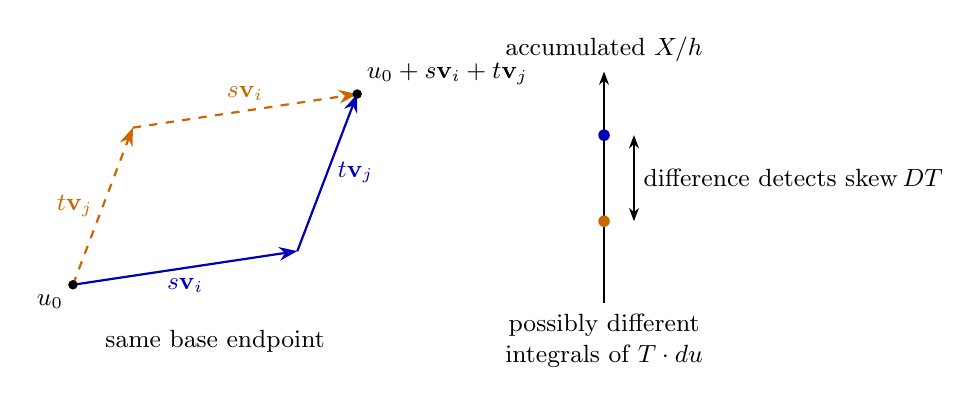
\begin{tikzpicture}[scale=0.95,>=Stealth,font=\small]
  \coordinate (O) at (0,0);
  \coordinate (A) at (3,0.45);
  \coordinate (B) at (0.8,2.1);
  \coordinate (C) at (3.8,2.55);
  \draw[->,thick,blue!70!black] (O) -- (A)
    node[midway,below] {\(s\mathbf v_i\)};
  \draw[->,thick,blue!70!black] (A) -- (C)
    node[midway,right] {\(t\mathbf v_j\)};
  \draw[->,thick,dashed,orange!80!black] (O) -- (B)
    node[midway,left] {\(t\mathbf v_j\)};
  \draw[->,thick,dashed,orange!80!black] (B) -- (C)
    node[midway,above] {\(s\mathbf v_i\)};
  \fill (O) circle (1.8pt) node[below left] {\(u_0\)};
  \fill (C) circle (1.8pt) node[above right] {\(u_0+s\mathbf v_i+t\mathbf v_j\)};
  \node at (1.9,-0.75) {same base endpoint};
  \draw[->] (7.1,-0.25) -- (7.1,2.85)
    node[above] {accumulated \(X/h\)};
  \fill[blue!70!black] (7.1,2.0) circle (2.2pt);
  \fill[orange!80!black] (7.1,0.85) circle (2.2pt);
  \draw[<->] (7.5,0.85) -- (7.5,2.0)
    node[midway,right] {difference detects \(\operatorname{skew}DT\)};
  \node[align=center] at (7.1,-0.75) {possibly different\\integrals of \(T\cdot du\)};
\end{tikzpicture}
\caption{Two orders of the same two base displacements. The difference
between their line integrals has mixed term
\(st\bigl(DT(u_0)[\mathbf v_i]\cdot\mathbf v_j-DT(u_0)[\mathbf v_j]\cdot\mathbf v_i\bigr)\).
This is a schematic illustration of the obstruction; the proof uses
\(2m\) successive legs, with the first and last \(m\) directions
forming bases.}
\label{fig:isotropic-switching}
\end{figure}

\begin{proposition}[Conservativity of the interpolated field]
\label{a05:conservativity}
In coefficient norm, or equivalently in sup norm on the required
enlarged box up to \(K\),
\[
 \|\operatorname{skew}DT\|\leq K h^{p_*-1+c_0}.
\]
\end{proposition}

\begin{proof}
Otherwise restrict to a subsequence where the skew coefficient
norm is at least \(h^{p_*-1+c_0}\).
Normalize the restored state-selected incidence measure in \(Q\)
to a probability \(\Pp\). Its mass denominator is at least
\(h\nu_Q/K\), so its base density is at most \(K\).
After discarding an arbitrarily small fraction of starting events,
the polynomial sublevel estimate gives skew at least
\(h^{p_*-1+c_0}/K\) at every retained start. A sufficiently large
subpower threshold makes this discarded mass as small as needed.

Starting from \(e_0=(l_0,t_0)\), perform \(2m\) switches.
From \(e_{i-1}\), draw \(e^\diamond=(l_i,t^\diamond)\) afresh
from \(\Pp(\,\cdot\mid\mathcal D(e_{i-1}))\).
Then retain its line and draw \(t_i\) from the conditional
\(\Pp\)-law given \(l_i\), producing \(e_i=(l_i,t_i)\).
Both operations preserve the marginal \(\Pp\).
A line with pre-normalization weighted duration below \(h/K_1\)
has \(\Pp\)-probability at most \(K/K_1\), by the full assigned
prior weight \(\nu_Q\) and the preceding mass denominator.
A union bound therefore removes short choices at arbitrarily
small path cost.

Before these longness restrictions, the velocity at each switch,
conditional on its whole past, is sampled from a prepared state
law. Its probability in any specified thin pencil is as small
as needed. Sequential avoidance therefore gives, with probability
bounded below, a well-conditioned basis from the first \(m\)
velocities and another from the last \(m\).
Take sufficiently fine bins so their centers retain the determinant
bounds. Consequently paths with a high-skew start, these two
bases, and only long choices have probability bounded below.

For every current edge and past history, the \emph{unnormalized}
next-step measure, restricted to long choices, obeys
\begin{equation}\label{a05:transition-domination}
 d\Pp\{[V_{l_i}]=J,\ t_i\in dt_i,\ l_i\text{ long}
                  \mid\text{current edge and past}\}
       \leq K\pi(J)\,\frac{dt_i}{h}.
\end{equation}
The state law supplies \(K\pi(J)\). On each long line,
\Cref{a05:incidence-density} divided by its duration bounds the
endpoint-time density by \(K/h\). We do not normalize the good
transition kernel. Iterating conditional integration backwards
therefore bounds every nonnegative function of the start,
control bins and endpoint times by \(K\) times the product
of the starting \(\Pp\)-law, the palette measures and \(dt_i/h\).
No independence after conditioning on a successful path is needed.
For fixed start, the change to signed increments
\[
 \delta_i=(t_i-t_{i-1})/h
\]
is triangular with Jacobian one in normalized times; they range
in \([-1,1]^{2m}\).

For binned control directions \(\widetilde{\bf v}_i\), simulate
base legs \(\widetilde{\bf v}_i\delta_i\) in \(u\), and simulate
increments in \(X/h\) by integrating
\(T\cdot\widetilde{\bf v}_i\) on these signed legs.
Switching within \(W_b\) introduces only \(Kb\) physical error
when the new line is evaluated at the previous time.
By \Cref{a05:line-field-comparison} and the bounded coefficients
of \(T\), the final simulation errors are
\[
 K(b/h+p_v)\ll\xi
 \quad\text{in }u,\qquad
 K(b/h+p_v+\eps_T)\ll a_1/h
 \quad\text{in }X/h,
\]
where \(p_v\) is the velocity-bin width.
The second comparison has a fixed power margin:
\[
 \eps_T/(a_1/h)\sim_{\log,N}h^{\alpha/2}.
\]

Write the endpoint map as
\[
 \delta\longmapsto
       (u_0+A\delta,\ \mathcal R(\delta)),
\]
where \(A\) has columns \(\widetilde{\bf v}_i\) and
\(\mathcal R\) is a polynomial of fixed degree.
Let \(I,J\) be the first and last \(m\) indices.
The columns in \(I\) determine every base displacement. Consequently
the derivative in a direction \(j'\in J\), minus the corresponding
combination of derivatives in \(I\), leaves the base endpoint fixed.
Its effect on the accumulated height is measured by a maximal
Jacobian minor. For \(j'\in J\), the maximal Jacobian minor using \(I\cup\{j'\}\),
divided up to sign by \(\det A_I\), equals
\[
 \partial_{j'}\mathcal R
 -(\nabla_I\mathcal R)^{\rm T}A_I^{-1}A_{j'}.
\]
Differentiate this identity at zero in each coordinate of \(I\).
If every minor had polynomial norm at most \(\eta\), the cross
Hessian would differ by at most \(K\eta\) from
\[
 A_I^{\rm T}H_{\rm sym}A_J,\qquad
 H_{\rm sym}
   =A_I^{-{\rm T}}(D^2\mathcal R(0))_{I,I}A_I^{-1},
\]
a symmetric matrix transported between the two bases.
Here fixed-degree polynomial derivative bounds control a
derivative at zero by the minor norm.
On the other hand, directly differentiating the successive
integrals gives, for \(i\in I,j'\in J\),
\[
 (D^2\mathcal R(0))_{i,j'}
       =DT(u_0)[\widetilde{\bf v}_i]\cdot
                    \widetilde{\bf v}_{j'}.
\]
Later legs have zero duration at zero, so there are no additional
cross terms. Inverting both bases bounds the skew of \(DT(u_0)\)
by \(K\eta\). Hence for the high-skew starts at least one maximal
minor has polynomial norm at least \(h^{p_*-1+c_0}/K\).

For every start and control tuple, choose such a minor and remove
the region where its absolute value is below
\(h^{p_*-1+c_0}/K_1\). Fixed-degree polynomial sublevels in
Lebesgue increments, together with
\Cref{a05:transition-domination}, make the removed path mass
arbitrarily small. On the passing region, fix the complementary
\(m-1\) increment coordinates. The regular fibers of the remaining
polynomial map have bounded multiplicity, by the fixed-degree
semialgebraic fiber bound. The change-of-variables formula thus
bounds the Lebesgue measure mapped into one endpoint cell by
\[
 K\xi^m(a_1/h)\,h^{-(p_*-1+c_0)}.
\]
The complementary coordinates have bounded volume. The resulting
cell estimate has the full \(m+1\)-dimensional volume factor
\(\xi^m(a_1/h)\). It remains to sum it over the smaller support
available to the actual endpoints.
Every actual long path has its simulated endpoint in a bounded
enlargement of the union counted by \Cref{a05:joint-support}.
Summing and integrating the start and palette weights bounds
the successful-path probability by
\[
 \begin{aligned}
 K(a/a_1)^d(a_1/h)h^{-(p_*-1+c_0)}
 &\leq K h^{e_1(1-d)-c_0}\\
 &=K h^{e_1(1-d)/2}\longrightarrow0.
 \end{aligned}
\]
This contradicts the positive lower probability and proves the
proposition.
\end{proof}

\subsection{A potential and concentrated intercept groups}

Define the polynomial
\[
 P(u)=h\int_0^1T(tu)\cdot u\,dt.
\]
Differentiating under the integral and comparing with \(hT(u)\)
leaves only the skew derivative integrated against a bounded
multiple of \(u\). Thus \Cref{a05:conservativity} gives
\begin{equation}\label{a05:potential-error}
 |\nabla P-hT|\leq Kah^{c_0}.
\end{equation}
The norms of all fixed positive derivatives of \(P\) are at
most \(Kh\) on the needed enlarged box.
For a long line in \Cref{a05:line-field-comparison},
the variation of \(X-P(u)\) across the block is at most
\(Kah^{c_0}\): integrate the directional error over time \(h\),
using \(h\eps_T\leq Kah^\alpha\) and \(c_0<\alpha\).

Bin the midpoint value of \(X-P(u)\) to width \(a_2\), denoting
its bin and center by \(C\). This is invariant along the
assigned trajectory. At a state \(\mathcal D\) of long labels,
only boundedly many neighboring \(C\)'s occur:
the variation \(Kah^{c_0}\) is much smaller than \(a_2\), the
state knows \(X,u\) much more accurately, and \(P\) has controlled
gradient.
Within one intercept group, the normalized base density, after
division by \(h\nu_Q\), is at most
\begin{equation}\label{a05:intercept-base-cap}
 K(a_2/a)^d.
\end{equation}
Indeed apply the exact-base \(X\)-cap at width \(a_2\), whose
center follows \(P(u)+C\), then use
\(\nu_Q\sim_{\log,N}a^dh^j\).

We next bound the number of groups without asserting that an
arbitrary restriction preserves breadth. First remove short
lines globally in \(Q\), and states with excessive fractional
loss. In each remaining state remove the fractions belonging
to \(C\)'s of mass below a sufficiently small fixed fraction.
There are only boundedly many \(C\)'s there, so the lost fraction
is small. Remove short lines again in this family, still with
only one \(C\) per line. Remove \((\mathcal D,C)\)-states with
excessive fractional loss, and groups with excessive total
loss compared with before the last short-line deletion.
Mass at least \(h\nu_Q/K\) remains.
If a group has remaining mass \(M\), its contributing prior
weight is at most \(KM/h\), using the immediately preceding
duration test.
At each surviving \((\mathcal D,C)\), the law is at least a
fixed fraction of the original good state law, up to the chosen
small losses. The pencil probabilities were chosen smaller
than these fractions. All needed breadth and palette bounds
therefore survive.

Apply \Cref{a05:determinant-kakeya} in dimension \(m\) to the
affine base lines of one group, in \(u\)-coordinates.
Assign \(\xi\)-cells by state centers. A line spends at most
\(Kh\xi\) weighted physical time in one such cell, and its
radius-\(O(\xi)\) tube contains the assigned cell.
If \(m_E\) are the group cell masses, determinant success and
the prior-weight bound imply
\[
 \sum_E\big((m_E/(h\xi))^m/K\big)^{1/(m-1)}
       \leq K(M/h)^{m/(m-1)}.
\]
Power mean gives at least \(K^{-1}\xi^{-m}\) occupied base cells
per group. Each joint cell at \(X\)-width \(a_2\) pays for at
most \(K\) intercept groups, since the variation of \(P\) on
a base cell is negligible compared with \(a_2\).
The count in \Cref{a05:joint-support} with \(i=2\) now yields
at most \(K(a/a_2)^d\) groups.

Delete groups below
\begin{equation}\label{a05:heavy-group}
 K^{-1}h\nu_Q(a_2/a)^d
\end{equation}
with a sufficiently large denominator. The summed loss is small.
On every retained long line in any group,
\begin{equation}\label{a05:potential-fit}
 |X_l(t)-P(u_l(t))-C|\leq Ka_2
 \quad\text{throughout the entire }Q\text{-block}.
\end{equation}
All subsequent counts use these heavy groups and their immediately
preceding long witnesses.


\subsection{Seven directions and the exceptional conic}

The remaining task is to replace the potential fit by an allowed
quadratic test. In three base variables, even directions with every
triple independent can all lie on a nonsingular conic. Third
directional tests along those directions therefore need not force
every higher-order term to vanish. We must identify the cubic and
quartic terms that survive, and later express them using the hidden
coordinate so that the final test is quadratic.

For a symmetric rank-\(r\) tensor \(T\) on \(\R^3\), associate the
homogeneous form \(F_T(x)=T(x,\ldots,x)\).
Testing \(T(p_i,p_i,p_i,\cdot,\ldots,\cdot)=0\) is equivalent to
the vanishing at \(p_i\) of all partial derivatives of \(F_T\)
of order \(r-3\), up to nonzero constants depending only on \(r\).
We call these the three-copy tests. For seven directions with
every triple independent, the following lemma identifies their
kernels. If the directions lie on a conic \(q=0\), the rank-three
and rank-four kernels are \(q\) times a linear form and a multiple
of \(q^2\), while the rank-five kernel vanishes.
The cubic two-copy test \(T(p_i,p_i,\cdot)\) has a
different role: it is injective even in the conic case and will
control the third derivatives of a branch from its differentiated
second-directional tests. The following lemmas also supply the
conditioning bounds and the passage from approximate conic
directions to exact real ones needed for those applications.

\begin{lemma}[Seven-direction tensor tests]\label{lem:tensor-kernels}
Let \(p_i=(1,v_i)\in\R^3\), \(1\leq i\leq7\), with every triple
linearly independent.
\begin{enumerate}
\item The space of homogeneous quadratics vanishing at all \(p_i\)
has dimension at most one; every nonzero member is nonsingular.
\item The map on symmetric cubic tensors
\[
 T\longmapsto\bigl(T(p_i,p_i,\cdot)\bigr)_{i=1}^7
\]
is injective.
\item If a nonzero quadratic \(q\) vanishes at all seven points,
the kernels of the three-copy tests at ranks \(3,4,5\) are,
under the homogeneous-form correspondence,
\[
 q\,(\R^3)^*,\qquad \R q^2,\qquad \{0\},
\]
respectively.
\end{enumerate}
These assertions have polynomial conditioning. More precisely, if
\[
 |p_i|\leq A,\qquad
 |\det(p_i,p_j,p_k)|\geq A^{-1},\qquad A\geq2,
\]
the inverse of the injective map in part~2 costs at most \(CA^C\).
On the exact-conic family, with the norm, inverse norm and inverse
determinant of \(q\) also bounded by fixed powers of \(A\),
distance to each kernel in part~3 is at most \(CA^C\) times
the norm of the corresponding tests. The constants depend only
on these fixed finite-dimensional spaces and on the fixed
conditioning powers.
\end{lemma}

\begin{proof}
All divisibility arguments can be made over \(\C\).
A complex line contains at most two of the seven points, since
three real linearly independent vectors are also complex linearly
independent. A singular projective conic, being a union of two
lines with multiplicity allowed, cannot contain five of them.

There is exactly one conic through any five, up to scalar.
Indeed, use the first three points as a projective coordinate
basis. Quadratics vanishing there have form
\(a x_0x_1+b x_0x_2+c x_1x_2\).
The remaining two points have all coordinates nonzero.
Their vectors \((x_0x_1,x_0x_2,x_1x_2)\) are not proportional,
since their ratios recover the projective point.
They give two independent conditions on \((a,b,c)\).
Thus the five-point conic space is one-dimensional, and its
nonzero member is nonsingular by the preceding paragraph.
Part~1 follows.

If \(T(p_i,p_i,\cdot)=0\) for a cubic form \(F\), all its
first partial derivatives belong to that quadratic space.
If the space is zero, \(F=0\). Otherwise write
\(\partial_jF=c_jq\). Euler's identity yields \(F=qL\)
for a linear form \(L\). At every tested point,
\[
 0=\nabla F(p_i)=L(p_i)\nabla q(p_i).
\]
Nonsingularity gives \(L(p_i)=0\), and three independent points
force \(L=0\). This proves part~2.

A cubic vanishing at seven distinct points of a nonsingular
conic is divisible by its equation. Here is an elementary
justification of this intersection fact. Over \(\C\), change
coordinates to write the conic as \(x_0x_2-x_1^2=0\), with
parametrization
\([s:t]\mapsto[s^2:st:t^2]\).
The restriction of a cubic is a binary sextic; seven distinct
projective zeros make it identically zero.
For any homogeneous degree, reduction modulo \(x_0x_2-x_1^2\)
leaves monomials using no pair \(x_0,x_2\) simultaneously.
Their substitutions are distinct binary monomials, with the
common monomial \(x_1^r\) counted once. Thus a zero restriction
has zero remainder, proving divisibility.
The rank-three kernel is therefore exactly \(q\) times the
linear forms.

For a quartic \(F\) in the rank-four kernel, each first partial
derivative is such a cubic and is divisible by \(q\).
Euler gives \(F=qH\), with \(H\) quadratic. Then
\[
 \partial_jF=(\partial_jq)H+q\partial_jH.
\]
Choose a nonzero linear partial derivative of \(q\).
The irreducible quadratic \(q\) is relatively prime to it,
so divisibility of \(\partial_jF\) by \(q\) forces \(q\mid H\).
Hence \(F\) is a multiple of \(q^2\).
Conversely, \(q^2\) and its first derivatives vanish at the
seven points.

For a quintic in the rank-five kernel, every second derivative
is a cubic divisible by \(q\). Each first derivative consequently
satisfies the preceding quartic test and is a multiple of \(q^2\).
Euler gives \(F=q^2L\) with \(L\) linear.
Differentiation and reduction modulo \(q^2\) force
\(q\mid(\partial_jq)L\), and hence \(q\mid L\) for a nonzero
partial derivative. Therefore \(L=0\).
This proves all kernel equalities.

For fixed \(A\), the point configurations form a compact
semialgebraic set. The matrix of the cubic two-copy test has
polynomial entries and is injective everywhere on this set,
so its least singular value has a positive minimum.
For the three-copy tests restrict to the compact exact-conic
family, imposing the stated coefficient and determinant bounds.
Their kernel dimensions are constantly \(3,1,0\), so their
least positive singular values also have positive minima.
The minima are semialgebraic functions of \(A\), by real
quantifier elimination; orthogonality to a kernel and unit norm
are fixed-format polynomial conditions.

A positive semialgebraic function of one real parameter has a
reciprocal polynomial lower bound at infinity.
To see the rate relevant here, decompose its graph into finitely
many algebraic branches for large \(A\). On each, a nonzero
relation \(P(A,s)=0\) holds. Remove powers of \(s\) from \(P\).
Its constant coefficient in \(s\) is then a nonzero polynomial
in \(A\), bounded below by a power of \(A\) for large \(A\);
all other coefficients are bounded above by powers of \(A\).
For \(0<s\leq1\), the relation forces \(s\geq cA^{-C}\).
Absorb bounded parameter intervals into the constant.
The claimed inverse estimates follow. Crucially the rank-four
estimate is applied on the exact-conic family: its rank can
increase when the points move off that family.
\end{proof}

\begin{lemma}[Restoration of an approximate real conic]
\label{a05:real-conic}
Suppose the points satisfy the conditioning bounds of
\Cref{lem:tensor-kernels}, and a real quadratic \(q(x)=x^{\rm T}
\mathsf Qx\) has
\(A^{-1}\leq\|q\|\leq A\) and \(|q(p_i)|\leq\epsilon\).
If \(\epsilon\) is smaller than a sufficiently large fixed
reciprocal power of \(A\), then
\[
 |\det\mathsf Q|\geq cA^{-C},
\]
and there are exact real zeros \(p'_i=(1,v'_i)\) of \(q\) with
\[
 |p'_i-p_i|\leq CA^C\epsilon.
\]
For sufficiently small \(\epsilon\), every triple determinant
of the shifted points has absolute value at least \((2A)^{-1}\).
\end{lemma}

\begin{proof}
For coefficient-normalized quadratics the function
\[
 |\det\mathsf Q|+\sum_{i=1}^7|q(p_i)|
\]
has a positive minimum on the compact point family:
a zero would be a nonzero singular quadratic through all seven
points, contrary to \Cref{lem:tensor-kernels}.
The semialgebraic argument in that lemma gives a lower bound
\(cA^{-C}\). Normalize the given \(q\), use the smallness of
its evaluations, then rescale to obtain the determinant bound.

It bounds the smallest singular value of \(\mathsf Q\) below
by \(cA^{-C}\), and hence the homogeneous gradient at each
\(p_i\) below by such a bound. Write
\(g_i=\nabla_vq(1,v_i)\).
Euler's identity reads
\[
 \partial_0q(1,v_i)+v_i\cdot g_i=2q(1,v_i).
\]
Since \(|v_i|\leq A\) and \(q(1,v_i)\) is sufficiently small,
the full-gradient bound implies \(|g_i|\geq cA^{-C}\).
With \(e_i=(0,g_i/|g_i|)\),
\[
 q(p_i+te_i)=q(p_i)+|g_i|t+b_it^2,\qquad |b_i|\leq CA.
\]
If \(q(p_i)\ne0\), take \(t=-2q(p_i)/|g_i|\).
For sufficiently small \(\epsilon\), the quadratic term has
absolute value below \(|q(p_i)|/2\), so this value has the
opposite sign from \(q(p_i)\).
The intermediate value theorem gives a real zero at distance
at most \(2|q(p_i)|/|g_i|\). If \(q(p_i)=0\), no shift is needed.
The first coordinate remains one. Multilinearity shows that
triple determinants change by at most
\(CA^2\max_i|p_i'-p_i|\), proving the final assertion.
\end{proof}

\subsection{Restoring quadratic tests}

\begin{proposition}[Degree restoration]\label{prop:degree-restoration}
The potential fits and heavy intercept groups constructed above
yield a candidate with all the properties in
\Cref{thm:isotropic-improvement}, without reducing the
positive exponent \(e_2\) in \(a_2/a=h^{e_2}\).
\end{proposition}

\begin{proof}
We treat the two versions separately.
\paragraph{Version~1.}
Choose a heavy intercept group. In normalized block time,
\Cref{a05:potential-fit} compares \(P\) with the quadratic
\(X-C\) along each of its lines. Polynomial Remez gives
\[
 |D_{\bf v}^3P|\leq Ka_2
\]
there. Conditional product sampling and palette averaging fix
four separated very fine velocity bins with witnesses on common
states carrying an inverse-subpower fraction of the group.
Use their centers as directions. The locations in a state
differ by at most \(Kb/h\) in \(u\), and fixed derivatives of
\(P\) cost \(Kh\). Finer velocity bins and \(b/h\ll a_2/h\)
make the transferred errors negligible.
By \Cref{a05:heavy-group,a05:intercept-base-cap}, these common
tests hold on inverse-subpower base volume.
Polynomial Remez extends them to the enclosing box.
A binary cubic is determined by its values in four separated
directions \((1,V_i)\); inversion of this Vandermonde system
costs \(K\). Hence \(\|\nabla^3P\|\leq Ka_2\).
The quadratic Taylor polynomial of \(P+C\) fits to \(Ka_2\)
on the block box. The test \(w\) minus this polynomial has hidden
derivative one and zero hidden curvature, and its heavy-group
mass is the required one.

\paragraph{Branches in version~2.}
Here \(w\) may be uncontrolled in tangent units, so we use the
native test rather than assume a bound for \(w\).
In each heavy group consider
\begin{equation}\label{a05:branch-equation}
 P_*(z,w)=P(u)+C,\qquad z=z_c+hu.
\end{equation}
At path observations the residual is \(O(Ka_2)\), the absolute
hidden derivative lies between \(K^{-1}\) and \(K\), and the
hidden curvature is at most \(K\).
The discriminant expression
\[
 \Delta(u)
 =(P_{*,w})^2
       -2P_{*,ww}\bigl(P_*(z,w)-P(u)-C\bigr)
\]
is independent of \(w\), because the equation is quadratic in
\(w\) with constant quadratic coefficient.
It lies between \(K^{-1}\) and \(K\) on the observations.
The heavy-group floor divided by
\Cref{a05:intercept-base-cap} gives inverse-subpower base
volume. Polynomial Remez bounds the coefficients and derivatives
of \(\Delta\) on an enlarged complex box by \(K\).
Thus, about every used point, \(\Delta\) is zero-free on a
complex ball of inverse-subpower radius with a fixed margin.

Each observed \(w_l\) is within \(Ka_2\) of a real simple root
of \Cref{a05:branch-equation}. For a quadratic, choose the root
with the same derivative sign as at \(w_l\); the derivative on
the intervening segment has size at least \(K^{-1}\), after
enlarging \(K\), by the positive discriminant and small residual.
For a linear equation, divide by its nonzero coefficient.
The roots extend holomorphically to the stable balls, by a
holomorphic square root of \(\Delta\), or by linear division.

Choose a lattice of real comparison cores, each inside a
fixed several-fold complex enlargement, with radius common
up to \(K\) among the groups. Assign a core by the
\((\mathcal D,C)\)-center. Since \(Kb/h\) is negligible, it
contains the state's used points with an interior margin.
Boundary points can be assigned in a bounded overlapping cover.
Add the sign of the nearby root.
Discard sign fractions smaller than a sufficiently small fixed
fraction; the core choice itself removes no fraction at a state.
Delete line/intercept/core/sign portions with weighted duration
below \(h/K_1\). Each line has one intercept and at most \(K\)
core/sign choices, so the total loss is at most
\(Kh\nu_Q/K_1\). Remove states with excessive fractional loss.
The fixed-fraction comparisons to the earlier good state laws,
with sufficiently small initial pencil probabilities, retain
general position and palette domination.

There are at most \(K(a/a_2)^d\) group/core/sign choices.
One choice therefore has mass at least
\begin{equation}\label{a05:branch-mass}
 K^{-1}h\nu_Q(a_2/a)^d.
\end{equation}
Let \(U\) be its real inner ball and \(f\) its branch.
Every contributing line has an immediately preceding witness
set, in this same choice, of ordinary length at least \(h/K\),
including its currently counted incidences.
All witnesses lie in \(U\), with \(f\) holomorphic on a
sufficient complex enlargement. The convex cores and that
margin ensure that the line chords used below stay in the
controlled domain.

\paragraph{Analytic estimates before tensor inversion.}
Set
\begin{equation}\label{a05:normalized-test}
 R(u)=P_s(z_c+hu,f(u))/a.
\end{equation}
We will apply the two-copy cubic test to \(\nabla^3f\) and the
three-copy tests to the higher derivatives of \(R\). First we
need analytic bounds on \(R\) that hold before moving any
directions to an exact conic.
At the earlier witnesses, the true packet test obeys
\[
 |P_s(z,w_l)|\leq Ka,\qquad
 |P_{s,w}(z,w_l)|\leq K,\qquad
 |P_{s,ww}|\leq K/a,
 \qquad |w_l-f(u)|\leq Ka_2.
\]
Its exact quadratic Taylor formula in \(w\) gives
\[
 |R(u)|\leq K\bigl(1+a_2/a+(a_2/a)^2\bigr)\leq K.
\]
The base density of this choice is bounded by the original
group ceiling \(Kh\nu_Q(a_2/a)^d\).
Together with \Cref{a05:branch-mass}, this gives real projection
volume at least \(K^{-1}\).
The function \(R\) is holomorphic algebraic of bounded relation
degree. \Cref{lem:algebraic-norm} bounds its norm and every
required fixed derivative by \(K\) on the used interiors,
before any tensor inversion.

Along a contributing line, compare \(f\) with the affine hidden
trajectory \(w_l\), and compare \(R\) with the quadratic
\(P_s(z,w_l)/a\), on its earlier long witness set.
Normalized time on its chord has length at least \(K^{-1}\);
the witness set has inverse-subpower relative length and the
chord has the stated complex margin.
The one-variable algebraic norm bound yields, at the incidences,
\begin{equation}\label{a05:directional-branch}
 |D_{\bf v}^2f|\leq Ka_2,\qquad
 |D_{\bf v}^3R|\leq Ka_2/a.
\end{equation}

Let
\[
 S_0=\inf_{L\ {\rm affine}}\|f-L\|_{C^0(U)}.
\]
For \(S_0>0\), apply \Cref{lem:algebraic-norm} to
\(f-L\) with \(\|f-L\|_{C^0(U)}\leq2S_0\).
All fixed derivatives of order at least two are bounded by
\(KS_0\) on a slightly larger interior. If \(S_0=0\), \(f\)
is affine and these derivatives vanish.

Sample seven velocities in each retained state, sequentially
avoiding all preceding points and joining lines. The prepared
breadth gives a positive probability that all triple determinants
of \({\bf v}_i=(1,v_i)\) have size at least \(K^{-1}\).
Palette domination turns this into a product-palette mass at
least \(K^{-1}\) of eligible bin tuples. Averaging fixes one
tuple with common directional witnesses on states carrying an
inverse-subpower fraction of the current mass.
Using fine bin centers transfers their tests to actual base
points in those states. For \(R\), its preceding derivative
bounds make all mesh errors negligible relative to \(a_2/a\).
For \(f\), the Hessian and higher derivative errors are bounded
by \(KS_0\) times the normalized position and velocity errors.
Choose those errors at most \(h^2/K\), independently of \(S_0\).
Common-state mass and the base ceiling again give base volume
at least \(K^{-1}\). Apply \Cref{lem:algebraic-norm} to the
directional derivative functions themselves; differentiation
of the simple root preserves bounded algebraic relation degree
on the stable domain.
We obtain throughout \(U\), also after the fixed further
differentiations needed below,
\begin{equation}\label{a05:seven-tests}
 |D_{{\bf v}_i}^2f|\leq K(a_2+S_0h),\qquad
 |D_{{\bf v}_i}^3R|\leq Ka_2/a.
\end{equation}
The weaker \(S_0h\) allowance absorbs the \(S_0h^2\) transfer
error and subpower losses.
All ball radii and margins here cost only \(K\).

Differentiate the first tests once and apply the injective
cubic two-copy test in \Cref{lem:tensor-kernels}. Its polynomial
conditioning is subpower, so
\begin{equation}\label{a05:third-f}
 \|\nabla^3f\|\leq K(a_2+S_0h).
\end{equation}
If \(S_0\leq a_2/h\), a quadratic Taylor polynomial \(f_2\)
approximates \(f\) on \(U\) within \(Ka_2\).
The test \(w-f_2((z-z_c)/h)\) is quadratic in parent variables,
has derivative one and curvature zero, and fits the long
witnesses. This includes \(S_0=0\).

\paragraph{The conic case.}
Suppose \(S_0>a_2/h\).
Let \(u_c\) be the ball center and \(L'\) the affine Taylor
polynomial of \(f\) there. Define
\[
 q(x)=\frac{1}{2S_0}\nabla^2f(u_c)[x,x].
\]
Taylor's theorem and \Cref{a05:third-f} give
\begin{equation}\label{a05:f-conic}
 \frac{f(u)-L'(u)}{S_0}
       =q(u-u_c)+O(Kh).
\end{equation}
The relative derivative bound gives \(\|q\|\leq K\).
Conversely the definition of \(S_0\) yields
\[
 1\leq \|q\|_{C^0(U-u_c)}+Kh\leq K\|q\|+Kh,
\]
so \(\|q\|\geq K^{-1}\).
The Hessian tests imply \(|q({\bf v}_i)|\leq Kh\).
Choose one parameter \(A=N^{o(1)}\) controlling all coefficient
norms, direction sizes, and inverse triple determinants.
Since \(h\) is a fixed negative power, \Cref{a05:real-conic}
applies. It gives a determinant lower bound \(K^{-1}\) for
\(q\), and exact real zeros \({\bf v}'_i=(1,v_i')\) with
\[
 |{\bf v}'_i-{\bf v}_i|\leq Kh,
 \qquad
 |\det({\bf v}'_i,{\bf v}'_j,{\bf v}'_k)|\geq K^{-1}.
\]
Thus even a nearly singular or nearly definite proposed
quadratic is quantitatively controlled before inversion.

The independent derivative bounds for \(R\) from
\Cref{a05:normalized-test} show that these shifts alter its
rank-three, rank-four and rank-five contractions by at most
\(Kh\). This is negligible compared with
\(a_2/a=h^{e_2}\), because \(e_2<1\).
The differentiated tests in \Cref{a05:seven-tests} therefore
remain \(Ka_2/a\) in the shifted directions.
Apply the exact-conic kernels of \Cref{lem:tensor-kernels}.
The fifth derivatives of \(R\) are bounded by \(Ka_2/a\);
at \(u_c\), the cubic and quartic Taylor tensors are within
\(Ka_2/a\) of \(q\) times a linear form and a multiple of
\(q^2\), respectively. Taylor expansion through degree four gives
\begin{equation}\label{a05:R-restoration}
 R(u)=R_2(u)+q(u-u_c)L_1(u)
                +\lambda_0q(u-u_c)^2+O(Ka_2/a),
\end{equation}
where \(R_2\) is quadratic, \(L_1\) is affine, and all displayed
coefficients are bounded by \(K\).
To justify division in these factors, the coefficient norm of
a product of polynomials of fixed degrees is bounded below by
a positive constant times the product of their coefficient
norms. Normalize the factors and use compactness and the
absence of zero divisors. Since \(\|q\|\geq K^{-1}\), division
by \(q\) or \(q^2\) costs only \(K\).
A constant term of \(L_1\) can be absorbed into \(R_2\).

On the earlier long witnesses, put
\[
 H'(u,w)=\frac{w-L'(u)}{S_0}.
\]
Because \(a_2/S_0<h\), \Cref{a05:f-conic} and
\(|w-f(u)|\leq Ka_2\) imply
\(H'=q(u-u_c)+O(Kh)\) and \(|H'|\leq K\).
Define
\begin{equation}\label{a05:new-test}
 P_{\rm new}(z,w)
 =P_s(z,w)
   -a\left(R_2(u)+H'(u,w)L_1(u)
                         +\lambda_0H'(u,w)^2\right),
 \qquad u=(z-z_c)/h.
\end{equation}
Every term has total degree at most two in \((z,w)\):
\(u,H',L'\), and \(L_1\) are affine in the indicated variables.
Substituting \(H'\) for \(q\) costs \(Kah\), which is below
\(a_2\) by \(h^{1-e_2}\).
Replacing \(f\) by the actual \(w\) in \(P_s\) costs at most
\[
 K|w-f|+(K/a)|w-f|^2
       \leq Ka_2+Ka_2^2/a\leq Ka_2.
\]
Together with \Cref{a05:R-restoration}, this proves the
\(Ka_2\) value bound on the long witnesses.

The exact derivative perturbations are
\[
 \partial_w\bigl(P_s-P_{\rm new}\bigr)
       =\frac a{S_0}(L_1+2\lambda_0H'),\qquad
 \partial_{ww}\bigl(P_s-P_{\rm new}\bigr)
       =\frac{2a\lambda_0}{S_0^2}.
\]
Consequently
\begin{align}
 \bigl|\partial_w(P_s-P_{\rm new})\bigr|
   &\leq K a/S_0
     <K h^{1-e_2}\ll K^{-1},\label{a05:derivative-margin}\\
 |\partial_{ww}P_{\rm new}|
   &\leq K/a+K a/S_0^2
     \leq K/a_2+(K/a_2)h^{2-e_2}
     \leq K/a_2.\label{a05:curvature-margin}
\end{align}
The old derivative lower bound at the counted observations
survives \Cref{a05:derivative-margin}; the upper bound holds
on the earlier witnesses. No magnitude bound for \(w\),
\(L'\), or \(S_0\) was used, only the normalized value \(H'\)
and the displayed lower bound on \(S_0\).

\paragraph{The same time block.}
In both cases the test is an allowed quadratic.
On each contributing version~2 trajectory, \(z(t)\) and \(w(t)\)
are affine, so its value is a polynomial of degree at most two
in time and its hidden derivative has degree at most one.
The earlier witness set has physical length at least \(h/K\)
inside the same \(h\)-length \(Q_s\)-block.
After normalizing that block to unit length, polynomial Remez
costs only \(K\). Thus the value and derivative upper bounds
hold throughout this block. The lower derivative is needed
only on the counted incidences and was proved there.
Curvature is constant in \(w\) for these quadratic tests.
The version~1 comparison has the same fixed-degree time property.
Extrapolation is never made from an \(h/K\)-set to a unit
\emph{parent} time interval.

The retained choice has mass
\(h\nu_Q(a_2/a)^d/K\), by \Cref{a05:branch-mass} or the heavy
intercept floor in version~1. Degree restoration makes no
further discard. Dividing by its time length \(h\) gives
\(\nu_Q(a_2/a)^d/K\), exactly the candidate mass requirement.
\end{proof}

\begin{proof}[Conclusion of \Cref{thm:isotropic-improvement}]
Start with any substantial residual of the reference path.
The physical estimates and \Cref{a05:velocity-graph} retain a
substantial reference family. \Cref{a05:qualification} is an
assertion of relative \(o(1)\) failure under its frozen
post-renewal incidence law. It follows by finding qualifying
occurrences in every hypothetical substantial fixed-tolerance
failure set and then taking the slow diagonal.
The fixed-threshold deletion in \Cref{a05:good-state-deletion}
therefore leaves substantial good-state mass. Cartesian
interpolation selects a packet and states of mass
at least \(h\nu_Q/K\), then restores their prepared reference
edges. The conservativity estimate yields the potential and
heavy intercept groups constructed above; \Cref{prop:degree-restoration}
provides the required quadratic candidate. By
\Cref{a05:improvement-scales}, its gain has positive limit
\(e_2ks\). All meshes and degree bounds used to discover it
depend on fixed exponents, while the actual output construction
and its original-scale guards are those of
\Cref{prop:candidate-upgrade}. The criterion therefore gives
the isotropic contradiction on every substantial residual.
\end{proof}

\begin{corollary}[Zero horizon in the scalar model]
\label{a05:scalar-zero-horizon}
For every fixed admissible choice of angular parameters and every
\(d<1\), a version~1 exact problem in \(C(d)\) has
\(H(E)=0\). In particular there is no bad problem in version~1.
\end{corollary}

\begin{proof}
If a bad version~1 problem existed, the critical-path construction
of \Cref{prop:critical-path} would give a tangent problem with
positive \(k\) and precisely the version~1 data above.
\Cref{thm:isotropic-improvement,prop:candidate-upgrade} would
contradict its maximizing-path exclusion.
\end{proof}

This scalar conclusion is established before the finite-narrowness
analysis. It supplies the version~1 input to
\Cref{thm:scalar-mesh-projection}, whose projection labels are then
used in \Cref{sec:finite-narrowness,sec:critical-rates,sec:unbounded-narrowness}.
The unbounded-narrowness case retains its separate limiting construction.

\section{Retained-edge planar tools}\label{sec:retained-edge-tools}

We prove that a row whose evaluation is nearly constant along many
lines agrees, on many incidences, with a constant row plus a multiple
of \(Jz\), where \(J(t,Z)=(-Z,t)\).  This is
\Cref{a06:row-fit}, used in both the finite-narrowness reduction and
the critical-rate argument.

The main step is planar rigidity for graphs with small restricted
sumsets: many original edges have their endpoints in two parallel
strips, of width equal to the mesh up to a subpower factor and with
subpower-bounded common slope.  Keeping original edges allows this
geometric conclusion to be lifted back to incidence mass.  We first
prove the planar statement, then apply it to the line projections
that arise from the row.

Throughout this section \(h=N^{-a}\), where \(a>0\) is fixed, and
\(K=h^{-o(1)}\) may increase by a fixed power from line to line.
For a bounded planar set \(U\), \(N_h(U)\) is its covering number by
squares of side \(h\).  Fixed-grid and separated-set versions differ
only by dimensional constants.  Constants indexed by a fixed
expression length may depend on that length, but remain subpower in
\(h^{-1}\).  The final passage to strip widths \(h^{1-o(1)}\) uses
a slow diagonal and may introduce a new subpower factor.

\subsection{Graph refinement and common endpoint sets}

We begin with the graph form of Balog--Szemer\'edi--Gowers that records
the edges surviving the sumset reduction. The three-path argument
follows \citet[Lemma~4.2 and the proof of Theorem~4.1]{SudakovSzemerediVu2005}; compare also
\citet[Theorem~2.29 and Exercise~6.4.10]{TaoVu2006} for the graph
form and retention of original edges. We give the proof with the
polynomial dependence needed after mesh rounding.

\begin{lemma}[Three paths retain graph edges]\label{re:graph-bsg}
Let \(A,B\) be nonempty finite subsets of an abelian group, with
\(a_0=|A|\), \(b_0=|B|\), and let \(G\subset A\times B\) have at least
\(\theta a_0b_0\) edges, \(0<\theta\le1\).  Put
\(C=\{x+y:(x,y)\in G\}\).  There are \(A'\subset A\), \(B'\subset B\)
such that
\begin{align*}
 |A'|&\ge c\theta a_0,\qquad |B'|\ge c\theta b_0,\\
 |G\cap(A'\times B')|&\ge c\theta^2a_0b_0,\qquad
 |A'+B'|\le C_0\theta^{-5}\frac{|C|^3}{a_0b_0},
\end{align*}
where \(c,C_0>0\) are absolute constants.
\end{lemma}
\begin{proof}
We first choose endpoint sets with many three-edge walks between every
pair.  The sums along those walks will bound the full sumset, while
degree counting will retain many edges of the original graph.
Remove vertices of \(A\) of degree below \(\theta b_0/2\), retaining
a set \(A_0\) and at least \(\theta a_0b_0/2\) edges.  An ordered pair
in \(A_0^2\) is bad if its common neighborhood has fewer than
\(\tau b_0\) vertices, where \(\tau=\theta^3/512\).  For uniform
\(v_0\in B\) let \(U=N(v_0)\cap A_0\).  Degree counting and Jensen give
\[
 \E|U|\ge\theta a_0/2,\qquad
 \E|U|^2\ge\theta^2a_0^2/4,\qquad
 \E\operatorname{Bad}(U)\le\tau a_0^2,
\]
the last bound because a bad pair has probability below \(\tau\) of
lying in \(U^2\).  For one \(U\), therefore,
\[
 |U|^2-(32/\theta)\operatorname{Bad}(U)
 \ge 3\theta^2a_0^2/16.
\]
It follows that \(|U|\ge\theta a_0/(2\sqrt2)\) and
\(\operatorname{Bad}(U)\le\theta|U|^2/32\).  Delete vertices having
more than \(\theta|U|/16\) bad partners.  At most half of \(U\) is
deleted; call the remainder \(A'\).  Define
\[
 B'=\{v\in B:|N(v)\cap A'|\ge\theta|A'|/4\}.
\]
Every member of \(A'\) retains degree at least \(\theta b_0/2\) in
the original graph.  Edges to \(B\setminus B'\) number at most
\(\theta|A'|b_0/4\), so
\[
 |G\cap(A'\times B')|\ge\theta|A'|b_0/4,
 \qquad |B'|\ge\theta b_0/4.
\]

Fix \(u\in A'\) and \(v\in B'\).  Of the at least
\(\theta|A'|/4\ge\theta|U|/8\) vertices in \(N(v)\cap A'\), at most
\(\theta|U|/16\) form a bad pair with \(u\).  Each remaining \(u_1\)
has at least \(\tau b_0\) common neighbors \(v_1\) with \(u\).
Thus \(u,v\) have at least \(c\theta^5a_0b_0\) original-graph walks
\(u,v_1,u_1,v\).  The walk determines
\[
 (u+v_1,\ u_1+v_1,\ u_1+v)\in C^3,
\]
and, for fixed \(u,v\), this map is injective.  Its alternating sum
is \(u+v\).  Choose one representing pair for every distinct element
of \(A'+B'\); the corresponding triples are disjoint.  Hence
\(c\theta^5a_0b_0|A'+B'|\le |C|^3\), as required.
\end{proof}

Here is the common finite-mesh input for the next three lemmas.  The
parameter law may be a law on indices: distinct direction bins with the
same rounded parameter are not silently identified.  The graph bounds
refer to the corresponding original edge sets.

\begin{assumption}[Planar graph data]\label{re:graph-data}
Let \(A,B\subset h\Z^2\cap[-K,K]^2\), with
\(h^{-1}/K\le |A|,|B|\le Kh^{-1}\).  A probability law \(\nu\) on
represented indices \(\kappa\) obeys, for a fixed \(S>0\),
\begin{equation}\label{re:ratio-cap}
 K^{-1}\le|\kappa|\le K,\qquad
 \nu(I)\le K|I|^S\quad(h\le |I|\le1).
\end{equation}
For each index there is \(G_\kappa\subset A\times B\) with
\begin{equation}\label{re:graph-hypotheses}
 |G_\kappa|\ge h^{-2}/K,\qquad
 N_h\{x+\kappa y:(x,y)\in G_\kappa\}\le Kh^{-1}.
\end{equation}
The uniform law on \(G_\kappa\) obeys, for intervals \(I,I'\) of
length \(h\),
\begin{equation}\label{re:first-coordinate-cap}
 \Pp(x_1\in I,y_1\in I')\le Kh^2.
\end{equation}
\end{assumption}

Set \(L=h^{-1}\) in this section.  For each \(\kappa\), round
\(A\) and \(\kappa B\) to \(h\Z^2\).  Since \(|\kappa|\) and its
reciprocal are subpower, a rounded vertex has at most \(K\)
preimages, after increasing \(K\); an image edge has at most \(K^2\)
preimages.  The image graph therefore has subpower density, while
the set of its edge sums has at most \(KL\) rounded values.
Apply \Cref{re:graph-bsg} to this image graph and pull back all
preimages of the selected vertices.  Every retained image edge has
an original preimage, so the result is not merely a vertex-set
statement.  We obtain \(A_\kappa\subset A\), \(B_\kappa\subset B\)
such that
\begin{equation}\label{re:individual-bsg}
 |A_\kappa|,|B_\kappa|\ge L/K,\qquad
 N_h(A_\kappa+\kappa B_\kappa)\le KL,\qquad
 |G_\kappa\cap(A_\kappa\times B_\kappa)|\ge L^2/K.
\end{equation}

We use the covering-number forms of the Ruzsa triangle and fixed-iterate
Pl\"unnecke--Ruzsa inequalities \citep{TaoVu2006}:
\begin{align}
 N_h(U-W)N_h(V)&\le C N_h(U-V)N_h(V-W),
 \label{re:ruzsa-triangle}\\
 N_h(mU-nU)&\le C_{m,n}K^{C_{m,n}}N_h(U)
 \quad\text{if }N_h(U-U)\le K N_h(U).
 \label{re:iterate}
\end{align}
These apply to \(h\)-cell unions after rounding, with only fixed
dimensional changes of mesh.  For the first inequality, choose one
representing pair for each separated output \(u-w\) and let \(v\)
range over a separated subset of \(V\); the rounded pair
\((u-v,v-w)\) determines both the output and \(v\), up to bounded
choices.  We also use the elementary covering lemma
\begin{equation}\label{re:covering}
 N_h(U+V)\le K N_h(V)
 \quad\Longrightarrow\quad
 U\subset\bigcup_{i=1}^{CK}(u_i+V-V+B(0,Ch)).
\end{equation}
To see this, take a maximal disjoint collection of translates of
\(V+B(0,h)\) inside \(U+V+B(0,h)\); volume comparison bounds their
number and maximality gives the inclusion.

The sets in \eqref{re:individual-bsg} depend on the parameter.  We next
choose one pair of endpoint sets that has large overlap with the sets
for many parameters.  The Ruzsa inequalities then control sums of
fixed numbers of dilates of this one pair, including the scalar
expressions needed later in the collision argument.

\begin{lemma}[A common pair and scalar closure]\label{re:common-sets}
After restricting \(\nu\) to a subpower fraction of its mass, there
are a represented \(\kappa_0\), fixed \(A_*\subset A\), \(B_*\subset B\),
and \(\mathcal R=\{\kappa/\kappa_0\}\) with the following properties.
At least \(L^2/K\) original edges of \(G_{\kappa_0}\) lie in
\(A_*\times B_*\).  Put \(E=A_*\), \(F=-\kappa_0B_*\).
For every fixed \(m,H\), the set
\begin{equation}\label{re:scalar-support}
 c_1E+\cdots+c_mE+d_1F+\cdots+d_mF
\end{equation}
has at most \(K_{m,H}L\) \(h\)-cells whenever each coefficient is a
sum of at most \(H\) signed products of at most \(H\) elements of
\(\mathcal R\).  A common subpower dilation of all coefficients is
permitted.  The restricted probability law on \(\mathcal R\) still
satisfies a bound of the form \eqref{re:ratio-cap}, with a new
subpower constant and the same fixed exponent \(S\).
\end{lemma}
\begin{proof}
The rectangles \(A_\kappa\times B_\kappa\) from
\eqref{re:individual-bsg} sit in the one universe \(A\times B\),
which has at most \(K^2L^2\) elements.  Independent indices satisfy
\[
 \E_{\kappa,\kappa'}
 |(A_\kappa\times B_\kappa)\cap
   (A_{\kappa'}\times B_{\kappa'})|
 \ge\frac{(\E_\kappa|A_\kappa\times B_\kappa|)^2}{|A\times B|}
 \ge L^2/K^6.
\]
Choose \(\kappa_0\) with at least this average intersection, then
retain indices with intersection at least \(L^2/(2K^6)\).  Their
probability is at least \(1/(2K^8)\).  Set
\(A_*=A_{\kappa_0}\), \(B_*=B_{\kappa_0}\).  Because each
individual set has at most \(KL\) points, the retained indices have
\[
 |A_\kappa\cap A_*|,\ |B_\kappa\cap B_*|\ge L/(2K^7).
\]
The edge assertion follows from \eqref{re:individual-bsg} at
\(\kappa_0\).  Restricting and renormalizing the index law costs only
a subpower factor in its interval bound; division by
\(\kappa_0\), whose norm and reciprocal are subpower, does likewise.

For clarity about the uniform set calculus, put
\[
 d_h(U,V)=\log\frac{N_h(U-V)}{\sqrt{N_h(U)N_h(V)}}.
\]
The triangle inequality \eqref{re:ruzsa-triangle} is the triangle
inequality for \(d_h\), up to \(O(1)\).  Changing mesh from \(h\)
to \(h/K^C\), or dilating both sets by a scalar with norm and
reciprocal at most \(K^C\), changes the bounds below by \(O_C(\log K)\):
a planar cell refines into at most \(O(K^{2C})\) cells.
The small cross sum in \eqref{re:individual-bsg} gives
\(d_h(A_\kappa,-\kappa B_\kappa)=O(\log K)\).  Applying the triangle
inequality in both directions gives small self-differences for
\(A_\kappa\) and \(B_\kappa\).  To use the large intersections,
put \(H_\kappa=A_\kappa\cap A_*\).  Both
\(A_\kappa-H_\kappa\) and \(H_\kappa-A_*\) are contained
in the corresponding self-difference sets.  Since
\(|H_\kappa|\ge L/(2K^7)\), the triangle inequality through
\(H_\kappa\) gives \(d_h(A_\kappa,A_*)=O(\log K)\).
The same argument for the intersections of the \(B\)-sets gives
\(d_h(B_\kappa,B_*)=O(\log K)\).  Consequently
\begin{equation}\label{re:fixed-cross}
 d_h(E,F)=O(\log K),\qquad
 d_h(E,tF)=O(\log K)\quad(t\in\mathcal R).
\end{equation}
Here the second relation uses \(tF=-\kappa B_*\).
To transfer this relation from \(F\) to \(E\), use the triangle
inequality through \(tF\) and then undo the common dilation:
\begin{align*}
 d_h(E,tE)
 &\le d_h(E,tF)+d_h(tF,tE)+O(1)\\
 &=d_h(E,tF)+d_h(F,E)+O(\log K)
 =O(\log K).
\end{align*}
The dilation error is uniform because both \(|t|\) and
\(|t|^{-1}\) are subpower bounded.  For
\(p_j=t_1\cdots t_j\), \(t_i\in\mathcal R\), put \(p_0=1\).
For each fixed \(j\), the same argument gives the successive bounds
\begin{align*}
 d_h(E,p_jE)
 &\le d_h(E,p_{j-1}E)
       +d_h(p_{j-1}E,p_{j-1}t_jE)+O(1)\\
 &\le d_h(E,p_{j-1}E)+d_h(E,t_jE)+O_j(\log K)
 =O_j(\log K),\\
 d_h(E,p_jF)
 &\le d_h(E,p_jE)+d_h(p_jE,p_jF)+O(1)\\
 &\le d_h(E,p_jE)+d_h(E,F)+O_j(\log K)
 =O_j(\log K).
\end{align*}
Here the first bound is inductive, starting with the small
self-difference of \(E\).  The norm and reciprocal of every
\(p_j\) remain subpower bounded when \(j\) is fixed.

To include signed products, \eqref{re:iterate} with \(m=2,n=0\)
first gives \(N_h(E+E)\le KL\), and hence
\(d_h(E,-E)=O(\log K)\).  For \(X=E\) or \(F\),
\begin{align*}
 d_h(E,-p_jX)
 &\le d_h(E,-E)+d_h(-E,-p_jX)+O(1)\\
 &=d_h(E,-E)+d_h(E,p_jX)+O(1)
 =O_j(\log K).
\end{align*}

More concretely, for every signed product dilate \(U\) of \(E\) or
\(F\), of bounded length, \(N_h(U-E)\le K_HL\), while
\(N_h(E)\ge L/K\).  Apply \eqref{re:covering} with \(-E\): \(U\)
lies in at most \(K_H\) translates of \(E-E+B(0,K_Hh)\).
A fixed sum of such dilates is therefore covered by \(K_{m,H}\)
translates of a fixed iterate of \(E-E\), with at most
\(K_{m,H}L\) cells by \eqref{re:iterate}.  For a coefficient
\(c=\sum_{\ell=1}^q\epsilon_\ell\alpha_\ell\), where
\(q\le H\), \(\epsilon_\ell\in\{-1,1\}\), and each
\(\alpha_\ell\) is a product of at most \(H\) elements of
\(\mathcal R\), we use only the containment
\[
 cX\subseteq \epsilon_1\alpha_1X+\cdots+\epsilon_q\alpha_qX,
 \qquad X=E\ \text{or}\ F.
\]
Indeed the left side uses the same point of \(X\) in every summand
on the right.  Thus each of the \(2m\) coefficient dilates in
\eqref{re:scalar-support} is contained in a sum of at most \(H\)
signed product dilates.  No sum of products is divided by, so
cancellation, including \(c=0\), does not affect the argument.
This proves \eqref{re:scalar-support}.
A common subpower dilation changes the cover by only a subpower
factor.
\end{proof}

\subsection{Flat scalar coefficients}

We now seek random coefficients with two properties: their values
belong to the scalar class just constructed, and their probabilities
on intervals of length \(h\) are nearly as small as \(h\).  The
first property keeps every fixed-coefficient endpoint sum in only
\(h^{-1-o(1)}\) mesh cells, forcing two independent samples to
collide with probability at least \(h^{1+o(1)}\).  The second will
give a smaller collision probability if two endpoint-difference
vectors are sufficiently transverse.  Their comparison in
\Cref{re:parallel-strips} will force the parallel-strip conclusion.

The analytic input is a finite-scale Fourier-decay theorem.  For a
probability measure \(\lambda\), write
\[
 I_s(\lambda)=\iint |x-y|^{-s}\,d\lambda(x)\,d\lambda(y),
 \qquad I_s^r(\lambda)=I_s(\lambda*P_r),
\]
where \(P_r\) is a fixed smooth approximate identity at scale
\(r\).  Theorem 1.5 of \citet{OrponenDeSaxceShmerkin} says: for
fixed \(n\ge2\) and \(s_j\in(0,1]\) with \(\sum_j s_j>1\), there are
\(r_0,\epsilon_0,\tau>0\), depending only on these fixed data, such
that Borel probability measures \(\lambda_j\) on \([-1,1]\) satisfying
\(I_{s_j}^r(\lambda_j)\le r^{-\epsilon_0}\), \(0<r<r_0\), obey
\begin{equation}\label{re:oss-input}
 |(\lambda_1\boxtimes\cdots\boxtimes\lambda_n)^\wedge(\xi)|
 \le |\xi|^{-\tau}\qquad(r^{-1}\le|\xi|\le2r^{-1}),
\end{equation}
where \(\boxtimes\) is multiplication of independent real variables.
The theorem does not require their supports to avoid zero.
The application below uses only exponents strictly below \(1\).

\begin{lemma}[Flat generated coefficients]\label{re:flat-coefficients}
Let \(\nu_{\mathcal R}\) be the restricted ratio law in
\Cref{re:common-sets}.  For every fixed \(e>0\), there are fixed
positive integers \(n,k\) and a subpower \(R\ge1\) such that, with
independent \(T_{ij}\sim\nu_{\mathcal R}\),
\begin{equation}\label{re:generated-coefficient}
 C=\sum_{i=1}^k\prod_{j=1}^n(T_{ij}/R)
\end{equation}
satisfies
\begin{equation}\label{re:coefficient-flatness}
 \sup_x\Pp(C\in[x-h,x+h])\le C_eh^{1-e}.
\end{equation}
Every value in its support is an expression allowed in
\eqref{re:scalar-support}, with the common subpower dilation
\(R^{-n}\).  Independent copies of \(C\) may therefore be used
simultaneously as coefficients in that cover bound.
\end{lemma}
\begin{proof}
Take \(R\ge\sup|T|\), with \(R\) and its reciprocal subpower, and
let \(\lambda\) be the law of \(T/R\) on \([-1,1]\).  Rescaling
\eqref{re:ratio-cap}, also for intervals of length above \(1/R\)
by the trivial bound, gives
\(\lambda(B(x,u))\le K' u^S\) for \(h\le u\le1\), with
\(K'=h^{-o(1)}\).  Fix \(0<s<\min(S,1)\) and \(n\ge2\) with \(ns>1\).
For \(h\le r\le1\), smoothing at scale \(r\) bounds the energy kernel
by \(C_s\max(r,|x-y|)^{-s}\).  The \(r\)-ball and dyadic annuli,
using the interval cap, give
\begin{equation}\label{re:energy-bound}
 I_s^r(\lambda)\le C_sK'
 \left(r^{S-s}+\sum_{j:2^jr\le1}(2^jr)^{S-s}+1\right)
 \le C_s'K'.
\end{equation}
Fix \(0<e_0<\min(e/2,1)\).  The constants \(r_0,\epsilon_0,\tau\)
from \eqref{re:oss-input} are now fixed.  For small enough \(h\),
all \(r\in[h,h^{e_0}]\) lie below \(r_0\), and subpower \(K'\)
makes \eqref{re:energy-bound} at most \(r^{-\epsilon_0}\)
uniformly over that interval.  Applying \eqref{re:oss-input} with
\(r=|\xi|^{-1}\) on successive annuli gives, for
\(\omega=\lambda^{\boxtimes n}\),
\[
 |\widehat\omega(\xi)|\le|\xi|^{-\tau}
 \qquad(h^{-e_0}\le|\xi|\le h^{-1}),
\]
up to an inessential fixed adjustment at the lower endpoint.
Choose fixed \(k\) with \(k\tau>2\), and put
\(\eta=\omega^{*k}\), the law of \eqref{re:generated-coefficient}.
Choose a nonnegative integrable \(\psi\ge1\) on \([-1,1]\) whose
Fourier transform is supported in \([-1,1]\), for example a suitably
dilated squared-sinc majorant.  Fourier inversion yields, uniformly
in \(x\),
\begin{align*}
 \eta([x-h,x+h])
 &\le \int\psi((u-x)/h)\,d\eta(u)\\
 &\le Ch\int_{|\xi|\le h^{-1}}|\widehat\omega(\xi)|^k\,d\xi\\
 &\le Ch\left(h^{-e_0}+
       \int_{h^{-e_0}}^{h^{-1}}t^{-k\tau}\,dt\right)
 \le Ch^{1-e_0}\le C_eh^{1-e}.
\end{align*}
The integers \(n,k\) are fixed for each \(e\), before \(h\to0\),
and the same \(R^{-n}\) multiplies every generated coefficient.
\end{proof}

\subsection{Parallel strips from collision probabilities}

\begin{lemma}[Weighted parallel strips]\label{re:parallel-strips}
Let \(E,F\) be the fixed sets in \Cref{re:common-sets} and let
\(\mu\) be the uniform law on a subset of at least \(h^{-2}/K\)
original edges of \(G_{\kappa_0}\cap(A_*\times B_*)\), after
the change \(y\mapsto-\kappa_0y\).  Suppose the first-coordinate
rectangle cap \eqref{re:first-coordinate-cap} holds for \(\mu\),
with a possibly enlarged subpower \(K\).  There are two parallel
strips, one in each endpoint plane, of width \(h^{1-o(1)}\),
containing \(h^{o(1)}\) of the \(\mu\)-mass.  Their common slope is
\(h^{-o(1)}\)-bounded.
\end{lemma}
\begin{proof}
We prove that a fixed-power failure of strip concentration would
force most sampled endpoint differences to include a transverse
pair.  The generated coefficients then give incompatible lower
and upper bounds for the probability that two endpoint sums
occupy the same mesh cell.
Let \(D\le K\) bound the endpoint norms and define
\[
 p(w)=\sup\{\mu(S_E\times S_F):
       S_E,S_F\text{ parallel strips of width }w\}.
\]
Fix \(0<\varepsilon<1\) and \(c>0\).  Suppose along a sequence
that \(p(w)\le h^c\) for \(w=h^{1-\varepsilon}\).
Draw \(m\) independent pairs of independent edges
\((a_i,b_i),(a_i',b_i')\sim\mu\), and put
\[
 v_i=a_i-a_i',\qquad u_i=b_i-b_i',\qquad
 q=h^{\varepsilon/2},\qquad \Delta=qw/10.
\]
Summing the rectangle cap over the \(O(D/h)\) possible cells for
the other first coordinate gives a marginal cap
\(\Pp((a_i)_1\in I)\le CKD h\) for an \(h\)-interval \(I\).
Independence of the two sampled edges therefore gives
\(\Pp(|v_i|<q)\le CKD(q+h)\).
We claim
\begin{equation}\label{re:bad-wedge}
 \Pp\left(\max_{r,s\in\{v_i,u_i:1\le i\le m\}}
                   |r\wedge s|\le\Delta\right)
 \le[CKD(q+h)]^m+m p(w)^{m-1}.
\end{equation}
The first term covers the event that every \(|v_i|<q\).
Otherwise choose an index \(i\) with \(|v_i|\ge q\).  Small wedges
put every other \(v_j,u_j\) within width \(w/2\) of the line
\(\R v_i\).  Fix the anchor edges and all primed edges.
For each \(j\ne i\), its unprimed edge must then lie in one pair
of parallel strips of width \(w\), an event of probability at most
\(p(w)\).  These unprimed edges are independent.  A union bound over
the anchor proves \eqref{re:bad-wedge}.  Choose \(m\) fixed so large
that \(m\varepsilon/2>3\) and \(c(m-1)>3\); subpower \(K,D\) then make
the right side at most \(h^3\) for sufficiently small \(h\).

Fix \(e<\varepsilon/8\).  Independently draw \(C_i,D_i\), \(1\le i\le m\),
from the law in \Cref{re:flat-coefficients}.
Use the \emph{same coefficient tuple} in two independent endpoint sums:
\[
 Z=\sum_{i=1}^m(C_i a_i+D_i b_i),\qquad
 Z'=\sum_{i=1}^m(C_i a_i'+D_i b_i').
\]
For every fixed coefficient tuple, \Cref{re:common-sets} bounds
the support of each sum by \(K_mh^{-1}\) cells.  Conditional on the
tuple, \(Z,Z'\) are independent samples from the same distribution.
Cauchy--Schwarz on those cells therefore gives
\begin{equation}\label{re:collision-lower}
 \Pp(|Z-Z'|_\infty\le h\mid(C_i,D_i)_{i=1}^m)
 \ge h/K_m.
\end{equation}

Averaging over the coefficient tuple gives the same unconditional
lower bound.  For the upper bound, first fix the sampled endpoints.
Outside the event in \eqref{re:bad-wedge}, choose two difference
vectors \(r,s\) from the list \(\{v_i,u_i\}\) with
\(|r\wedge s|>\Delta\), making the choice from endpoints alone.
Condition on every coefficient except the two attached to \(r,s\).
They are still independent copies of the flat coefficient law,
even if the two vectors have the same index \(i\).  The condition
\(|Z-Z'|_\infty\le h\) restricts these two real coefficients to a
parallelogram of area \(O(h^2/\Delta)\) and perimeter
\(O(Dh/\Delta)\).  It meets at most
\(C((1+D)/\Delta+1)\) squares of side \(h\): count interior squares
by area and boundary squares by perimeter.  Independence and
\eqref{re:coefficient-flatness} give probability at most
\(C_e^2h^{2-2e}\) for each square.  Hence
\begin{equation}\label{re:collision-upper}
 \Pp(|Z-Z'|_\infty\le h)
 \le h^3+K_m\frac{h^{2-2e}}{\Delta}
 =h^3+K_mh^{1+\varepsilon/2-2e}.
\end{equation}
This contradicts \eqref{re:collision-lower}, since
\(\varepsilon/2-2e>0\) and \(K_m\) is subpower.

Thus for every fixed \(\varepsilon,c>0\), eventually
\(p(h^{1-\varepsilon})>h^c\).  Take a sufficiently slow diagonal
\(\varepsilon,c\downarrow0\), after the fixed integers and their
thresholds at each stage have been chosen.  This gives width
\(w=h^{1-o(1)}\) and mass \(m_0=h^{o(1)}\); no expression of
unbounded length is used at any fixed tolerance.
If \(q_0\) is a unit vector along the common strip direction,
the first-coordinate projection of either strip within \([-D,D]^2\)
has length at most \(C(D|(q_0)_1|+w)\).  Summing
\eqref{re:first-coordinate-cap} over the resulting pairs of
\(h\)-intervals gives
\[
 m_0\le CK(D|(q_0)_1|+w+h)^2.
\]
Since \(m_0\) is subpower below and \(K,D\) subpower above, while
\(w\to0\) by a fixed power at each diagonal stage,
\(|(q_0)_1|\ge h^{o(1)}\).  The common slope
\((q_0)_2/(q_0)_1\) is therefore subpower bounded.
\end{proof}

\begin{proposition}[Retained-edge planar rigidity]\label{re:retained-edge-rigidity}
Under \Cref{re:graph-data}, after increasing to a new subpower
\(K_*\), there are a represented \(\kappa_0\), at least
\(h^{-2}/K_*\) \emph{original} edges of \(G_{\kappa_0}\), and
\(|\lambda|+|c_A|+|c_B|\le K_*\) such that on those edges
\[
 |x_2-\lambda x_1-c_A|+
 |y_2-\lambda y_1-c_B|\le K_*h.
\]
No fixed-power dependence of \(K_*\) on the initial subpower
\(K\) is asserted.
\end{proposition}
\begin{proof}
The rounding and \Cref{re:graph-bsg} give \eqref{re:individual-bsg}.
\Cref{re:common-sets} fixes \(\kappa_0,A_*,B_*\) while retaining
\(h^{-2}/K\) edges of \(G_{\kappa_0}\); its scalar closure and
\Cref{re:flat-coefficients} meet the inputs of
\Cref{re:parallel-strips}.  Give those retained original edges
their uniform law.  Conditioning on a subset of size at least
\(h^{-2}/K\) inflates \eqref{re:first-coordinate-cap} only by a
subpower factor, since \(|G_{\kappa_0}|\le K^2h^{-2}\).
The invertible dilation \(y\mapsto-\kappa_0y\) likewise changes
an \(h\)-interval into at most \(K\) \(h\)-intervals, preserving
the cap with another subpower factor.  \Cref{re:parallel-strips}
selects subpower mass of these same edges.  Undoing that dilation
preserves the common slope and edge identities; it changes strip
width and intercept by at most a subpower factor.  Endpoint norms
bound both intercepts once the slope is subpower bounded.
Absorb all losses, including the slow diagonal, into \(K_*\).
\end{proof}

\subsection{An affine--skew row from line incidences}

We apply the planar rigidity theorem to a row evaluated along moving
lines.  In a fixed direction, the line intercept and the row's
evaluation are nearly constant.  Long line segments therefore give
small planar projection sets.  Two directions provide the endpoints
of a graph, and a third direction provides its small restricted
sumset.

\begin{lemma}[Affine--skew row fit]\label{a06:row-fit}
Let \(z(t)=(t,Z(t))\), \(0\le t\le1\), be affine trajectories
with velocity \((1,v)\), and suppose positions and velocities are
bounded by a subpower factor \(K\).  Let \(\mu\) be an incidence
measure of mass at least \(1/K\), dominated by \(K\) times a
trajectory prior times Lebesgue measure in time.  At a fine fixed-power
mesh \(\xi\), suppose a probability law \(\pi\) on velocities
satisfies \(\pi(I)\le K|I|^S\) for some fixed \(S>0\) and all
intervals with \(\xi\le|I|\le1\).  Suppose also that every pair
of position and velocity cells obeys
\[
 \mu(z_\xi,v_\xi)\le K\xi^2\pi(v_\xi).
\]
Let \(T\in[-K,K]^2\) be a row on the incidences.  Suppose it has
at most \(K\) bins of width \(E\ge\xi\) per position cell
\(z_\xi\), and \(T(1,v)\) lies within \(KE\) of a constant
depending only on the trajectory.  Then a restriction of mass at
least \(1/K\) satisfies
\[
 T=B+\lambda Jz+O(KE),\qquad
 J(t,Z)=(-Z,t),\qquad |B|+|\lambda|\le K.
\]
The subpower factor \(K\) may increase in the conclusion.
\end{lemma}
\begin{proof}
We may assume \(\xi\le E\le1\), since the conclusion is
immediate for \(E>1\).  Put \(V_0=(\xi/E)T\), and consider
the occupied cells of \((z,V_0)_\xi\).  There are at most
\(K\) per position cell and at most \(K\xi^{-2}\) in all.
For a slope bin \(d\) of width \(\xi\), with representative
\(v_d\), put \({\bf u}_d=(1,v_d)\).  On point-cell centers
use the linear projection
\[
 \mathcal P_{{\bf u}_d}(z,V_0)
    =(z\cdot J{\bf u}_d,\ V_0\cdot{\bf u}_d).
\]
For the true direction, its first coordinate is constant on a line;
the second is constant to error \(K\xi\) by the row hypothesis.

\paragraph{Projection covers and point-mass witnesses.}
Freeze the present incidence law as \(\mu_{\rm cov}\).
Delete lines with too little labeled time or incidence weight.
Prior-times-time domination leaves each used trajectory with a
\(\mu_{\rm cov}\)-witness time set of length at least \(1/K\).
It visits at least \(1/(K\xi)\) witness point cells, throughout
which its projection varies by at most \(K\xi\).  Replacing its
true velocity by the bin representative costs only \(K\xi\)
in both projection coordinates.

For each direction bin, projected values separated by a sufficiently
large multiple of \(K\xi\) consequently use disjoint witness
sets.  Since the total number of point cells is at most
\(K\xi^{-2}\), its currently occurring projection can be
covered by at most \(K\xi^{-1}\) mesh cells.  The law
\(\mu_{\rm cov}\) will continue to supply these covers, even
after the incidence law is restricted further.

Discard slope bins of palette weight below \(\xi^2\).
The joint cap, summed over at most \(K/\xi\) such bins and
the position cells, makes their total mass negligible.
Pigeonhole comparable palette weights on dense incidence mass,
leaving \(M\) bins.  Their total palette weight is at least
\(1/K\).  The uniform law on them therefore has an interval
bound \(K\rho^{S'}\), for some fixed \(S'>0\) and
\(\xi\le\rho\le1\).

Normalize this current incidence law to probability and freeze it
as \(\mu_{\rm pt}\).  Every joint point-direction cell has
mass at most \(K\xi^2/M\).  Delete point cells of marginal
mass below \(\xi^2/K_1\), and point-direction edges of mass
below \(\xi^2/(K_1M)\), with a sufficiently large subpower
\(K_1\).  The numbers of cells and edges pay for these
deletions.  At least \(\xi^{-2}M/K\) unweighted edges remain.
Deleting low-degree points leaves at least \(\xi^{-2}/K\)
point cells of degree at least \(M/K\).

Every surviving point still has its floor in the frozen
\(\mu_{\rm pt}\)-marginal.  Thus a later selection of
\(\xi^{-2}/K\) such point cells will lift to dense mass by
restoring all their \(\mu_{\rm pt}\)-incidences, regardless
of which graph directions were selected.  This second frozen law
supplies point-mass floors; the first supplies the long-line
projection covers.

\paragraph{Two projections and the third-direction sumset.}
At each surviving point there are at least \(M^3/K\) ordered
triples of incident slopes separated pairwise by at least
\(1/K\).  Indeed the interval bound makes the fraction within
a sufficiently small reciprocal-subpower neighborhood negligible
compared with the degree fraction.  Pigeonhole the first two
directions \(v_1,v_2\).  They have at least
\(\xi^{-2}M/K\) common-neighbor incidences with third
directions also separated from them.  Retain third directions with
at least \(\xi^{-2}/K\) such neighbors.  There are at least
\(M/K\) retained directions; use their uniform law.

Let \(\mathcal A\) and \(\mathcal B\) be the projections of
the common-neighbor point cells under
\(\mathcal P_{{\bf u}_1}\) and \(\mathcal P_{{\bf u}_2}\),
rounded to the \(\xi\)-lattice.  The earlier projection covers
give \(|\mathcal A|,|\mathcal B|\le K\xi^{-1}\).
Each endpoint pair has at most \(K\) point preimages, since
the basis determinant is at least \(1/K\) and its entries are
bounded by \(K\).  For each retained third direction, its
common-neighbor points therefore define a graph
\(G_\kappa\subset\mathcal A\times\mathcal B\) with at least
\(\xi^{-2}/K\) distinct edges.

For that direction write
\[
 {\bf u}_d=c_1{\bf u}_1+c_2{\bf u}_2,\qquad
 c_1=\frac{v_2-v_d}{v_2-v_1},\qquad
 c_2=\frac{v_d-v_1}{v_2-v_1},\qquad
 \kappa=\frac{c_2}{c_1}=\frac{v_d-v_1}{v_2-v_d}.
\]
The map \(\mathcal P_{\bf u}\) is linear in \({\bf u}\).
Thus, for the unrounded projections \(a,b\) of a common point,
\[
 a+\kappa b=c_1^{-1}\mathcal P_{{\bf u}_d}(z,V_0).
\]
Both \(c_i\) and their reciprocals are subpower bounded.
Rounding and this dilation cost only \(K\), so the third-direction
projection cover gives
\[
 N_\xi\{a+\kappa b:(a,b)\in G_\kappa\}
       \le K\xi^{-1}.
\]

We verify the remaining planar hypotheses.  The graph sizes imply
\(|\mathcal A|,|\mathcal B|\ge\xi^{-1}/K\), and both endpoint
sets are bounded by \(K\).  Separation from the basis slopes
gives \(K^{-1}\le|\kappa|\le K\).  The ratio law has the
same positive-exponent interval bound up to \(K\), since
\[
 |v_d-v_{d'}|\le K|\kappa_d-\kappa_{d'}|
\]
on the retained choices.  Finally, prescribing length-\(\xi\)
intervals for the first endpoint coordinates \((a_1,b_1)\)
restricts \(z\) to at most \(K\) cells by the invertible
basis map.  There are only \(K\) point options above those
cells.  Each graph therefore has only \(K\) possible edges
at such a first-coordinate rectangle.  Its uniform edge law
obeys the required cap, as does the uniform law on any subset
of at least \(\xi^{-2}/K\) edges.  Every such subset uses
at least \(\xi^{-2}/K\) distinct surviving point cells.

\paragraph{Recovering the row and restoring incidence mass.}
Apply \Cref{re:retained-edge-rigidity} with \(h=\xi\).
For a represented \(\kappa_0\), it retains at least
\(\xi^{-2}/K_*\) original edges of \(G_{\kappa_0}\) in
parallel strips of width \(K_*\xi\), with common slope and
intercepts bounded by a new subpower \(K_*\).  No fixed-power
dependence on the earlier \(K\) is needed.  Absorb \(K_*\)
into the subsequent subpower factor.

On the corresponding point cells,
\[
 V_0\cdot{\bf u}_i
   =b_i+\lambda_0z\cdot J{\bf u}_i+O(K\xi),\qquad i=1,2.
\]
The estimate depends only on \((z,V_0)\) and remains valid
throughout each selected cell.  Inverting the basis and undoing
\(V_0=(\xi/E)T\) gives
\(T=B+\lambda Jz+O(KE)\) there.

Bounded endpoint multiplicity leaves at least \(\xi^{-2}/K\)
distinct selected point cells.  Each has frozen
\(\mu_{\rm pt}\)-mass at least \(\xi^2/K_1\), so their
whole-cell mass is dense.  Restore those incidences.  The row
estimate applies even when their directions were not among the
selected graph edges, and no incidence removed before freezing
\(\mu_{\rm pt}\) is restored.

It remains to bound the coefficients after undoing the scaling.
If \(|\lambda|\) were power-large, the bound \(|T|\le K\)
would confine this dense selected \(z\)-mass to a ball of
radius \(K/|\lambda|\).  Summing the joint cell cap over
velocities bounds its mass by
\[
 K(K/|\lambda|+\xi)^2,
\]
a contradiction.  Hence \(|\lambda|\le K\), and an occupied
point then bounds \(|B|\) by \(K\) as well.
\end{proof}

\section{Finite narrowness and scalar projections}
\label{sec:finite-narrowness}
We treat a tangent parent with positive finite narrowness.  Scalar
projection first supplies full-time graphs.  Wide projected intervals
produce a time improvement; the other case forces a horizontal affine
model, whose critical rates are treated in \Cref{sec:critical-rates}.
Throughout this section, \(K=N^{o(1)}\) is a tangent subpower factor
which may increase, and dense means mass at least \(K^{-1}\) in the
stated normalization.  Slowly increasing lists of requirements are
handled only after each fixed finite list has been established.
Conversion to original-resolution outputs is still supplied by
\Cref{prop:candidate-upgrade}.


\begin{remark}[Reference weights and current masses]
\label{a06:summable-pruning}
We use the reference-weight pruning of
\Cref{a03:finite-state-conditioning} in the following scaled form.
Suppose reference weights \(R_e\) satisfy
\(\sum_eR_e\leq K^{(0)} M\), while a current restricted law has
mass at least \(M/K^{(2)}\).  If an appended datum has at most
\(K^{(3)}\) possibilities for each \(e\), deleting entries of
current mass less than \(R_e/K^{(1)}\) loses at most
\[
 \frac{K^{(3)}}{K^{(1)}}\sum_eR_e
 \leq \frac{K^{(0)}K^{(3)}}{K^{(1)}}M .
\]
Choose the subpower \(K^{(1)}\) after \(K^{(0)},K^{(2)},K^{(3)}\) to make this
negligible.  If, before normalization, the numerator at such an
entry and a velocity bin \(b\) is at most \(K\pi(b)R_e\), the
retained entry's conditional velocity probability is at most
\(KK^{(1)}\pi(b)\).  Summing over entries gives the same type of
bound at their common appended state.
These are current floors obtained at a specified pruning stage.
Older witnesses may separately be stored for geometric counts.
Further restriction preserves an unnormalized upper bound, but
does not by itself preserve a normalized conditional bound or a
current lower floor.  A new use of either is justified by the
displayed summable calculation.
\end{remark}


\subsection{A scalar projection theorem at finite meshes}

\begin{theorem}[Scalar mesh projection]\label{thm:scalar-mesh-projection}
Let \(\nu\) be a probability law on trajectories
\((t,y(t),x(t))\), where \(y\) is scalar affine, \(x\) is
scalar quadratic, and all coefficients are bounded by \(K=N^{o(1)}\).
Additional trajectory coordinates are permitted.  Let
\(\mu_{\rm act}\le K\nu\otimes dt\) have mass at least \(1/K\).
Fix \(a=N^{-s}\), \(s>0\), and a dyadic mesh
\(\sigma\sim_{\log,N}N^{-M}\) in \((t,y)\), with fixed \(M>s\).
Suppose \(c>0\) and its reciprocal are polynomially bounded and,
for some \(d<1\),
\begin{itemize}
\item each \((t,y)\)-mesh cell and \(x\)-bin of width
\(p=N^{-r}\), \(0\le r\le s\), have active mass at most
\(K\sigma^2cp^d\);
\item the number of occupied \((\sigma,\sigma,a)\)-cells,
multiplied by \(\sigma^2\), is at most \(Kc^{-1}a^{-d}\).
\end{itemize}
The depth hypotheses use fixed powers, with the rounding and
interpolation conventions of \Cref{sec:framework}.  They imply
\(d\ge0\): otherwise summing the unit-width cap over terminal
support contradicts the dense total mass.

After a dense restriction and passage to a subsequence, there are
labels with disjoint trajectory assignments and a common scale
\(\sigma/K\le\beta\le K\), up to subpower factors, such that
each label has
\begin{itemize}
\item a moving affine interval of width \(K\beta\) containing
its assigned \(y\)-trajectories throughout unit time;
\item a quadratic \(F(t,y)\) with \(|x-F(t,y)|\le Ka\)
throughout unit time on its assigned trajectories;
\item assigned active mass at least \(ca^d\beta/K\).
\end{itemize}
The quadratic norm is at most \(K\) in coordinates adapted to the
moving interval of scale \(\beta\).

If, at \(r=s\), appending a \(y'\)-bin of width \(N^{-u}\)
gives the mass ceiling a further factor \(KN^{-S_1u}\) for
\(0<u\le u_1\), with fixed \(S_1,u_1>0\), then
\(\beta\sim_{\log,N}1\).

\end{theorem}
\begin{proof}
\leavevmode\par
\paragraph{Smoothing the mesh law.}
Let \(\nu\) be the given trajectory prior and
\(\mu_{\rm act}\le K\nu\otimes dt\) the original active incidence
measure. Round the five coefficients of \(y,x\) on a mesh
\(\sigma'\ll\sigma a^2\) by a fixed power. Index the positive-weight
rounded vectors by tags \(j\), and let \(\omega_j\) be the
\(\nu\)-weight of tag \(j\). Mark a dyadic time \(\sigma\)-bin
\(I\) for this tag when
\[
 \mu_{\rm act}(j\times I)\ge \omega_j\sigma/K_1.
\]
Write \(M_j\) for the union of its marked bins. The unmarked
aggregate mass is negligible when the subpower \(K_1\) is large
enough.

Let \(\rho_\sigma\) be the product of five independent uniform
noise laws of width \(\sigma\). The new trajectory index is
\((j,\mathbf u)\), and its coefficients are the rounded vector
of tag \(j\) plus \(\mathbf u\). Define the noisy prior and its
marked incidence measure by
\[
 \nu_{\rm jit}=\sum_j\omega_j\delta_j\otimes\rho_\sigma,
 \qquad
 d\mu_{\rm mark}(j,\mathbf u,t)
   =\mathbf1_{M_j}(t)\,d\nu_{\rm jit}(j,\mathbf u)\,dt.
\]
Thus the noise distribution is the same for every tag; the
independence is between its five coordinates. The domination
\[
 \mu_{\rm act}\{(j,t):t\in M_j\}
 \le K\sum_j\omega_j|M_j|=K\mu_{\rm mark}(\mathrm{all})
\]
shows that \(\mu_{\rm mark}\) has dense mass. This is a tempered
single-world exact problem in base \(N\), version 1 with hidden
\(w=x\); the mark and tag tables have polynomial sizes.

For the marked noisy law, the exact-base density in an \(x_p\)-bin
is at most \(Kcp^d\).  Fix \((t,y)\).  The marked tags that can
contribute have total prior weight at most \(K\sigma cp^d\):
their original incidences satisfy the prescribed position constraints
enlarged by \(K\sigma\), because motion over a time bin and the
coefficient perturbation both cost at most \(K\sigma\).  Summing
the original cell caps and using the mark threshold gives this weight
bound.  The noisy intercept of \(y\) contributes density at most
\(K/\sigma\), proving the exact-base ceiling.

The independent slope noise gives a further factor
\(K\min(1,\rho/\sigma)\) when \(y'\) is confined to an interval
of width \(\rho\).  If the optional angular estimate is assumed,
the same mark calculation at terminal \(x\)-width gives
\[
 Kca^dN^{-S_1u}
\]
for the joint exact-base density with a velocity bin of width
\(N^{-u}\), for every tested \(u<M\) in its range.  The slope
enlargement is much smaller than that bin.  All these unnormalized
ceilings survive further restrictions.

The noisy terminal support, measured by base Lebesgue measure and
counting \(x_a\)-bins, is at most \(Kc^{-1}a^{-d}\).  Every
marked noisy cell is among \(K\) neighbors of a cell carrying
original active incidences.  Homogenize the profiles by the counting
rules of \Cref{sec:framework}, and pass to a subsequence on which
\(C_0=\lim\log_Nc\).  Dense mass, the terminal ceiling, and the
support bound give
\[
 n(s)\sim_{\log,N}ca^d,\qquad f(r)\ge dr-C_0,
 \qquad f(s)-f(r)\le d(s-r).
\]
If the angular estimate was assumed, the resulting problem belongs
to \(C(d)\); choose its positive angular depth range below \(M\).
Then \Cref{a05:scalar-zero-horizon} gives true packets with
arbitrarily small horizon exponents on subsequences.  Without that
estimate, we first obtain it by cropping the slope and intercept.

\paragraph{Obtaining an angular gain.}
When no angular gain is assumed, also homogenize the joint profiles
\(f(r,u)\) with velocity bins through \(U=4(M+s+1)\).  Put
\(R=(1-d)/2>0\), fix a sufficiently small \(\epsilon>0\), and
maximize
\[
 (1-R)r-f(r,u)+\epsilon u,
 \qquad (r,u)\in[0,s]\times[0,U].
\]
At \((s,0)\) its value is \(C_0+Rs\).  The slope-noise ceiling
bounds the objective above by
\(C_0+Rr+\epsilon u-(u-M)_+\).  Continuity of the profiles
therefore gives a maximizer \((r_0,u_0)\) with
\[
 s-r_0\le\epsilon U/R,\qquad
 u_0\le M/(1-\epsilon),\qquad
 f(r_0,u_0)\le f(s,0)+\epsilon U.
\]
In particular \(r_0>0\) and \(u_0+r_0\le U\).  Optimality
with \(u=u_0\) fixed gives a terminal slope cap \(1-R\) ending
at \(r_0\).  Optimality with \(r=r_0\) fixed gives
\[
 f(r_0,u_0+b)-f(r_0,u_0)\ge\epsilon b,
 \qquad 0\le b\le r_0.
\]

Crop the noisy trajectories by the intercept and velocity of \(y\)
at dyadic width \(G\) of order \(N^{-u_0}\).  Make each crop
\(\mathcal C\) a world with its conditional prior and world weight
\(p_{\mathcal C}\), its prior probability.  Subtract the central
affine motion and divide \(y\) by \(G\).  There are polynomially
many crops.  Discard extremely light crops, renormalize their world
weights if necessary, and homogenize
\(p_{\mathcal C}=N^{-\alpha+o(1)}\) on the used worlds.
The resulting data remain tempered and have dense mass: the reciprocal
crop probabilities and the affine coordinate changes have polynomial
bounds.

The new pure density exponent is
\[
 f'(r)=f(r,u_0)+u_0-\alpha.
\]
Indeed, given exact \((t,y)\) and the old velocity bin, the crop
label has only boundedly many possibilities, including for its
intercept since \(y(0)=y(t)-ty'\).  Refinement by that label
preserves the typical old exponent, while the within-world density
is multiplied by \(G/p_{\mathcal C}\).  Summing exceptional
masses with the new world weights costs only a subpower factor.
The old and new velocity grids at corresponding joint precisions
boundedly overlap once the crop is fixed, as in
\Cref{lem:normalization}.  Thus the joint formula at \(r_0\)
and relative velocity depth \(b\) replaces \(f(r,u_0)\) by
\(f(r_0,u_0+b)\).  The cropped problem belongs to \(C(1-R)\)
with angular exponent \(\epsilon\).  Apply
\Cref{a05:scalar-zero-horizon} again to obtain arbitrarily small
horizon exponents.

Lifting such packets to original noisy coordinates, write \(\beta\) for their spatial width scale including the \(G\) factor. Their mass per block time length within the single-world noisy law is at least
\[
 K^{-1}p_{\cal C}\,N^{-f'(r_0)}(\beta/G)
 \ \ge\ \beta c a^d N^{-\epsilon U-o(1)}
\]
by the floor in \Cref{def:true-chart} and the profile formulas. They have an explicit quadratic fit over that time block at thickness \(N^{-r_0+o(1)}\) (the spatial frame change was affine in \(t,y\)). Disjointness over worlds/labels lifts to disjointness within each block using the crop assignments. Total selected success lifts to dense total noisy mass by the choice of world weights (any overall renormalization for discarded worlds here costs at most a subpower).

\paragraph{Full-time fits and return to the original law.}
In the cropped construction, let \(\epsilon\) and the horizon
exponents tend sufficiently slowly to zero.  In the optional angular
case, use the terminal systems obtained without cropping and let only
the horizon exponents decrease.  At each fixed tolerance, first take
samples sufficiently late along the corresponding successful
subsequence.  The resulting diagonal has dense noisy incidence mass
in true assignments with block length \(q\ge1/K\), interval scale
\(\beta\le K\), per-label mass at least
\(qca^d\beta/K\), and quadratic error \(Ka\) throughout the
assigned block.  These are tangent subpower conclusions.

The interval scale satisfies \(\beta\ge\sigma/K\).  The block
bound confines \(y'\) to width \(K\beta/q\le K\beta\)
about the moving-center slope.  At exact base the graph test uses
only \(K\) bins of \(x_a\).  Integrate the exact-base ceiling,
including its additional slope-noise factor, over base area
\(Kq\beta\), and compare with the mass floor.  This forces the
asserted lower bound.  In the optional angular case the same
comparison with the augmented ceiling, at a sufficiently small
positive \(u\), excludes every fixed-power deficiency of \(\beta\)
from one.

The quadratic predictor also has norm at most \(K\) in moving
interval coordinates.  Normalize time to the block and use
\((y-y_c(t))/\beta\) for the spatial variable.  Since
\(|x|\le K\), the mass floor and base ceiling show that
\(|F|\le K\) on a set of Lebesgue measure at least \(1/K\)
in a \(K\)-bounded box.  Polynomial Remez bounds its norm.
As \(q\ge1/K\), extrapolation extends this bound to unit time
at cost \(K\).  Extrapolate the affine position bounds and the
quadratic fit errors along each assigned trajectory in the same way.
The moving center is bounded by \(K\) as well, because an occupied
chart contains a bounded assigned trajectory.

Keep one block's assignments carrying dense selected
\(\mu_{\rm mark}\)-mass; there are only \(K\) blocks since
\(q\ge1/K\). Their floors give
\(\sum_{\rm labels}ca^d\beta\le K\). Averaging over the noise
coordinate \(\mathbf u\) in the displayed product prior fixes
\emph{one common coefficient jitter vector} for which the assigned
marked-time mass, measured by \(\sum_j\omega_j\delta_j\otimes dt\),
is still dense. Assign every original trajectory of a selected tag
to that tag's label in this block.

Undo this common jitter in every label. If its affine and quadratic
components are \(\Delta y(t),\Delta x(t)\), use center
\(y_c-\Delta y\) and predictor
\(F(t,y+\Delta y(t))-\Delta x(t)\). The bounded norms and
full-time fits persist for the original trajectories: their remaining
rounding errors are \(O(\sigma')\), negligible in moving coordinates
compared with \(a\) because \(\beta\ge\sigma/K\).

It remains to return from marked-time mass to \(\mu_{\rm act}\).
Every marked tag-bin that contributes at the fixed jitter has
original active mass at least \(\omega_j\sigma/K_1\). Restore its
entire original active part. Full-time extrapolation permits this
also for bins meeting block edges. The mark threshold therefore
retains at least \(K_1^{-1}\) times the successful marked-time
mass, so the restored original mass is dense. Finally discard
labels whose restored mass is too small compared with
\(ca^d\beta\), using an enlarged subpower denominator and the
summed numerator bound above. This costs negligible mass. Further
dyadic pigeonholing makes \(\beta\) common up to subpower factors
and proves the assertion.

Subpower conclusions over an ensemble of eligible models with common exponent bounds can be taken uniformly: a fixed-power failure along a sequence of individually chosen models would contradict existence with subpower losses on a further subsequence. Equivalently use the worst infimum log-loss over models at each stage then diagonalize. \Cref{thm:scalar-mesh-projection} can thus be used anew on dense restrictions meeting its hypotheses.
\end{proof}
\subsection{Projection of a finite-narrowness parent}\label{a06:projected-parent}
Assume now \(0<\ell<\infty,\ y=(Z,Y)\). Use tangent units and
\[
 v=Z',\quad V_1=(1,v),\qquad a_s=N^{-s},\quad h_s=N^{-ks},\quad
 g_s=N^{-\ell s},\quad b_s=h_s g_s .
\]
The true label \(Q_s\) specifies a block of length
\(q_s\sim_{\log,N}h_s\) and a tilted box
\[
 |Y-Y_Q(t,Z)|\le Kb_s,\qquad |Y'-A_QV_1|\le Kg_s,
\]
where \(Y_Q\) is affine with derivative row \(A_Q\) and
coefficients bounded by \(K\).  By the matrix description in
\Cref{prop:tangent-palette}, unit packet coordinates are
interchangeable, up to \(K\), with translated time and \(Z\)
divided by \(q_s\), and
\(U=(Y-Y_Q(t,Z))/b_s\).  These changes also preserve the stable
local graph comparisons.  Occupancy bounds the speed of the major
center by \(K\), so constant major centering within a block suffices.

Start with any substantial residual and choose a typical parent
with dense success and the prepared upper bounds.  A candidate in
such a parent suffices.  Use its restricted incidence measure,
dominated by \(K\nu\otimes dt\), and retain the parent palette
\(\pi\).  The joint cap for
\((t,Z,Y,X_p,[v]_\chi)\) is \(Kp^d\pi([v]_\chi)\) per
unit base volume at the required finite meshes.

We will integrate these caps over moving triangular-coordinate
boxes whose inverse widths and distortions have fixed-power bounds.
Do so on much finer base meshes, holding the velocity bin fixed.
A scalar-bin offset may vary with the base, provided its variation
in one such cell costs at most \(K\) bin widths; use the prepared
lists for those tests.  Conditional velocity domination by
\(K\pi\) at deep-label and appended-point states is renewed by
deleting states too light relative to their earlier reference
weights.  The lower masses below use the same parent normalization.

\paragraph{The projected groups.}
Choose a sufficiently fine fixed-power \(\chi\), and record
\[
 \alpha=([v]_\chi,[Z(0)]_\chi),\qquad
 Z=Z_\alpha(t)+O(K\chi),\qquad
 w_\alpha=\pi([v]_\chi)\chi.
\]
Here \(Z_\alpha\) uses representative affine coefficients and
\(w_\alpha\) is a weight.  At depth \(s\), also crop
\((Y(0),Y')\) at width \(g_s\) into bins \(\gamma\).
Let \(p_{\alpha\gamma}\) be the prior mass of the joint group.
Condition its prior, divide its active measure by
\(p_{\alpha\gamma}\), and normalize \(Y\) by subtracting the
representative affine motion and dividing by \(g_s\).
We shall apply \Cref{thm:scalar-mesh-projection} with
\[
 c=\frac{w_\alpha g_s}{p_{\alpha\gamma}},\qquad a=a_s.
\]
Use a time and normalized-\(Y\) mesh
\(\sigma\sim N^{-M}\), with \(M>s\) sufficiently large in
terms of \(s,k,\ell\), and take \(\chi\) much finer.
Before conditioning, integration of the joint cap while \(Z\)
tracks its specified motion bounds a projected cell and an
\(X_p\)-bin by
\[
 Kp^d\sigma^2g_s\chi\,\pi([v]_\chi)
   =K\sigma^2w_\alpha g_sp^d.
\]
This is the required projected density bound.

\paragraph{The projected support.}
Fix a true \(Q_s\) and a velocity bin.  Its major width and time
extent allow at most \(Kh_s/\chi\) intercept bins for \(Z(0)\).
For each there are at most \(K\) compatible \(\gamma\)'s:
the row \(A_Q\) determines the slope to \(Kg_s\), and
\(Y_Q(t,Z_\alpha(t))\) determines position to \(Kb_s\) at
an occurrence.  In one group the contributed normalized
\((t,Y)\)-support has mesh-enlarged area at most
\(Kq_sb_s/g_s\).  Its strip slope is bounded by \(K\).

The stable graph lists of \(Q_s\) allow only \(K\) terminal
\(X_{a_s}\)-bins per mesh cell.  Indeed the base uncertainty in
packet axes is at most \(K(\sigma+\chi)/b_s\), which is
negligible even compared with \(a_s\); derivatives are bounded
by \(K\) on each stable ball.  Weighting the support measures,
including these scalar bins, by \(w_\alpha g_s\) and summing
therefore costs at most \(Kq_sh_sb_s\) per true label.  Since
\[
 \nu_Q\sim_{\log,N}a_s^dh_sb_s,
 \qquad \sum_Qq_s\nu_Q\le1,
\]
the total cost is at most \(Ka_s^{-d}\).

Discard groups whose weighted support exceeds
\(p_{\alpha\gamma}a_s^{-d}\) by a sufficiently large subpower
factor; their total prior mass is small by this sum.  Also discard
groups with poor conditional success.  For the remaining nonempty
groups, the support inequality and dense conditional mass with the
unit cap give fixed-power bounds on \(c\) and \(c^{-1}\).
Both hypotheses of the scalar mesh theorem now hold.

We obtain labels \(\Phi_s\) with disjoint trajectory assignments
within each \((\alpha,\gamma)\)-group and across those groups,
carrying unconditioned
active mass at least \(w_\alpha a_s^d\beta_s/K\).  Here
\(\beta_s\) is the interval scale in parent \(Y\)-coordinates,
and throughout unit time
\[
 g_s\sigma/K\le\beta_s\le Kg_s,
 \qquad |X-F_{\Phi_s}(t,Y)|\le Ka_s.
\]
The positions and slopes lie in the corresponding affine packets,
and \(F_{\Phi_s}\) has norm at most \(K\) in their coordinates.
The scalar theorem supplies uniform subpower losses over the eligible
groups.  Homogenize the scale exponents by dense selection on
subsequences.  At finitely many depths, prepare these outputs
successively on dense restrictions, renewing light marginal floors
as needed; the earlier budget
\(\sum_{\Phi_s}w_\alpha a_s^d\beta_s\le K\) keeps the label
counts available.  For \(s\) in a compact positive range, the
exponent \(M\) may be common and does not depend on the finer
choice of \(\chi\).


To compare the two kinds of label, subdivide the true time blocks
into dyadic intervals of length
\[
 q\sim_{\log,N}\min(h_s,\beta_s/g_s),\qquad m\sim_{\log,N}qg_s.
\]
A domain \(D\) specifies one such interval, a \(Y'\)-bin of width
\(g_s\), and a \(Y\)-bin of width \(m\) at its midpoint; its
moving-center slope is the binned value of \(Y'\).

\begin{lemma}[Comparison on common stable domains]\label{a06:projected-comparison}
For the true labels \(Q_s\) and projected labels \(\Phi_s\)
just constructed, use the domains \(D\) above.
After a dense restriction their graph predictions agree to \(K a_s\)
on every retained common comparison ball.  Given \((\alpha,D,Q_s)\)
there are at most \(K\) retained \(\Phi_s\), and conversely at most
\(K\) true labels occur given \((\alpha,D,\Phi_s)\).
List counts use stored marginal witnesses on the common domain;
no floor is asserted for every index in the current pair law.
\end{lemma}
\begin{proof}
We put both lists on common domains before pairing their graphs.  This
allows each graph to keep its own marginal witnesses for the later list
count, even when its mass in the current pair law is small.

\paragraph{Common domains and marginal witnesses.}
Fix \(\alpha\).  For entries in either list use the reference weight
\[
 T_D=q w_\alpha a_s^d m.
\]
These weights have a summable budget.  For a true label \(Q_s\),
sum over its subblocks, the possible \(\alpha\)'s, the \(K\)
slope options per \(\alpha\), and the \(K b_s/m\) position slices.
The result is at most \(Kq_s\nu_Q\).  For a projected label
\(\Phi_s\), there are \(K\beta_s/m\) position slices per
subblock and \(K\) slope choices, giving a total at most
\(K w_\alpha a_s^d\beta_s\).  Summing over either list gives
\(\sum T_D\le K\).  Thus \Cref{a06:summable-pruning} lets us
discard light entries and retain marginal witnesses of mass at least
\(T_D/K\), on any dense restriction.

Evaluate the local graphs for \(Q_s\) at \(Z_\alpha(t)\).
They still predict \(X\) to \(Ka_s\) at the active points.
The affine map from normalized \(D\)-coordinates to the true packet
axes has linear part bounded by \(K\): in the transverse row,
\[
 |Y'_D-A_Q(1,v_\alpha)|\le Kg_s,\qquad qg_s,m\le Kb_s.
\]
Replacing \(Z\) by \(Z_\alpha(t)\) changes packet coordinates
by at most \(K\chi/b_s\), so the evaluation error is negligible
at width \(a_s\).

Choose, before pairing any graphs, a grid in normalized \(D\)
with step much smaller than the common inverse-subpower stable
radii and their fixed holomorphic margins.  The enlargement of a
cell containing an occurrence then lies in that occurrence's stable
neighborhood.  Index each sheet by the cell and its stable
ball/branch choice; there are \(K\) subentries.  All witnesses
for a subentry lie in its common comparison ball.  Delete light
marginal subentries with threshold \(T_D/K_1\), enlarging \(K_1\)
so that the deletion is negligible.  The reference sum remains
subpower, including on a putative dense set of bad pairs.
This construction does not form pairwise intersections of
separately chosen balls and hence does not multiply witnesses by
the number of partners.

On these domains both kinds of graph are algebraic of bounded
degree and have norm at most \(K\).  For \(\Phi_s\), this uses
polynomial extrapolation over transverse variation at most
\(K\beta_s\).  The original joint cap, integrated across the
\(\alpha\)-range of \(Z\) and using the graph test at width
\(Ka_s\), bounds each index-base marginal on sufficiently fine
comparison cells by \(KT_D\) times normalized cell area.  The
Jacobian to physical \((t,Y)\) is at most \(Kqm\).
At still finer meshes these bounds follow from the true-base caps
already prepared above.  Jitter the common paired event point
uniformly within its tiny comparison cell.  Stable margins and
bounded derivatives preserve agreement of values to \(Ka_s\),
and the resulting index-base marginals satisfy the same exact
density ceilings.

\paragraph{Matching with separate reference weights.}
Take norms and scaled center jets on the common comparison balls,
with their fixed holomorphic margins.  Suppose that graph discrepancies
exceed \(a_s\) by a fixed power
on dense pair mass.  Pigeonhole their norm at a dyadic scale
\(M_0\), and group pairs within each \((\alpha,D)\)-comparison
subbox by neighboring center-jet bins at that scale, through a
sufficiently large fixed order.  By \Cref{lem:algebraic-norm},
partner bins are boundedly many neighbors, and all graphs in a
group lie within \(O(M_0)\) of a common graph.  An index enters
boundedly many groups at a fixed discrepancy scale, since it has
only one jet bin.  There are \(O(\log N)\) discrepancy scales and
\(K\) stable subentries, so the reference budget is still at most
\(K\).

Each color has at most \(K(M_0/a_s)^d\) indices in the group.
Indeed, all stored witnesses for one index lie in the comparison
subbox and within \(KM_0\) in \(X\) of the common graph.  Sum
their floors \(T_D/K\) under the cap at that width, using
disjointness within each list, or its subpower multiplicity.
For subpower-large \(M_0\), the unit cap gives the same bound.

Let \(B\) be a group's current bad-pair mass, and let
\(W_c=\sum_{i\in\mathcal I_c}T_i\) be its reference total in
color \(c=1,2\).  Since the total bad mass is dense and the
reference budget is subpower, one group satisfies
\[
 B\ge (W_1+W_2)/K.
\]
Restriction preserves the index-base ceiling \(f_i(z)\le KT_i\).
With the separate color priors \(p_i=T_i/W_c\), normalization of
the pair law gives
\[
 \frac{f_i(z)}{B}
 \le K\frac{W_c}{B}\frac{T_i}{W_c}\le Kp_i.
\]
Integrating the same ceiling also gives \(B\le KW_c\).
Thus the separate reference totals are comparable up to subpower
factors; individual surviving index masses need no lower bound.
Apply \Cref{a02:local-graph-matching} with \(R=M_0/a_s\) to
exclude this group.  Letting the fixed power tolerance decrease
slowly gives discrepancy at most \(Ka_s\) on the retained pairings.

For fixed \((\alpha,D,Q_s)\), every retained projected test is
now within \(Ka_s\) of one of the \(K\) graphs of \(Q_s\) on
the appropriate comparison subbox.  Sum its stored marginal floor
under the cap at width \(Ka_s\).  There are at most \(K\)
possible \(\Phi_s\).  The same argument with the colors reversed
gives the converse list bound.  Summing over stable subentries and
subboxes costs only \(K\); no comparison between weights of
neighboring palette bins is used.
\end{proof}

\subsection{Three wide moving intervals}

\begin{proposition}[Wide-interval improvement]\label{prop:wide-interval}
Use the finite-narrowness parent data of
\Cref{a06:projected-parent}: the joint caps, conditional palette
domination at fine point and path states, and the true \(Q_s\)
graph lists.  The observable \(X\) may be the native signal or
any other bounded quadratic-along-lines signal with these data.
At scales \(s,s+u,s+c_2\), put
\[
 a=a_s,\qquad a_1=aN^{-u},\qquad a_2=aN^{-c_2}.
\]
Suppose that simultaneous projected labels
\(\Phi,\Phi_1,\Phi_2\) of the type constructed above, including
their mass bounds, occur on dense mass and use the same
\(\alpha\)'s.  Let \(\beta_{\min},\beta_{\max}\) be their
smallest and largest interval scales.  Assume
\(0<c_2<(1-d)u/4\) and
\[
 \beta_{\max}\le Kg_s,\qquad
 b_s/\beta_{\min}+h_s\beta_{\max}/\beta_{\min}
       \le N^{-(C_d+3)u},\qquad C_d=10/(1-d),
\]
up to subpower factors, with common scale exponents.  Take all
comparison meshes, including the intercept mesh \(\chi\),
sufficiently fine in fixed powers relative to these widths and
\(h_s,b_s,a_1\), so the transverse evaluation errors are
negligible even at width \(a_1\).

Then some true \(Q=Q_s\) admits a quadratic predictor in the
full base \((t,Z,Y)\) for \(X\), of error \(Ka_2\) throughout
its block on assigned trajectories, carrying original active mass
at least
\[
 q_s\nu_Q(a_2/a)^d/K.
\]
Here \(\nu_Q\) is the full trajectory assignment weight.

\end{proposition}
\begin{proof}
We first show that the finer projected fits differ from a coarse fit
by nearly constant offsets on a true block.  We then find common
nonconstant transverse coefficients, subtract them, and apply scalar
projection in \((t,Z)\).

Use first the short domains in \Cref{a06:projected-comparison}, now at the \(Q_s\) block length and width \(b_s\), slope bins \(g_s\). Given \(Q=Q_s,\alpha\) there are only \(K\) relevant short domains, and only \(K\) possible retained \(\Phi\)'s across this interval. The reverse count given \(\alpha,D,\Phi\) costs \(K\) as well. The \(\Phi_i\) sliced entries have marginal floors \(K^{-1} q_s w_\alpha a_i^d b_s\), by the same width slicing since their slope uncertainties are \(\le K g_s\).

\paragraph{Comparing the projected fits at two domain sizes.}
Compare \(\Phi_i\) and \(\Phi\) on long domains of time length
\(\rho\sim_{\log,N}\beta_{\min}/\beta_{\max}\), slope-bin
width \(\beta_{\max}\), and moving spatial width \(\beta_{\min}\).
Let \(A\) be the common time-times-width Jacobian.  An entry of
color \(i\) has reference weight
\[
 T_i=A w_\alpha a_i^d.
\]
As in \Cref{a06:projected-comparison}, slicing gives a summable
budget of these weights and retained marginal floors \(T_i/K\).
The individual index-base ceilings are \(KT_i\).

The polynomial discrepancies on these long domains are at most
\(KaN^{C_du}\) after negligible deletion.  To prove this, use
neighboring-jet groups at discrepancy scale \(M_0\) and match
width \(a\), as in \Cref{a06:projected-comparison}.  The list
in color \(i\) has at most \(K(M_0/a_i)^d\) members.  Since
\(a_1=aN^{-u}\) is the smallest thickness, whenever
\(M_0/a\ge N^{C_du}\),
\[
 (M_0/a_i)^d\le(M_0/a)^dN^{du}
 \le(M_0/a)^{d+d/C_d}
 \le(M_0/a)^{(1+d)/2}.
\]
The strict inequality \(d+d/C_d<(1+d)/2<1\) leaves room for
subpower losses.  Normalize the current pair law with the separate
color priors \(T_i/W_i\), using its bad mass \(B\) and the
reference totals \(W_i\) exactly as in the earlier proof.
Thus \Cref{a02:local-graph-matching} excludes any fixed-power
excess over \(aN^{C_du}\).  This argument keeps each color's
factor \(a_i^d\) in its own prior.

On the \emph{whole} short domain of a retained pairing this
difference \(F_{\Phi_i}-F_\Phi\) now varies by \(\ll a_i\):
the normalized diameter needed in the long coordinates measured
from the pairing is at most
\(K(h_s/\rho + b_s/\beta_{\min})\), allowing slope error
\(K g_s\) over the short time. Polynomial bounds on fixed
enlargements suffice. Likewise on the whole fiber box
\(Z=Z_\alpha(t)+O(K\chi),\ Y=Y_Q(t,Z)+O(K b_s)\) in this
time interval the same estimate applies. Thus at retained events
\[
 X=F_\Phi(t,Y)+D_i+O(K a_i)
\]
where \(D_i\) can be a constant determined by
\(Q,\alpha,\Phi,\Phi_i\) (evaluate the difference at the block
center on the specified central fiber); \(|D_i|\le K a\).

There are at most \(K(a/a_i)^d\) possible \(\Phi_i\)'s and
hence constants given \(Q,\alpha,\Phi\): on each relevant short
domain the participating \(\Phi_i\) have their tests within
\(K a\) of \(F_\Phi\), so their marginal floors sum by the cap.
Conversely given a short domain, \(\alpha,\Phi_i\), there are
only \(K\) possible paired \(\Phi\).

The reverse bound and the true-label comparison list give only
\(K\) refinements of each sliced \(\Phi_1\) entry. After pruning
light source entries, typical source entries consisting of
\((\alpha,D,\Phi_1,\Phi,Q)\) have active weight at least
\(K^{-1} q_s w_\alpha a_1^d b_s\). Their normalized \((t,Y)\)
density on the short domain is \(\le K\) times uniform by the
finest label test and cap (at sufficiently fine meshes).

Use horizontal coordinates \(z=(t-t_*,Z-Z_*)/q_s\) (constant centering per \(Q\)) and \(U=(Y-Y_Q(t,Z))/b_s\). Expand
\[
 F_\Phi(t,Y)=f_0^\Phi(z)+f_1^\Phi(z)U+f_2^\Phi U^2 .
\]
Here \(f_1^\Phi\) is affine and \(f_2^\Phi\) constant. We seek
one polynomial
\[
 P_{\rm nc}(z,U)=C_1(z)U+C_2U^2,
 \qquad e=aN^{-(1-d)u/2},
\]
with \(C_1\) affine and \(C_2\) constant, such that on dense mass
\((f_1^\Phi(z),f_2^\Phi)=(C_1(z),C_2)+O(Ke)\).
Subtracting it will leave, to error \(Ke\ll a_2\), only the
\(z\)-dependent coefficient and the already counted offsets
\(D_2\). We can then count scalar bins without retaining \(U\)
and project in \((t,Z)\).

The coefficients \(f_1^\Phi,f_2^\Phi\) are bounded by \(K\)
near their active fibers by the moving-interval norm, since
\(Kb_s\) fits inside the interval scale. Evaluation throughout
bounded \(Q\)-coordinates, or subpower enlargements, requires only
fixed-power accuracies: the original coefficients cost at most
\(K\beta_{\min}^{-O(1)}\), and occupied interval centers cost
\(K\). Taking \(\chi\) sufficiently small therefore makes
replacement of \(Z\) by \(Z_\alpha(t)\) negligible.

\par\smallskip\noindent\textbf{Coefficient agreement at a fine state.}\quad

Condition on a fine state consisting of \(Q\) and \((z,U,X)\)
in tiny cells. All comparison precisions, including the direction
grid used below, may be prepared at arbitrarily fine fixed powers.
After light-state deletion, conditional \(v\)-bin weights are
bounded by \(K\pi\). This follows from the \(K\) fine-state
options per end label and does not assert independence from the
projected labels.

Normalize only the whole dense current law to sample a source
event, then sample a target independently conditional on the same
state. Source entries \((\alpha,D,\Phi_1,\Phi,Q)\) retain their
\emph{unnormalized} \(\Phi_1\) ceilings after state deletion;
no floor for their individual surviving masses is needed. Their
reference weights \(q_sw_\alpha a_1^db_s\) sum to at most \(K\).
For the target velocity we instead use the conditional kernel bound
\(K\pi(d_v)\). We claim that the two nonconstant coefficient
pairs agree to \(Ke\) except with negligible sampling probability.

Fix a source entry and a target velocity bin \(d_v\) of width
\(\chi\).  Their joint law is bounded by the source law times
\(K\pi(d_v)\).  We now choose a containing list of target
polynomials before considering their offsets.

First restrict source time to a sufficiently short fixed-power bin.
The fine state ties the source and target base positions much more
closely than \(\chi\), so the target intercept lies within
\(K\chi\) of \(Z_\alpha(t)-tv_{d_v}\).  Throughout this time
bin there are only \(K\) possible target \(\alpha\)'s,
uniformly in \(U,X\).  For each, the whole tilted \(Q\)-box
meets only \(K\) slope/midpoint short domains, and the comparison
list gives \(K\) coarse predictors \(\Phi\) on their union.
A finer target label chooses one of at most \(KN^{du}\) offsets
\(D_1\) for such a predictor.  It does not enlarge the coarse
polynomial list, and its offset does not change the derivative
polynomial.  The source entry already fixes its own polynomial and
offset.

Use source variables \(t,U_\alpha\), \(U_\alpha=(Y-Y_Q(t,Z_\alpha(t)))/b_s\); here \(|U_\alpha|\le K\). Expand \emph{both} candidate polynomials for these variables at source \(Z_\alpha(t)\). Their values with offsets (using \(i=1\) in the offset formula) have to agree within \(K a_1\): fine-state agreement controls \(X,t,Z,Y\) between the events, and in the new expression only \((t,Y)\) are used as arguments of either polynomial. A power-negligible error also covers transport of the two pairs of nonconstant coefficients to this source evaluation from their respective \(z\)'s. All these errors, including those for then freezing the polynomial coefficients on the indicated tiny source time bin, can fit inside \(K a_1\) by the fixed power bounds, \(\chi\) accuracy and still finer bins.

Put \(\tau=(1-d)u/8\).  For each frozen polynomial pair with
nonconstant coefficient gap at least \(e\), the derivative gap
exceeds \(eN^{-\tau}\) outside a set of \(U_\alpha\)-length
\(KN^{-\tau}\).  If the quadratic coefficient difference is
much smaller than \(e/K\), the linear term gives this uniformly;
otherwise apply the sublevel estimate for the affine derivative.
Sum this exceptional length over the \(K\) coarse polynomial
choices.  Offsets introduce no further exceptional sets.

On the complement, monotonicity on a bounded number of intervals
for each polynomial and offset bounds the total length where values
can match to \(Ka_1\) by \(KN^{du}a_1N^\tau/e\).  The two
bounds are therefore
\[
 KN^{-\tau},\qquad
 KN^{du}\frac{a_1N^\tau}{e}
      =KN^{-3(1-d)u/8}.
\]
Both save a fixed power.  The errors in freezing the coefficients
are already within \(Ka_1\), so a coefficient gap of \(Ke\)
at the actual events is covered by these estimates.  Thickening the
at most \(KN^{du}\) intervals by sufficiently fine fixed-power
mesh steps preserves the saving.

Integrate the fine time bins with their lengths.  No factor equal
to their number is incurred.  State deletion only decreases the
source entry's unnormalized ceiling, and normalization of the whole
dense sampling law costs \(K\); there is no division by the
surviving mass of an individual entry.

At such fine source meshes in normalized time and \(U_\alpha\), the source upper weight costs \(\le K q_s w_\alpha a_1^d b_s\) times mesh area per entry, by the joint cap and the \(\Phi_1\) test. This holds with normalization to our overall sampling probability as well. Thus the length tests integrate against this upper source measure and the palette probability with power-small cost times the reference weights; sum those weights. This proves the claimed coefficient agreement.

\par\smallskip\noindent\textbf{A common coefficient field.}\quad
Conditional averaging now assigns a deterministic coefficient pair
to each fine state, agreeing to \(Ke\) with the source pairs on
dense mass. Prune light states to retain velocity domination, then
choose \(Q\) with dense mass relative to \(q_s\nu_Q\), using
\(\sum_Qq_s\nu_Q\le1\). Its normalized \(z\)-marginal is
bounded by \(K\) times area. We next show that these statewise
pairs agree on dense mass with \((C_1(z),C_2)\), for one affine
\(C_1\) and constant \(C_2\), both bounded by \(K\).

Choose first a fixed-power grid step \(\omega\ll\chi\), small
enough that all coefficient evaluation errors below are \(\ll e\).
This choice is independent of the eventual basis, since the
admissible bases and their inverses cost only \(K\). Prepare a
direction grid and the common conditioning-state mesh much finer
than \(\omega\). These direction bins refine the width-\(\chi\)
bins stored in \(\alpha\); each meets only boundedly many of those
older bins.

Now sample from \(\pi\). Each typical state's compatible direction
bins have total palette weight at least \(1/K\); the ball cap gives
separated pairs weight at least \(1/K\). Averaging selects two fine
bins with representatives \((1,v^1),(1,v^2)\), separated to
reciprocal-subpower order, such that dense state mass has a witness
from each. Use these vectors as the axes of the step-\(\omega\)
product grid in \(z\), and assign each state to a nearby vertex.

Along a grid fiber parallel to either axis, its witnesses have only
\(K\) possible \(\alpha\)'s over the entire fiber. Indeed the
fiber prescribes an affine motion of that slope in \((t,Z)\), with
contact errors at most \(Kq_s\omega\). The witness slope bin is
much finer than \(\omega\), so the full-time intercept has only
\(K\) bins at width \(\chi\). The earlier comparison then gives
only \(K\) possible \(\Phi\)'s for this fiber and \(Q\). Their
coefficient pairs restrict to an affine function and a constant on
the fiber. At each compatible state one option on each fiber agrees
with the assigned pair to \(Ke\). Select one polynomial pair per
fiber by averaging; dense state mass satisfies both selected fits.
Keep all matching occurrences, including those with directions
outside the two witness bins.

There are now at least \(K^{-1}\omega^{-2}\) vertices each carrying weight at least \(\omega^2/K\) with that agreement (by the \(z\) upper bound and discarding light vertices), out of a product of side counts \(\le K/\omega\). A dense fraction up to powers of \(K\) of \(3\)-by-\(3\) product grids have all vertices present: the expected proportion of common neighbors of three independently chosen first coordinates is at least the cube of the overall density, by convexity; cube again for three independent opposite coordinates. Each side count is also \(\ge 1/(K\omega)\), so deleting near coincidences (on step-\(\omega\) grids) permits demanding reciprocal-subpower coordinate gaps by taking those cutoffs sufficiently small compared with this density, still with many grids. Fix the first two anchor coordinates on each side so there are \(\ge\omega^{-2}/K\) target pairs completing such grids.

Bilinear interpolation from the four anchors fits the first entry
at the target vertices to \(Ke\); a constant from one anchor fits
the second. Choose the four first-entry values from the selected
affine polynomials on the two anchor rows. The interpolant agrees
identically with those row polynomials. On a target column it is
therefore within \(Ke\) of the selected column polynomial at
both anchor rows. Affine interpolation along that column, using
the inverse-subpower gaps, gives the target fit. The fiber constants
compare through their crossings with one anchor row. Occupied
anchor bounds and the gaps bound both coefficient sets by \(K\).
Grid accuracy transfers the fits to events, and the vertex floors
and target count give dense fitted mass.

It remains to remove the mixed bilinear term. Let \(\mu_Q\) be
the unnormalized law in \(Q\) before the fiber and anchor
selections. At that stage \(Q\) belongs to the fine state with
conditional velocity domination, and \(\mu_Q(\mathrm{all})\le
Km_Q\), where \(m_Q=q_s\nu_Q\). For either selected axis
\(v^j\), this earlier law satisfies
\[
 \mu_Q\{|v-v^1|<r\ \text{or}\ |v-v^2|<r\}
 \leq K m_Q\sum_{j=1}^2\pi(B(v^j,2r))
 \leq K m_Q r^{S'}.
\]
This upper bound survives every subsequent restriction.  If
the final fitted law has mass \(m_Q/K_{\rm ret}\), choose the
reciprocal-subpower radius \(r\) slowly enough that
\(K K_{\rm ret}r^{S'}=o(1)\), first proving the assertion at
fixed power radii.  A dense non-axis residual remains.
The law is dominated by \(K\) times the original trajectory prior
restricted to the full assignment of \(Q\), times Lebesgue measure
in time.  That restricted prior has total mass \(\nu_Q\), so
some indexed line has retained duration at least \(q_s/K\).
Its fixed \(\alpha\) and \(Q\) permit only \(K\) coarse
predictors, so one \(\Phi\) holds for duration \(q_s/K\).
On those retained times the bilinear interpolant agrees to
\(Ke\) with the affine function \(f_1^\Phi\).
In the chosen basis the components of \((1,v)\) are
\[
 \frac{v^2-v}{v^2-v^1},\qquad
 \frac{v-v^1}{v^2-v^1}.
\]
Both are bounded below in absolute value by a reciprocal
subpower.  The quadratic coefficient of the bilinear
interpolant on this line is its mixed coefficient times their
product.  Remez on the retained time set therefore bounds
the mixed coefficient by \(Ke\). Removing that term gives the
claimed affine \(C_1\), while the fitted second entry gives the
constant \(C_2\). The argument used the earlier unnormalized
direction bound throughout.


\par\smallskip\noindent\textbf{Scalar support after subtraction.}\quad
The common field just proved supplies the proposed
\(P_{\rm nc}=C_1(z)U+C_2U^2\). Subtract it from \(X\) in \(Q\).
The resulting quadratic signal is subpower bounded on assigned
trajectories. On a sufficiently fine \(z\)-mesh, with \(U\) no
longer recorded, each cell has at most \(K(a/a_2)^d\) residual
bins of width \(a_2\) after pruning. Indeed, at fixed
\([v]_\chi\), the values are
\(f_0^\Phi(z)+D_2+O(Ka_2)\): there are \(K\) choices for
\(\alpha,\Phi\) and \(K(a/a_2)^d\) for \(D_2\). The error
\(Ke\) fits within this width because \(c_2<(1-d)u/4\).

To sum this list count over velocities, use the output state
consisting of the \(z\)-cell and residual scalar bin in the chosen
\(Q\). It has only \(K\) options per sufficiently deep end label,
since \(P_{\rm nc}\) has fixed-power coefficient bounds. Delete
light appended entries against the earlier end-history weights,
whose sum inside \(Q\) is at most \(Kq_s\nu_Q\). The retained
output states then have conditional velocity domination, hence
compatible velocity bins of palette mass at least \(1/K\).
Integrating the preceding count against \(\pi\) proves the
claimed residual-bin count. The fine \(z\)-mesh determines the
intercept to width \(\chi\) up to \(K\) choices and freezes
\(f_0^\Phi(z)\) to \(Ka_2\); all these meshes are prepared
simultaneously.

Normalize the current mass by \(q_s\nu_Q\).  In unit
\(Q\)-time and scaled \(Z\), the mass per unit projected base
volume in a scalar bin of width \(a_2\le p\le1\) is at most
\(K(p/a)^d\), also with the angular factor from \(\pi\).
For a \(z\)-cell of side \(\sigma_*\), integrating over
\(|U|\le K\) uses old base volume at most
\(Kq_s^2b_s\sigma_*^2\).  On still finer meshes the
\(X\)-bin can follow the offset \(P_{\rm nc}\).
Now use \(\nu_Q\sim_{\log,N}a^dh_sb_s\) and the palette ball
bound at sufficiently small positive exponents.  The scaled velocity
remains \(v\).

The prior for the next projection is the true assignment of \(Q\).
Restrict it, if necessary, to trajectories with bounded coefficients
on the normalized full block.  Every trajectory in the final dense
events has these bounds by construction.  Since \(Q\) was selected
heavy relative to its full trajectory weight, this conditioning costs
only \(K\).  Apply \Cref{thm:scalar-mesh-projection} to
\((X-P_{\rm nc},Z)\), with \(c=a^{-d}\), terminal width
\(a_2\), and its positive angular cap.  The terminal density is
then \(ca_2^d=(a_2/a)^d\).  The support
count just proved is its second hypothesis.  It gives labels of full
horizontal width up to \(K\), hence a quadratic prediction in
\((t,Z)\) throughout the block, with normalized mass at least
\((a_2/a)^d/K\).  Restoring \(P_{\rm nc}\) gives the asserted
quadratic in the full base and the required mass.

These last comparison meshes may have arbitrarily fine fixed-power
widths.  The equations with errors \(O(a_i)\) are evaluated on
true base variables; the prepared pure and joint caps and palette
domination apply to the finer native point states.  No improvement
of those equation errors is needed.  If this construction is used
inside an earlier true parent after affine changes, select heavy
descendants using their full assignments nested in that parent's
prior, whose weights sum to at most that prior in each block.

\end{proof}
For the original parent observable \(X\) this is a time-improvement candidate (subtract the quadratic from its native polynomial). Fix for example \(s=1\); choose \(u>0\) sufficiently small depending on \(s,k,\ell,d\), then \(0<c_2<(1-d)u/4\). Prepare the three projections as above (including the mutual comparison lists with their corresponding true packets where needed). If at all three scales the widths satisfy \(\beta_{s'}\sim_{\log,N}g_{s'}\), \Cref{prop:wide-interval} applies. Otherwise passing to subsequences some (henceforth denoted \(s\)) has
\[
 \beta_s=N^{-B_0+o(1)},\qquad \ell s<B_0\le\ell s+M.
\]
We now deal with this remaining case. In choosing \(\chi\) it suffices to anticipate the fixed upper bounds here and the comparison errors through these scales.

\subsection{The horizontal model}

\begin{proposition}[Reduction to the horizontal model]\label{prop:horizontal-model}
Suppose \(\beta_s=N^{-B_0+o(1)}\) with
\(\ell s<B_0\leq\ell s+M\).  On every substantial residual either
there is a strip-improvement candidate, or a true-parent normalization
gives \(k=\ell\) and \Cref{a06:horizontal-equation}, with fixed
\(e_0>0\).  At sufficiently small prescribed relative depths the
whole true boxes have horizontal scale \(H\) and transverse scale
\(H^2\) in \Cref{a06:centered-horizontal-box}.
Mass is normalized by the chosen parent's full assignment times
its time length.
\end{proposition}
\begin{proof}
\leavevmode\par
\paragraph{From projected intervals to a row list.}
Choose \(r>s\) with \((k+\ell)r>B_0>\ell r\).
Given \(Q_r\), its \(Q_s\)-history, and sufficiently fine
horizontal position and velocity bins, there are only \(K\)
possible \(\beta_s\)-bins for \(Y'\).  Indeed \(\alpha\)
is known up to neighbors.  The \(Q_s,\Phi_s\) comparison domains
then have \(K\) possibilities: \(Q_r\) determines \(Y\) to
\(Kb_r\), while \(Q_s\) determines the \(g_s\)-slope bin.
Translating from the occurrence time to a comparison-subblock
midpoint costs \(Kg_sq\), its prescribed width, and
\(b_r\lesssim_{\log,N}\min(b_s,\beta_s)\).
Thus only \(K\) midpoint bins, and hence \(K\) projected
labels, are possible.  Each label's full-time moving interval
confines \(Y'\) to width \(K\beta_s\).  Take the horizontal
and velocity meshes sufficiently fine also relative to \(\chi\).

Normalize the true parent \(Q=Q_r\).  Translate time and \(Z\)
by constants and divide by \(q_r\), keeping horizontal velocity
\(V_1=(1,v)\).  Subtract \(Y_Q\) and divide the transverse
coordinate by \(q_rg_r\).  The normalized transverse velocity is
\[
 \frac{Y'-A_QV_1}{g_r},
\]
bounded by \(K\), and the preceding list has accuracy
\(E=N^{-(B_0-\ell r)}\).  A sufficiently deep true label has row
\[
 T=(A_{\rm deep}-A_Q)/g_r
\]
whose evaluation \(TV_1\) predicts this velocity to \(\ll E\).
Fix base and velocity meshes \(\xi\ll E\), fine enough for
these lists.

We verify the remaining row-fit hypotheses.  At a state consisting
of the deep row label and fine horizontal location, use sufficiently
deep histories, append this state, and delete light states to obtain conditional
velocity domination by \(K\pi\).  Its supporting velocity bins
have palette mass at least \(1/K\).  The angular cap therefore
supplies pairs separated by a reciprocal subpower, with palette
product weight at least \(1/K\).  The two evaluations of the fixed
row at actual witnesses bound \(T\) by \(K\).

For any fixed such pair at a horizontal cell, the two lists for the
normalized transverse velocity constrain compatible \(E\)-row
bins to \(K\) possibilities by interpolation.  Bounded rows and
velocities make the binned-velocity error negligible.  Choose one
state per row-bin option and sum with the palette product law.
Since every option has witness-pair weight at least \(1/K\), there
are at most \(K\) row options per horizontal cell.

The horizontal joint cell cap, before dividing mass by
\(q_r\nu_Q\), is
\[
 K\xi^2q_r\nu_Q\,\pi(v_\xi).
\]
It follows by summing the joint state bounds with their earlier
weights on which the \(Q\)-base cap holds.  The palette interval
bounds through \(\xi\) follow from the power-scale caps and
interpolation.  Choose a \(Q_r\) heavy relative to
\(q_r\nu_Q\), and use its full conditioned trajectory prior.
All hypotheses of \Cref{a06:row-fit} now hold in the normalized
chart.

\paragraph{The horizontal equation and its scales.}
The row fit gives normalized transverse velocity
\((B+\lambda Jz)\cdot V_1+O(KE)\) on dense mass.
If \(|\lambda|\) is power-small on a subsequence, this is a
strip candidate: multiply by \(g_r\) and restore \(A_QV_1\).
Otherwise \(|\lambda|\sim_{\log,N}1\).  Subtract \(B\cdot z\)
from the transverse coordinate and divide by \(\lambda\).
Reusing \((t,Z,Y)\) for these coordinates, we obtain
\begin{equation}\label{a06:horizontal-equation}
 |Y'-Jz\cdot V_1|\le N^{-e_0}
\end{equation}
for some fixed \(e_0>0\), decreased with room if needed.
The expression on the left before absolute values is constant
along each trajectory.

At a small relative depth \(s'>0\), a child \(Q_{r+s'}\) has
block length \(H=q_{r+s'}/q_r\sim_{\log,N}h_{s'}\),
horizontal diameter at most \(KH\), and a fixed row predicting
transverse velocity to \(KN^{-\ell s'}\).  Compare this row
with \(Jz\) using separated velocities in a typical fine-location
state.  Interpolation gives row error at most
\(K(N^{-\ell s'}+N^{-e_0})\).  These comparisons use
unnormalized domination and earlier weights summing inside
\(Q_r\) to at most \(Kq_r\nu_Q\); delete light refinements
in that normalization.

Choose \(s'\) small enough that the \(N^{-e_0}\) error is
negligible at both relative scales.  After summable deletion, each
used child carries normalized mass at least
\(H\nu_{Q_{r+s'}}/(K\nu_Q)\).  Prior-times-time domination
then forces its active time extent to be at least \(H/K\).
But its fixed row predicts the second component of \(Jz\),
namely \(t\), to \(KN^{-\ell s'}\).  Therefore
\[
 N^{-ks'}\le KN^{-\ell s'},
\]
so \(k\ge\ell\).  If \(k>\ell\), replace \(Jz\) in
\Cref{a06:horizontal-equation} by its value at an active child
center.  The error from the horizontal diameter is smaller by a
power than the nominal velocity width, giving a strip candidate
at \(Q_{r+s'}\).  Restoring earlier coordinates multiplies
velocity error by \(|\lambda|g_r\); dividing the displayed
child mass floor by \(H\) and restoring the \(\nu_Q\)
denominator gives the required candidate mass.  Thus it remains
only to consider \(k=\ell\).

\paragraph{Whole horizontal boxes.}
Choose an occupied center \((z_c,Y_c)\) of a used child and set
\begin{equation}\label{a06:centered-horizontal-box}
 \widehat z=(z-z_c)/H,\qquad
 \widehat Y=(Y-Y_c-Jz_c\cdot(z-z_c))/H^2.
\end{equation}
The true strip row is within \(KH\) of \(Jz_c\), by the
preceding two-velocity comparison at a point within horizontal
distance \(KH\) of the center.  With \(k=\ell\), its true
transverse spatial width is \(KH^2\) up to subpower factors.
The coordinate changes used to obtain the horizontal equation
alter these comparisons only by \(K\).  A slope discrepancy
of \(KH\) over horizontal distance \(KH\) costs \(KH^2\),
so these centered coordinates describe the entire true tilted
box, up to \(K\), rather than only its retained incidences.

The two-velocity comparison can use common-location meshes much
finer than the box widths: the row is fixed, and the variation of
\(Jz\) between the nearby true-velocity witnesses is harmless.
Prepare finitely many requested depths simultaneously, then let
the grids grow slowly, discarding labels and states too light
relative to their earlier weights.  Time is unit time in \(Q_r\),
and the prior is its full true line assignment conditioned to
probability.  Descendant mass floors and deletions continue to use
the full nested assignment weights even if only some assigned lines
participate in the later restrictions.
\end{proof}

\subsection{Affine approximation and residual normalization}

The horizontal equation first forces the local hidden sheets to be
affine to their fitted accuracy.  We then subtract one parent affine
fit.  This gives a bounded residual with caps and state lists at
arbitrarily fine prescribed meshes; those preparations will not require
the horizontal equation at the same accuracy.  Finally, comparison of
nested affine fits gives the slope bounds used in the next section.

\begin{lemma}[Affine approximation of the hidden sheets]
\label{a06:horizontal-affine-approximation}
In \Cref{prop:horizontal-model}, for finitely many sufficiently small
relative depths \(s'\), there are \(K\) affine entries per true label
fitting the hidden signal to width \(Ka_ra_{s'}\) throughout the
corresponding block, including \(s'=0\).  No bound on a sheet's affine
part in the initial tangent coordinates is required.
\end{lemma}
\begin{proof}
Fix one of the required depths, including depth zero.  Until we return
to the parent at the end of the proof, \((t,Z,Y)\) denotes the current
label's centered coordinates from \Cref{a06:centered-horizontal-box},
and \(z=(t,Z)\).  Keep the hidden variable \(w\) in the initial tangent
units of derivative scale one.  Its fitted width is
\(\Delta=a_ra_{s'}\), up to \(K\).  In this centered frame the actual
event direction is
\[
 {\bf W}=(1,v,Jz\cdot V_1+O(KN^{-e_0}/h_{s'})).
\]
Indeed subtracting the central plane and rescaling changes the
horizontal row to \(J(z_{\rm old}-z_c)/H\).  For \(Q_r\) itself the
unit horizontal coordinates of \Cref{a06:horizontal-equation} suffice.
Choose the required depths small enough that the displayed velocity
error is at most \(N^{-e}\), with fixed \(e>0\).

Use the stable-ball preparation of \Cref{prop:tangent-palette} for
the hidden test sheet \(f\), choosing the branch on which the observed
\(w\) lies within \(K\Delta\).  Above the high-curvature cutoff, the
affine quadratic center already gives the required fit.  Below that
cutoff, the discriminant bounds and simple-root stability give balls
with fixed holomorphic margins and inverse-subpower radii.  Passing
from packet axes to the centered boxes costs only \(K\), and the
ball and branch choices number at most \(K\) per true label.

In each ball/branch entry, remove trajectories whose associated time
set has relative length below a sufficiently small reciprocal
subpower.  Charge this deletion to the full true trajectory weights
using prior-times-time domination.  Also discard entries too light
relative to block length times their true assignment weight.  These
thresholds sum within \(Q_r\), so the deletions are negligible.
The true-label base cap then gives inverse-subpower Lebesgue filling
in every retained entry's centered box.  Store the long ball/branch
witnesses for subsequent restrictions.  After the fine-state prunings
below, repeat the light-entry deletion when current base filling is
needed; the earlier long witnesses still give the chord estimates.

Let \(M_f\) be the best sup-norm affine approximation error on the real
comparison ball.  By \Cref{lem:algebraic-norm}, applied with margin
after subtracting an affine function, all derivatives of order at
least two through any fixed required order are bounded by \(KM_f\).
Along a long witnessing chord, the Hessian evaluated twice on the
actual direction \({\bf W}\) is at most \(K\Delta\) at its events.
To see this, take a complex parameter disk around the event of radius
comparable to the ball radius divided by the direction length, with
the fixed margin supplied above.  It contains the earlier
same-ball/branch times of relative parameter measure at least
\(1/K\).  On those times, the sheet differs from the affine line
signal by \(K\Delta\).  The one-variable form of
\Cref{lem:algebraic-norm} bounds its second derivative at the event;
the parameter rescalings cost only \(K\).  This argument imposes no
power bound on \(w\) or \(M_f\).

Use fine states consisting of the path label, fine base position,
and ball/branch choice.  They have \(K\) ambiguity given sufficiently
deep labels.  After the usual light-state deletion, conditional
palette domination supplies three actual velocity witnesses in one
state, separated by reciprocal-subpower distances and carrying the
long-branch tests.  This conditioning uses no uncontrolled
\(w\)-mesh.  Transfer their Hessian estimates to a common base point
and to the horizontal directions \((1,v,Jz\cdot V_1)\).  The velocity
error and sufficiently fine base meshes give an error
\(KM_fN^{-e}\), because only second and higher derivatives enter.

Put
\[
 {\cal X}=\partial_t-Z\partial_Y,\qquad
 {\cal Z}=\partial_Z+t\partial_Y.
\]
For fixed \(v\), the square \((\mathcal X+v\mathcal Z)^2f\) is exactly
the frozen horizontal second directional derivative: the coefficient
of \(\partial_Y\) is \(-Z+tv\), and
\[
 (\mathcal X+v\mathcal Z)(-Z+tv)=-v+v=0.
\]
In particular an affine function contributes zero before the actual
direction is perturbed.  The error above depends on \(M_f\), rather
than on the size of the discarded affine part.

Interpolate the quadratic in \(v\) at the three separated witnesses.
On the base projection of retained events in a well-filled entry,
\[
 \mathcal X^2f,\quad \mathcal Z^2f,\quad
 (\mathcal X\mathcal Z+\mathcal Z\mathcal X)f
 =O\bigl(K(\Delta+M_fN^{-e})\bigr).
\]
These expressions are algebraic analytic functions of bounded
relation degree on the stable enlargement.  The Remez and derivative
bounds in \Cref{lem:algebraic-norm} extend the estimates to the real
comparison ball and to every fixed further derivative needed below.

The central commutator \(\mathcal T=[\mathcal X,\mathcal Z]
=2\partial_Y\) recovers the remaining second derivatives.  Since
\(\mathcal T\) is central,
\[
 \mathcal X^2\mathcal Z
   =\mathcal Z\mathcal X^2+2\mathcal T\mathcal X,
 \qquad
 \mathcal X\mathcal Z\mathcal X
   =\mathcal Z\mathcal X^2+\mathcal T\mathcal X.
\]
Consequently
\begin{align*}
 \mathcal X(\mathcal X\mathcal Z+\mathcal Z\mathcal X)
       -2\mathcal Z\mathcal X^2&=3\mathcal T\mathcal X,\\
 \mathcal Z(\mathcal X\mathcal Z+\mathcal Z\mathcal X)
       -2\mathcal X\mathcal Z^2&=-3\mathcal T\mathcal Z.
\end{align*}
The preceding differentiated bounds therefore control
\(\mathcal T\mathcal Xf\) and \(\mathcal T\mathcal Zf\), and then
\[
 \mathcal T^2f
   =\mathcal X\mathcal T\mathcal Zf-
      \mathcal Z\mathcal T\mathcal Xf.
\]
With \(E_f=K(\Delta+M_fN^{-e})\), all the following expressions are
bounded by \(E_f\), after increasing \(K\):
\begin{align*}
 \mathcal T^2f&=4f_{YY},\\
 \mathcal T\mathcal Xf&=2(f_{tY}-Zf_{YY}),&
 \mathcal T\mathcal Zf&=2(f_{ZY}+tf_{YY}),\\
 \mathcal X^2f&=f_{tt}-2Zf_{tY}+Z^2f_{YY},&
 \mathcal Z^2f&=f_{ZZ}+2tf_{ZY}+t^2f_{YY},\\
 \tfrac12(\mathcal X\mathcal Z+\mathcal Z\mathcal X)f
   &=f_{tZ}+tf_{tY}-Zf_{ZY}-tZf_{YY}.
\end{align*}
Since the comparison coordinates are bounded by \(K\), these
identities bound the entire ordinary Hessian by
\(K(\Delta+M_fN^{-e})\).  Taylor's affine polynomial on the ball
gives
\[
 M_f\le K\Delta+KM_fN^{-e}.
\]
Absorb the second term for sufficiently large \(N\).  No fixed-power
bound on \(M_f\) is needed for this absorption.

The resulting affine fit agrees with \(w\) to \(K\Delta\) on the
stored long ball/branch times of each contributing line.
Their difference is affine on that line, so extrapolation gives
the same bound, up to \(K\), throughout the corresponding block.
There are at most \(K\) fits per true label.  Make these
preparations for each fixed finite family of depths, then let the
family grow slowly, keeping the earlier entry and long-line
witnesses when restricting further.
\end{proof}

\begin{lemma}[Residual normalization and fine-state bounds]
\label{lem:horizontal-affine}
Choose one successful parent affine fit \(L\) from
\Cref{a06:horizontal-affine-approximation} and set
\(x=(w-L)/a_r\).  On the resulting dense restriction, \(x\) is
affine along trajectories and \(|x|+|x'|\le K\).

Let \(\mu\) be the restricted incidence measure in normalized
\(Q_r\) coordinates, with mass divided by \(q_r\nu_{Q_r}\), without
further normalization by its retained mass.  For any prescribed
finite family of fixed-power base, scalar and velocity meshes,
the preparations give
\begin{align}
 \mu\{(t,Z,Y)\in C,\ x\in J_p\}
     &\le K|C|p^d,\notag\\
 \mu\{(t,Z,Y)\in C,\ x\in J_p,\ v\in b_\chi\}
     &\le K|C|p^d\pi(b_\chi).
 \label{a06:residual-caps}
\end{align}
Here \(C\) is a cell in the normalized three-dimensional base,
\(|C|\) is its volume, \(J_p\) is a scalar bin of fixed-power
width \(0<p\le1\), and \(b_\chi\) is a velocity bin at the
prescribed fixed-power width \(\chi\).  The palette \(\pi\) is
the earlier parent palette.  The bounds persist under restriction;
\(K\) may depend on the finite mesh preparation, with increasing
families handled by slow diagonalization.

Sufficiently deep true labels determine these base and residual
bins with \(K\) choices, also beyond the accuracy range of the
approximate horizontal equation.
\end{lemma}
\begin{proof}
Return to the \(Q_r\) coordinates of
\Cref{a06:horizontal-equation}.  The full-block parent fit makes
\(x=(w-L(z,Y))/a_r\) affine and bounded along the used lines, and
therefore also gives \(|x'|\le K\).  We first recover fine residual
states.  Only afterwards will we transfer the velocity numerator
to those states.

Freeze the dense law after choosing \(L\), on which the actual
residual \(x\) is bounded.  At a sufficiently deep true level
\(R\), prune light ball/branch entries against block length times
their full true assignment weights.  In the initial tangent mass
units these references sum within \(Q_r\) to at most
\(Kq_r\nu_{Q_r}\).  The deletion is therefore affordable without
any fine \(x\)-state.  The base ceiling gives inverse-subpower
filling in each retained branch entry's own true axes.  On those
filled base points its analytic residual
\[
 g_R=(f_R-L)/a_r
\]
is bounded by \(K\).  By \Cref{lem:algebraic-norm}, its norm and
fixed derivatives are bounded by \(K\) on the stable comparison
interior, even if \(L\) has enormous coefficients.

Choose \(R\) so that its graph error is below the desired residual
mesh.  A still deeper label supplies the relative location accuracy
required by the derivative bounds.  It then determines at most
\(K\) residual and base bins.  This uses true packet axes and
remains valid beyond the accuracy range of the approximate
horizontal equation; it uses no conditional floor for the new bins.

Now append the recovered state to each earlier end history \(e\).
In initial tangent mass units its reference weight \(R_e\) obeys
\(\sum_eR_e\le Kq_r\nu_{Q_r}\), and the retained velocity
numerator is at most \(K\pi(b)R_e\).  There are at most \(K\)
appended choices per history.  Delete current appended entries
of mass below \(R_e/K_1\), choosing \(K_1\) after the inverse
success fractions for \(Q_r\) and \(L\).  The reference sum
pays for this deletion by \Cref{a06:summable-pruning}.
Division on a retained entry gives conditional velocity domination;
summing with its pre-deletion weight gives the corresponding joint
bound at the appended state.

The pure residual cap is \(Kp^d\) per unit normalized base volume.
Indeed integrate the hidden \(w\)-cap at width \(pa_r\) about the
exact offset \(L\), with the \(Q_r\) Jacobian and prior
denominator.  This bound also holds for the current pre-deletion
weights.  Combining it with the transferred numerator gives
\(Kp^d\pi(b_\chi)\) at the required meshes, proving
\Cref{a06:residual-caps}.  No slow variation of \(L\) on the old
tangent meshes is required.

If a probability prior on bounded participating trajectories is
needed, conditioning away the other trajectories costs at most
\(K\).  The full true descendant assignment weights relative to
\(Q_r\) remain the reference weights for counts and deletions.
In particular, the child target mass per unit block time is
\(a_{s'}^dh_{s'}^3\), up to \(K\).
\end{proof}

For subsequent counts let \(\nu^\flat\) be the full trajectory
prior conditioned on the true assignment of \(Q_r\).  It is not
conditioned on the success of \(L\).  The current measure \(\mu\)
is dominated by \(K\nu^\flat\otimes dt\).  Write \(Q_s\) for
a true child at depth \(s\) relative to \(Q_r\), and
\(H_s=q_{r+s}/q_r\sim_{\log,N}h_s\) for its block length.
The \(H/H^2\) geometry and \(k=\ell\) give
\begin{equation}\label{a06:horizontal-budgets}
 \nu^\flat(Q_s)\sim_{\log,N}a_s^dh_s^3,\qquad
 m_{Q_s}=H_s\nu^\flat(Q_s),\qquad
 \sum_{Q_s}m_{Q_s}\le1.
\end{equation}
These full assignment weights remain the reference budgets after
restrictions of the current incidence law.

\begin{lemma}[Slopes of nested affine fits]
\label{a06:nested-affine-slopes}
Use the residual \(x\) from \Cref{lem:horizontal-affine}, and let
\(s\) denote depth relative to \(Q_r\).  At the required small
depths, the affine predictions \(L_s(t,Z,Y)\) for \(x\) may be
prepared on a dense restriction so that, on active boxes,
\begin{equation}\label{a06:affine-slope-bounds}
 |\nabla_z L_s+(\partial_Y L_s)Jz|
       \le K(1+a_s/h_s),\qquad
 |\partial_Y L_s|\le K(1+a_s/h_s^2).
\end{equation}
The predictions have error \(Ka_s\) throughout their assigned
blocks, with \(K\) subentries per true label.  The coordinates
\((t,Z,Y)\) in this statement are those of the normalized parent
\(Q_r\).
\end{lemma}
\begin{proof}
The affine predictions follow by subtracting \(L\) and dividing
the fits of \Cref{a06:horizontal-affine-approximation} by \(a_r\).
We compare them along a nested depth grid and keep full-domain
witnesses for each pair.  For consecutive depths \(s_{i-1},s_i\),
the paired ancestor and child affine subentries have only \(K\)
options per true child label, whose history and time block are
already specified.  Discard pairs whose mass is below a
sufficiently small subpower fraction of child block length times
the child's full trajectory weight.  These thresholds are
summable.  More explicitly, if the number of allowed pairs is
\(K_{\rm pair}\), deletion below
\(\epsilon m_{\rm child}/K_{\rm pair}\) loses at most
\[
 \epsilon\sum_{\rm child}m_{\rm child}\le\epsilon.
\]
Choose \(\epsilon\) negligible relative to the current dense
mass.  No independent choices of time blocks enter this pair
count.  Each fixed depth grid is pruned first, and the grid is
then allowed to grow slowly.

The child base cap gives inverse-subpower filling for every
retained pair's full-domain witnesses.  Both affine fits are close
to \(x\) there, so affine Remez bounds their difference on the
whole child box by \(Ka_{s_{i-1}}\).  Its slope along the child's
centered horizontal plane is at most
\(Ka_{s_{i-1}}/h_{s_i}\), and its transverse slope is at most
\(Ka_{s_{i-1}}/h_{s_i}^2\).  The same bounds apply at an active
descendant location: that location lies in the enlarged ancestor
box, and \(Jz\) varies by at most \(Kh_{s_i}\) within the
child box.

Start at relative depth zero with the zero prediction and the
bound \(|x|\le K\).  Telescope over a grid with depth gaps
tending sufficiently slowly to zero.  For \(p=1,2\) and
\(s_i\le s\),
\[
 a_{s_{i-1}}/h_{s_i}^{p}
     \le K(1+a_s/h_s^{p}).
\]
The sum of the slope increments therefore gives
\Cref{a06:affine-slope-bounds}.  All losses remain subpower on a
slowly growing grid.  The same witness deletion also prepares
nonconsecutive ancestor/child pairs when needed.
\end{proof}

For later counts, one may replace \(Y\) by
\(Y^0=q_0-tp\), where
\[
 Z=p+tv,\qquad P=(p,q_0)=(Z(0),Y(0)),
\]
with error at most \(N^{-e_0}\), while keeping \(x\) unchanged.
The bounds transfer by bounded enlargements at meshes and
evaluation accuracies safely coarser than that error, including
all slope amplifications.  Conversely, a fit with controlled
coefficients can then use the true \(Y\) in a candidate.
A time improvement in these units lifts by restoring
\(w=L+a_rx\), with hidden derivative one.

\subsection{Full-time coefficient counts in the horizontal model}

For the critical and subcritical rates, the next lemma supplies one
last consequence of the prepared model: when \(k\le1/2\), small
scalar spacetime support concentrates the full-time affine coefficients.


\begin{lemma}[Horizontal coefficient count]\label{a06:horizontal-coefficient-count}
Suppose \(k=\ell\leq1/2\), with the bounded residual
\(x\) of \Cref{lem:horizontal-affine}.  Fix sufficiently small
\(s>0\) and \(D=a_s^u\), with bounded \(u\geq1\).
Group by a sufficiently fine velocity bin \(d_0\) and a
\(D\)-bin of \(P=(Z(0),Y(0))\), and put \(W_G=\pi(d_0)D^2\).
On a dense restriction, typical groups have active and prior mass
comparable to \(W_G\) up to \(K\), and their \((t,x)\)-support
requires at most \(K a_s^{-1-d}\) squares of side \(a_s\).
Their full-time affine coefficient bins can be restricted to
at most \(K a_s^{-d}\) bins of width \(a_s\), each of active
mass at least \(W_Ga_s^d/K\).
After subdividing time at a fixed-power length \(\eta\ll a_s\)
and summably pruning, the group, time subbin and \(x_{a_s}\)
determine a list of at most \(K\) retained coefficient bins.
\end{lemma}
\begin{proof}
Work with the full prior \(\nu^\flat\), current measure
\(\mu\), and true-child budgets in \Cref{a06:horizontal-budgets}.
Restrictions may be taken anew on dense mass in this normalization.
The depths are sufficiently small for the horizontal equation,
centered boxes, and affine preparations, simultaneously at the
finitely many required scales.  When \(k\le1/2\),
\Cref{a06:affine-slope-bounds} and the bounded parent positions
bound every ordinary slope of \(L_s\) by \(K\).  We retain
the joint finite-mesh caps for \((t,Z,Y,x,v)\).

Fix small \(s>0\), \(D=a_s\) (or \(D=a_s^u,\ u\ge1\) bounded, depths small enough), and group by a very fine \(v\)-bin \(d_0\) and a \(P_D\)-bin, both trajectory data. Write \(W_G=\pi(d_0)D^2\) for a group \(G\). The direction width here and the error in \Cref{a06:horizontal-equation} are taken smaller than \(D\) by a power. For a parameter center \((p_c,q_c)\) and direction representative \(v_{d_0}\), positions are within \(K D\) of the moving center
\[
 z_c(t)=(t,p_c+t v_{d_0}),\qquad Y_c(t)=q_c-tp_c
\]
on occurrences of the group. Thus their integrated mass over any required time interval \(I\) of fixed power length (also scale one), in an \(x\)-bin of width \(\varrho\), \(a_s\le\varrho\le1\), costs
\[
 K |I| W_G \varrho^d .
\]
Sum the joint caps at fixed \(d_0\) on much finer base meshes to integrate over the moving spatial domain of area \(\le K D^2\) per unit time. A band of width \(K\varrho\) with \(t\)-dependent polynomial center of bounded degree and derivative \(\le K\) works too. Grids/enlargements and interpolation cost \(K\). In particular \(\mu(G)\le K W_G\), since \(x\) is bounded by \(K\). Conversely one can discard groups of mass too small compared with \(W_G/K\), and groups of too small mass fraction relative to \(\nu^\flat(G)\), at negligible cost by \(\sum_G W_G\le K\) over occurring groups (\(P\) bounded by \(K\)), and disjointness. On remaining groups active mass and prior mass therefore compare up to \(K\) with \(W_G\).

\paragraph{Counting support by whole true boxes.}
Before the group restrictions, discard true \(Q_s\)'s of current
mass less than \(m_{Q_s}/K_1\), and freeze the retained witnesses.
The budget \Cref{a06:horizontal-budgets} makes the loss at most
\(1/K_1\).  These are witnesses from the bounded-residual law
after choosing \(L\), so its pure base cap applies to them.
The full assignment supplies the reference budget, not the witness
measure.  Later contact with a group will locate the entire box
containing these witnesses.

Fix a time bin of length \(a_s\).  Each contributing true box
meets the group's reference motion to \(KD\).  In a true time
block of length \(H_s\), all these boxes lie in one enlarged
horizontal box.  To verify this, note that the reference motion
satisfies \(Y_c'=Jz_c\cdot(1,v_{d_0})\) exactly and that
\(D\le h_s^2\).  At contact the error therefore fits both
horizontal and transverse widths.  Use the plane with row
\(Jz_c(t_*)\) at the reference block midpoint.  Each meeting
box has horizontal extent \(Kh_s\); changing its centered plane
to this reference plane costs at most \(Kh_s^2\).  Thus its
whole domain lies in the common enlargement, whose base volume is
at most \(Kh_s^4\).

The pure base cap on the frozen bounded-residual law is \(K\)
per unit volume, by its unit scalar cap and \(|x|\le K\).
Each contributing true label has disjoint whole-domain witnesses
of mass at least \(h_s^4a_s^d/K\).  Their number in a meeting
time block is consequently at most \(Ka_s^{-d}\).
Only boundedly many true time blocks meet the \(a_s\)-bin,
up to rounding losses.  Each label has \(K\) affine entries.
Its ordinary slope bounds, \(D\le a_s\), and the bounded
speed of the reference motion imply that each entry supplies only
\(K\) scalar bins on the group's occurrences during this time
bin.  Over all time bins, the \((t,x)\)-support therefore needs
at most \(Ka_s^{-1-d}\) squares of side \(a_s\).

\paragraph{From support to heavy coefficient bins.}
Normalize one typical group's weights by \(W_G\).  The band cap
bounds incidence mass with affine \(x\)-coefficients in a ball
of radius \(\varrho\ge a_s\) by \(K\varrho^d\); for large
\(\varrho\), use the total mass bound.  On any dense residual,
discard trajectories carrying too little integrated incidence mass
relative to their prior.  The total prior is at most \(K\), so
a sufficiently small reciprocal-subpower threshold loses negligible
mass.  On the remaining trajectories the prior itself satisfies the
coefficient-ball cap \(K\varrho^d\).

Apply \Cref{lem:scalar-clustering} with \(p=a_s\), zero quadratic
coefficient, and the support count just proved.  It finds a prior
mass of at least \(a_s^d/K\) in an ordinary coefficient bin,
after splitting a possible subpower enlargement.  The duration
threshold gives the same lower bound, up to \(K\), for the
residual active mass in that bin.

This conclusion holds on every dense residual, so all but negligible
mass can be assigned to heavy bins.  Explicitly, if for a fixed
\(\delta>0\) the bins of mass below
\(W_Ga_s^dN^{-\delta}\) carried a nonvanishing fraction of the
dense total success, summation would select one group where this
bad-bin residual is dense relative to \(W_G\).  Applying the
preceding clustering argument only to those bins is a contradiction.
Let \(\delta\) decrease slowly.  We may therefore discard whole
bins of mass below \(W_Ga_s^d/K\), retain dense mass, and bound
the number of remaining coefficient bins per group by \(Ka_s^{-d}\).
The assignments are full-time coefficient assignments within the
group, so they predict \(x\) to \(Ka_s\) throughout unit time.

Finally subdivide time into bins of fixed-power length
\(\eta\ll a_s\).  Delete coefficient entries of mass less than
\(\eta W_Ga_s^d/K'\) in a subbin.  The number of coefficient
bins is at most \(Ka_s^{-d}\), so summing these thresholds over
the time partition and the groups gives negligible loss for
sufficiently large subpower \(K'\).  Store the retained subbin
masses for the following count.

Fix a group, a time subbin, and an \(x_{a_s}\)-bin.  If a
trajectory \(\ell_0\) in a coefficient entry meets that scalar
bin at \(t_0\), every trajectory \(\ell\) in the same
coefficient entry and every time \(t\) in the subbin satisfy
\[
 |x_\ell(t)-x_{\ell_0}(t_0)|
 \le Ca_s+K|t-t_0|\le Ca_s+K\eta\le Ka_s.
\]
Thus the entry's entire stored subbin mass lies in the enlarged
scalar band.  The time/band cap is \(K\eta W_Ga_s^d\);
summing the subbin floors beneath it gives at most \(K\)
compatible coefficient entries.

\end{proof}

\section{The critical horizontal rate and the return to wide intervals}
\label{sec:critical-rates}

We complete the finite-narrowness argument in the horizontal model of
\Cref{prop:horizontal-model}.  All depths in this section are relative to
the selected true parent \(Q_r\).  Thus
\[
 a_s=N^{-s},\qquad h_s=N^{-ks},\qquad 0<k=\ell\le1,
 \qquad m_{Q_s}=H_s\nu^\flat(Q_s)
       \sim_{\log,N}h_s^4a_s^d,
\]
where \(0\le d<1\), \(H_s\) is the true block length in the normalized
parent, and \(\nu^\flat\) is its trajectory prior.  The constants denoted
by \(K\) are subpower in these tangent units.  We retain the full true
assignment weights and the earlier witnesses when restricting the current
incidence law.  Restoring a counted mass to the initial tangent parent
multiplies it by \(q_r\nu(Q_r)\), up to the stated subpower factors.

Write \(z=(t,Z)\), \(V_1=(1,v)\), and \(J(t,Z)=(-Z,t)\).  The
normalized scalar \(x=(w-L)/a_r\) is affine on each participating
trajectory, with \(|x|+|x'|\le K\).  The derivative \(x'\) in this section
always uses the full normalized \(Q_r\)-time variable.  We use the
horizontal equation, affine slope estimates, and coefficient counts of
\Cref{a06:horizontal-equation,a06:affine-slope-bounds,a06:horizontal-coefficient-count}.  In particular, with
\(P=(p,q_0)=(Z(0),Y(0))\),
\begin{equation}
 Z=p+tv,\qquad Y=q_0-tp+O(N^{-e_0})
 \label{a07:parameter-reconstruction}
\end{equation}
holds throughout the participating lines for a fixed \(e_0>0\).
The pure and joint caps, together with the end-history palette bounds of
\Cref{prop:tangent-palette,a03:finite-state-conditioning}, are upper bounds on the unnormalized
restricted measures.  The palette \(\pi\) of \(v\) has its interval
nonconcentration bound.  These conventions will be used even after an
individual descendant or predictor is selected.

At the critical rate \(2k=1\), we fit the derivative of \(x\)
and then count its remaining trajectory-dependent intercepts. Three
successive changes of trajectory show that intercept bins carrying
most of the mass each occupy a substantial part of the three-dimensional base; the true descendant
counts then force one heavy bin. For \(2k\ne1\), we instead construct
wide projected intervals and apply \Cref{prop:wide-interval}. Below
the critical rate this requires full-time predictors on parameter
boxes of width \(h_s^2\); \Cref{prop:bootstrap} reaches that scale
from the coefficient counts of the preceding section.

Here is the elementary deletion principle used to make several finite
families of labels available at once.

\begin{lemma}[Simultaneous marginal floors]
\label{a07:simultaneous-floors}
Let a finite measure of mass \(M\ge K^{-1}\) carry finitely many finite
label families.  Suppose that each family partitions its incidences, up
to a subpower multiplicity, and that its proposed positive floor
numerators \(T_j\) have total at most \(K\), summed over all families.
For a sufficiently large subpower \(K_1\), one may retain at least
\(9M/10\) so that every remaining label has current mass at least
\(T_j/K_1\).  Earlier label witnesses and trajectory priors may be kept
without restriction as reference objects.
\end{lemma}

\begin{proof}
Use the fixed-threshold deletion argument of
\Cref{a01:witness-budgets}, with thresholds \(T_j/K_1\) and
\(K_1\) chosen so that \(\sum_jT_j/K_1<M/10\), including the
subpower multiplicities.  Each deleted label becomes permanently empty,
so the process terminates after finitely many deletions and charges each
label at most once; the total charge is less than \(M/10\).
Only the current measure is restricted; earlier witnesses and trajectory
priors remain unchanged.  For increasing finite grids, choose their sizes
slowly enough that the multiplicities and \(K_1\) remain subpower.
\end{proof}

\subsection{The critical rate}

\begin{proposition}[Critical-rate improvement]
\label{prop:critical-rate}
If \(2k=1\), every substantial residual of the prepared horizontal
problem yields a time-improvement candidate in the sense of
\Cref{prop:candidate-upgrade}.  More precisely, for a sufficiently small
fixed \(s>0\) and any fixed \(0<c<ks/2\), one can choose a true
\(Q_s\) and an affine base predictor whose hidden-variable test has
width \(K a_r a_{s+c}\), hidden derivative one, and counted mass at
least
\[
 K^{-1}q_r\nu(Q_r)m_{Q_s}N^{-dc}
\]
in the initial tangent parent.  Its fit holds throughout the selected
block on the assigned trajectories.
\end{proposition}

\begin{proof}
\par\smallskip\noindent\textbf{An affine primitive for the trajectory derivatives.}\quad

We first find an affine base function \(F_*\) whose derivative
follows \(x'\) on a dense family in one \(Q_s\). Integrating
leaves an intercept for each trajectory. At the finer width
\(a'=a_sN^{-c}\), choose a sufficiently fine base mesh of side
\(\omega\). True descendant counts bound the number of occupied
pairs of base cells and intercept bins by
\(K\omega^{-3}(a_s/a')^d\). We will show that bins carrying
almost all the fitted mass each occupy at least
\(K^{-1}\omega^{-3}\) base cells. Their number is therefore at
most \(K(a_s/a')^d\), forcing the desired heavy intercept.


Fix \(s>0\) sufficiently small that all required multiples of \(s\) lie in the horizontal preparation range and \(100s<e_0\), put \(a=a_s=h_s^2\), and apply \Cref{a06:horizontal-coefficient-count} with \(D=a\). Direction and time meshes \(d_0,\eta\) can be e.g. of sizes \(N^{-100s}\); use finer fixed-power meshes for summations/conditionings as needed. Fix also \(0<c<ks/2\); include depths \(s+c,3s\) in the preparations before zooming in a \(Q_s\).

At an occurrence in \(Q_s\) write \(H=H_s,\ \widehat z=(z-z_c)/H\) now with a box center as in \Cref{prop:horizontal-model}. Given \(Q_s,\widehat z_\xi,v_\xi\) for sufficiently fine fixed power \(\xi\ll a\) (finer also than needed for \(d_0,\eta\)), there are only \(K\) options for the \(x'\)-bin of width \(a\), with prime still in full \(Q_r\)-time units. Indeed \(p\) is recovered using \(Z=p+t v\); \(Y\) is bounded to \(K H^2\) accuracy using \(Q_s,z\); hence \(q_0\) is predicted using \(q_0=Y+t p+O(N^{-e_0})\), with only \(K\) options for \(P_D\) altogether, since \(D=a=h_s^2\). Likewise the \(L_s\)-lists restrict \(x_{a}\) with only \(K\) options. The time subbin and \(d_0\) are known up to neighbors. Thus the
group, time subbin and possible \(x_a\)-bins are available, and
\Cref{a06:horizontal-coefficient-count} gives the derivative list.

We next turn the derivative lists into a list of possible rows.
On this law,
\[
 x'=G_*\cdot V_1+O(K a),\qquad G_*=\nabla_z L_{3s}+(\partial_Y L_{3s})Jz,\qquad |G_*|\le K ,
\]
by \Cref{a06:horizontal-equation,a06:affine-slope-bounds}, and differentiating the affine fits along lines (error \(\le K a_{3s}/h_{3s}\) by the fitted-block bounds).

Use typical states of \((Q_s,\widehat z_\xi,[G_*]_a)\), with conditional velocity-bin cap \(K\pi\) after light-entry and light-conditioning-state deletion. Indeed this appended state costs only \(K\) options given sufficiently deep histories: \(L_{3s}\) has only \(K\) entries for its label, and \Cref{a06:affine-slope-bounds} here controls row variation. The end-label domination with earlier masses summing inside \(Q_r\) to \(\le K q_r\nu_{Q_r}\) thus applies by \Cref{a03:finite-state-conditioning}.

Each surviving such state has supporting pairs of velocity bins, separated by at least \(1/K\), of palette product weight \(\ge1/K\). Use conditional domination and the angular interval bound, choosing the inverse-subpower separation threshold sufficiently small relative to prior subpower losses. For any fixed such pair over \(Q_s,\widehat z_\xi\), the two \(x'\) evaluation lists constrain the compatible row-bin centers to \(K\) options by linear interpolation (evaluation errors \(K a\) using bounded rows and velocities). Summing this multiplicity bound with the palette product weights gives
only \(K\) occurring \(a\)-bins for \(G_*\) per
\(Q_s,\widehat z_\xi\).

The remaining input for \Cref{a06:row-fit} is the joint cell cap.
Pick one \(Q_s\) with dense success relative to \(m_{Q_s}\).
Integrate the original joint caps on much finer base meshes, at
\(v_\xi\), over the transverse range \(K H^2\) and the \(K\)
affine predictions for \(x\) at accuracy \(K a\). Before division
by \(m_{Q_s}\), the bound is \(K(H\xi)^2 H^2 a^d\pi(v_\xi)\);
afterwards it is \(K\xi^2\pi(v_\xi)\).

In centered coordinates horizontal velocity remains \(V_1\) and time has length one (constant translations are harmless). Apply \Cref{a06:row-fit} to \(T=G_*,z=\widehat z,E=a\), with line constant \(x'\) and the block-conditioned prior. On dense mass relative to \(m_{Q_s}\), \(G_*=B+\lambda J\widehat z+O(K a)\), \(|B|+|\lambda|\le K\). To realize this fitted row along the trajectories, observe that the affine function
\[
 F_*(z,Y)=(B-\lambda Jz_c/H)\cdot z+\lambda Y/H
\]
has slopes at most \(K/H\) and satisfies
\[
 |x'-\tfrac{d}{dt}F_*(z,Y)|\le K a.
\]
Indeed use \Cref{a06:horizontal-equation} with \(N^{-e_0}/H\ll a\); these last two trajectory derivatives are constant.

\par\smallskip\noindent\textbf{Intercepts and the upper cell count.}\quad
Take \(a'=aN^{-c}\).  For each fitted indexed trajectory \(l\),
let \(c_l=(x-F_*)(t_{\rm mid})\) be its exact midpoint value,
and let \(C=[c_l]_{a'}\) denote its bin.  The exact value obeys
\[
 x(t)-F_*(z(t),Y(t))=c_l+O(Ka h_s),
 \qquad Ka h_s\ll a',
\]
throughout the block, since \(c<ks/2\).  Thus a sufficiently precise
current base position and \(x\)-value determine only boundedly many
possible \(C\)'s.  Replacing \(c_l\) by its bin center incurs
\(O(a')\), which is included in the eventual fit error.

In centered coordinates \((\widehat z,\widehat Y)\), with plane \(J z_c\) subtracted and transverse scaling by \(H^2\), use a base mesh \(\omega\ll a'\), say \(N^{-5s}\). The total number of (base cell, intercept bin) pairs active here costs
\[
 K\omega^{-3}(a/a')^d .
\]
Indeed the number of true descendants \(Q_{s+c}\), over all their subblocks,
is at most
\[
 K\left(\frac{a}{a'}\right)^d
   \left(\frac{h_s}{h_{s+c}}\right)^4,
\]
by the time-length ratios and disjoint nested trajectory assignments.
Each descendant's domain has volume at most
\(K(h_{s+c}/h_s)^4\) in centered \(Q_s\) coordinates,
including mesh enlargement. To see this, use its horizontal scale
and transverse square scale at a meeting center. Its centered plane
has tilt at most \(K\) in \(Q_s\) units, and \(\omega\)
is finer by a fixed power than its relative widths.
Multiplying this volume bound by \(O(\omega^{-3})\) pays for the
cells in each box. Summing over boxes cancels the two fourth-power
scale ratios. By \Cref{a06:affine-slope-bounds} and the slopes of \(F_*\), its \(L_{s+c}\)-entries specify only \(K\) intercept bins per such cell.

\par\smallskip\noindent\textbf{Three horizontal traversals and the lower cell count.}\quad
We now prove the complementary estimate: intercept bins carrying
almost all the fitted mass each occupy at least
\(K^{-1}\omega^{-3}\) base cells.  Together with the preceding
upper count, this will bound the number of such bins by
\(K(a/a')^d\).

The switching state records \(C\), centered base position, and
\(x\), the latter two on meshes much finer than \(\omega\).
It has only \(K\) possibilities per sufficiently deep true
history.  Indeed \Cref{lem:horizontal-affine} gives this conclusion
for the fine base and residual bins, even beyond the accuracy of the
horizontal equation.  Those bins determine only \(K\) possible
\(C\)'s, because \(F_*\) has the stated slope bounds and
\(x-F_*=c_l+O(Ka h_s)\), with \(Ka h_s\ll a'\).

Apply the reference-weight pruning of \Cref{a06:summable-pruning}
to these appended states inside the selected \(Q_s\).  The
earlier end-history weights satisfy
\(\sum_eR_e\le Km_{Q_s}\), and the velocity numerator for
history \(e\) is bounded by \(K\pi(b)R_e\).  Deleting
light history--state entries, and then any light aggregate states
needed for the conditioning, retains a law \(\mu_{\rm last}\)
with
\[
 m_{\rm last}:=\mu_{\rm last}(\mathrm{all})\ge m_{Q_s}/K
\]
and conditional velocity-bin weights at most \(K\pi(b)\).
All reference weights and earlier full-domain witnesses are unchanged.
Set \(\widetilde\mu=\mu_{\rm last}/m_{\rm last}\).
This probability is bounded by \(K\) times the true trajectory
prior in \(Q_s\) times uniform centered time.

Call a trajectory good when its \(\widetilde\mu\)-marginal
density relative to that prior is at least \(1/K_1\), where
\(K_1\) is a sufficiently large subpower.  Bad trajectories
carry negligible mass, and the conditional time density on every
good trajectory is at most \(K\), after enlarging \(K\).

Starting with an event of law \(\widetilde\mu\), perform the
following two draws three times.  First draw a fresh event conditional
on the current switching state.  Then, conditional on its entire
indexed trajectory, draw a new event on that trajectory.  Both
conditional resampling operations preserve \(\widetilde\mu\).
They also preserve \(C\), which is both trajectory data and part
of the switching state.  Denote the rounded velocity on the \(i\)th
fresh trajectory by \(c_i\), and its new centered time by
\(\tau_i\).

Retain for the estimate only paths whose three fresh trajectories are
good and for which
\[
 |c_2-c_1|,\ |c_3-c_2|,\ |\tau_2-\tau_1|\ge1/K'.
\]
Here \(K'\) can be chosen as a sufficiently large subpower so
that the total failure probability is \(o(1)\).  This follows
from stationarity, the conditional velocity bound and the palette's
interval bound, and the time-density bound on good trajectories.
We restrict paths without renormalizing any transition kernel.
In particular, conditional on the full past, the subkernel of
\((c_i,\tau_i)\) on good fresh trajectories is bounded by
\(K\pi\otimes d\tau_i\).  Successive use of this bound
therefore dominates the joint control--time law by
\(K\pi^{\otimes3}\otimes d\tau_1d\tau_2d\tau_3\).
The bound holds before imposing endpoint or later regularity tests.

Up to error \(o(\omega)\), the three traversals follow
\[
 \frac{d\widehat Z}{d\widehat t}=c_i,
 \qquad
 \frac{d\widehat Y}{d\widehat t}=-\widehat Z+\widehat t c_i.
\]
The refresh changes the start of each traversal only within the tiny
base mesh.  The horizontal equation contributes error
\(O(KN^{-e_0}/H)\), and velocity rounding contributes still
less.  Take the meshes sufficiently fine and \(s\) sufficiently
small that the accumulated error over three traversals is
\(o(\omega)\).  Signed time increments are allowed.

Fix the starting event \((\tau_0,Z_0,Y_0)\) and the control
triple, and put \(D_j=c_{j+1}-c_j\).  Exact integration gives
\begin{align}
 Z_f&=Z_0+c_1(\tau_3-\tau_0)
        +\sum_{j=1}^2D_j(\tau_3-\tau_j),\notag\\
 Y_f&=Y_0+(-Z_0+\tau_0c_1)(\tau_3-\tau_0)
        +\sum_{j=1}^2D_j\tau_j(\tau_3-\tau_j).
 \label{a07:critical-endpoint}
\end{align}
A switch at \(\tau_j\) changes the transverse velocity by
\(\tau_jD_j\).  Consequently
\begin{align}
 \det\frac{\partial(\tau_3,Z_f,Y_f)}
              {\partial(\tau_1,\tau_2,\tau_3)}
 &=\det\begin{pmatrix}
 -D_1&-D_2\\
 D_1(\tau_3-2\tau_1)&D_2(\tau_3-2\tau_2)
 \end{pmatrix}\notag\\
 &=2D_1D_2(\tau_2-\tau_1).
 \label{a07:critical-jacobian}
\end{align}
This determinant is bounded below by an inverse subpower on the
retained paths.  At fixed \(\tau_3,Z_f\), the internal times
satisfy one nontrivial linear equation.  On that line the equation
for \(Y_f\) has degree at most two and cannot be constant at a
regular solution.  Thus there are at most two regular preimages.
The change-of-variables formula bounds the time-triple measure
mapping into an enlarged base cell by \(K\omega^3\), uniformly
in the fixed starting event and control triple.  Integrating against
\(\pi^{\otimes3}\) and using the preceding subkernel bound gives
\begin{equation}
 \Pp(\text{regular endpoint in a specified base cell}
             \mid\text{start})\le K\omega^3.
 \label{a07:critical-cell-cap}
\end{equation}
The simulation error requires only a bounded enlargement of the cell.

Write \(q_C=\widetilde\mu(C)\), and let \(e_C\) be the
failure probability averaged over the starting law conditional on
\(C\).  Since the total failure probability is
\(\sum_Cq_Ce_C=\eta=o(1)\), the bins
\(\mathcal B=\{C:e_C\le1/2\}\) have total mass at least
\(1-2\eta\).  For each such bin, integrate
\Cref{a07:critical-cell-cap} over its conditional starting law.
Every endpoint still has intercept bin \(C\), while regular
paths have probability at least \(1/2\).  Hence
\[
 \#\{\text{base cells occupied by }C\}
       \ge\frac1{2K\omega^3},\qquad C\in\mathcal B.
\]
This is the lower cell count on bins carrying almost all the fitted
mass.


\par\smallskip\noindent\textbf{The heavy candidate in the original mass units.}\quad  The upper count of \((\text{base cell},C)\) pairs and the lower count
for \(C\in\mathcal B\) give \(\#\mathcal B\le K(a/a')^d\).
Since \(\sum_{C\in\mathcal B}q_C\ge1-2\eta\), one of them has
\[
 \mu_{\rm last}(C)=m_{\rm last}q_C
 \ge K^{-1}m_{Q_s}(a'/a)^d
 =K^{-1}m_{Q_s}N^{-dc}.
\]
This is mass on the original residual in horizontal-problem units,
before probability normalization. Its \(x-F_*\) offset test matches throughout the fitted
block at width \(K a'\). Restoring \(w\) gives the affine test
\(w-L-a_r(F_*+\text{offset})\) in the initial tangent parent,
with hidden derivative one and width \(K a_r a'\).
Restoring mass multiplies, up to \(K\), by \(q_r\nu_{Q_r}\),
yielding the required counted mass
\(K^{-1}q_r\nu_{Q_r}m_{Q_s}N^{-dc}\).
This is the time-improvement candidate at initial depth \(r+s\).

\end{proof}

\subsection{Full-time parameter estimates below the critical rate}

The coefficient count gives predictors at thickness \(a_s\) on
parameter boxes of width \(a_s\). For the return to wide intervals
we need the larger width \(h_s^2=a_s^{2k}\). We record the
intermediate parameter widths as follows.

\begin{definition}[Full-time parameter estimates]
\label{a07:bootstrap-property}
Suppose \(2k<1\). Choose \(s_{\max}>0\) sufficiently small
compared with \(e_0\), allowing true-chart preparations up to the
required fixed multiples of \(s_{\max}\). Fix a common velocity
grid \(d_0\) of width \(\chi\le N^{-e_0}\), a fixed power
up to dyadic rounding.

For \(2k\le u\le1\), property \(\mathcal G(u)\) means the
following. For every fixed \(0<s<s_{\max}\) and every dense
input, a further dense restriction and subsequence have full-time
labels in the groups \((d_0,P_D)\), where \(D=a_s^u\).
Their trajectory assignments are disjoint, their individual active
masses are at least
\[
 K^{-1}\pi(d_0)D^2a_s^d,
\]
and each label has a predictor
\[
 x=H(t,P)+O(Ka_s)
\]
throughout unit time on its assigned trajectories. The function
\(H\) is affine in \(P\), with coefficients affine in time,
and is bounded by \(K\) on the group's scaled parameter box
over unit time. The counted incidences may be restricted in time.
All masses and depths use the fixed horizontal-model conventions;
dyadic rounding and subpower factors are allowed as before.
\end{definition}

\begin{lemma}[Comparison with full-time predictors]
\label{a07:full-time-comparison}
Suppose \(2k<1\), \(2k\le u\le1\), and
\(\mathcal G(u)\) holds. Fix a sufficiently small depth \(s_0\), and put
\(a_0=a_{s_0}\), \(D_0=a_0^u\), and \(G=(d_0,P_{D_0})\).
First prepare true labels and affine entries at \(s_0\) and at
any prescribed finite set of nearby deeper depths. Then apply
\(\mathcal G(u)\) to the resulting dense input, obtaining
full-time labels \(H_0\) at \(s_0\). On a further dense
restriction, the following conclusions hold.

For each \(Q_{s_0}\) time block \(I\), write
\[
 {\cal L}_{s_0}(t,P)
   =L_{s_0}(t,p+t v_{d_0},q_0-tp).
\]
Every retained pairing of \(H_0\) with \((Q_{s_0},L_{s_0})\)
satisfies
\[
 \|{\cal L}_{s_0}-H_0\|\le Ka_0
\]
on the whole product of \(I\) and its parameter box. Given
\(H_0,I\), at most \(K\) such true-label entries occur.
For each prescribed deeper depth \(s\), the paired true affine
entries also have stored full-domain witnesses of mass at least
\(m_{Q_s}/K\), and
\(\|L_s-L_{s_0}\|\le Ka_0\) on the whole child box.
The witnesses and full trajectory assignment priors are kept when
the current incidence law is further restricted.
\end{lemma}

\begin{proof}
For nested true labels we use \Cref{a07:simultaneous-floors} to retain full-domain witnesses for paired affine entries at \(s_0\) and any nearby required deeper relative depths \(s\). Prepare as in \Cref{a06:affine-slope-bounds} before the small slices or full-time selections: discard light pairs compared with \(m_{Q_s}=H_s\nu^\flat(Q_s)\), using the \(\le K\) choices of matched subentries per true child label including its ancestor. Each remaining pair has earlier witnesses together near both fits, weighing \(\ge m_{Q_s}/K\). Thus \(L_s-L_{s_0}\) costs \(K a_0\) in norm throughout the child box by affine Remez, using inverse-subpower base coverage from the child mass and density cap there. We can prepare all such data first on sufficiently fine fixed finite grids, increasing sufficiently slowly.

Slice by \(G=(d_0,P_{D_0})\) and \(Q_{s_0}\)'s time block \(I\);
put \(W_G=\pi(d_0)D_0^2\). Both lists \(H_0\) and
\((Q_{s_0},L_{s_0})\) have typical individual marginal floor
\(T_{GI}/K,\ T_{GI}=|I|W_G a_0^d\) there. Indeed the thresholds
summed for \(H_0\) use the earlier full-time label floors and
\(\sum_I|I|=1\).

For each \(Q_{s_0},d_0\) there are at most
\(K h_{s_0}^3/D_0^2\) parameter cells of \(P\) to test. Use true
assigned positions of contributing trajectories at the time midpoint,
within horizontal scale \(K h_{s_0}\) and tilted transverse scale
\(K h_{s_0}^2\). The horizontal equation error on these lines is
constant in velocity through the block by
\Cref{a06:horizontal-equation}. Thus, up to
\(K(\chi+N^{-e_0})\ll D_0\), the spatial positions come from
\(P\mapsto(p+t v_{d_0},q_0-tp)\), where \(v_{d_0}\) is the binned
velocity; this has determinant one and distortion bounded by \(K\).
A meeting parameter bin fits the \(K\)-enlarged range since
\(D_0\le K h_{s_0}^2\).

Sum the thresholds using this count, the \(K\) affine subentries,
\(\sum\pi(d_0)=1\) and \(\sum m_{Q_{s_0}}\le1\). Thus for each
list the sum of thresholds \(T_{GI}\) costs \(\le K\), and light
individual entries can be deleted (keeping their pre-deletion
counterparts as witnesses for the heavy ones). The assignments counted
within each list on these domains are disjoint up to the
\(K\)-subentry losses.

On this product domain, \(H_0\) and \({\cal L}_{s_0}\) both
match \(x\) to \(Ka_0\) at paired points, by
\Cref{a06:horizontal-equation,a06:affine-slope-bounds}. We use
\Cref{a02:local-graph-matching} to upgrade this agreement to the
whole domain. The same calligraphic notation will be used for
true affine entries at other depths.

For either index on sufficiently fine \((t,P)\) meshes, index-base marginals obey the upper bound \(K T_{GI}\) times box-uniform, by the joint cap at \(d_0,x_{a_0}\) near its graph. Indeed use the map \(P\mapsto(p+tv_{d_0},q_0-tp)\) to true spatial positions up to \(K(\chi+N^{-e_0})\), summing over much finer true base cells. Partition the time and parameter domains internally with absolute side steps on the order of \(N^{-C s_{\max}}\), with sufficiently large fixed \(C\) and still \(C s_{\max}\) well below \(e_0\). These dominate the reconstruction error, and errors inside such cells in both graph evaluations are negligible compared with \(a_0\). The true \(L_{s_0}\) slopes are bounded by \(K\) here; \(H_0\) has polynomial norm \(\le K\) on the full-time \(D_0\)-scaled group. Thus jitter the paired base point together within its cell to realize the density ceilings.

If a power-excess norm discrepancy occurs on dense mass, pigeonhole a comparable discrepancy \(M_0\), larger than \(a_0\) by a power (the occurring graph norms themselves cost \(K\) by those bounds and an active value). On each domain group the two lists into combinations of neighboring polynomial jet bins at size \(M_0\) in domain-scaled variables; paired discrepancies of that size permit only boundedly many neighbors (up to \(K\)). Within such groups both list counts are \(\le K(M_0/a_0)^d\): sum their individual earlier \(T_{GI}/K\) floors under the cap near a common graph representative at \(K M_0\)-thickness, integrating the joint cap over that domain. The weights \(T_{GI}\) summed per index including repetitions in neighboring groups still cost \(\le K\) over all domains. Choose a group of dense bad-pair mass relative to the summed index weights. Subtract a common representative there. Jittering preserves pairing as stated, and after normalizing the law each index-base marginal fits relative to the normalized index weights up to \(K\). \Cref{a02:local-graph-matching} with \(R=M_0/a_0\), applied to these polynomial graphs on the unit-scaled box, gives impossibility. Thus send the power tolerance slowly to zero and prune failures. At the remaining \(K a_0\) norm discrepancy, for fixed \(H_0,I\) the individual earlier floors for the possible other indices all count near its graph at \(K a_0\)-thickness by norm closeness, giving the asserted \(K\)-list by the cap again.

\end{proof}

\begin{proposition}[Parameter bootstrap below the critical rate]
\label{prop:bootstrap}
If \(2k<1\), there is a fixed \(s_{\max}>0\) for which
\(\mathcal G(2k)\) holds.  It can be applied anew to any dense input
sequence and any subsequence.  Any prescribed finite set of depths
below \(s_{\max}\) can be used simultaneously on a further dense
restriction, with current individual floors, unchanged earlier
full-domain witnesses, and the original true assignment priors.
\end{proposition}

\begin{proof}
At \(u=1\), \Cref{a06:horizontal-coefficient-count} gives the
property by binned affine coefficients, with no \(P\)-dependence in
the predictors.  We establish a strict improvement for every
\(2k<u\le1\), and then construct the endpoint objects.

Fix \(2k<u\le1\), and suppose \(\mathcal G(u)\) holds.
For a target depth \(s_1<s_{\max}\), choose
\(s_0=s_1/(1+\theta)\), where the fixed positive \(\theta\)
will be specified below. Write
\[
 a_0=a_{s_0},\qquad D_0=a_0^u,\qquad
 W_G=\pi(d_0)D_0^2.
\]
Prepare the nearby true depths, and then take the full-time
predictors \(H_0\) supplied by \(\mathcal G(u)\) at \(s_0\).
\Cref{a07:full-time-comparison} compares these predictors with
the true affine entries. We will improve the fitted width
from \(a_0\) to \(a_{s_1}\) on the same parameter box.

\par\smallskip\noindent\textbf{The conditional prior and scalar support.}\quad  Choose one such paired \(L_{s_0},Q_{s_0}\) per \(H_0,I\) losing only subpower in aggregate success. Thus \({\cal L}_{s_0}\) is time-block determined within \(H_0\). Use typical \(H_0\) as charts with dense conditional success and conditional prior mass denominator
\[
 \nu^\flat(H_0)\sim_{\log,N} W_G a_0^d .
\]
Indeed restore floors or discard now-light \(H_0\) by the threshold
sums; the joint cap near its graph gives the matching incidence
upper bound. Prior-times-time domination and deletion of poor
success fractions, charged to the disjoint full-time assignments,
give the stated prior denominator. Fix one such chart and retain
the trajectory probability
\[
 \nu_H=\nu^\flat(\,\cdot\mid H_0)
\]
throughout this bootstrap step. Let \(\lambda_H\) be the current
incidence measure in this chart divided by \(\nu^\flat(H_0)\).
It is a submeasure with dense mass, not a replacement trajectory
prior. Write
\[
 d\lambda_H=f_H\,d\nu_H\,dt,\qquad
 0\le f_H\le K_{\rm pre},\qquad
 \delta_H=\lambda_H(\mathrm{all})\ge1/K,
\]
where \(K_{\rm pre}\) is subpower. In this chart put
\[
 y=(P-P_c)/D_0,\qquad \bar x=(x-H_0(t,P))/a_0 .
\]
Thus \(y\in\mathbb R^2\) is static, \(\bar x\) affine on lines with slope and range \(\le K\) by the full-time prediction. On active time blocks put \(F(t)=\nabla_y({\cal L}_{s_0}-H_0)/a_0\), a bounded-by-\(K\) time-only row by the comparison (it can be set to zero on unused blocks). Put \(S(t)=\bar x(t)-F(t)y\).

The immediate target is a short list of residual values and slopes
at one time. With \(w=N^{-\theta s_0}\), where \(\theta\) is
chosen below, we seek a bounded time-only row \(A(t)\) and a
chart-dependent time \(t_*\) such that on dense labels only
\(Kw^{-d}\) bin pairs
\[
 \bigl(S_l(t_*)_w,\ (\bar x_l'-A(t_*)y_l)_w\bigr)
\]
are needed. Since \(y_l\) is static and \(\bar x_l\) is
affine in time, each pair determines a full-time prediction affine
in \(y\), with affine time coefficients and error \(Kw\).
Restoring \(H_0\) gives
thickness \(Ka_0w=Ka_{s_1}\) on the unchanged parameter box:
\[
 D_0=a_0^u=a_{s_1}^{u/(1+\theta)}.
\]
This is how the step improves \(\mathcal G(u)\) to
\(\mathcal G(u/(1+\theta))\). The following preparations verify
the hypotheses of \Cref{prop:scalar-normal}, whose first-jet
conclusion supplies this value-and-slope list.

Take the accuracy exponent \(E=(u-2k)s_0/10,\ \zeta=N^{-E}\); in particular
\[
 D_0/h_{s_0+E}^2\ll\zeta.
\]
We first obtain integrated mixed caps for \(\lambda_H\), then
prepare time labels to obtain instantaneous caps under \(\nu_H\).
For widths \(r,w\in[\zeta,1]\), integrate the joint \(d_0\)-cap
at thickness \(a_0w\) about the \(H_0\) offset. On \(P\)'s
moving spatial domain the result, before division by the chart
denominator, is at most
\(K\pi(d_0)(D_0r)^2(a_0w)^d\) per unit time.
Subdivide \(P\) as finely as needed to evaluate that offset. The
absolute time and parameter meshes may have depths that are large
fixed multiples of \(s_{\max}\): the coefficient amplification
is at most \(K/(D_0a_0)\), and the reconstruction buffer controls
these errors. Still finer true meshes may be used for the
integration. Consequently the normalized bound over a tested time
bin \(I\) is \(K|I|r^2w^d\).

Set \(E_l^0=\{t:f_H(l,t)\ge\delta_H/2\}\), and let
\(d\rho_H^0=\mathbf1_{E_l^0}(t)d\nu_H(l)dt\). The omitted
\(\lambda_H\)-mass is at most \(\delta_H/2\), and on the
retained event
\[
 (\delta_H/2)\,d\rho_H^0
 \le d(\lambda_H|_{E^0})\le K_{\rm pre}\,d\rho_H^0.
\]
In particular \(\rho_H^0\) has mass at least
\(\delta_H/(2K_{\rm pre})\).

Choose one tiny time partition, fine enough for the current finite
width grid that \(K|I|\ll\zeta\). For each indexed line \(l\)
and time bin \(I\), retain \(E_l^0\cap I\) only if
\(|E_l^0\cap I|\ge |I|/K_{\rm dur}\). Let \(E_l\) be the
union of these retained sets and
\(d\rho_H=\mathbf1_{E_l}(t)d\nu_H(l)dt\). The deletion costs
at most \(1/K_{\rm dur}\) in indicator mass and
\(K_{\rm pre}/K_{\rm dur}\) in weighted mass. Choose this
subpower threshold small compared with the two dense masses.

For fixed \(t\in I\), let \(A_t\) be the trajectories currently
labeled at \(t\), with \(y\) in a specified \(r\)-square and
\(\bar x(t)\) in a specified \(w\)-interval. Bounded speed
puts their entire retained portion of \(I\) in the same enlarged
constraints. The duration floor and integrated cap therefore give
\[
 \frac{|I|}{K_{\rm dur}}\nu_H(A_t)
 \le \rho_H^0(I\times\text{enlarged constraints})
 \le \frac{2}{\delta_H}
       \lambda_H(I\times\text{enlarged constraints})
 \le K|I|r^2w^d.
\]
After division by \(|I|\), and absorption of subpower factors,
\[
 \nu_H\{l:t\in E_l,\ y_r,\bar x_l(t)_w
                    \text{ in specified bins}\}\le Kr^2w^d.
\]
These are line--time-bin deletions. All subsequent selections
restrict \(E_l\), keeping \(\nu_H\) fixed, so this instantaneous
upper bound persists. Null exceptional times and trajectories may
be omitted. The displayed density comparison also returns any
retained indicator mass to the weighted incidence law at subpower
cost.

We also have at each active \(t\), writing \(w=N^{-s'}\), \(0\le s'\le E\),
\[
 N_w\{S(t)\}\le K w^{-d}.
\]
This support count uses the earlier full-domain pair witnesses in
the horizontal law, frozen before conditioning to \(H_0\). Current
\(\rho_H\)-labels locate the contributing boxes; the witness
floors and their common-box ceiling are both measured in that
earlier law.
Use the true \(Q_s,\ s=s_0+s'\), paired with the shared \(Q_{s_0},L_{s_0}\) on this time block. Their domains meeting the occurrences at \(t\) are all in a common enlarged horizontal box per child time interval (as in the full-time count): contact error along the \(G\) reference motion costs \(K D_0\), now much smaller than \(h_s^2\) up to \(K\). Sum their earlier full-domain pair witnesses of individual mass \(\ge K^{-1}h_s^4 a_s^d\) in this common box, satisfying the same \(L_{s_0}\)-test. The pure cap near that fit gives a total ceiling \(K h_s^4 a_0^d\), hence \(\le K(a_0/a_s)^d\) possibilities, counting the affine subentries as well. On a pairing, \(S\) differs within \(K w\) from a common time-only term plus \(({\cal L}_s-{\cal L}_{s_0})/a_0\) by affine parameter dependence and the definition of \(F\). At fixed \(t\) this last function has parameter slopes bounded by \(K/h_s^2\): use \(\|L_s-L_{s_0}\|\le K a_0\) on the whole centered child box from the pair witnesses. Thus its variation across the \(D_0\)-box costs \(\le K w\). Evaluation errors using \Cref{a06:horizontal-equation} fit this estimate as well. This proves the support count.

At each tested width \(w\), discard scalar bins of instantaneous
\(\nu_H\)-labeled mass less than \(w^d/K\), with \(K\)
sufficiently enlarged. The support count, integrated in time, pays
for this deletion. To bound mass in an \(r\)-interval of \(S\),
\(w\le r\le1\), apply the mixed cap with \emph{scalar width
\(r\)} and parameter squares \(y_r\). On each such square the
bounded row \(F(t)\) turns the \(S\)-constraint into at most
\(K\) enlarged \(\bar x\)-bins of width \(r\). Summing the
\(Kr^{2+d}\) cap over at most \(Kr^{-2}\) parameter squares
gives \(Kr^d\). Division by the retained scalar-bin floor gives
the local count \(K(r/w)^d\).

Prepare the true-chart and pair witnesses on fixed finite exponent
grids before applying the baseline property to that dense input.
After obtaining \(H_0\), the preceding counts hold on these grids,
and the scalar-bin deletion costs a sum of arbitrarily small
reciprocal-subpower losses. Let the grids densify slowly enough
that their cardinalities and total losses remain subpower. Rounding
and interpolation then give the local counts and caps on the whole
width range. The next two preparations further restrict these
labels, first on finite grids and then on a slower diagonal.

\par\smallskip\noindent\textbf{Regularizing the scalar-normal input.}\quad  First we require the Lipschitz comparison for \(F\) on active times, with \(\zeta\)-slack. At a tested dyadic width \(r\), sample uniform time pairs from common \(r\)-intervals (averaged with length weights). The mean prior line weight jointly labeled there is at least an inverse-subpower by Jensen on the labeled time fractions in these intervals. But for \(|t-t'|\le r\) active with \(M=|F(t)-F(t')|\gg r\), this shared-line weight is \(\le K(r/M)^{1-d}\).

To prove this bound, given a scalar source \(S(t)_r\)-bin, target \(S(t')\)'s for common lines lie within \(K(M+r)\) of it since \(\bar x\) has bounded speed up to \(K\). There are \(\le K(M/r)^d\) target bin choices by local scalar counts. Thus the projection of static \(y\) onto the difference axis lies in that many intervals of length \(K r/M\), using the signal equation. Each projection interval costs at most \(K/(M r)\) squares of side \(r\) for \(y\) (\(M\le K\)). With the given scalar source bin each such square costs \(\le K r^{2+d}\) prior weight at \(t\). Sum over \(\le K r^{-d}\) source bins to obtain the estimate.

Consequently the pairs with \(M/r\) larger than a sufficiently large subpower contribute negligibly to the shared-label lower bound. By averaging choose one anchor time per interval; retaining labels at times with \(|F-F_{\rm anchor}|\le K r\) leaves dense total mass (one can count even just shared lines for this lower bound). Retain also a separated residue class of intervals with dense total mass, so that active times within distance \(r\) compare in the same interval. Iterate at all tested scales, upper bounds persisting under restriction, to obtain the comparison \(K(|t-t'|+\zeta)\) using slow grids.

Next prepare the slope comparison on spacetime \((t,y,\bar x)\)
and floors for coefficient bins under the fixed prior \(\nu_H\).
At width \(r\), a typical active \(y_r\)-group has prior and
label mass of order \(r^2\), up to \(K\), by the cap, summable
thresholds and deletion of poor success fractions. At fixed time
it has at most \(Kr^{-d}\) bins of \(\bar x_r\), by the
\(S\)-count and boundedness of \(F\).

For each line and \(r\)-time interval \(I_r\), omit the pair
if its current labeled duration is less than \(r/K\), with
\(K\) sufficiently large. Every now-occurring spacetime bin
has witnesses within its \(Kr\)-enlargement for duration at
least \(r/K\). Integrating the fixed-time support count over
these witnesses gives at most \(Kr^{-1-d}\) spacetime bins per
\(y_r\)-group. Also retain lines with total labeled duration
at least \(1/K\), and denote this set by \(\mathcal L_r\).
For clustering in a typical group, use the auxiliary finite prior
obtained by restricting \(\nu_H\) to that group and
\(\mathcal L_r\), and dividing by \(r^2\). Its mass is at most
\(K\). Testing a coefficient ball on those long labeled times
and using the integrated spatial caps bounds this auxiliary
prior's coefficient-ball masses by \(Kw^d\), for \(w\ge r\).
The reference probability \(\nu_H\) itself remains fixed.

\Cref{lem:scalar-clustering} now permits retaining joint bins
\(B_r=(y_r,[\bar x\text{ coefficients}]_r)\), each of current
\(\rho_H\)-mass at least \(r^{2+d}/K\). Indeed apply clustering
anew to any dense putative residual of lighter bins in typical
groups, with the same support and long-duration preparations. The
cluster's auxiliary prior floor, multiplied by the long-duration
threshold, gives a heavy ordinary active bin, a contradiction.
At reciprocal-subpower widths all parameter counts are already
subpower.

Next prune the distinct entries \((B_r,I_r)\), where \(I_r\)
is an \(r\)-time interval, below the current mass floor
\(|I_r|r^{2+d}/K\). The heavy-bin count makes these thresholds
summable. If such an entry meets a given spacetime \(r\)-cube,
its entire earlier subentry has \((y,\bar x)\) within \(Kr\)
of that cube: coefficients differ by \(O(r)\) inside \(B_r\),
and motion over \(I_r\) is bounded by \(Kr\). Summing its full
subentry floor under the integrated spatial cap gives at most
\(K\) possible coefficient bins, hence slope bins, for the cube.

In each cube select one slope bin with dense aggregate success,
then retain a separated residue class of cubes so that selected
points within distance \(r\) lie in the same cube. For example,
color all coordinate indices modulo a fixed integer greater than
two and keep a dense class. Iterating over the tested scales gives
the residual velocity comparison with \(\zeta\)-slack, since
\(y'=0\).

For each participating full parameter bin \(B_r\), the active
floor just obtained implies \(\nu_H(B_r)\ge r^{2+d}/K\),
since time has length one. This fixed-prior floor survives later
label restrictions. The absolute instantaneous cap therefore gives
\[
 \frac{\nu_H\{l\in B_r:t\in E_l,
                   (y_l,\bar x_l(t))\text{ in a }q\text{-cube}\}}
      {\nu_H(B_r)}
 \le K\frac{q^{2+d}}{r^{2+d}},\qquad \zeta\le q<r.
\]
Only static \(y\) and the affine \(\bar x\)-coefficients are
binned; hidden trajectory indices remain in \(\nu_H\). Nested
dyadic grids allow interpolation using a participating finer bin's
prior floor inside its containing bin. The finite iterations and
slow diagonal retain dense mass, with the finest-width comparisons
also controlling smaller distances. These are all the hypotheses
of \Cref{prop:scalar-normal}, under the unchanged prior \(\nu_H\)
and the current labels \(E_l\).

\par\smallskip\noindent\textbf{One bootstrap step.}\quad  Apply the first-jet conclusion of \Cref{prop:scalar-normal} to the normalized signals \(\bar x,y\). On dense labels in the chart we have slope row \(A(t)\) bounded by \(K\) and
\[
 \mathsf H((\bar x'-A(t)y)_w\mid t,S(t)_w)=o(\log N)
\]
for \(w=N^{-\theta s_0}\), taking \(\theta=(1-d)(u-2k)/10000\); here sample trajectory and time independently before imposing the retained labels. The finest affine time-fit exponent can be \(E/4\), with dyadic
rounding.  Indeed, for \(H_*=N^{-E/4}\), the floor satisfies
\(\zeta=N^{-E}\ll H_*^3\), and
\[
 \theta s_0=\frac{(1-d)E}{1000}
       <\frac{(1-d)E}{256}.
\]
These are the floor and reading conditions of the first-jet
conclusion.  Also
\(D_0/h_{s_0+E}^2=N^{-(10-2k)E}\ll\zeta\), so the preceding
support comparison has fixed positive-power room. All dense successes and subpower bounds can be taken uniform across the typical charts with the stated common inputs (or test against sequences of such charts). The negligible log entropy permits retaining, given time and scalar bin, subpower lists of the indicated residual bin (discard very small conditional probabilities). Thus at fixed active time \(\le K w^{-d}\) total bin pairs suffice, by the scalar support bound. Discard also lines with too short total labeled duration, then pick by averaging a single time \(t_*\) within the chart with dense line weight thus covered. These trajectories account for dense labeled incidence mass using their inverse-subpower labeled durations, also restoring earlier weights at subpower cost.

Assign these lines disjointly by the bin pair at \(t_*\), fixed within their earlier full-time \(H_0\) label. For bin centers \(b,b'\), predict throughout by
\[
 \bar x(t)= b+F(t_*)y+(t-t_*)\big(b'+A(t_*)y\big)+O(Kw)
\]
using exact affine evolution. Restoring \(H_0\) gives the prescribed predictor type bounded by \(K\) on the unchanged full-time scaled parameter box, at thickness \(a_0 w=a_{s_1}\). Typical heavy entries among the new labels have the required active mass lower \(\pi(d_0)D_0^2 a_{s_1}^d/K\): per earlier chart the prior denominator compares with \(W_G a_0^d\), and there are only \(K w^{-d}\) new labels, so drop light ones by summing. This proves \({\cal G}(u/(1+\theta))\) at the arbitrary target \(s_1<s_{\max}\). All parameter and time accuracies needing reconstruction here used only fixed multiples of \(s_{\max}\) in absolute depth, independently of how small \(u-2k>0\) is; each fixed application has positive fixed jet exponents before any endpoint diagonal.

\par\smallskip\noindent\textbf{A fixed reconstruction buffer.}\quad
The accuracy requirements in the preceding step are uniform in the
distance \(u-2k\) in the following precise sense.  The normalized
parameter and scalar widths are at least \(\zeta=N^{-E}\), with
\(E\le s_{\max}/10\).  The first-jet argument uses the fixed-order
fitting scales \(H^{1/4}\), \(H^{1/8}\),
\(H^{(1-d)/32}\), and interpolation widths above this floor.
As \(E\) decreases, these meshes become coarser.  The largest
coefficient amplification when returning the baseline normalized
predictor to physical parameter coordinates is
\[
 \frac{K}{D_0a_0}\le K N^{2s_{\max}},
 \qquad 2k<u\le1.
\]
All further differentiated tests have fixed degree and order.  Thus
one absolute exponent \(C_0s_{\max}\), for a fixed sufficiently
large \(C_0\), supplies the internal time and parameter meshes for
every finite bootstrap step.  Choose \(s_{\max}\) at the outset so
that \(C_0s_{\max}<e_0/2\), enlarging \(C_0\) first to include
the fixed reconstruction and evaluation amplifications.  The
\(N^{-e_0}\) reconstruction error is then below the meshes and
their required scalar accuracies by a fixed power.  The number of
tested widths, coloring losses, and finite-iteration constants may
depend on the step; they do not require an exponent proportional
to \(1/E\).  Finer true-base meshes used only to integrate an
already established cap do not invoke reconstruction at those
meshes.

\par\smallskip\noindent\textbf{The endpoint sequence and its actual labels.}\quad
Put \(\alpha=(1-d)/10000\).  The recurrence is
\[
 u_{j+1}=\frac{u_j}{1+\alpha(u_j-2k)},\qquad u_0=1.
\]
It satisfies
\begin{align*}
 u_{j+1}-2k
 &=\frac{(u_j-2k)(1-2k\alpha)}{1+\alpha(u_j-2k)}>0,\\
 u_j-u_{j+1}
 &=\frac{\alpha u_j(u_j-2k)}{1+\alpha(u_j-2k)}>0.
\end{align*}
The limit must therefore be \(2k\).  Fix a desired target depth
\(s<s_{\max}\) and a dense input sequence.  For each finite \(j\),
perform its finite sequence of bootstrap steps on a further
subsequence.  Absorb every loss, grid count and norm bound in
\(K_j(N)\).  Take \(N\) sufficiently late on that subsequence that
\(\log K_j(N)/\log N<1/j\), that the retained relative mass is
at least \(N^{-1/j}\), and that every required finite accuracy
buffer holds.  A diagonal with \(j=j(N)\to\infty\) chosen only
after these thresholds has subpower total losses.  This construction
is made for the given input sequence; it asserts no uniform diagonal
over all possible dense inputs.

Let \(D_j=a_s^{u_j}\), \(D_*=a_s^{2k}\), and
\(R_j=D_*/D_j\).  Then
\(\log_N R_j=s(u_j-2k)\to0\).  Keep the old predictor labels
separate, even if several lie in the same new \(D_*\)-square,
and split each assignment by that new grid.  An old square meets
only boundedly many new squares.  Since the predictor is affine
in the two parameter coordinates, its norm on a meeting new square
over unit time is at most
\(C K_j(1+R_j)\).  Predictions on its assigned trajectories
are unchanged.

For each old label let
\(T_j=\pi(d_0)D_j^2a_s^d\).  Its earlier active floor gives
\(\sum T_j\le K_j\).  The required endpoint numerator for
each split label is \(R_j^2T_j\); hence the sum of these new
numerators is at most \(C K_jR_j^2\).  This is subpower.  Choose
the new floor constant larger than that sum divided by a small
inverse-subpower fraction of the current total mass.  Removing
light split labels keeps dense mass and yields precisely the
\(\pi(d_0)D_*^2a_s^d/K\) floor.  Both its norm bound and its
floor are therefore actual endpoint objects, even if \(R_j\)
itself tends to infinity.

For several prescribed depths, apply this construction successively
to the current dense input, preserving earlier assignments,
predictors and witnesses.  Each resulting family's floor
numerators have subpower sum.  Include also the full-time chart labels, with floor numerators
\(\nu^\flat(H)\) from their unchanged trajectory assignments.
These numerators sum to at most one per family by disjointness.
Apply \Cref{a07:simultaneous-floors} to all the families together.
The final law therefore has both the required predictor floors
and current chart mass at least \(\nu^\flat(H)/K\), despite
cascading deletions. Prior-times-time domination supplies the reverse
comparison. No further deletion is needed to obtain the conditional
prior denominators, and no earlier full-domain witness or true prior
is replaced by the final restricted law.  This proves \(\mathcal G(2k)\) with the stated
simultaneous-use assertion.
\end{proof}

\subsection{Returning to wide intervals away from the critical rate}

\begin{proposition}[Return to wide intervals]
\label{prop:offcritical-wide}
If \(2k\ne1\), every substantial residual of the horizontal
problem supplies the hypotheses of \Cref{prop:wide-interval} at
three fixed nearby depths.  Consequently it yields a
time-improvement candidate with a fixed positive depth gain, full
block fit, hidden derivative one, and the required original
true-descendant mass.  The assertion holds both for \(2k<1\)
and for \(2k>1\).
\end{proposition}

\begin{proof}
\par\smallskip\noindent\textbf{Parameter charts and their unchanged prior denominator.}\quad


Keep the horizontal-model coordinates, relative depths and true
assignment priors fixed. We will construct projected labels at three
nearby depths whose common transverse width is
\(D_0=h_{s_0}^2\). Put
\[
 D_0=N^{-2k s_0},\qquad \widetilde P=(P-P_c)/D_0
\]
using groups at \(P_{D_0}, d_0=[v]_\chi\), \(P_c=(p_c,q_c)\) the parameter-bin center (dyadic roundings as usual), common fine direction width \(\chi\le N^{-e_0}\). Take \(s_0>0\) sufficiently small compared with \(e_0\) for the fixed multiples below, also \(\tfrac32s_0<s_{\max}\) when using \({\cal G}(2k)\). Depth choices below can be fixed in advance including sufficiently fine \(\chi\) for the wide comparisons.

Prepare the earlier affine data (including \Cref{a06:affine-slope-bounds}) for the needed depths first. In particular for pairs used between \(s_0\) and a deeper \(s_j\) we can keep joint whole-domain witnesses of mass at least \(m_{Q_{s_j}}/K\) for the true labels and paired entries \(L_{s_j},L_{s_0}\). Use \Cref{a07:simultaneous-floors} to discard light such pairs before smaller slices/full-time selections, paying by the true child budgets and subentry counts; \(L_{s_j}-L_{s_0}\) then costs \(K a_{s_0}\) in norm throughout the child box. Whole-domain witnesses of this mass order for just the deeper labels, in the bounded \(x\)-problem here, suffice where no ancestor comparison is needed.

If \(2k>1\), use the groups \((d_0,P_{D_0})\) directly as charts with baseline predictor \(H_0=0\), thickness unit \(A_0=1\). If \(2k<1\), use \Cref{prop:bootstrap} and \Cref{a07:simultaneous-floors} to take simultaneous \(\mathcal G(2k)\) labels/predictors \(H_0,H_b\) at \(s_0,s_b=\tfrac32s_0\), with the same \(d_0\)'s. Compare each with \(L_{s_j},Q_{s_j}\) at its own depth by \Cref{a07:full-time-comparison} (in both cases write \({\cal L}_{s_j}(t,P)=L_{s_j}(t,p+t v_{d_0},q_0-tp)\) at either depth). Thus for \(2k<1\) the discrepancy of \({\cal L}_{s_j}\) to its paired full-time predictor at \(s_j=s_0,s_b\) costs \(K a_{s_j}\) on that time block times parameter domain of width \(N^{-2ks_j}\) up to \(K\). In this case take one paired \(L_{s_0},Q_{s_0}\) per \(H_0\) and time block using the list bound, and use \(H_0\) labels as charts with \(A_0=a_{s_0}\).

In either case keep typical such charts with active mass and prior mass denominator both of order up to \(K\)
\[
 W_G A_0^d,\qquad W_G=\pi(d_0)D_0^2 .
\]
Indeed the thresholds sum to subpower by the earlier label floors (or \(\sum W_G\le K\) over occurring groups in the trivial case). Incidence mass per chart costs at most this order by the joint \(d_0,x\)-cap near \(H_0\) at \(A_0\) using the moving parameter domain, as in the comparisons (\(\chi+N^{-e_0}\) errors negligible here). And one can discard poor success fractions relative to trajectory assignment weights in \(\nu^\flat\), by disjointness; we have prior-times-time domination in the upper direction as well. Condition the prior to each chart and divide active masses there by the prior denominator. If trimming other lines of the assignments is needed, e.g. to use bounded \(x\), one can do it at subpower cost since all our incidences already meet the trajectory bounds.

\par\smallskip\noindent\textbf{A scalar parameter and its fiber direction.}\quad
The scalar projection will use
\[
 R(t)=\widetilde P_2-2t\widetilde P_1,
 \qquad W(t)=(1,2t).
\]
At fixed time the fibers of \(R\) in the parameter plane have
direction \(W(t)\). We seek a correction after which the affine
parameter predictors vary by no more than their fitted width along
these fibers. They can then be evaluated at \(\widetilde P=(0,R)\)
and counted using only \((t,R)\).

Suppose first that \(2k<1\). The bounded-by-\(K\) time signal
on paired events in a chart
\[
 G_0(t)=(D_0/A_0)\nabla_P({\cal L}_{s_0}-H_0)\cdot W(t)
\]
agrees with \((D_0/A_0)\nabla_P(H_b-H_0)\cdot W(t)\) there to error
\[
 K\big(D_0/h_{s_b}+(D_0/A_0)a_{s_b}/h_{s_b}^2\big)\le N^{-\kappa}
\]
with, for example, \(\kappa=\tfrac{s_0}{4}\min\{k,1-2k\}>0\) after absorbing subpower losses. Indeed \(\nabla_P{\cal L}_j\cdot W=\partial_Z L_j+t\partial_Y L_j\). The first error compares \(L_{s_b}\) and \(L_{s_0}\) by the whole-child-box bound \(K A_0\): the slopes of the difference along the central horizontal plane cost \(K A_0/h_{s_b}\), transversely \(K A_0/h_{s_b}^2\), and the horizontal spatial displacement \((1,t)\) at the occurrence differs from \((1,t_c)\) of that plane by at most \(K h_{s_b}\). The second error compares the finer calligraphic fit with \(H_b\) using norm closeness throughout its paired parameter domain. The savings before subpowers are \(N^{-ks_0/2}\) and \(N^{-(1-2k)s_0/2}\) respectively.

We now choose one such quadratic time polynomial while retaining
mass from all paired trajectories. In a typical chart let
\(\lambda_{{\rm pair},H}\) be the incidence measure after the
pairings just used, divided by the chart's prior denominator, and
let \(\nu_H\) be that fixed conditional trajectory probability.
Thus \(\lambda_{{\rm pair},H}\le K\nu_H\otimes dt\). Denote
its time marginal by \((\lambda_{{\rm pair},H})_t\), and write
\[
 m_H(t)=\frac{d(\lambda_{{\rm pair},H})_t}{dt},\qquad
 M_H=\int_0^1m_H(t)\,dt\ge1/K.
\]
Retain \(T_0=\{t:m_H(t)\ge M_H/2\}\). This discards at most
\(M_H/2\) of the paired incidence mass. Domination by
\(K\nu_H\otimes dt\) then supplies an indexed trajectory whose
paired time set \(T_b\subset T_0\) has
\(|T_b|\ge M_H/(2K)\). Its label \(H_b\) is fixed along the
whole trajectory.

For this fixed label,
\((D_0/A_0)\nabla_P(H_b-H_0)\cdot W(t)\) is a quadratic in
time. It approximates the shared signal \(G_0(t)\) to
\(KN^{-\kappa}\) on \(T_b\), so boundedness of \(G_0\) and
Remez give coefficient bounds \(K\). Restore every paired line
at those same times. The \(s_0\) entry was chosen per chart and
time block, so \(G_0\) is shared by all of them, and the restored
mass is
\[
 \lambda_{{\rm pair},H}\{t\in T_b\}
 =\int_{T_b}m_H(t)\,dt
 \ge (M_H/2)|T_b|\ge M_H^2/(4K).
\]
It is therefore dense. This argument uses the selected line to find
the time polynomial; the retained mass is that of all paired lines
on its time set.

Choose \(H_{\rm corr}(t,\widetilde P)\), affine in parameters
with affine time coefficients and bounded by \(K\) on the scaled
domain, whose derivative along \(W(t)\) is this polynomial.
For \(b_0+b_1t+b_2t^2\), take
\((b_0+b_1t)\widetilde P_1+(b_2t/2)\widetilde P_2\).
When \(2k>1\), set \(H_{\rm corr}=0\).

\par\smallskip\noindent\textbf{Choosing all three depths with positive margins.}\quad
Let \(C_d=10/(1-d)\), as in \Cref{prop:wide-interval}, and put
\(C=C_d+3\).  Reduce \(s_0\) so that \(100s_0<e_0\), all
preceding fixed reconstruction buffers hold, and
\(3s_0/2<s_{\max}\) in the subcritical case.  Set
\[
 B_*=
 \begin{cases}
 \min\{s_0/2,\kappa,ks_0/(1+k)\},&2k<1,\\
 \min\{s_0/2,(2k-1)s_0\},&2k>1.
 \end{cases}
\]
Choose
\[
 \delta=B_*/4,\quad s=s_0+\delta,\quad
 u=\min\{\delta/4,k\delta/(4C)\},\quad
 c_2=(1-d)u/8,
 \qquad s_i\in\{s,s+u,s+c_2\}.
\]
All these are fixed positive exponents.  Writing
\(\Delta_i=s_i-s_0\), we have
\(0<\Delta_i\le5B_*/16<B_*\), so \(s_i<3s_0/2\) and
\(D_0/h_{s_i}=N^{-k(s_0-\Delta_i)}\ll1\).  For \(2k<1\),
\begin{align*}
 \frac{D_0/h_{s_i}}{a_{s_i}/A_0}
 &=N^{-[ks_0-(k+1)\Delta_i]}\ll1,\\
 \frac{N^{-\kappa}}{a_{s_i}/A_0}
 &=N^{-(\kappa-\Delta_i)}\ll1.
\end{align*}
For \(2k>1\),
\[
 \frac{D_0}{a_{s_i}}
   =N^{-[(2k-1)s_0-\Delta_i]}\ll1.
\]
These inequalities supply all the directional error margins.  They
also give \(0<c_2<(1-d)u/4\), as required for the wide-interval
argument. On the paired events
\begin{equation}
 \left|\nabla_{\widetilde P}\big(({\cal L}_{s_i}-H_0)/A_0-H_{\rm corr}\big)\cdot W(t)\right|
          \le K a_{s_i}/A_0 .                                       \label{a07:directional-collapse}
\end{equation}
For \(2k>1\) use the horizontal bound \Cref{a06:affine-slope-bounds} times \(D_0\). For \(2k<1\) compare the true affine fits \(L_{s_i},L_{s_0}\) on the child box in the same horizontal direction as just used (cost \(K D_0/h_{s_i}\) here), then use the time-signal approximation. These derivatives only concern affine dependence on parameters.

\par\smallskip\noindent\textbf{The scalar projection: measure ceilings and support.}\quad
Apply \Cref{thm:scalar-mesh-projection} to the scalar parameter
\(R\) defined above and the signal
\[
 x^\circ=(x-H_0(t,P))/A_0-H_{\rm corr}(t,\widetilde P),\qquad
 w_i=a_{s_i}/A_0.
\]
Both signals are affine on trajectories with coefficients \(\le K\) in the conditional charts, by the full-time bounds. We check the scalar mesh hypotheses there at terminal width \(w_i\), with density prefactor one and angular gain, say using \((t,R)\) side \(\sigma_R\) of depth \(20s_0\). At fixed time the map from \(\widetilde P\) to \((R,R')\) has determinant of magnitude \(2\). Before division by the chart denominator, the mass with \((t,R)\) in a cell, \(x^\circ\) in a bin of width \(1\ge\varrho\ge w_i\), and optionally \(R'\) in an interval of width \(N^{-v_0}\), \(0<v_0\le s_0\), costs at most
\[
 K\pi(d_0)\,\sigma_R^2 D_0^2 (A_0\varrho)^d
\]
times \(N^{-v_0}\) if using that interval. Indeed reconstruct \(P\) from \((Z,Y)\) with error \(K(N^{-e_0}+\chi)\), using the determinant-one map \(P\mapsto (p+t v_{d_0},q_0-tp)\). Errors even after division by \(D_0\) are negligible compared with the cell precisions and \(a_{s_i}\). Integrate the true joint cap in much finer \((t,Z,Y)\) cells at fixed \(d_0\), with spatial area cost \(K D_0^2\sigma_R\) at each such time (times the further width factor if using \(R'\)). Test \(x\) to width \(K A_0\varrho\) with offset using reconstructed \(H_0+A_0 H_{\rm corr}\); coefficients in the indicated scaled parameters cost \(K\), so this uses only subpower lists per fine base cell. Thickening by sufficiently fine fixed-power true meshes changes the volume bound at most by \(K\). This proves the mass ceilings after division by \(\sim_{\log,N} W_G A_0^d\).

At each \((t,R)\)-cell the relevant \(Q_{s_i}\) domains lie in a common enlarged horizontal box per time block (the cell meets only \(K\) blocks). Specifically for the bin representative \(R_*\) use reference motion
\[
 Z_{\rm ref}=p_c+t v_{d_0},\qquad Y_{\rm ref}=q_c+D_0 R_*-t p_c .
\]
At contact their spatial discrepancies are \(D_0\widetilde P_1(1,t)\) up to \(K(D_0\sigma_R+N^{-e_0}+\chi)\) errors. The reference motion is exactly horizontal. Use its point/plane at block midpoint: \(D_0\ll h_{s_i}\) and the contact errors fit inside \(h_{s_i}^2\), with slope change \(K h_{s_i}\) for \((1,t)\). The aligned true boxes extend from these contacts with horizontal size \(K h_{s_i}\), transverse size \(K h_{s_i}^2\) relative to planes differing by at most \(K h_{s_i}\) in slope there. Thus the common enlarged box of base volume \(K h_{s_i}^4\) suffices for their whole domains.

The common box bounds the number of contributing true labels,
including their affine entries, by \(Kw_i^{-d}\). Indeed for \(2k>1\) sum the disjoint whole-domain witness floors \(m_{Q_{s_i}}/K\) by the base cap alone (bounded \(x\) and unit cap). For \(2k<1\) these earlier paired witnesses lie near the shared \(L_{s_0}\) of the chart/time-block selection at \(s_0\), so their summed weight costs \(\le K A_0^d h_{s_i}^4\) by the pure \(x\)-band cap. These counts use witnesses and caps in the full horizontal problem before the parameter-chart conditionings.

Each affine entry yields only \(K\) bins for \(x^\circ\) at \(w_i\) on the cell. It predicts using \(({\cal L}_{s_i}-H_0)/A_0-H_{\rm corr}\) with error \(K w_i\); replacing the true spatial variables as in this formula is allowed by \Cref{a06:horizontal-equation,a06:affine-slope-bounds}. Moreover one can evaluate this expression at \(\widetilde P=(0,R(t))\) instead by \Cref{a07:directional-collapse} and bounded \(\widetilde P_1\). To control its variation within the cell, use
\Cref{a06:affine-slope-bounds} and an active position: the ordinary
slopes of \(L_{s_i}\) are at most
\(K(1+a_{s_i}/h_{s_i}^2)\le KN^{(2k-1)_+s_i}\).
The functions \(H_0,H_{\rm corr}\) have norm \(K\) on the
scaled parameter domain and its bounded enlargements.  After division
by \(A_0\), the evaluated entry's time and \(R\) derivatives
are bounded by \(KN^{5s_0/2}\), using \(s_i<3s_0/2\) and
\(0<k\le1\).  Its variation across a \(\sigma_R\)-cell is
therefore at most \(KN^{-35s_0/2}\ll w_i\), because
\(w_i\ge N^{-3s_0/2}\).  Furthermore,
\[
 D_0\sigma_R\ll h_{s_i}^2,\qquad
 \frac{N^{-e_0}+\chi}{D_0}\ll\sigma_R
\]
when \(100s_0<e_0\).  Enlarging the fixed preliminary buffer also
covers division by \(A_0\) and all scalar evaluation errors.
Thus the projection uses reconstruction only at accuracies
strictly coarser than its known error. Each of at most
\(K\sigma_R^{-2}\) cells has at most \(Kw_i^{-d}\) terminal
scalar bins, as required.

\Cref{thm:scalar-mesh-projection}, with its angular gain, gives disjoint full-time trajectory labels of active mass \(\ge K^{-1}w_i^d\) in conditional units, predicting \(x^\circ\) throughout to \(K w_i\) by quadratics \(F_i(t,R)\) with coefficients \(\le K\). Indeed their interval width in that theorem and its reciprocal cost \(K\); the interval center and slope then cost \(K\) on occupied labels, so its moving-interval norm bound suffices. Retain simultaneous data at the three depths by applying successively to dense restrictions with the same ceilings/support bounds. Keep the ensemble of typical charts using the uniform subpower conclusions for the conditional charts, not just one frozen \(d_0\); thus there is still dense total mass in the horizontal problem.

\par\smallskip\noindent\textbf{Returning the predictors and their masses to true coordinates.}\quad  Split \(p=Z(0)\) to width \(\chi\) to return to \(\alpha\) for wide intervals, with representative \(p_{\alpha}\). Use \(P^\#=(p_\alpha,Y+t p_\alpha)\) instead of \(P\), and corresponding \(\widetilde P^\#,R^\#\), in
\[
 H_0 + A_0 H_{\rm corr}+A_0 F_i(t,R).
\]
The resulting predictor for \(x\) is quadratic in \(t,Y\) since \(P^\#,\widetilde P^\#,R^\#\) now depend affinely on those variables (the first scaled-parameter component is constant). It has norm \(K\) on the relevant moving interval of width \(K D_0\) about \(q_c-t p_\alpha\). Throughout the assigned lines we can use error \(K a_{s_i}\), since \Cref{a06:horizontal-equation} holds throughout participating lines and \(\|\widetilde P^\#-\widetilde P\|\le K(N^{-e_0}+\chi)/D_0\); trim lines to the trajectory bounds on counted incidences if needed. Thus the packet width scale for \(Y\) can be \(D_0\).

Their typical sliced weights are \(\ge K^{-1}a_{s_i}^d w_\alpha D_0,\ w_\alpha=\pi(d_0)\chi\). Before this split the floor per projected label (on obtaining that projection) is \(\pi(d_0)D_0^2 A_0^d w_i^d/K\); assignments at a depth in and between charts are disjoint. Remove light slices by summing thresholds over all those labels and the \(\le K D_0/\chi\) options each. Explicitly, an unsliced floor numerator is
\[
 T_i=\pi(d_0)D_0^2 A_0^d w_i^d
     =\pi(d_0)D_0^2a_{s_i}^d.
\]
The numerator required for one slice is
\(t_i=\pi(d_0)\chi D_0a_{s_i}^d\).  Since there are at most
\(KD_0/\chi\) slices, their total numerator is at most \(KT_i\).
The old floors and disjoint assignments give a subpower sum of
the \(T_i\)'s.  A larger common floor constant therefore pays the
new light-slice deletion.

Before the final common pruning, prepare the conditioning states
needed for \Cref{prop:wide-interval}. Each state consists of a true
\(Q_s\) and sufficiently fine true-base and \(x\)-bins; no
projected predictor label is appended. By \Cref{lem:horizontal-affine},
there are \(K\) choices per sufficiently deep end history \(e\).
Its earlier reference weight \(R_e\) bounds the velocity numerator
by \(K\pi(b)R_e\), and the references sum inside \(Q_s\)
to at most \(Km_{Q_s}\). Thus the numerators for all appended
history--state entries have total at most
\(K\sum_{Q_s}m_{Q_s}\le K\).

Apply \Cref{a07:simultaneous-floors} to these entries and all
three sliced projected layers together. This restores the projected
floors while giving each retained history--state entry mass at least
\(R_e/K\). Division of its persistent velocity numerator, then
summation over histories, gives conditional domination by \(K\pi\)
on the final law. All earlier whole-domain witnesses remain available.

Width \(D_0\) fits the wide condition since \(b_s/D_0\sim_{\log,N}N^{-2k(s-s_0)}\), \(D_0\ll h_s=g_s\); the chosen parameters satisfy
\[
 (C_d+3)u\le k\delta/4<\min\{2k(s-s_0),ks\}.
\]
Consequently both wide inequalities hold with a fixed power of
slack: \(b_s/D_0\) decays with exponent \(2k(s-s_0)\), and
\(h_s\beta_{\max}/\beta_{\min}\) decays with exponent \(ks\),
since all three widths \(\beta_i\) equal \(D_0\) up to
subpowers.

We finish by checking the wide-interval input and returning its
output to the initial tangent parent.

First, use \(H_s\) as the block length called \(q_s\) in
\Cref{prop:wide-interval}. The velocity \(v\) is unchanged by
the horizontal normalizations, so the same palette and interval
caps apply. The current dense law has the pure and joint caps in
\Cref{a06:residual-caps}. The common pruning just performed gives conditional velocity
domination at the fine true-base and \(x\)-states, also for offsets
of fixed-power variation in the true base. Selecting a heavy
descendant does not change these conditional laws, since \(Q_s\)
is already part of the state.

Second, each true label has only \(K\) affine entries \(L_s\)
predicting \(x\) to \(Ka_s\). Their norms in the centered
\(Q_s\) boxes and the needed enlargements are at most \(K\):
use an active value of \(x\), the horizontal slope bound in
\Cref{a06:affine-slope-bounds} multiplied by \(h_s\), and the
transverse slope bound multiplied by the transverse width
\(h_s^2\). The aligned planes
therefore give the required true tilted domains. The wide argument
applies with these lists and the \(\Phi\)-labels on true base
positions, including its final fine projection mesh.

Third, \Cref{prop:wide-interval} gives a quadratic prediction on a
true relative descendant \(Q_s\), with horizontal-problem mass
at least \(H_s\nu^\flat(Q_s)N^{-dc_2}/K\). Let
\(q_{\rm desc}\) and \(\nu_{\rm desc}\) be that descendant's
block length and full assignment weight in the initial tangent
parent. The time change and conditional full-assignment prior in
\Cref{lem:normalization} give
\[
 q_{\rm desc}=q_rH_s,\qquad
 \nu_{\rm desc}=\nu_{Q_r}\nu^\flat(Q_s).
\]
The additional restrictions and bounded-trajectory normalizations
already used affect comparisons of retained incidence mass by only
\(K\). Restoring the factor \(q_r\nu_{Q_r}\) therefore gives
counted mass at least
\[
 \frac{q_r\nu_{Q_r}\,H_s\nu^\flat(Q_s)N^{-dc_2}}{K}
 =\frac{q_{\rm desc}\nu_{\rm desc}N^{-dc_2}}{K}.
\]
Finally restore \(w=L+a_rx\). The resulting test has error
\(Ka_ra_{s+c_2}\) throughout the full assigned block.
Its hidden derivative is one, and its base terms are affine or
quadratic as required.

This is a candidate of the precise kind used in
\Cref{prop:candidate-upgrade}.  Its mass is charged to the original
residual and its fit is on the full assigned block.  The argument
works anew on each substantial residual, so the candidate-upgrade
criterion applies.
\end{proof}

Together \Cref{prop:critical-rate,prop:offcritical-wide} finish the
tangent contradiction for \(0<\ell<\infty\).

\section{Unbounded optimized narrowness and completion of the proof}
\label{sec:unbounded-narrowness}

The remaining case of the second model is excluded by the following
proposition. Here \(\ell\) is the infimum, over maximizing sequences,
of the terminal narrowness supremum defined in
\Cref{sec:critical-paths}.

\begin{proposition}[Exclusion of unbounded optimized narrowness]
 \label{prop:unbounded-improvement}
 In the second model's extremal setup of \Cref{prop:critical-path},
 the global optimized narrowness \(\ell\) is finite.
\end{proposition}

Assume, for a contradiction, that \(\ell=\infty\).
We will construct terminal-known atlases at a fixed positive depth
whose time exponents tend to zero. Completing these atlases to the
terminal depth contradicts the positive critical time rate \(k\).
The construction has three stages. Two nested true systems first
give thin charts valid for the whole time interval. A further
normalization makes the logarithmic exponents of their mass-to-area
ratios tend to zero. These packets then satisfy
the scalar projection theorem: its quadratic fits can be combined
into an actual known atlas with the required depth gain and coverage.

Throughout this section, \(K_0=N_0^{o(1)}\) denotes a subpower factor
within a fixed exact problem; it may depend on that problem.
After taking the outer diagonal, \(K=N^{o(1)}\) denotes a subpower
factor along that diagonal. The latter controls the scalar analysis,
whereas the output atlas must retain the former type of bound.

\subsection{Nested true systems}

Take a true intermediate system on a maximizing critical path,
normalize through it as in \Cref{lem:normalization}, and rescale the
remaining depth interval to length one.
Denote the resulting maximizing sequence by \(E_i\). In this section,
\emph{original coordinates} means these coordinates of \(E_i\), before
the further localizations below. The own-depth knowledge and
saturation of the initial true system give
\[
 n_i(0)\sim_{\log}1.
\]
Consequently the relative-profile conclusion of
\Cref{prop:critical-path} gives
\begin{equation}
 \label{a08:initial-profiles}
 f_i(r)\longrightarrow dr
 \quad\hbox{uniformly for }0\le r\le1,\qquad
 d_i\longrightarrow d=d_*<1,\qquad
 H(E_i)\longrightarrow k>0.
\end{equation}
Here \(n_i(r)=N_0^{-f_i(r)}\) in logarithmic order, and
\(E_i\in C(d_i)\). The fixed angular parameters are denoted by
\(S,\eta>0\).

The original trajectories satisfy \(|y|+|V|\le K_0\), and their native
signal \(X=P_*(t,y,w)\) has hidden derivative scale \(B\).  At an exact
base \((t,y)\), the conditions
\[
 |P_*|\le K_0,\qquad |(P_*)_w|\ge B/K_0
\]
on incidences require only \(K_0\) hidden bins of width \(1/B\).
Indeed a quadratic has boundedly many monotonicity intervals, and on
the tested part its inverse image of an interval of length \(O(K_0)\)
has total length \(O(K_0^2/B)\).  Together with the zero-depth density
bound in \Cref{a08:initial-profiles}, this gives a base-density ceiling
\(K_0\) in each world after removal of atypical entries.

Choose parameters in the order
\begin{equation}
 \label{a08:depth-choice}
 0<u<\eta,\qquad 0<s_1<s_2<1,\qquad
 (d+2k)s_2<\frac{Su}{4}.
\end{equation}
The segment construction in \Cref{prop:critical-path} supplies nested
true nodes \(Q_1,Q_2\), with depths \(r_{j,i}\to s_j\) and common
homogenized time lengths \(q_j\), such that
\begin{equation}
 \label{a08:two-node-scales}
 q_j=N_0^{-h_{j,i}+o(1)},\quad h_{j,i}\to ks_j,\qquad
 g_j=N_0^{-\alpha_{j,i}},\qquad
 \alpha_{2,i}-\alpha_{1,i}\longrightarrow\infty.
\end{equation}
Here \(q_j^2g_j\) is the spatial determinant in original coordinates,
up to actual subpower factors.  To obtain the last limit, first normalize
at the earlier node and choose the later endpoint as in the critical-path
construction.  The intervening problem, divided by its actual depth
length, is again maximizing.  The global hypothesis \(\ell=\infty\)
therefore gives, by part~4 of \Cref{prop:critical-path}, true systems
whose horizon tends to \(k\) and whose narrowness tends to infinity.
Multiplication by the intervening depth length, which tends
to \(s_2-s_1>0\), preserves divergence when these systems are lifted.

All labels include their required path histories.  We retain their
full-layer trajectory assignments, so that, within each original world
\(\gamma\),
\begin{equation}
 \label{a08:old-layer-masses}
 \nu_\gamma(Q_j)\sim_{\log}
 n_i(r_{j,i})q_j^2g_j.
\end{equation}
The subsequent path incidences are subsets of these assignments.
Assignments at one node and in one time block are disjoint; an earlier
floor is not asserted for every later restriction.

Both labels are known by \(p_L=p_1\).  The angular fullness statement
therefore makes their largest spatial widths \(q_j\) up to actual
subpowers.  Write \(D_j\) for the spatial matrix, \(y_j(t)\) for its
affine center, and \(n_j\) for a unit left minor axis.  The position
bounds and their endpoint consequences give
\begin{equation}
 \label{a08:normal-strips}
 \begin{aligned}
 |n_j\cdot(y-y_j(t))|&\le K_0q_jg_j
       &&\text{throughout the \(Q_j\)-block},\\
 |n_j\cdot(V-y_j')|&\le K_0g_j .
 \end{aligned}
\end{equation}
The full center velocities are bounded by \(K_0\), since the trajectories
have bounded velocities and fit the chart throughout a nondegenerate
block.

At a common path incidence,
\begin{equation}
 \label{a08:nested-angle}
 |\sin\angle(n_1,n_2)|\le K_0g_1 .
\end{equation}
In fact \(D_2=D_1R\), where the relative matrix satisfies
\(\|R\|\le K_0q_2/q_1\).  Thus
\(\|n_1^{\mathsf T}D_2\|\le K_0q_2g_1\).
The major axis of \(D_2\) has length at least \(q_2/K_0\), which proves
\Cref{a08:nested-angle}.

\subsection{Localization for the whole time interval}

The true charts control each trajectory only on their own blocks.
We first compare two occurrences of the later chart on the same
trajectory.  Their nearly parallel normal strips will determine one
thin chart valid for the entire original time interval.

\begin{proposition}[Full-time localization]
 \label{prop:full-time-localization}
 In the setting of \Cref{a08:depth-choice,a08:two-node-scales}, a permitted
 further selection admits full-time charts \(C\) with tangential width
 one and normal width
 \begin{equation}
  \label{a08:C-width}
  g_C=g_2N_0^{2u}.
 \end{equation}
 Their labels are known by the original \(p_1\) with actual subpower
 lists.  The native test remains \(P_*\).  If \(n_C\) and \(y_C(t)\)
 are the normal and affine center of \(C\), then every retained
 \(Q_1\)-incidence satisfies, after a consistent choice of signs,
 \begin{equation}
  \label{a08:C-Q1-comparison}
  |n_1-n_C|\le K_0g_1,\qquad
  |n_C\cdot(y_1'-y_C')|\le K_0g_1 .
 \end{equation}
 All assignments, geometric tests and coordinate changes have tempered
 bounds within each fixed \(E_i\).
\end{proposition}

\begin{proof}
Sample two independent times \(t_0,t\) on the same trajectory, using the
original trajectory and world priors, and require a current path
incidence at both times.  If the path has mass \(p\), the pair mass is
at least \(p^2\) by Jensen's inequality, and hence at least \(1/K_0\).

We first prove that, outside negligible pair mass,
\begin{equation}
 \label{a08:full-time-angle}
 |\sin\angle(n_2(t_0),n_2(t))|\le g_2N_0^u.
\end{equation}
Before counting labels, remove from the \(t\)-incidences the atypical
sampled entries for the terminal joint angular cap at depth \(u/2\),
the pure terminal lower density, and the zero-depth upper density.
Their removal costs negligible pair mass: the additional time has
length at most one, and the density tolerances can be relaxed slowly
relative to the subpower path mass.

For fixed \(t_0,\gamma\), saturation and disjointness give at most
\begin{equation}
 \label{a08:first-label-count}
 \frac{K_0}{n_i(r_{2,i})q_2^2g_2}
\end{equation}
possible first labels \(Q_2(t_0)\).  Fix one.  If
\Cref{a08:full-time-angle} fails, the two velocity strips in
\Cref{a08:normal-strips} intersect in a ball of radius at most
\(K_0N_0^{-u}\).  At each \(p_1(t)\), its actual list contains only
\(K_0\) possible second labels.  Thus only \(K_0\) angular bins of
side comparable to \(N_0^{-u/2}\) must be considered.  On the retained
entries their total numerator is at most
\(K_0N_0^{-Su/2}\) times the original pure \(p_1\) density.

To integrate this denominator, sum only over its permitted good
zero-depth ancestors.  At each exact base only \(K_0\) such hidden
bins occur, and their total density is at most \(K_0\).
Moreover, a trajectory assigned to the fixed first label stays, over
the whole unit interval, in its extrapolated transverse strip of width
\(K_0g_2\).  Its tangential coordinate remains bounded.  The area
available at time \(t\) is therefore at most \(K_0g_2\).
Multiplying by \Cref{a08:first-label-count}, and then integrating
the times and weighting the worlds, bounds the failure mass by
\begin{equation}
 \label{a08:angle-failure}
 \frac{K_0N_0^{-Su/2}}{q_2^2n_i(r_{2,i})}
 =
 N_0^{-Su/2+(d+2k)s_2+o_i(1)+o_{N_0}(1)}.
\end{equation}
This is power-small by \Cref{a08:depth-choice}.  The exceptional
density entries were removed before the sum, so their mass is not
multiplied by the number of first labels.

Fix \(t_0\) by averaging, retaining subpower mass of paired successes.
The actual retained selection may use the original tempered path and
the angle test; the analytical density masks are not required as output
predicates.  Assign each successful trajectory at \(t_0\) according to
the following binned data of \(Q_2(t_0)\): its unit normal, and the
intercept and velocity coefficients of its affine normal center.
Use bins of width \(g_C\), treating simultaneous sign reversal by
finitely many fixed orientation charts.  These bins, without the
identity of \(Q_2(t_0)\), are the \(C\)-label.

For each bin choose a representative unit normal and a representative
affine normal motion.  The transverse bound in
\Cref{a08:normal-strips} extrapolates to \(K_0g_2\) over unit time.
Rounding the normal and the two coefficients adds at most \(K_0g_C\),
because positions and velocities are bounded by \(K_0\).
A tangential column of length one and a normal column of length \(g_C\)
therefore give the required full-time geometry.  The native \(P_*\)
already has the full-block bounds for a depth-zero chart.

We verify terminal knowledge of the whole label, including its center
motion.  A later \(Q_2(t)\) in the list at \(p_1(t)\) has normal within
\(K_0g_2N_0^u=o(g_C)\) of the first normal, modulo sign.
Both labels constrain the same bounded affine trajectory.  Their
normal intercepts and normal velocities consequently differ by at most
\(K_0g_2N_0^u\) as well: compare each coefficient to the corresponding
coefficient of that trajectory, using
\Cref{a08:normal-strips}, and then account for the change of normal.
Each later label thus determines boundedly many neighboring bins for
all the \(C\)-data.  Composing with the actual \(Q_2(t)\)-list proves
that \(C\) is known by \(p_1(t)\) with actual subpower lists.

Since
\[
 \frac{g_C}{g_1}
   =N_0^{-(\alpha_{2,i}-\alpha_{1,i})+2u},
\]
the binning error is much smaller than \(g_1\) for large \(i\).
Combining with \Cref{a08:nested-angle} gives the first inequality in
\Cref{a08:C-Q1-comparison}.  At a retained occurrence, compare both
center velocities with the actual \(V\).  The \(Q_1\) normal error is
\(K_0g_1\), the \(C\) normal error is \(K_0g_C\), and changing the
normal costs at most \(K_0g_1\) because \(V-y_1'\) is bounded.
This proves the second inequality.  The relevant normals and center
velocities are constant parameters of the labels, so this comparison
holds throughout their blocks.

Slicing at a fixed real \(t_0\), the finite bin tests, the original path
predicates and the geometric angle test all have tempered complexity.
Although their bounds can grow with \(i\), they remain fixed polynomial
bounds along each exact sequence \(E_i\).
\end{proof}

\subsection{Balanced localized packets}

The full-time charts give a common thin direction, but their masses
need not yet be comparable to their spatial areas.  The next
normalization produces this comparison in the two-limit sense needed
for scalar projection.  Its time cost tends to zero, leaving room for
the fixed positive depth gain constructed below.

\begin{lemma}[Normalization and relative density cancellation]
 \label{a08:balanced-packets}
 After a further permitted selection and passage to subsequences, the
 charts \(C\) of \Cref{prop:full-time-localization} contain a system of
 charts \(A\), known by original \(p_1\), with common time length
 \[
 q_A=N_0^{-h_{A,i}+o(1)},\qquad h_{A,i}\longrightarrow0.
 \]
 Write \(D_A\) for their original spatial matrices and
 \(J_A=|\det D_A|\).  Their original assigned trajectory masses satisfy
 \begin{equation}
  \label{a08:balanced-density}
  \frac{\nu_\gamma(A)}{J_A}
   =N_0^{-db_i+\eps_i+o_{N_0}(1)}
   =N_0^{o_{i\to\infty}(1)+o_{N_0\to\infty}(1)},
  \qquad b_i\longrightarrow0,\quad \eps_i\longrightarrow0.
 \end{equation}
 The second equality is a two-limit statement.  It does not assert an
 actual subpower bound for fixed \(i\).

 If \(e_Z\) is a unit tangent to \(C\), then the systems may also be
 prepared so that
 \begin{equation}
  \label{a08:tangential-fullness}
  \|D_A^{\mathsf T}e_Z\|\ge q_A/K_0,\qquad
  \|D_A^{\mathsf T}n_C\|\le K_0g_Cq_A.
 \end{equation}
 Actual lists, native derivative bounds and geometric slacks remain
 subpower within each fixed exact problem.
\end{lemma}

\begin{proof}
Normalize spatially inside \(C\), keeping the time interval, hidden
coordinate, thickness and native \(P_*\) unchanged.
The depth-zero case of \Cref{lem:normalization} applies to this known
atlas without requiring saturation at depth zero.  Its new world
\((\gamma,C)\) has conditional trajectory prior
\(\nu_\gamma(\,\cdot\,|C)\).  Put
\[
 W=\sum_{\gamma,C}\omega_\gamma\nu_\gamma(C).
\]
Then \(K_0^{-1}\le W\le1\), and the normalized new world weights are
\(\omega_\gamma\nu_\gamma(C)/W\).
Multiplying the conditional law by its world weight restores the
original restricted trajectory law, divided only by \(W\).
The terminal density formula, within each world, is
\begin{equation}
 \label{a08:primed-terminal}
 n'_i(1)\sim_{\log}
 n_i(1)\frac{g_C}{\nu_\gamma(C)}.
\end{equation}
At intermediate depths only the one-sided comparison of
\Cref{lem:normalization} is needed.  To see the cap inheritance
explicitly, homogenize \(g_C/\nu_\gamma(C)=N_0^{t_i+o(1)}\).
Then \(f'_i(1)=f_i(1)-t_i\) and
\(f'_i(r)\ge f_i(r)-t_i\).  Hence
\[
 f'_i(1)-f'_i(r)\le f_i(1)-f_i(r)\le d_i(1-r).
\]
A primed velocity bin maps into an old velocity ball of its radius
times \(K_0\), since the norm of the \(C\)-matrix is bounded by
\(K_0\).  The old good terminal angular numerators therefore give
the same angular cap after the density change.  Thus the homogeneous
new problem \(E'_i\) belongs to \(C(d_i)\).

Every true terminal system in \(E'_i\) lifts through \(C\), so
\[
 H(E_i)\le H(E'_i)\le k(d_i).
\]
Since the outer sequence is maximizing, both endpoints tend to \(k\).
Consequently \(E'_i\) is also maximizing.  Its relative profiles have
the linear limits from \Cref{prop:critical-path}; no bound on
\(f'_i(0)\) or on another absolute primed exponent is needed.

Choose small positive depths \(b_i\to0\) slowly.  More explicitly, fix
\(b=1/m\), first take \(i\) late enough for the relative-profile
comparison at \(b,1\) with error at most \(1/m\), and choose true
packets in the length-\(b\) coarsening with horizon at most \(b+1/m\).
The universal initial bound \(H\le L\) provides these packets;
membership of the coarsening in the same cap class is not needed.
Let \(m=m(i)\) tend to infinity slowly enough to satisfy these
requirements together with the finite preparations already imposed.
Then
\begin{equation}
 \label{a08:primed-relative}
 f'_i(1)-f'_i(b_i)=d(1-b_i)+o_i(1),
\end{equation}
and the packet horizon tends to zero.  Saturate those primed true
packets and compose them with \(C\), including \(C\) in the resulting
label \(A\).

The primed spatial determinant of \(A\) is \(J_A/g_C\), up to actual
subpowers.  Saturation gives
\[
 \frac{\nu_\gamma(A)}{\nu_\gamma(C)}
   \sim_{\log}n'_i(b_i)\frac{J_A}{g_C}.
\]
Combining with \Cref{a08:primed-terminal} yields
\begin{equation}
 \label{a08:density-ratio}
 \frac{\nu_\gamma(A)}{J_A}
   \sim_{\log}
   n_i(1)\frac{n'_i(b_i)}{n'_i(1)}.
\end{equation}
The logarithmic exponent of the right-hand side is
\[
 -f_i(1)+f'_i(1)-f'_i(b_i)
   =-db_i+o_i(1),
\]
by \Cref{a08:initial-profiles,a08:primed-relative}.  This proves
\Cref{a08:balanced-density}.  In particular, an arbitrarily large
absolute primed density shift cancels in the quotient in
\Cref{a08:density-ratio}.

We record the mass bookkeeping for subsequent restrictions.
At the \(C\)-stage the factors \(\nu_\gamma(C)\) cancel conditional
normalization globally; only the actual subpower \(W^{-1}\) remains.
At the \(A\)-stage the relevant original budgets are
\begin{equation}
 \label{a08:A-budget}
 \sum_{\gamma,I,A}\omega_\gamma q_A\nu_\gamma(A)\le1.
\end{equation}
Here the sum includes the time blocks, and the inequality follows
from disjointness within each block.  Every later homogeneous
selection has subpower total success in its fixed exact problem.
An original exception of fixed power-small mass is therefore still
negligible relative to that success.  Worlds or labels with too small
a conditional success fraction may be discarded by summing
\Cref{a08:A-budget}.  We never require an exception bound uniformly
after conditioning on every individual tiny \(C\) or \(A\).

The label knowledge is also actual.  At \(p_1\), first use the actual
list for \(C\).  Given one such \(C\), its stored affine spatial map
determines the primed exact base.  The hidden coordinate and \(B\)
have not changed, so the old hidden bin of width \(N_0^{-1}/B\)
determines the coarser primed \(b_i\)-bin with at most two choices.
Compose this with the actual own-depth list of the primed true
packet.  If the two list sizes are \(L_C,L_{A'}\), the resulting
\(A\)-list has size at most \(2L_CL_{A'}=N_0^{o(1)}\) within fixed
\(i\), irrespective of the density shift in
\Cref{a08:primed-terminal}.

Composition gives the second inequality of
\Cref{a08:tangential-fullness} and also an original largest-axis upper
bound \(K_0q_A\).  Suppose on subpower retained mass that the first
inequality fails by a fixed power \(N_0^{-\eps}\).
The endpoint position tests then place the original velocity, for
each \(A\), in a ball whose radius is bounded by
\(K_0(N_0^{-\eps}+g_C)\).
Choose a fixed angular depth \(v>0\) smaller than \(\eps\), the allowed
angular range, and a positive power of smallness for \(g_C\).
The actual \(A\)-list at \(p_1\) requires only \(K_0\) corresponding
velocity bins.  On good terminal angular entries these bins carry
at most \(K_0N_0^{-Sv}\) times the original pure denominator.
Remove bad entries before summing and integrate over the old
observation.  The resulting power-small mass contradicts the
retained subpower mass.  Homogenization and slowly vanishing fixed
tolerances therefore give the first inequality of
\Cref{a08:tangential-fullness}.
\end{proof}

\subsection{The depth gain and the diagonal}

Retain the final tempered path in original worlds as the reference
incidence measure \(\mu_{\mathrm{ref}}\).  Write
\(\mu_{\mathrm{ref},\gamma}\) for its within-world measure, without
the world weight \(\omega_\gamma\), so that
\[
 \mu_{\mathrm{ref}}
   =\sum_\gamma\omega_\gamma\mu_{\mathrm{ref},\gamma},
 \qquad
 \|\mu_{\mathrm{ref}}\|=\mathfrak p_{\mathrm{path}}\ge K_0^{-1}.
\]
Here \(\|\mu\|\) denotes total mass.  The earlier full-layer
assignments and their prior masses remain fixed.
For later restricted measures, a subscript \(\gamma\) likewise
excludes the world weight.

We fix the depth gain and the losses allowed in coefficient matching
before selecting diagonal samples. Fix \(d<d_0<1\). Let
\(\eps_*\) be the tolerance in
\Cref{a02:local-graph-matching} for quadratic graphs on two base
variables, fixed comparison domains and dimension bound \(d_0\).
Choose fixed parameters
\[
 0<\theta<\min\{1,\eps_*/4\},\qquad
 2\theta<\eps<\eps_*.
\]
Let \(C_{\mathrm{match}}\ge1\) dominate the fixed exponents in
the list, coefficient, fit and marginal losses in the matching
application below.  These depend only on the fixed degrees and
comparison dimensions.  Choose
\[
 0<\delta<\min\left\{\frac{\theta s_1}{4},
                \frac{\eps s_1}{2C_{\mathrm{match}}}\right\},
\]
and put
\begin{equation}
 \label{a08:gain}
 c'=\frac{\theta s_1}{2}\in(0,1).
\end{equation}
For sufficiently large \(i\), an actual known atlas in \(E_i\) at
depth \(c'\) and time length \(q_A\) is impossible on an exact
subsequence.  Indeed \(h_{A,i}<kc'/2\), and normalization followed by a
true terminal system in the remaining problem would give
\begin{equation}
 \label{a08:forbidden-horizon}
 H(E_i)\le \frac{kc'}2+k(d_i)(1-c').
\end{equation}
The right-hand side tends to \(k-kc'/2<k\), contrary to
\Cref{a08:initial-profiles}.

Use the finite-sample exclusion argument of \Cref{a03:finite-guard} in the
following precise form.  Within fixed \(i\), fix a sufficiently large
polynomial complexity bound for the proposed outputs, and allow their
list sizes and geometric slacks to be bounded by a sufficiently large
fixed power of \(K_{\mathrm{path}}\log N_0\).  Here
\(K_{\mathrm{path}}\) collects actual subpower bounds for the old
problem and prepared path, including the reciprocal reference mass.
Exclude outputs covering at least
\begin{equation}
 \label{a08:required-output-mass}
 \mathfrak p_{\mathrm{path}}/\log N_0.
\end{equation}
If infinitely many samples in this fixed exact problem admitted such
outputs, their bounded complexity and actual subpower controls would
supply an exact known atlas on a subsequence, contradicting
\Cref{a08:forbidden-horizon}.  Thus one may sample \(N_0\) arbitrarily
late in this excluded range.

We take a diagonal \(N=N_0\to\infty\), \(i\to\infty\), sampling each
exact sequence late enough that the actual path factors and the
two-limit errors in \Cref{a08:balanced-density} are absorbed in
\(K=N^{o(1)}\).  The constants
\(u,s_1,s_2,\theta,\delta\) remain fixed.  All later finite geometric
operations have polynomial bounds depending only on the old
problem/path bounds and these fixed constants; the output complexity
bound above is chosen large enough for those operations before the
sample is taken.  The proof below supplies actual output lists and
slacks, rather than substituting this diagonal \(K\) for them.

Prepare analytical caps before sparse searches.  Remove atypical pure
densities at depths through \(s_1\), including \(0,r_{1,i}\), and bad
pure lower or joint angular upper entries at \(p_1\).
The loss is \(o(\mathfrak p_{\mathrm{path}})\).  One may use slowly
increasing finite depth grids, shrinking fixed exponent tolerances
and interpolation between neighboring widths.  At every fixed \(i\)
and tolerance the exceptional mass is power-small, so late sampling
makes all these preparations simultaneous.  In particular the pure
ceilings through \(s_1\) are \(KN^{-rd}\), and the ceiling at
\(r_{1,i}\) is \(Kn_i(r_{1,i})\).
These caps concern restricted measures and their specified good old
ancestors.  The analytical masks need not be encoded in the reference
path or in the final assignments.
Denote the resulting within-world submeasures by
\(\mu_{\mathrm{prep},\gamma}\le\mu_{\mathrm{ref},\gamma}\), and put
\[
 \mu_{\mathrm{prep}}
   =\sum_\gamma\omega_\gamma\mu_{\mathrm{prep},\gamma}.
\]
The next lemma makes the remaining light-label and light-entry
deletions and then fixes \(\mu_{\mathrm{prep}}\).  The projected laws
introduced afterward will all be restrictions of this one measure.

\subsection{Stable graphs on the earlier charts}

The scalar projection keeps time and the tangential coordinate
\(e_Z\cdot y\), together with \(X\). Its support count will use
the earlier \(Q_1\)-charts. We first give their native signal a finite
graph description with derivative bounds.  The lower masses needed here
are obtained before any conditioning on an \(A\)-chart or a projected
cell.

\begin{lemma}[Graph descriptions on the earlier charts]
\label{a08:earlier-graphs}
After analytical deletions of mass \(o(\mathfrak p_{\mathrm{path}})\),
each \(Q_1\)-label still meeting \(\mu_{\mathrm{prep}}\) has the
following properties.
\begin{enumerate}
\item It has a frozen earlier witness \(W_{\gamma,I,Q_1}\), supported
in its original time block and full spatial domain, with mass at least
\(q_1\nu_\gamma(Q_1)/K\).  These witnesses are disjoint within each
original block and satisfy the prepared zero-depth cap.
\item In its normalized base coordinates
\(\widehat u=((t-t_1)/q_1,D_1^{-1}(y-y_1(t)))\), where \(t_1\)
is the block's left endpoint, its retained incidences are assigned
to at most \(K\) pairs \((U,G)\).  Here \(U\) is a real box, called
the core, and \(G\) is a bounded-degree algebraic function,
holomorphic on a fixed-factor complex enlargement of \(U\).
Every assigned incidence has \(\widehat u\in U\) and satisfies
\[
 |X-G(\widehat u)|\le Ka,\qquad
 |G|+|\nabla G|\le K,
 \qquad a=N^{-s_1},
\]
where the value and derivative bounds for \(G\) hold on a
neighborhood of \(U\).
\end{enumerate}
The final prepared measure has mass
\(\|\mu_{\mathrm{prep}}\|=(1-o(1))\mathfrak p_{\mathrm{path}}\).
The first witnesses need not be submeasures of this final measure:
they are kept before the later core/graph deletions.
\end{lemma}

\begin{proof}
Delete \(Q_1\)-labels whose incidence mass under
\(\mu_{\mathrm{prep},\gamma}\), in their original block, is less than
\begin{equation}
 \label{a08:Q1-witness-floor}
 q_1\nu_\gamma(Q_1)/K.
\end{equation}
Choose the reciprocal-subpower threshold small enough relative to
the reference mass.  The loss is negligible because
\[
 \sum_{\gamma,I,Q_1}
   \omega_\gamma q_1\nu_\gamma(Q_1)\le1.
\]
Write \(W_{\gamma,I,Q_1}\) for each surviving restriction to its
\(Q_1\)-label and block at this stage.  Keep these measures as
earlier witnesses when subsequent restrictions decrease
\(\mu_{\mathrm{prep}}\).  The assigned prior
\(\nu_\gamma(Q_1)\) in
\Cref{a08:Q1-witness-floor} is the original full-layer prior in
\Cref{a08:old-layer-masses}.  The floor is global within \(Q_1\);
it is not a lower bound after conditioning on a particular \(A\).

We next describe the scalar signal by stable graphs in the normalized
coordinates of each surviving earlier chart.
Write \(z=Bw\), let \(P(\widehat u,z)\) be the true \(Q_1\)-test,
and set \(a_1^{\mathrm{fit}}=N^{-r_{1,i}}\sim_{\log,N}a\).
On the earlier retained incidences,
\begin{equation}
 \label{a08:local-test-bounds}
 |P|\le K_0a_1^{\mathrm{fit}},\quad
 K_0^{-1}\le |P_z|\le K_0,\quad
 |P_{zz}|\le K_0/a_1^{\mathrm{fit}}.
\end{equation}
The depth-\(r_{1,i}\) pure ceiling, the \(K_0\) compatible hidden
bins and the chart Jacobian give a base-density ceiling
\(Kq_1\nu_\gamma(Q_1)\) in \(\widehat u\)-coordinates.
The floor \Cref{a08:Q1-witness-floor} therefore implies a real base
projection of volume at least \(1/K\) in a box of size at most \(K_0\).

The discriminant
\[
 \mathcal D(\widehat u)=P_z^2-2P_{zz}P
\]
is independent of \(z\) and is a fixed-degree polynomial in
\(\widehat u\).  Its values on that projection are bounded by
\Cref{a08:local-test-bounds}.  Polynomial Remez and fixed-degree
coefficient bounds consequently bound \(\mathcal D\) and its first
derivatives by \(K\) on the needed complex enlargements of the
normalized box.

Choose a sufficiently large subpower cutoff \(K'\).
If \(|P_{zz}|\ge (a_1^{\mathrm{fit}}K')^{-1}\), the affine
quadratic center
\[
 z_{\mathrm c}(\widehat u)
   =-\frac{\text{coefficient of \(z\) in \(P\)}}{P_{zz}}
\]
approximates the observed \(z\) to \(Ka_1^{\mathrm{fit}}\), because
\(P_z=P_{zz}(z-z_{\mathrm c})\).
For the remaining tests choose \(K'\) large enough that
\(2|P_{zz}P|\ll |P_z|^2\) on the incidences.  Their discriminants
are positive and bounded below by \(1/K\) there.

Partition the normalized box into real core subboxes of
inverse-subpower radius.  Use fixed-factor complex enlargements
with an additional margin as comparison domains. For tests in the
small-curvature case, the derivative bound on \(\mathcal D\) permits
a radius such that its variation on the enlargement of every occupied
core is much smaller than its incidence lower bound. The discriminant
therefore never vanishes there, and the two simple roots are
holomorphic. For a linear equation the same construction keeps its
linear coefficient nonzero. In the large-curvature case use the affine
center \(z_{\mathrm c}\) on these same cores. At each occurrence the
chosen center or root branch approximates \(z\) to
\(Ka_1^{\mathrm{fit}}\), by \Cref{a08:local-test-bounds} and the
preceding center estimate.

There are \(K\) core/branch entries per label.  Delete light entries
again, using the same \(q_1\nu_\gamma(Q_1)\) budgets and a smaller
reciprocal-subpower threshold.  The total loss remains negligible,
and each retained entry has an earlier real projection of volume
at least \(1/K\).  Compose its center or root branch with the native
\(P_*\), using \(w=z/B\).  The native derivative and curvature
bounds imply an error at most \(Ka_1^{\mathrm{fit}}\) for \(X\)
at these incidences.  The resulting function is holomorphic and
algebraic of bounded relation degree; on the tested real projection
its size is at most \(K\), since \(|X|\le K_0\).
Apply \Cref{lem:algebraic-norm} on the comparison domains with
margin.  Its value and first derivatives on the used interiors
are bounded by \(K\).

The real cores lie strictly inside those interiors.  Boundary points
may be assigned to a neighboring core, or to a bounded overlapping
cover, without changing the \(K\) count.  Two points using the same
entry are thus compared within a derivative-controlled neighborhood;
different entries contribute separate graphs to the list.
All floors used to obtain these graph bounds precede conditioning
on a particular projected cell.  The bounds belong to the functions
and remain valid after further restrictions.


The core/branch norm bounds use the incidence witnesses retained after
the second deletion.  The earlier witnesses \(W_{\gamma,I,Q_1}\), kept
before it, remain available for counting whole compatible domains.
All deletions have negligible total mass by the original assignment
budgets.  We now fix \(\mu_{\mathrm{prep}}\); no further support
preparation will alter it.
\end{proof}

\subsection{The scalar projection: caps and support}

Scalar mesh projection requires two distinct estimates: a mass ceiling
for each scalar bin and a bound on the number of occupied bins.
A mass ceiling alone does not bound that number.  The graph
description just prepared will supply the support bound: we count the
earlier charts compatible with a projected cell, and then the scalar
bins met by their graphs.

Fix a world \(\gamma\), an \(A\)-block \(I\), and its rescaled time
\(\tau\in[0,1]\).  In this subsection the index \(A\) includes its
world and block whenever they are suppressed.  Put
\begin{equation}
 \label{a08:projected-coordinates}
 Z=e_Z\cdot y,\qquad
 \zeta=\frac{Z-Z_*}{q_A},
\end{equation}
where \(Z_*\) is the tangential component of its center at the block
midpoint.  Thus \(\zeta\) is affine with
\(d\zeta/d\tau=e_Z\cdot V\), while \(X=P_*\) is quadratic along each
trajectory.  Both have actually subpower ranges and coefficients on
the unit block.  Let \(T_A\) be this coordinate change on incidences,
retaining the trajectory data, and define
\begin{equation}
 \label{a08:A-law}
 \lambda_A
   =\frac{(T_A)_*(\mu_{\mathrm{prep},\gamma}|_{I,A})}
          {q_A\nu_\gamma(A)},\qquad
 R_A=\omega_\gamma q_A\nu_\gamma(A).
\end{equation}
The denominator is the fixed prior-times-block budget.  Thus
\(\lambda_A\) is a subprobability dominated by the rescaled
conditional trajectory prior \(\nu_\gamma(\,\cdot\,|A)\) times
\(d\tau\); it is not normalized by its current success mass.
This denominator remains unchanged under every later restriction.
Disjointness gives
the global identities and bound
\begin{equation}
 \label{a08:prepared-mass-budget}
 \|\mu_{\mathrm{prep}}\|
    =\sum_A R_A\|\lambda_A\|,\qquad \sum_A R_A\le1.
\end{equation}
The projected law means the pushforward of \(\lambda_A\) to
\((\tau,\zeta,X,\zeta')\).

\begin{lemma}[Projected cap and support bounds]
 \label{a08:projected-bounds}
 Put \(a=N^{-s_1}\).  The projection of the fixed-budget law
 \(\lambda_A\) in every used \(A\) has the following properties.
 \begin{enumerate}
  \item An \(X\)-bin of width \(p=N^{-r}\), \(0\le r\le s_1\), has
  density at most \(Kp^d\) per unit Lebesgue area in \((\tau,\zeta)\).
  At \(p=a\), adjoining a \(\zeta'\)-bin of width \(N^{-v}\),
  \(0<v\le u_1\), gains a factor \(KN^{-Sv}\), for some fixed
  \(0<u_1<u\).
  \item For a fixed sufficiently large \(M\), choose dyadic
  \(\sigma\asymp N^{-M}\).  Each \((\tau,\zeta)\)-mesh cell of width
  \(\sigma\) meets at most \(Ka^{-d}\) occupied \(X\)-bins of width
  \(a\).  In particular the total number of occupied
  \((\sigma,\sigma,a)\)-cells is at most
  \(Ka^{-d}\sigma^{-2}\).
 \end{enumerate}
\end{lemma}

\begin{proof}
\emph{Projected densities.}
At fixed original time, an interval of length \(b\) in \(\zeta\)
cuts area at most \(K_0J_Ab\) in the \(A\)-domain.  In unit spatial
coordinates of \(A\), it tests a linear form whose norm is
\(\|D_A^{\mathsf T}e_Z\|/q_A\ge1/K_0\), by
\Cref{a08:tangential-fullness}.  Thus this estimate is also a density
bound for the area pushforward.

At each exact original base, an \(X\)-bin of width \(p\) requires at
most \(K_0\) hidden bins of width \(p/B\), by the native derivative
lower bound and quadratic monotonicity.  Integrate the prepared pure
cap across the \(A\)-domain, change time by \(dt=q_A\,d\tau\), and
divide by \(q_A\nu_\gamma(A)\).  The resulting projected density is
bounded by
\[
 Kp^d\,\frac{J_A}{\nu_\gamma(A)}\le Kp^d,
\]
where the last \(K\) uses \Cref{a08:balanced-density} only on the
chosen diagonal.

For the angular refinement, the normal component of original \(V\)
is specified by \(C\) to accuracy \(K_0g_C\).  Once a \(\zeta'\)-bin
of width \(N^{-v}\) is specified, the full original \(V\) therefore
fits in \(K_0\) old bins of that width, for any fixed
\(0<v\le u_1<u\) and sufficiently large \(i\).
On the good sampled terminal entries, their joint numerator costs
at most \(KN^{-Sv}\) times the old pure terminal density.
Sum these denominators only within permitted good hidden-bin
ancestors at depth \(s_1\), then perform the same base integration.
This proves the angular cap.  No unmasked exceptional mass is
charged against the small angular factor.

\emph{Counting whole compatible domains.}
Fix \(A\), one projected cell, and a \(Q_1\)-time block meeting that
cell.  There are at most two such blocks, because \(q_A\sigma\ll q_1\).
We show that every compatible \(Q_1\)-domain in this world and block
lies in a common enlarged moving box of area \(K_0q_1^2g_1\).

At a compatible occurrence, its center has tangential distance at
most \(K_0q_1\) from the cell's \(Z\)-location.  Its normal distance
from the affine \(C\)-center is at most \(K_0q_1g_1\), using
\Cref{a08:C-Q1-comparison}, the true position bounds, and
\(g_C\ll q_1g_1\).  The normal center difference changes at rate at
most \(K_0g_1\) by \Cref{a08:C-Q1-comparison}.  The tangential center
difference changes at rate at most \(K_0\).  The same center bounds
therefore hold throughout the entire \(Q_1\)-block.

The frames obey the same constant angle comparison throughout
that block.  Projecting a major axis of length \(K_0q_1\) onto
\(n_C\) costs at most \(K_0q_1g_1\), and the minor axis already has
that size.  Thus the \emph{whole} domain of each compatible label,
not only its intersection with \(A\), lies in the claimed common
box.  The entire witness measure \(W_{\gamma,I,Q_1}\), whose mass
satisfies \Cref{a08:Q1-witness-floor}, can consequently be charged
there.

Those witnesses are disjoint in the original block and obey the
original zero-depth base cap.  If there are \(L_1\) compatible
labels, \Cref{a08:old-layer-masses,a08:Q1-witness-floor} give
\[
 \frac{L_1}{K}\,q_1 n_i(r_{1,i})q_1^2g_1
     \le Kq_1^3g_1.
\]
It follows that
\begin{equation}
 \label{a08:compatible-count}
 L_1\le \frac{K}{n_i(r_{1,i})}\le KN^{ds_1}.
\end{equation}
This is a separate bound for the fixed \(A\) and cell.  It does not
sum over all \(C\)-labels or use a cap conditional on \(A\).

\emph{Coordinate precision without an absolute-width loss.}
Fix one compatible \(Q_1\), with the normalized base coordinates
\(\widehat u\) of \Cref{a08:earlier-graphs}.  For two occurrences in the projected cell,
write \(\Delta t=t'-t\) and \(\Delta y=y'-y\), allowing the two
occurrences to be on different trajectories.  Their projected
coordinates give
\[
 |\Delta t|+|\Delta Z|\le K_0q_A\sigma.
\]
Since both are in the same \(C\)-domain,
\[
 n_C\cdot\Delta y
   =n_C\cdot y_C'\,\Delta t+O(K_0g_C).
\]
Decompose \(n_1=c_1n_C+c_2e_Z\), with \(|c_2|\le K_0g_1\), and
subtract the same \(Q_1\)-center at the two times.  The constant
velocity comparison in \Cref{a08:C-Q1-comparison} gives
\begin{align}
 \label{a08:normal-displacement}
 |n_1\cdot(\Delta y-y_1'\Delta t)|
 &\le K_0(g_1q_A\sigma+g_C),\\
 |\text{major component of }\Delta y-y_1'\Delta t|
 &\le K_0(q_A\sigma+g_C).
 \notag
\end{align}
Divide by the respective widths \(q_1g_1,q_1\), and include the
normalized time difference.  Thus
\begin{equation}
 \label{a08:relative-coordinate-error}
 |\Delta\widehat u|
 \le K_0\left(\frac{q_A\sigma}{q_1}
          +\frac{g_C}{q_1g_1}\right).
\end{equation}
The factor \(g_1\) in the first term of
\Cref{a08:normal-displacement} cancels before the narrow width is
inverted.

For clarity, write \(\Delta_i=\alpha_{2,i}-\alpha_{1,i}\).
The two terms in \Cref{a08:relative-coordinate-error}, including
subpower factors, are bounded on the diagonal by
\[
 N^{-M+ks_1+o(1)}
   +N^{-\Delta_i+2u+ks_1+o(1)}.
\]
Choose \(M>1+s_1+ks_1\), and then use \(\Delta_i\to\infty\).
Both terms are smaller than \(a=N^{-s_1}\) by a fixed power.
No fixed-power lower bound for \(g_1\) has been used.

Combine \Cref{a08:relative-coordinate-error} with the derivative and
approximation bounds in \Cref{a08:earlier-graphs}. Points of one
projected cell using one graph vary in \(X\) by at most \(Ka\).
Each graph therefore meets only \(K\)
\(X_a\)-bins.  Multiply by the \(K\) graphs per label and
\Cref{a08:compatible-count} to prove the cellwise support bound.
Finally the \((\tau,\zeta)\)-range has area at most \(K\), so the
total cell count is at most \(Ka^{-d}\sigma^{-2}\).
Both conclusions concern the same fixed law \(\lambda_A\).
They persist under every subsequent restriction.
\end{proof}

\subsection{Scalar candidates and an actual improvement}

We now construct a known atlas at the fixed positive depth
\(c'\) of \Cref{a08:gain}, with time length \(q_A\), actual
subpower lists and geometric slacks, and the coverage and tempered
complexity required by the finite-sample exclusion.

\begin{proof}[Proof of \Cref{prop:unbounded-improvement}]
We use the fixed prepared measure \(\mu_{\mathrm{prep}}\) from
\Cref{a08:earlier-graphs}, whose projections satisfy
\Cref{a08:projected-bounds}.  Residuals and covered pieces
below are submeasures of it; their \(A\)-normalizations always use
the denominator in \Cref{a08:A-law}.

\emph{A candidate on every substantial residual.}
Consider any subsequence and any residual
\(\mu_{\mathrm{res}}\le\mu_{\mathrm{prep}}\) of mass at least a
fixed positive fraction of \(\mathfrak p_{\mathrm{path}}\).
Set
\[
 \lambda_{A,\mathrm{res}}
   =\frac{(T_A)_*(\mu_{\mathrm{res},\gamma}|_{I,A})}
          {q_A\nu_\gamma(A)}\le\lambda_A.
\]
The identity in \Cref{a08:prepared-mass-budget}, applied to this
residual, shows that some \(A\) satisfies
\(\|\lambda_{A,\mathrm{res}}\|\ge1/K\).
Use the fixed conditional prior \(\nu_\gamma(\,\cdot\,|A)\) and
active law \(\lambda_{A,\mathrm{res}}\) in
\Cref{thm:scalar-mesh-projection}.  The two mesh hypotheses, with
\(c=1\), follow from \Cref{a08:projected-bounds}:
\[
 \sigma^2
 \#\{\text{occupied }(\sigma,\sigma,a)\text{-cells}\}
       \le Ka^{-d},
\]
together with the pure caps and a positive terminal angular gain.
The upper caps and occupied-cell bound persist under this
restriction, and the displayed mass floor supplies the required
density relative to the fixed prior.

On a further subsequence the theorem gives a quadratic
\(F(\tau,\zeta)\) fitting \(X\) to \(Ka\) on assigned trajectories
throughout the unit block, with residual incidence mass in original
units at least
\begin{equation}
 \label{a08:candidate-floor}
 \frac{q_A\nu_\gamma(A)a^d}{K}.
\end{equation}
Indeed the angular conclusion makes its moving interval scale
\(\beta\sim_{\log,N}1\).  The theorem's adapted norm bound then
bounds the ordinary coefficients of \(F\) by \(K\): the interval
center motion and all occupied coordinate ranges are bounded by
\(K\).

\emph{Greedy coverage in original mass.}
In every \(A\), greedily insert quadratic tests whose coefficients
are at most \(N^\delta\), whose whole-block fit is at most
\(aN^\delta\), and whose residual masked incidence mass is at least
\begin{equation}
 \label{a08:greedy-floor}
 q_A\nu_\gamma(A)a^dN^{-\delta}.
\end{equation}
Let \(\mu_{\mathrm c}\le\mu_{\mathrm{prep}}\) denote the incidences
covered by these assignments, measured with their original world
weights; at any stage the residual is
\(\mu_{\mathrm{prep}}-\mu_{\mathrm c}\).
On insertion assign \emph{all} still-unassigned \(A\)-trajectories
meeting the geometric fit.  These assignments are invariant over
the block.  Each insertion removes at least
\(a^dN^{-\delta}\nu_\gamma(A)\) trajectory mass, since its
incidence duration is at most \(q_A\).  Therefore there are at most
\(N^\delta a^{-d}\) inserted tests in each \(A\).

Maximality forces substantial coverage on a subsequence.  If the
covered fraction \(\|\mu_{\mathrm c}\|/\mathfrak p_{\mathrm{path}}\)
tended to zero, the uncovered incidences would be a
substantial residual of the prepared path.  The preceding
application of \Cref{thm:scalar-mesh-projection} would produce
another candidate on a further subsequence.  Since \(K\le N^\delta\)
eventually, its coefficient, fit and mass bounds would make it
eligible in \Cref{a08:greedy-floor}, contradicting termination.
Thus for some fixed \(\kappa>0\), along a subsequence,
\[
 \|\mu_{\mathrm c}\|\ge\kappa\mathfrak p_{\mathrm{path}}.
\]
An individual candidate's reciprocal-subpower floor is used to
bound the insertion count, not as the eventual coverage.

\emph{Posterior comparison.}
Keep \(\mu_{\mathrm c}\) unnormalized, including its analytical
masks.  Let \(O(\xi)=(p_1(\xi),A(\xi))\) be the observation of an
incidence \(\xi\), with its world and block included, and put
\(m_{\mathrm c}=O_*\mu_{\mathrm c}\).
For \(m_{\mathrm c}\)-almost every observation \(o\), let
\(\pi_o\) be the conditional probability on incidences.  Define the
posterior-pair measure by
\begin{equation}
 \label{a08:posterior-pair-law}
 \Pi=\int (\pi_o\otimes\pi_o)\,dm_{\mathrm c}(o).
\end{equation}
The base measure in this integral is the unnormalized observation
pushforward.  Consequently \(\|\Pi\|=\|\mu_{\mathrm c}\|\), and
both incidence marginals of \(\Pi\) equal \(\mu_{\mathrm c}\).
The two assigned polynomials \(F,G\) are evaluated at the same
\((\tau,\zeta)\).  At the common original base their hidden
coordinates lie in one terminal bin; the native derivative and
curvature bounds give
\[
 |X_F-X_G|\le K_0N_0^{-1}.
\]
Since \(s_1<1\), the two fits consequently imply
\begin{equation}
 \label{a08:posterior-match}
 |F(\tau,\zeta)-G(\tau,\zeta)|
        \le aN^{O(\delta)}.
\end{equation}

Use the maximum norm on the six quadratic coefficients in the
original \((\tau,\zeta)\)-coordinates, and define
\[
 \mathcal B
   =\{(\xi_1,\xi_2):\|\operatorname{coeff}F-
                              \operatorname{coeff}G\|_\infty
                              >a^{2\theta}\},\qquad
 \Pi_{\mathrm{bad}}=\1_{\mathcal B}\Pi.
\]
We claim that \(\|\Pi_{\mathrm{bad}}\|=o(\|\Pi\|)\).
Otherwise it has a fixed positive relative mass on a subsequence.
The budgets in \Cref{a08:A-budget} then give a world and an
\(A\)-block for which the within-world restriction
\(\Pi_{\mathrm{bad},\gamma,A}
 =\omega_\gamma^{-1}\Pi_{\mathrm{bad}}|_{\gamma,I,A}\) has
\[
 b_A:=\|\Pi_{\mathrm{bad},\gamma,A}\|
       \ge\frac{q_A\nu_\gamma(A)}{K}.
\]
Normalize only these selected pairs, after the coordinate change:
\begin{equation}
 \label{a08:bad-pair-normalization}
 \widehat\Pi_A
   =\frac{(T_A\times T_A)_*\Pi_{\mathrm{bad},\gamma,A}}{b_A},
 \qquad
 (\widehat\Pi_A)_j
   \le\frac{q_A\nu_\gamma(A)}{b_A}\lambda_A
   \le K\lambda_A\quad(j=1,2).
\end{equation}
Here \((\widehat\Pi_A)_j\) is the \(j\)-th incidence marginal.
The domination follows because each marginal before normalization
is bounded by \(\mu_{\mathrm c,\gamma}|_{I,A}\), hence by
\(\mu_{\mathrm{prep},\gamma}|_{I,A}\).

For this probability law each individual polynomial index has
marginal base density at most
\begin{equation}
 \label{a08:index-base-ceiling}
 KN^{O(\delta)}a^d
 \quad\text{in }(\tau,\zeta).
\end{equation}
Indeed, at a fixed base the fit of one assigned polynomial permits
only \(N^{O(\delta)}\) \(X_a\)-bins.  Their caps under
\(\lambda_A\), followed by \Cref{a08:bad-pair-normalization}, give
this ceiling.  Each color has a list of at most
\(N^\delta a^{-d}\) indices.  If \(\rho_{j,f}\) is uniform on that
list, then \(a^d\le N^\delta\rho_{j,f}\); hence the index-base
marginal is bounded by
\(KN^{O(\delta)}\rho_{j,f}\,d\tau\,d\zeta\), as required for
local graph matching.

Enlarge and rescale the \(\zeta\)-range by a factor between one and
\(K\) into a fixed bounded comparison domain.  The polynomial norm
upper bounds become \(KN^\delta\), while a coefficient discrepancy
larger than \(a^{2\theta}\) gives a norm gap bounded below by a
constant times that quantity, allowing subpower comparison factors.
Apply \Cref{a02:local-graph-matching} to these two-variable
quadratic graphs, which are holomorphic on any fixed larger
comparison domain, with common reference zero, norm scale
\(M=1\) and matching scale \(\Delta=a\); thus \(R=a^{-1}\).
Use the tolerance \(\eps\) fixed before \Cref{a08:gain}.
For every fixed loss exponent \(C\le C_{\mathrm{match}}\),
\[
 N^{C\delta}=R^{C\delta/s_1},\qquad
 C\delta/s_1<\eps/2.
\]
This accounts for the list count, polynomial norm, value discrepancy
and index-base density.  The range rescaling and the bad-pair
normalization contribute only factors \(K=R^{o(1)}\), so all these
upper bounds fit the tolerance \(\eps\) at late samples.
The norm gap is at least \(R^{-2\theta}/K\), which exceeds
\(R^{-\eps}\) because \(2\theta<\eps\).
Finally \(\widehat\Pi_A\) has mass one and \(d<d_0<1\).
Thus all hypotheses of \Cref{a02:local-graph-matching} hold,
contradicting its conclusion.  This proves the claim about
\(\Pi_{\mathrm{bad}}\).

Bin the six coefficients of a quadratic in \((\tau,\zeta)\), in
these original \(A\)-coordinates before the range rescaling, to
width \(a^\theta\).  The successful posterior pairs lie in bounded
neighboring bin lists, because \(a^{2\theta}\ll a^\theta\).
For an observation \(o=(p_1,A)\), let \(\beta_o\) be the
coefficient-bin pushforward of the incidence posterior \(\pi_o\),
and let \(L(b)\) be the bounded neighboring list around a bin \(b\).
For independent bins \(B_1,B_2\) with law \(\beta_o\), the matching
event is \(B_2\in L(B_1)\), and
\[
 \int \beta_o(L(b))\,d\beta_o(b)
   =\Pp\{B_2\in L(B_1)\mid o\}.
\]
Choose a maximizing center \(b\) for each \(o\), and integrate
against \(m_{\mathrm c}\).
This gives deterministic bounded lists retaining a fixed positive
fraction of the covered mass.  Composing with the actual
\(A\)-lists at \(p_1\) multiplies list cardinality only by an
actual subpower factor.

\emph{The new test and its actual bounds.}
Within each \(A\), merge all assigned tests with the same coefficient
bin. For a bin \(b\), let
\(\widetilde F_{A,b}\) be the quadratic with its binned coefficients.
The final chart label is \((A,b)\).
In original coordinates use
\begin{equation}
 \label{a08:final-test}
 P_{\mathrm{new}}(t,y,w)
   =P_*(t,y,w)
    -\widetilde F_{A,b}\left(
       \frac{t-t_A}{q_A},
       \frac{e_Z\cdot y-Z_*}{q_A}\right),
\end{equation}
where \(t_A\) is the block's left endpoint.
The error on every assigned trajectory throughout the block is
at most
\[
 aN^\delta+Ka^\theta.
\]
Our fixed choices give \(\delta<\theta s_1/4\),
\(\theta<1\) and \(c'=\theta s_1/2\).  Thus both exponents
\(s_1-\delta\) and \(\theta s_1\) are strictly larger than \(c'\),
so at late diagonal samples the error is at most \(N_0^{-c'}\).
The positive power buffer absorbs the merely diagonal subpower
factor \(K\).

The polynomial subtracted in \Cref{a08:final-test} does not involve
\(w\).  Thus
\[
 (P_{\mathrm{new}})_w=(P_*)_w,\qquad
 (P_{\mathrm{new}})_{ww}=(P_*)_{ww}.
\]
The original native bounds give the actual full-block derivative
upper bound and, on retained original path incidences, the actual
lower bound.  The native curvature bound \(K_0B^2\) is stronger
than the required \(K_0B^2N_0^{c'}\).
Keep the actual frame and time block of \(A\).  All geometric
slacks and derivative requirements therefore cost only fixed
powers of actual path factors.  The time exponent still tends
to zero.

\emph{Assignments and lists on the original law.}
Store the ordered quadratic tests for each \(A\), assign trajectories
by the first geometric whole-block fit, and merge tests with the same
coefficient bin. Each whole-block fit is a fixed-degree semialgebraic
condition on the trajectory coefficients, obtained by eliminating its
single time quantifier. The at most \(N^\delta a^{-d}\) tests in each
\(A\), their priorities and merger table therefore have polynomial
complexity. The coordinate changes, coefficients and inverse lengths
also have polynomial bounds within each fixed \(i\).

Attach this geometric label map to the original tempered path
\(\mu_{\mathrm{ref}}\), using a failure label on unassigned pieces.
It agrees with the posterior construction on \(\mu_{\mathrm c}\).
The latter measure has the bounded coefficient-bin lists just proved,
composed with the actual \(A\)-lists at \(p_1\), and
\[
 \mu_{\mathrm c}\le\mu_{\mathrm{prep}}\le\mu_{\mathrm{ref}}.
\]
Thus \Cref{a03:actual-lists} applies with original law
\(\mu_{\mathrm{ref}}\), analytical submeasure \(\mu_{\mathrm c}\),
output label \((A,b)\), and original observation
\(p_1\). The failure label is omitted from every list. In particular,
the lemma uses the unnormalized success mass already obtained; no
comparison of normalized posteriors is needed.

All predicates entering this application are the original path
predicates and the finitely many geometric fit tests. The analytical
cap masks and residual searches are absent. The polynomial bounds
for these geometric data give a fixed mesh exponent and list table
of the complexity allowed by the prechosen finite-sample exclusion. The
table loses only \(O(N_0^{-1})\) mass, and its list sizes remain fixed
powers of actual path factors and logarithms.

A fixed fraction of \(\kappa\mathfrak p_{\mathrm{path}}\) therefore
survives. Since \(\mathfrak p_{\mathrm{path}}\ge N_0^{-o(1)}\),
the flattening error is negligible and the resulting coverage exceeds
\Cref{a08:required-output-mass} for all sufficiently late samples.
Together with the geometric and derivative bounds above, this is
precisely the excluded known atlas at depth \(c'\), with time
\(q_A\). It contradicts \Cref{a08:forbidden-horizon} and proves
\Cref{prop:unbounded-improvement}.
\end{proof}

\subsection{Completion of the proof}
\label{proof:main}

\begin{proof}[Proof of \Cref{thm:main}]
Let \(K\subset\R^4\) contain a unit line segment in every direction.
Suppose that \(\dim_{\mathrm H}K<4\), and choose \(\sigma>0\) with
\(\dim_{\mathrm H}K<4-\sigma\).
By \Cref{thm:model-reduction}, the Hausdorff covers of this arbitrary
set produce an exact problem of the second model in \(C(d_0)\),
for some \(d_0<1\) and fixed positive angular parameters, with
\(H>0\).  That reduction uses outer slope measure and finite
selections of witnesses, so it applies to nonmeasurable \(K\) and
nonmeasurable witnessing line families.

Optimize cap dimension and horizon as in \Cref{prop:critical-path}.
The resulting critical dimension is less than one and the
maximizing time rate satisfies \(k>0\).
The auxiliary first model has already been excluded by
\Cref{a05:scalar-zero-horizon}; this supplies the scalar results
used in the subsequent second-model branches.

For the second model, consider the global optimized narrowness
\(\ell\).  If \(\ell=0\), \Cref{thm:isotropic-improvement} gives a
forbidden improvement.  For \(0<\ell<\infty\), the projection and
comparison arguments in
\Cref{prop:wide-interval,prop:horizontal-model} either give such an
improvement immediately or reduce to the horizontal case with
narrowness rate equal to \(k\).
At \(2k=1\), \Cref{prop:critical-rate} excludes that case.
Above the critical rate, \Cref{prop:offcritical-wide} supplies the
wide intervals required by \Cref{prop:wide-interval}.
Below the critical rate, \Cref{prop:bootstrap} first reaches the
limiting parameter scale, and \Cref{prop:offcritical-wide} then
supplies those intervals.
In each instance the original-unit construction of
\Cref{prop:candidate-upgrade} yields the actual atlas forbidden
by the critical-path optimization.
Finally, the global case \(\ell=\infty\) is excluded by
\Cref{prop:unbounded-improvement}.

Every possible optimized narrowness has therefore been excluded,
contradicting the positive-horizon problem supplied by
\Cref{thm:model-reduction}.  It follows that
\(\dim_{\mathrm H}K\ge4\).  The ambient upper bound is
\(\dim_{\mathrm H}K\le4\), so \(\dim_{\mathrm H}K=4\).
The argument imposes no compactness, measurability or stickiness
condition on \(K\) or on its witnessing line family.
\end{proof}

\section{Geometric consequences}\label{sec:consequences}

Theorem~\ref{thm:main} has consequences for other notions of dimension,
for unions of segments with prescribed directions, and for several
curved incidence problems. The direction-set and curved conclusions
use the transfer theorems of Keleti and M\'ath\'e, Gao, Liu, and Xi,
and Nadjimzadah.

\subsection{Packing and Minkowski dimensions}

Every Kakeya set \(K\subset\R^4\) also has packing dimension four, since
Hausdorff dimension is at most packing dimension, which is at most
the ambient dimension. If the set is bounded, both its lower and
upper Minkowski dimensions are four: Hausdorff dimension is at most
lower Minkowski dimension, and lower Minkowski dimension is at most
upper Minkowski dimension, which is at most four. Here the lower and
upper Minkowski dimensions are respectively the lower and upper
limits of \(\log N_\delta(K)/\log(1/\delta)\), where
\(N_\delta(K)\) is the least number of balls of radius \(\delta\)
covering \(K\), as \(\delta\downarrow0\). Thus the theorem also
controls the common-scale covering growth of each bounded Kakeya set.

\subsection{Projection to four dimensions}

Theorem~\ref{thm:main} also implies that every Kakeya set
\(E\subset\R^d\), \(d\ge4\), has \(\dim_H E\ge4\); in particular,
this holds in dimension five. Fix a four-dimensional linear subspace
\(V\), and let \(P_V\) be orthogonal projection onto \(V\). For each
unit \(v\in V\), a witnessing segment \(a+[0,1]v\subset E\) projects
to the unit segment \(P_Va+[0,1]v\). Hence \(P_VE\) is a Kakeya set
in \(V\simeq\R^4\), so \(4=\dim_H(P_VE)\le\dim_H E\). The final
inequality follows because projection does not increase covering
diameters, with no compactness or measurability assumption.
The resulting lower bound is four; the full conjecture in
\(\R^d\) asks for dimension \(d\).

\subsection{Arbitrary directions and extension of segments}

Keleti and M\'ath\'e transfer the full-direction assertion to arbitrary
direction sets. We identify unoriented directions in \(\R^4\) with
the real projective space \(\mathbb{RP}^3\).

\begin{corollary}[General direction-set bound]
\label{cor:general-directions-four}
Let \(D\subset\mathbb{RP}^3\) be nonempty and let \(E\subset\R^4\).
If \(E\) contains a nondegenerate line segment in every direction
in \(D\), then
\[
 \dim_H E\ge1+\dim_H D.
\]
\end{corollary}
\begin{proof}
By \citet[Theorem~1.4]{KeletiMatheEquivalences}, there is a compact
Besicovitch set \(B\subset\R^4\) such that
\(\dim_H E\ge\dim_H B-(3-\dim_H D)\).
Their Besicovitch convention requires a unit segment in every
direction, so Theorem~\ref{thm:main} gives \(\dim_H B=4\).
Substitution proves the bound.
\end{proof}

In particular, a direction set of Hausdorff dimension three already
forces full spatial dimension. We will use this below when the
directions form a nonempty open patch. Neither \(E\) nor \(D\) is
required to be measurable, and the positive segment lengths may vary.

The same conclusion gives a line-segment extension principle by the
implication proved in \citet[Section~1.2]{KeletiMatheEquivalences}.
For any nonempty family \(\mathcal S\) of nondegenerate segments in
\(\R^4\), let \(\mathcal L\) be the family of their supporting full
lines. Then
\[
 \dim_H\Bigl(\bigcup_{S\in\mathcal S}S\Bigr)
 =\dim_H\Bigl(\bigcup_{L\in\mathcal L}L\Bigr).
\]
Thus extending every segment in a fixed family to its whole line
preserves the Hausdorff dimension of the union. This application uses
the authors' same-dimensional implication from the general
direction-set bound.

\subsection{Nikodym sets on constant-curvature manifolds}

The Nikodym formulation selects geodesics through a positive-volume
family of base points, rather than selecting a segment for every
direction. Theorem~\ref{thm:main} controls this different incidence
requirement through the established Kakeya-to-Nikodym implication of
Gao, Liu, and Xi. We use
their normalized local geodesic formulation
\citep[Definition~1.3 and Theorem~2.1]{GaoLiuXi2025}: the metric is
normalized so that the injectivity radius is at least \(10\), and the
geodesic segments below have unit length. For a Borel set
\(\Omega\subset M\) and \(0<\lambda<1\), put
\[
 \Omega_\lambda^\star
 =\left\{x\in M:
 \begin{array}{l}
 \text{there is a unit geodesic segment \(\gamma_x\) through \(x\)}\\
 \text{such that }|\gamma_x\cap\Omega|_g\ge
          \lambda|\gamma_x|_g
 \end{array}\right\},
\]
where the bars denote geodesic length. The set \(\Omega\) is a
\emph{Nikodym set} if \(\Omega_\lambda^\star\) has positive
Riemannian volume for every \(\lambda\) sufficiently close to \(1\).

\begin{corollary}[Four-dimensional Nikodym dimension]
\label{cor:nikodym-four}
Let \((M^4,g)\) be a Riemannian manifold of constant sectional
curvature in the preceding normalized setting. Every Nikodym set
\(\Omega\subset M\) has \(\dim_H\Omega=4\).
\end{corollary}
\begin{proof}
Theorem~\ref{thm:main} applies in particular to the compact Euclidean
Kakeya sets in the convention of
\citet[Definition~1.1]{GaoLiuXi2025}. It therefore supplies their
Kakeya Hausdorff lower bound with \(d=\alpha=4\).
\citet[Theorem~1.5]{GaoLiuXi2025} transfers this bound to Nikodym sets
on constant-sectional-curvature \(d\)-manifolds, giving
\(\dim_H\Omega\ge4\). The reverse inequality holds for every subset
of a four-dimensional Riemannian manifold.
\end{proof}

This resolves Conjecture~1.4 of \citet{GaoLiuXi2025} in dimension
four and includes Euclidean \(\R^4\). The geodesic straightening and
the Kakeya-to-Nikodym transfer are results of those authors; no new
transfer argument or variable-curvature assertion is made here.

\subsection{Curved Kakeya sets for a fixed translation-invariant phase}
\label{subsec:curved-kakeya-four}

A separate consequence concerns the structured curved-Kakeya class of
Gao, Liu, and Xi. Unlike the preceding Nikodym corollary, it uses a
direction-indexed family from one phase in a Euclidean chart. We use
their phase and core conventions
\citep[Definitions~1.7--1.11]{GaoLiuXi2025}, with the active support
made explicit.
One common local change of coordinates straightens a direction patch
of this family. This lets the Euclidean dimension theorem control the
original curved set through local bi-Lipschitz invariance.

Write \(X=(x,t)\in\R^3\times\R\), and fix a sufficiently small chart
\[
 U=B_\rho^3\times(-\rho,\rho),\qquad Y=B_\rho^3,
\]
where \(B_\rho^3\) is the open Euclidean ball about the origin. Fix one
smooth phase on a neighborhood of \(\overline U\times\overline Y\),
\[
 \phi(x,t;y)=x\cdot y+\psi(t;y),\qquad \psi(0;y)=0.
\]
For \((X;y)\) in this neighborhood, let
\[
 G_0(X;y)=\bigwedge_{j=1}^3\partial_{y_j}\nabla_X\phi(X;y),
 \qquad \mathcal D_y=G_0(X;y)\cdot\nabla_X,
\]
where the wedge is identified with its normal vector in \(\R^4\),
and \(\mathcal D_y\) differentiates in \(X\) at fixed \(y\).
Impose the mixed-rank and curvature conditions
\[
 \begin{aligned}
 \rank\nabla_X\nabla_y\phi(X;y)&=3,\\
 \det\left(\left.\nabla_y^2
   \langle\nabla_X\phi(X;y),G_0(X;y_0)\rangle
   \right|_{y=y_0}\right)&\ne0,
 \end{aligned}
\]
and Bourgain's condition in the invariant formulation of
\citet[Theorem~2.1]{GuoWangZhangDichotomy},
\[
 \mathcal D_y^2\partial_{y_i y_j}^2\phi(X;y)
 =C(X;y)\mathcal D_y\partial_{y_i y_j}^2\phi(X;y)
 \quad(1\le i,j\le3),
\]
with the same scalar \(C(X;y)\) for every pair \(i,j\).
All three conditions hold throughout the chosen neighborhood of
\(\overline U\times\overline Y\), after one fixed phase-dependent
localization. Thus the active curve chart lies within the region of
validity of the support hypotheses; no condition is extended to
off-chart curve portions. For \(y\in Y\) and \(z\in U\), define the
full local core
\[
 \Gamma_y^\phi(z)
 =\{X\in U:\nabla_y\phi(X;y)=\nabla_y\phi(z;y)\}.
\]

\begin{corollary}[Fixed-chart curved Kakeya dimension]
\label{cor:curved-kakeya-four}
Under the preceding fixed-chart phase hypotheses, let
\(E\subset\R^4\). Suppose that for every \(y\in Y\) there exists
\(\omega_y\in B_\rho^3\) such that
\[
 \Gamma_y^\phi((\omega_y,0))\subset E.
\]
Then \(\dim_H E=4\).
\end{corollary}
\begin{proof}
For this phase, \(G_0=(-\partial_t\nabla_y\psi,1)\) in the standard
orientation. The mixed rank is automatic, and the remaining
conditions become
\[
 \det\nabla_y^2\partial_t\psi(t;y)\ne0,\qquad
 \nabla_y^2\partial_t^2\psi(t;y)
   =c(t,y)\nabla_y^2\partial_t\psi(t;y).
\]
The nonsingular matrix determines this scalar smoothly and
independently of \(x\).
\citet[Corollary~4.2 and Theorem~1.12]{GaoLiuXi2025} show that \(c\)
depends only on \(t\) on the connected local product and straighten
the phase. More precisely, their proof gives, after shrinking to an
open time interval \(I\) containing \(0\) and a nonempty direction
ball \(Y_0\subset Y\),
\[
 \kappa(u,s)=(u+B(\alpha(s)),\alpha(s)),\qquad
 \alpha(0)=0,\quad \alpha'(s)\ne0,
\]
\[
 \phi(\kappa(u,s);y)=u\cdot y+s h(y)+q(y)+f(s),\qquad
 \det\nabla_y^2h(y)\ne0,
\]
whenever \(s\in I\), \(y\in Y_0\), and \(\kappa(u,s)\in U\).
This is one smooth coordinate change for the fixed phase.

Since \(\psi(0;y)=0\), the core through \((\omega_y,0)\) is
\[
 \Gamma_y^\phi((\omega_y,0))
 =\{(\omega_y-\nabla_y\psi(t;y),t)\in U\}.
\]
Put \(V=U\cap(\R^3\times\alpha(I))\) and
\(F=\kappa^{-1}(E\cap V)\). Every anchor \((\omega_y,0)\) lies in the
open set \(V\), so continuity supplies a nontrivial closed time
interval on which its core remains in \(V\). In the new coordinates
the gradient equality defining that core is exactly
\[
 u=(\omega_y-B(0))-s\nabla h(y).
\]
Indeed, the \(\nabla q(y)\) terms cancel from the two gradient values,
and \(f(s)\) has zero \(y\)-gradient. Thus \(F\) contains a
positive-length straight segment in the direction
\[
 \nu(y)=\frac{(-\nabla h(y),1)}
               {\sqrt{1+|\nabla h(y)|^2}}
 \quad\text{for every }y\in Y_0.
\]
The nonsingular Hessian of \(h\) makes \(\nu\) a local diffeomorphism.
Its image therefore contains a nonempty open patch in the upper
hemisphere of \(S^3\). The corresponding unoriented directions form
an open set \(D\subset\mathbb{RP}^3\), so \(\dim_H D=3\).
Corollary~\ref{cor:general-directions-four} gives \(\dim_H F=4\);
it allows the positive segment lengths to depend on \(y\).

A smooth local diffeomorphism preserves Hausdorff dimension of
arbitrary subsets, using a countable cover by coordinate
neighborhoods on which it and its inverse are Lipschitz. Consequently
\[
 4=\dim_H F=\dim_H(E\cap V)\le\dim_H E\le4.
\]
No compactness or measurability of \(E\) or of \(y\mapsto\omega_y\),
and no uniform lower bound on the initial segment lengths, was used.
\end{proof}

The straightening and general-dimensional set transfer are due to
\citet[Theorem~1.12 and Section~4.2]{GaoLiuXi2025}. The corollary applies
their transfer to full gradient-defined cores in one fixed active
chart.

The translation-invariance assumption specifies the class being
straightened here. Bourgain's condition alone need not allow one coordinate change to
straighten the curves, as the examples of
\citet[Example~1.24 and Proposition~1.25]{NadjimzadahBourgain} show.

\subsection{A three-dimensional quadratic curved consequence}

A further application uses Nadjimzadah's lifting theorem to pass
from the four-dimensional linear result to curved sets in dimension
three. For a real \(2\times2\) matrix \(B\), let \(I_2\) denote the
identity matrix. Use the fixed compact anchor ball
\(W_B\subset\R^2\), chosen sufficiently large, and the fixed time
interval \(I_B=[-\tau_B,\tau_B]\), with \(\tau_B>0\) sufficiently
small, specified after equation~(1.16) of
\citet{NadjimzadahLifting}.

\begin{corollary}[Rank-one quadratic curved Kakeya sets]
\label{cor:quadratic-curved-three}
Let \(B\) be a real \(2\times2\) matrix with
\(\rank B=\rank(B^2)=1\), and use the fixed domains just specified.
Suppose that a compact set \(K\subset\R^3\) contains, for every
\(y\in[-1,1]^2\), the full curve
\[
 \{(w_y+(tI_2+t^2B)y,t):t\in I_B\}
\]
for some \(w_y\in W_B\). Then \(\dim_H K=3\).
\end{corollary}
\begin{proof}
Corollary~\ref{cor:general-directions-four} supplies the linear Kakeya
hypothesis in the convention of
\citet[Section~1.2, equations~(1.8)--(1.13)]{NadjimzadahLifting}.
Indeed, a compact linear-chart set \(F\subset\R^4\) in that convention
contains a segment
\[
 \{(b_\eta+t\eta,t):t\in J\}
\]
for every slope \(\eta\) in a fixed three-dimensional parameter ball,
with anchors in a fixed compact ball and one fixed nondegenerate
compact interval \(J\). Slopes in the interior give a nonempty open
set of directions \([\eta:1]\in\mathbb{RP}^3\), and every segment has
positive length. The corollary therefore gives \(\dim_H F=4\).

The geometry of Nadjimzadah's quadratic lift explains the two rank
hypotheses. Write \(B=UV\), where \(U:\R\to\R^2\) is injective and
\(V:\R^2\to\R\) is surjective, and define
\[
 \pi:\R^2\times\R\times\R\longrightarrow\R^2\times\R,
 \qquad \pi(x,z,t)=(x+tUz,t).
\]
The lifted segments in
\citet[equations~(4.1)--(4.9)]{NadjimzadahLifting} are
\[
 L_{y,w,r}(t)=\bigl((w,r)+t(y-Ur,Vy),t\bigr),
 \qquad t\in I_B,
\]
with \(r\) in a fixed compact interval with interior. They map to the
prescribed curves over the entire time interval:
\[
 \pi(L_{y,w,r}(t))=(w+ty+t^2UVy,t)
                  =(w+(tI_2+t^2B)y,t).
\]
Since \(B^2=U(VU)V\) has rank one, \(VU\ne0\). The slope map
\(\Theta(y,r)=(y-Ur,Vy)\) consequently satisfies
\[
 \det D\Theta
   =\det\begin{pmatrix}I_2&-U\\ V&0\end{pmatrix}=VU\ne0.
\]
Thus varying \(y\) and \(r\) in their interiors produces an open slope
patch in dimension four. Definition~2.1 of
\citet{NadjimzadahLifting} retains every \(t\in I_B\) in these lifted
segments, each of which has length at least \(2\tau_B\).

With the four-dimensional linear hypothesis established,
\citet[Theorem~1.3]{NadjimzadahLifting} applies with
\(3+\rank(B^2)=4\). It gives infimal Hausdorff dimension
\(3-\rank B+\rank(B^2)=3\) for the compact curved sets in the
statement. Hence \(\dim_H K\ge3\), and the ambient bound gives equality.
\end{proof}

This is a lower-dimensional application of the headline result:
the prescribed quadratic curves lift to linear Kakeya sets in one
additional dimension. Compactness and containment of the full curves
over the fixed interval are part of this application. No regularity
of the anchor choice \(y\mapsto w_y\) is required.

\setlength{\bibsep}{6pt plus 1pt minus 1pt}
\bibliographystyle{plainnat}
\bibliography{references}
\end{document}
